\documentclass{article}
\usepackage{amssymb}
\usepackage{multicol,multienum}
\usepackage{latexsym,amssymb,amsmath}
\usepackage{indentfirst}
\usepackage{cases}
\usepackage{color}
\usepackage{graphicx}
\usepackage{mathrsfs}
\usepackage{amsthm}
\usepackage{bm}
\usepackage{CJK}
\usepackage{url}
\usepackage[font={sf,bf},textfont=md]{caption}
\usepackage{animate}
\usepackage{hyperref}
\usepackage{multirow}
\usepackage{interval}
\usepackage[table,xcdraw]{xcolor}
\usepackage{subcaption}
\usepackage{caption}
\usepackage{bm}
\usepackage{thmtools, thm-restate}
\usepackage{bbm}
\usepackage{verbatim}
\usepackage{wrapfig}
\usepackage{lscape}
\usepackage{rotating}
\usepackage{algorithm}
\usepackage{enumitem}
\usepackage{natbib}
\usepackage[noend]{algpseudocode}
\usepackage{bbding}
\usepackage{booktabs}
\usepackage{titlesec}
\usepackage{bigstrut}
\usepackage[stable]{footmisc}
\usepackage{multibib}
\usepackage{pgffor}


\pdfminorversion=4

\addtolength{\oddsidemargin}{-.7in}%
\addtolength{\evensidemargin}{-.7in}%
\addtolength{\textwidth}{1.4in}%
\addtolength{\textheight}{0.8in}%
\addtolength{\topmargin}{-0.8in}%

\newcommand{\irow}[1]{% inline row vector
  \big(\begin{smallmatrix}#1\end{smallmatrix}\big)%
}

\newcommand{\beginsupplement}{%
        \setcounter{table}{0}
        \renewcommand{\thetable}{S\arabic{table}}%
        \setcounter{figure}{0}
        \renewcommand{\thefigure}{S\arabic{figure}}%
        \setcounter{page}{0}
        \renewcommand{\theequation}{S.\arabic{equation}}%
        \setcounter{equation}{0}
     }

\newcommand{\pkg}[1]{{\fontseries{b}\selectfont #1}} 
%\newtheorem{theorem}{Theorem}[section]
\newtheorem{theorem}{Theorem}
%\newtheorem{corollary}{Corollary}[theorem]
\newtheorem{lemma}{Lemma}
\newtheorem*{remark}{Remark}

\newcommand{\N}{{\mathbb{N}}}  % the natural numbers
\newcommand{\Z}{{\mathbb{Z}}}  % the integers
\newcommand{\Q}{{\mathbb{Q}}} % the rational numbers
\newcommand{\R}{{\mathbb{R}}}  % the real numbers
\newcommand{\C}{{\mathbb{C}}}  % the complex numbers

\DeclareMathOperator*{\argmin}{arg\,min}
\DeclareMathOperator*{\argmax}{arg\,max}

\begin{document}



\def\spacingset#1{\renewcommand{\baselinestretch}%
{#1}\small\normalsize} \spacingset{1}


\beginsupplement
\appendix
\pagenumbering{arabic}
\begin{center}
\textbf{\large Complete Simulation Results for \\
Selection of Regression Models under Linear Restrictions \\ for Fixed and Random Designs}

Sen Tian, Clifford M. Hurvich, Jeffrey S. Simonoff
\end{center}


\section{Setup}
\subsection{Variable selection}
For the variable selection problem, we consider the following configurations of the experiment.
\begin{itemize}
  \item Design matrix $X$: fixed-X and random-X.
  \item Sample size: $n \in \{40, 200, 1000\}$.
  \item Number of predictors: $p \in \{12, n/2, n-1\}$.
  \item Correlation of predictors: $\rho \in \{0,0.5,0.9\}$.
  \item Signal level: low, medium and high. The average oracle $R^2$ (linear regression on the set of true predictors) corresponding to these three signal levels are roughly $20\%$, $50\%$ and $90\%$, respectively.
  \item The correlation structure $\Sigma_0$ (with entries $\Sigma_{0,ij}$ where $\Sigma_{0,ii}=1$ for $i=1,\cdots,p$) and true coefficient vector $\beta_0$ include the following scenarios (VS stands for variable selection problem):
  \begin{itemize}
    \item VS-Ex1: \textbf{All of the predictors (both signal and noise) are correlated.} We take $\Sigma_{0,ij}=\rho^{|i-j|}$ for $i,j\in\{1,\cdots,p\}\times\{1,\cdots,p\}$. $\beta_0=[3.5,3,2.5,2,1.5,1,0_{p-6}]^T$. 
    \item VS-Ex2: \textbf{Signal predictors are only correlated with signal predictors, and noise predictors are only correlated with noise predictors.} We take $\Sigma_{0,ij}=\sigma_{0,ji}=\rho$ for $1\le i <j \le 6$ and $7\le i <j \le p$. Other off-diagonal elements in $\Sigma_0$ are zero. $\beta_0=[1,1,3,3,5,5,0_{p-6}]^T$.
    %\item Sparse-Ex3: \textbf{Signal predictors are pairwise correlated with noise predictors.} We take $\Sigma_{0,ij}=\sigma_{0,ji}=\rho$ for $1\le i \le 6$ and $j=6+i$. Other off-diagonal elements in $\Sigma_0$ are zero. $\beta_0=[1_6,0_{p-6}]^T$.
    %\item Sparse-Ex4: \textbf{Signal predictors are pairwise correlated with opposite effects.} We take $\Sigma_{0,ij}=\sigma_{0,ji}=\rho$ for $1\le i <j \le 6$. Other off-diagonal elements in $\Sigma_0$ are zero. $\beta_0=[1,-1,3,-3,5,-5,0_{p-6}]^T$.
    \item VS-Ex3: \textbf{Same correlation structure as VS-Ex1, but all of the coefficients are non-zero}. The true coefficient vector has: $\beta_{0,j} = \displaystyle (-1)^j \exp(-\frac{j}{\kappa})$, $j=1,\cdots,p$, and here $\kappa=10$.
    %\item Dense-Ex2: \textbf{Same setup as Dense-Ex1, but with slower decay}. Here we take $\kappa=50$.
  \end{itemize}
\end{itemize}

\subsection{General restriction}
For the general restriction (GR) problem, we consider the following configurations.
\begin{itemize}
  \item Design matrix $X$: fixed-X and random-X.
  \item Sample size: $n \in \{10, 40\}$.
  \item Number of predictors: $p=6$.
  \item Correlation of predictors: $\rho \in \{0,0.5,0.9\}$.
  \item Signal level: low, medium and high. The average oracle $R^2$ (linear regression on the set of true predictors) corresponding to these three signal levels are roughly $20\%$, $50\%$ and $90\%$, respectively.
  \item The entries of the covariance matrix $\Sigma_0$: $\Sigma_{0,ij}=\rho^{|i-j|}$ for $i,j\in\{1,\cdots,p\}\times\{1,\cdots,p\}$.
  \item The true coefficient vector:
  \begin{itemize}
    \item GR-Ex1: $\beta_0 = [2,2,2,1,1,1]^T$. 
    \item GR-Ex2: $\beta_0 = [-2,2,2,-1.5,-1.5,1]^T$.
    \item GR-Ex3: $\beta_0 = [2,-2,1,-1,0.5,-0.5]^T$.
  \end{itemize}
  \item Restrictions:
  \begin{itemize}
    \item GR-Ex1: 
    \begin{itemize}
      \item Correct: $\beta_1=\beta_2$, $\beta_2=\beta_3$, $\beta_4=\beta_5$, $\beta_5=\beta_6$
      \item Incorrect: $\beta_1=\beta_4$, $\beta_1=2\beta_2$
    \end{itemize}
    \item GR-Ex2:
    \begin{itemize}
      \item Correct: $\beta_1+\beta_2=0$, $\beta_3+\beta_4+\beta_5+\beta_6=0$
      \item Incorrect: $\beta_5+\beta_6=0$, $\beta_4+\beta_6=0$, $-2\beta_1+\beta_4=0$, $\beta_1-\beta_2=0$
    \end{itemize}
    \item GR-Ex3: 
    \begin{itemize}
      \item Correct: $\beta_1=-\beta_2$, $\beta_3=-\beta_4$, $\beta_5=-\beta_6$
      \item Incorrect: $\beta_1=-\beta_4$, $\beta_2=-\beta_5$, $\beta_1=\beta_2$
    \end{itemize}
    For each example, we have a total of six restrictions, where the correct ones hold for the choice of $\beta_0$. The candidate restriction set is considered by combining all the possible subsets of the six restrictions, resulting in $64$ candidate restrictions in total.
  \end{itemize}
\end{itemize}

We also extend the general restriction example by including restrictions that force additional
predictors to have zero coeffcients, and we consider the following configurations.
\begin{itemize}
  \item Design matrix $X$: fixed-X and random-X.
  \item Sample size: $n \in \{40, 200, 1000\}$.
  \item Number of predictors: $p \in \{12, n/2, n-1\}$.
  \item Correlation of predictors: $\rho \in \{0,0.5,0.9\}$.
  \item Signal level: low, medium and high. The average oracle $R^2$ (linear regression on the set of true predictors) corresponding to these three signal levels are roughly $20\%$, $50\%$ and $90\%$, respectively.
  \item The entries of the covariance matrix $\Sigma_0$: $\Sigma_{0,ij}=\rho^{|i-j|}$ for $i,j\in\{1,\cdots,p\}\times\{1,\cdots,p\}$.
  \item The true coefficient vector:
  \begin{itemize}
    \item GR-Ex4: $\beta_0 = [2,2,2,1,1,1,0_{p-6}]^T$. 
    \item GR-Ex5: $\beta_0 = [-2,2,2,-1.5,-1.5,1,0_{p-6}]^T$.
    \item GR-Ex6: $\beta_0 = [2,-2,1,-1,0.5,-0.5,0_{p-6}]^T$.
  \end{itemize}
  \item Restrictions:
  \begin{itemize}
    \item GR-Ex4 (extend the set of restrictions for GR-Ex1): $\beta_1=\beta_4$, $\beta_1=2\beta_2$, $\beta_1=\beta_2$, $\beta_2=\beta_3$, $\beta_4=\beta_5$, $\beta_5=\beta_6$, $\beta_7=0$, $\beta_8=0$, $\cdots$, $\beta_p=0$.

    \item GR-Ex5 (extend the set of restrictions for GR-Ex2): $\beta_5+\beta_6=0$, $\beta_4+\beta_6=0$, $-2\beta_1+\beta_4=0$, $\beta_1-\beta_2=0$, $\beta_1+\beta_2=0$, $\beta_3+\beta_4+\beta_5+\beta_6=0$, $\beta_7=0$, $\beta_8=0$, $\cdots$, $\beta_p=0$.

    \item GR-Ex6 (extend the set of restrictions for GR-Ex3): $\beta_1=-\beta_4$, $\beta_2=-\beta_5$, $\beta_1=\beta_2$, $\beta_1=-\beta_2$, $\beta_3=-\beta_4$, $\beta_5=-\beta_6$, $\beta_7=0$, $\beta_8=0$, $\cdots$, $\beta_p=0$.

    For each example, we have a total of $p$ restrictions. The candidate models are formulated by excluding the restrictions in a nested fashion. We start from the model including all $p$ restrictions (corresponding to the null model), and the next model includes the $p-1$ restrictions except the first one (e.g. $\beta_1=\beta_4$ for GR-Ex4). The process is repeated until all restrictions are excluded (the full model including all predictors with arbitrary slopes) resulting in $p + 1$ candidate models in total.
  \end{itemize}
\end{itemize}

\subsection{Data generation and evaluation metric}
For the random-X scenario, in each replication, we generate an $X$ where the rows $x_i$ ($i=1,\cdots,n$) are drawn from a $p$-dimensional multivariate normal distribution with mean zero and covariance matrix $\Sigma_0$, and we draw the response $y$ from the conditional distribution of $y|X$ based on the true model $y=X\beta_0+\epsilon$. The entire process is repeated $1000$ times. For the fixed-X scenario, we only generate $X$ once and draw $1000$ replications of $y$ based on the same $X$. We consider the following metrics to evaluate the fit.
\begin{itemize}
  \item Root Mean Squared Error:
  \begin{equation*}
  \begin{aligned}
    \text{RMSEF} &= \sqrt{ \frac{1}{n}\lVert X\hat{\beta} - X\beta_0 \rVert_2^2 }.\\
    \text{RMSER} &= \sqrt{E_{X^n} \lVert X^n\hat\beta-X^n\beta_0 \rVert_2^2} =  \sqrt{(\hat{\beta}-\beta_0)^T \Sigma_0 (\hat{\beta}-\beta_0)}.
  \end{aligned}
  \end{equation*}
  RMSEF and RMSER are the fixed-X and random-X versions of the RMSE, respectively. 
  \iffalse
  \item Relative risk:
  \begin{equation*}
    \text{RR}(\hat{\beta}) = \frac{E_{X^n} \lVert X^n\hat\beta-X^n\beta_0 \rVert_2^2}{E_{X^n} \lVert X^n\beta_0 \rVert_2^2} = \frac{(\hat{\beta}-\beta_0)^T \Sigma_0 (\hat{\beta}-\beta_0)}{\beta_0^T \Sigma_0 \beta_0}.
  \end{equation*}
  \item Relative test error:
  \begin{equation*}
    \text{RTE}(\hat{\beta}) = \frac{E_{X^n,y^n} \lVert y^n - X^n\hat\beta \rVert_2^2}{\sigma_0^2}= \frac{(\hat{\beta}-\beta_0)^T \Sigma_0 (\hat{\beta}-\beta_0) + \sigma_0^2}{\sigma_0^2}.
  \end{equation*}
  \item Proportion of variance explained: 
  \begin{equation*}
    \text{PVE}(\hat{\beta}) = 1 - \frac{E_{X^n,y^n} \lVert y^n- X^n\hat\beta \rVert_2^2}{\text{Tr}\left( \text{Cov}_{y^n} (y^n) \right)}= 1-\frac{(\hat{\beta}-\beta_0)^T \Sigma_0 (\hat{\beta}-\beta_0)+\sigma_0^2}{\beta_0^T \Sigma_0 \beta_0 + \sigma_0^2}.
  \end{equation*}
  \fi
  \item KL discrepancy (on log scale): logKLF and logKLR are the fixed-X and random-X versions of the KL on the log scale, where the expressions KL are given in (8) and (13) of the manuscript, respectively.
  \iffalse
  \begin{equation*}
  \begin{aligned}
    \text{KLF} &= \text{KLF}(\hat\beta)  \\
    %&= \log\left( \frac{n\log(2\pi\lVert y-X\hat\beta \rVert_2^2 /n) + n\lVert X\hat{\beta} - X\beta_0 \rVert_2^2/\lVert y-X\hat\beta \rVert_2^2+n^2 \sigma_0^2 / \lVert y-X\hat\beta \rVert_2^2}{n\log(2\pi\lVert y \rVert_2^2 /n) + n\lVert X\beta_0 \rVert_2^2/\lVert y \rVert_2^2+n^2 \sigma_0^2 / \lVert y \rVert_2^2} \right).\\
    \text{KLR} &= \text{KLR}(\hat\beta) 
    %&= \log\left(\frac{n\log(2\pi\lVert y-X\hat\beta \rVert_2^2 /n) + n^2 (\hat{\beta}-\beta_0)^T \Sigma_0 (\hat{\beta}-\beta_0)/\lVert y-X\hat\beta \rVert_2^2+n^2 \sigma_0^2 / \lVert y-X\hat\beta \rVert_2^2}{n\log(2\pi\lVert y \rVert_2^2 /n) + n^2 \beta_0^T \Sigma_0 \beta_0/\lVert y \rVert_2^2+n^2 \sigma_0^2 / \lVert y \rVert_2^2} \right).
  \end{aligned}
  \end{equation*}
  \fi
  %Note that $\widetilde{\text{ErrR}}$ is obtained ErrR, by removing the terms that do not change when we compare two models ($np\log(2\pi)$, $n\log|\hat{\Sigma}|$ and $n\text{Tr}(\hat\Sigma^{-1}\Sigma_{0})$). We find that for large $n$ and $p$, these terms dominate the values of ErrR, and make it hard to differentiate the performances of two models as they appear in the criteria of both models. 
  \item Size of the subset selected for the variable selection problem, and number of restrictions given by the selected model for the general restriction problem.
\end{itemize}
There are in total $486$ scenarios for the variable selection problem, and $594$ scenarios for the general restriction problem. 

\clearpage

\section{Results}
\begin{itemize}
      \item Variable selection
      \begin{itemize}
            \item VS-Ex1: Figure S1-S54
            \item VS-Ex2: Figure S55-S108
            \item VS-Ex3: Figure S109-S162
      \end{itemize}
      \item General restriction
      \begin{itemize}
            \item GR-Ex1: Figure S163-S174
            \item GR-Ex2: Figure S175-S186
            \item GR-Ex3: Figure S187-S198
            \item GR-Ex4: Figure S199-S252
            \item GR-Ex5: Figure S253-S306
            \item GR-Ex6: Figure S307-S360
      \end{itemize}
\end{itemize}

\clearpage

\begin{figure}[!ht]
\centering
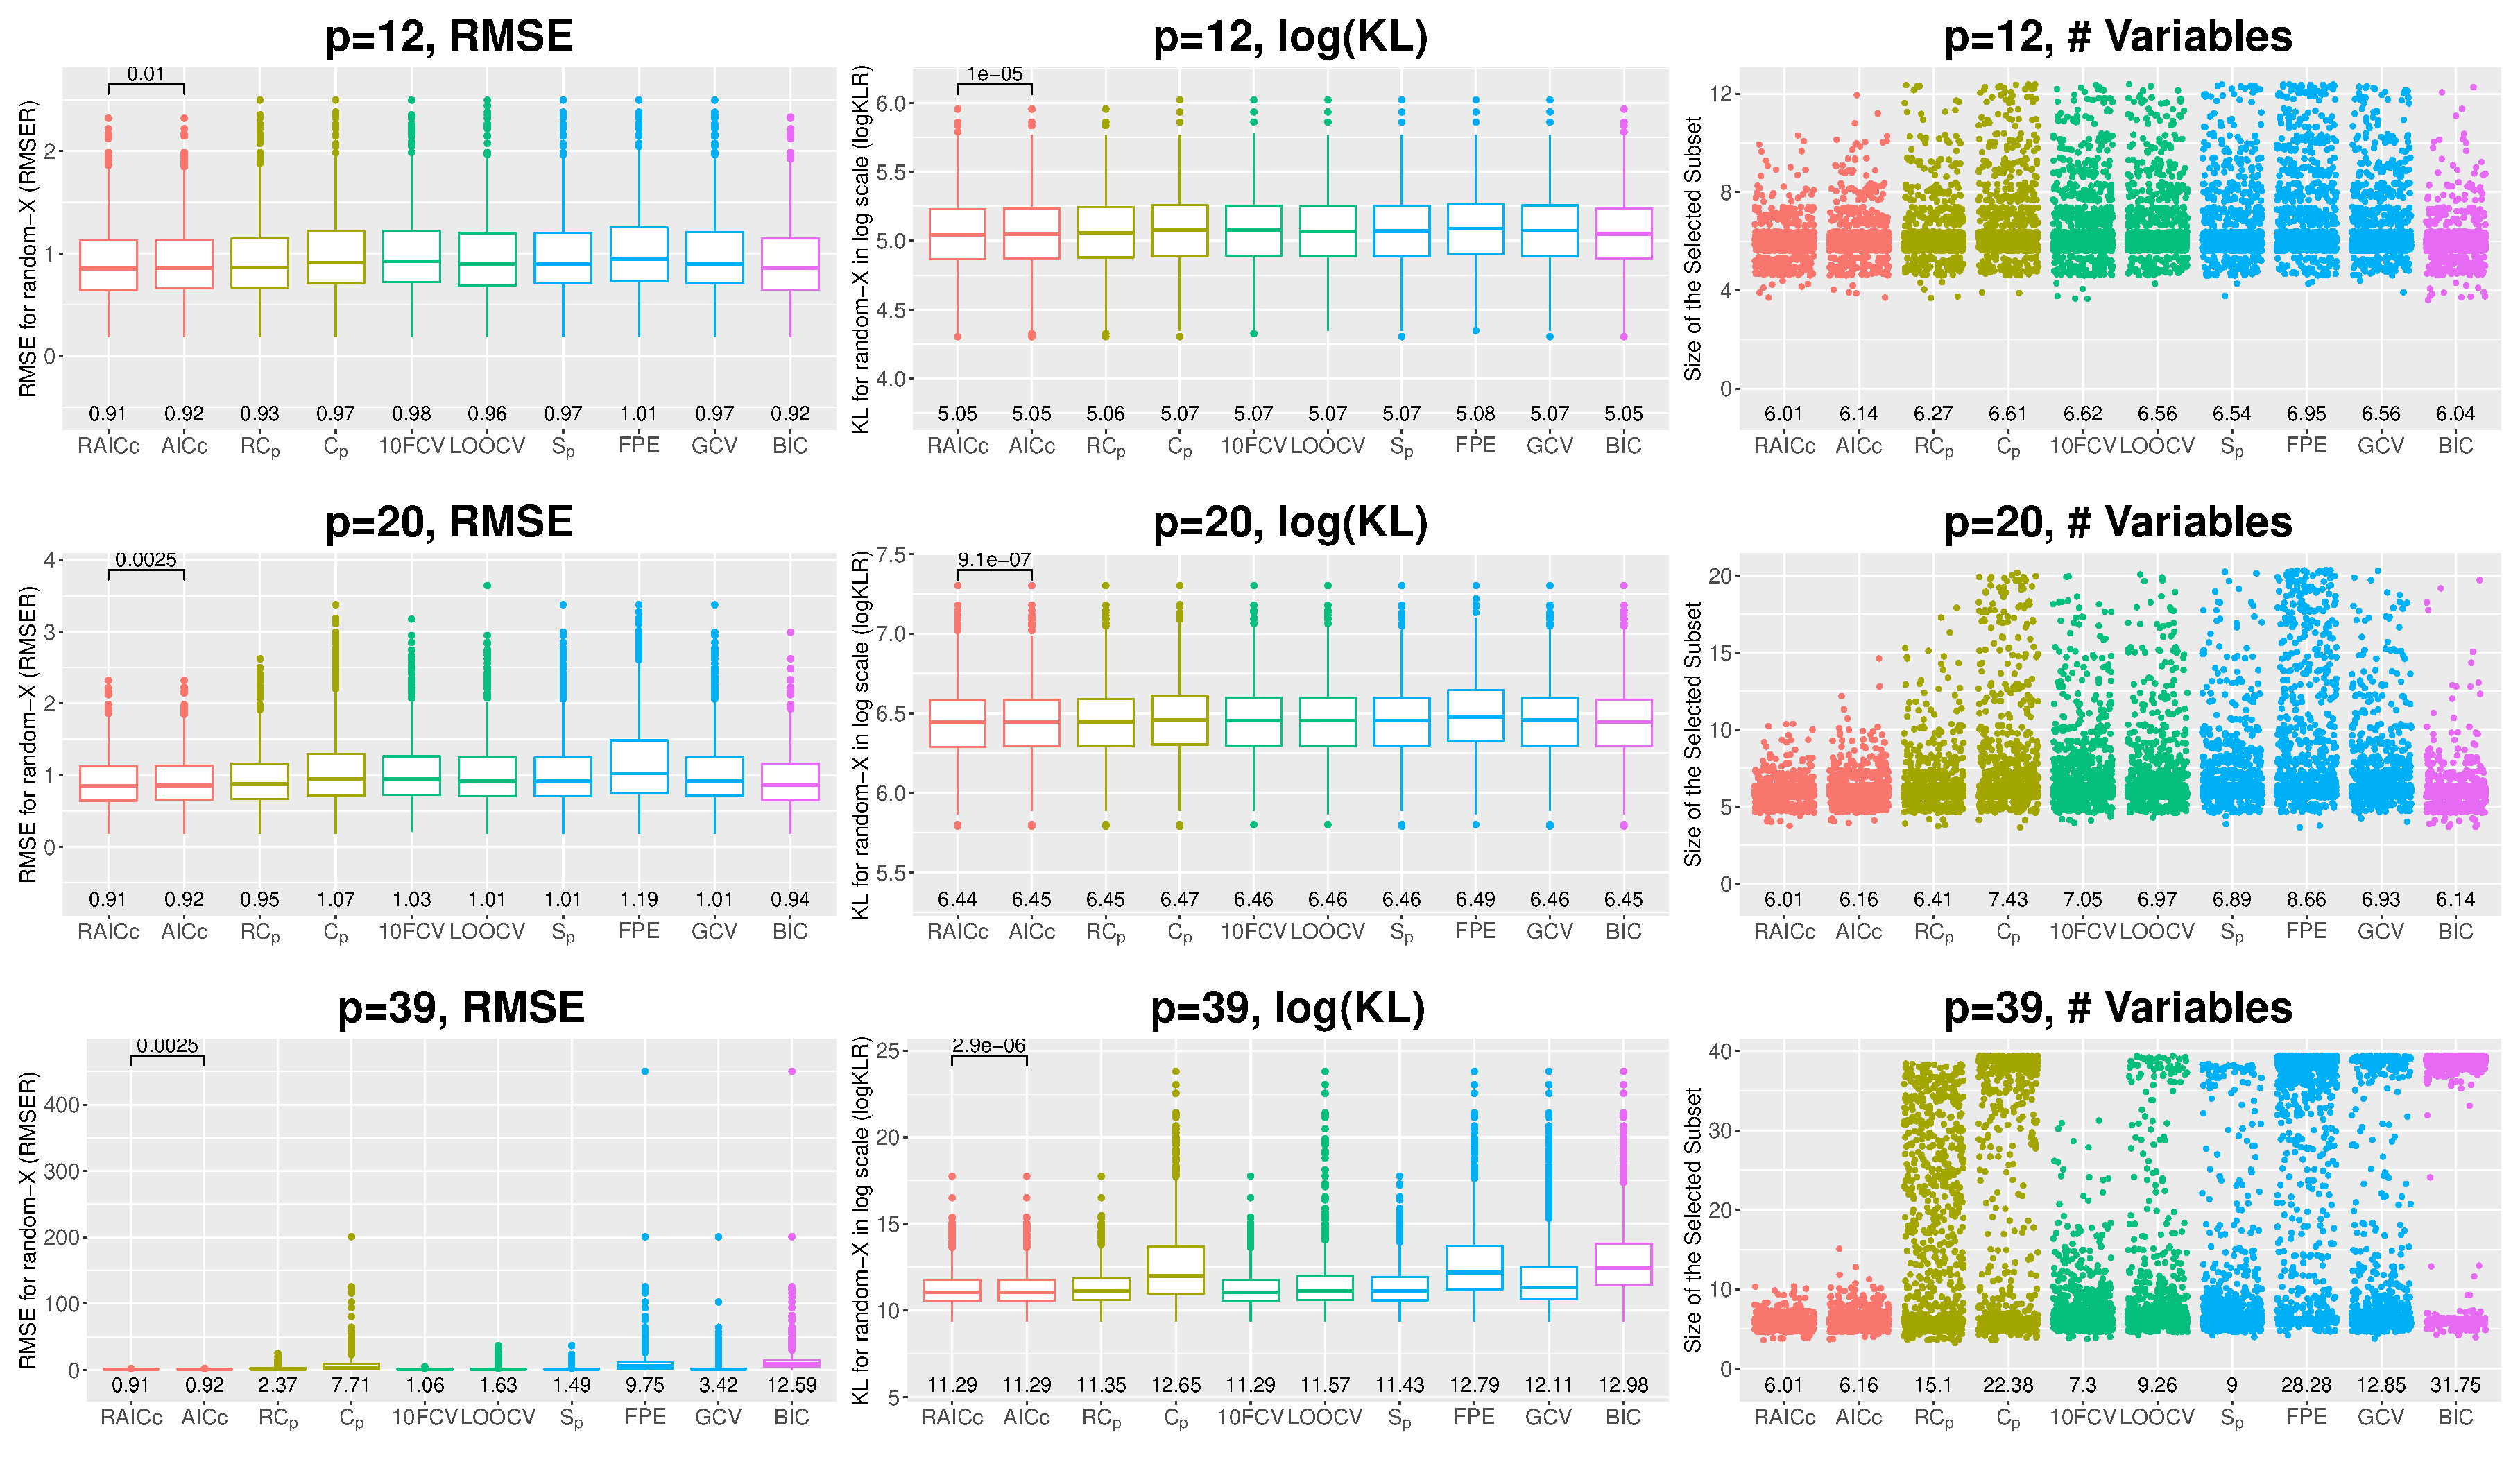
\includegraphics[width=\textwidth]{figures/supplement/randomx_VS-Ex1_n40_hsnr_rho0.eps}
\caption{VS-Ex1, $n=40$, high signal, $\rho=0$, and Random-X.}
\end{figure}
\begin{figure}[!ht]
\centering
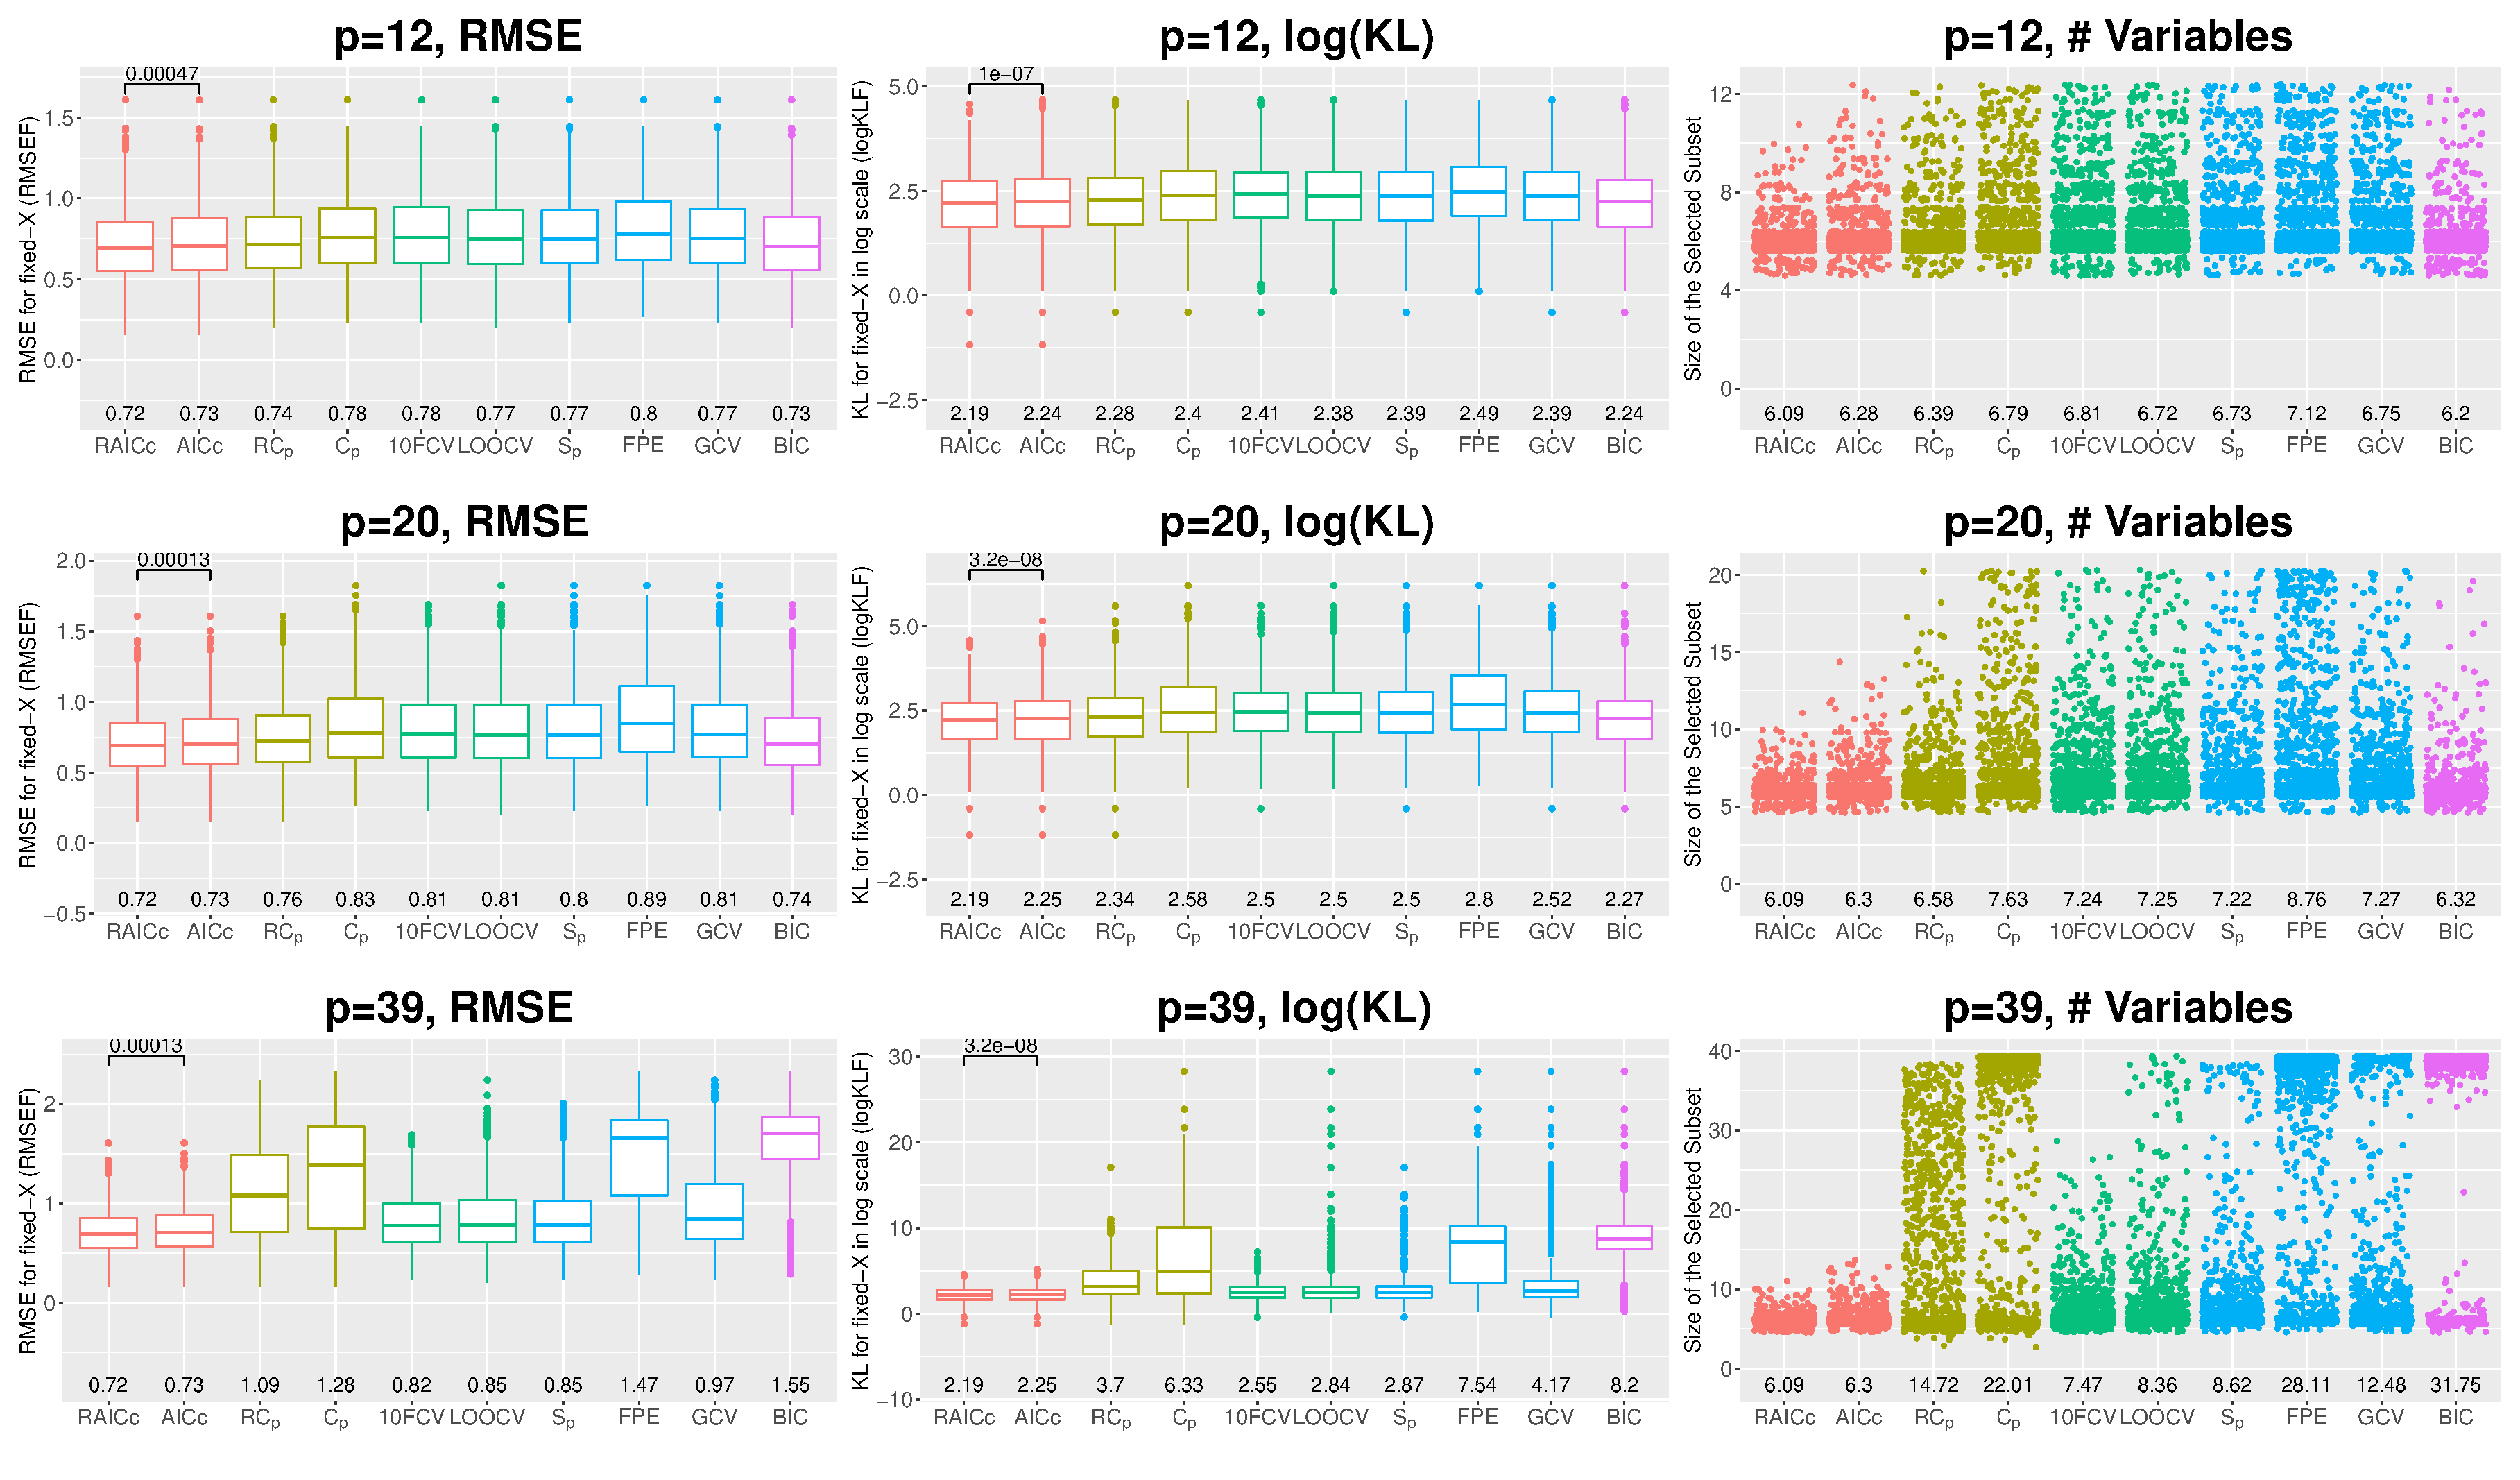
\includegraphics[width=\textwidth]{figures/supplement/fixedx_VS-Ex1_n40_hsnr_rho0.eps}
\caption{VS-Ex1, $n=40$, high signal, $\rho=0$, and Fixed-X.}
\end{figure}
\clearpage
\begin{figure}[!ht]
\centering
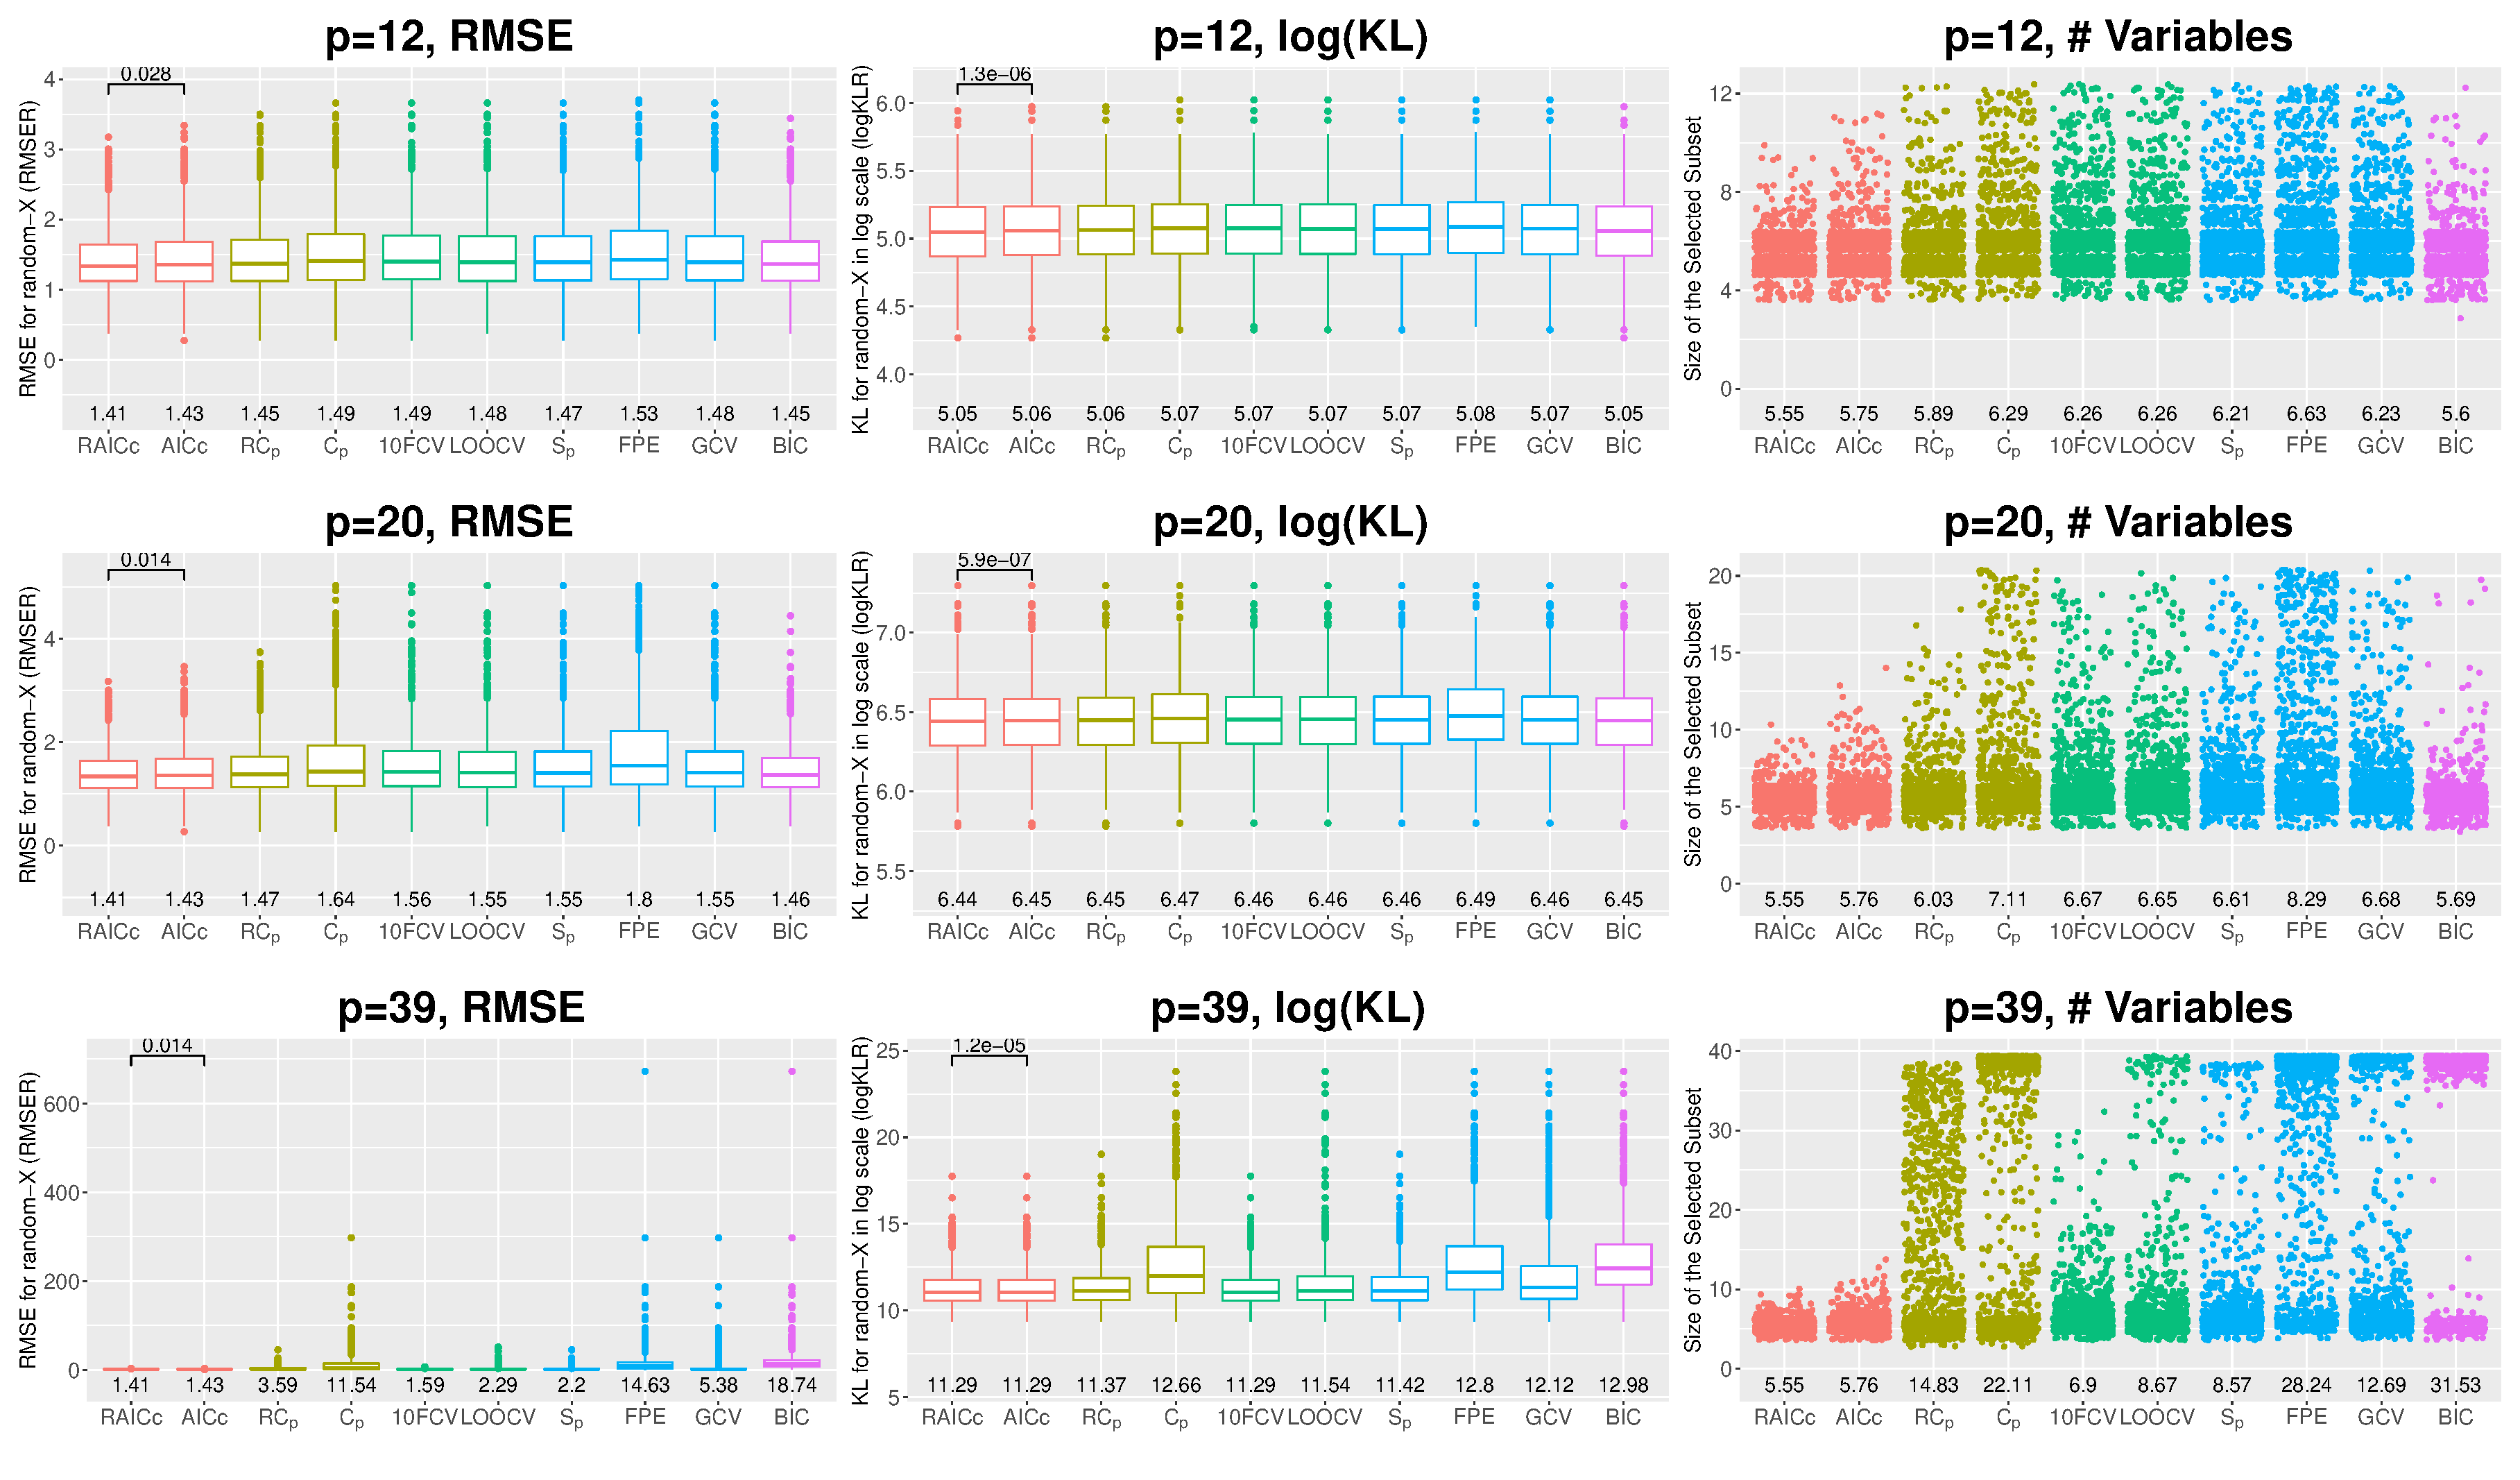
\includegraphics[width=\textwidth]{figures/supplement/randomx_VS-Ex1_n40_hsnr_rho05.eps}
\caption{VS-Ex1, $n=40$, high signal, $\rho=0.5$, and Random-X.}
\end{figure}
\begin{figure}[!ht]
\centering
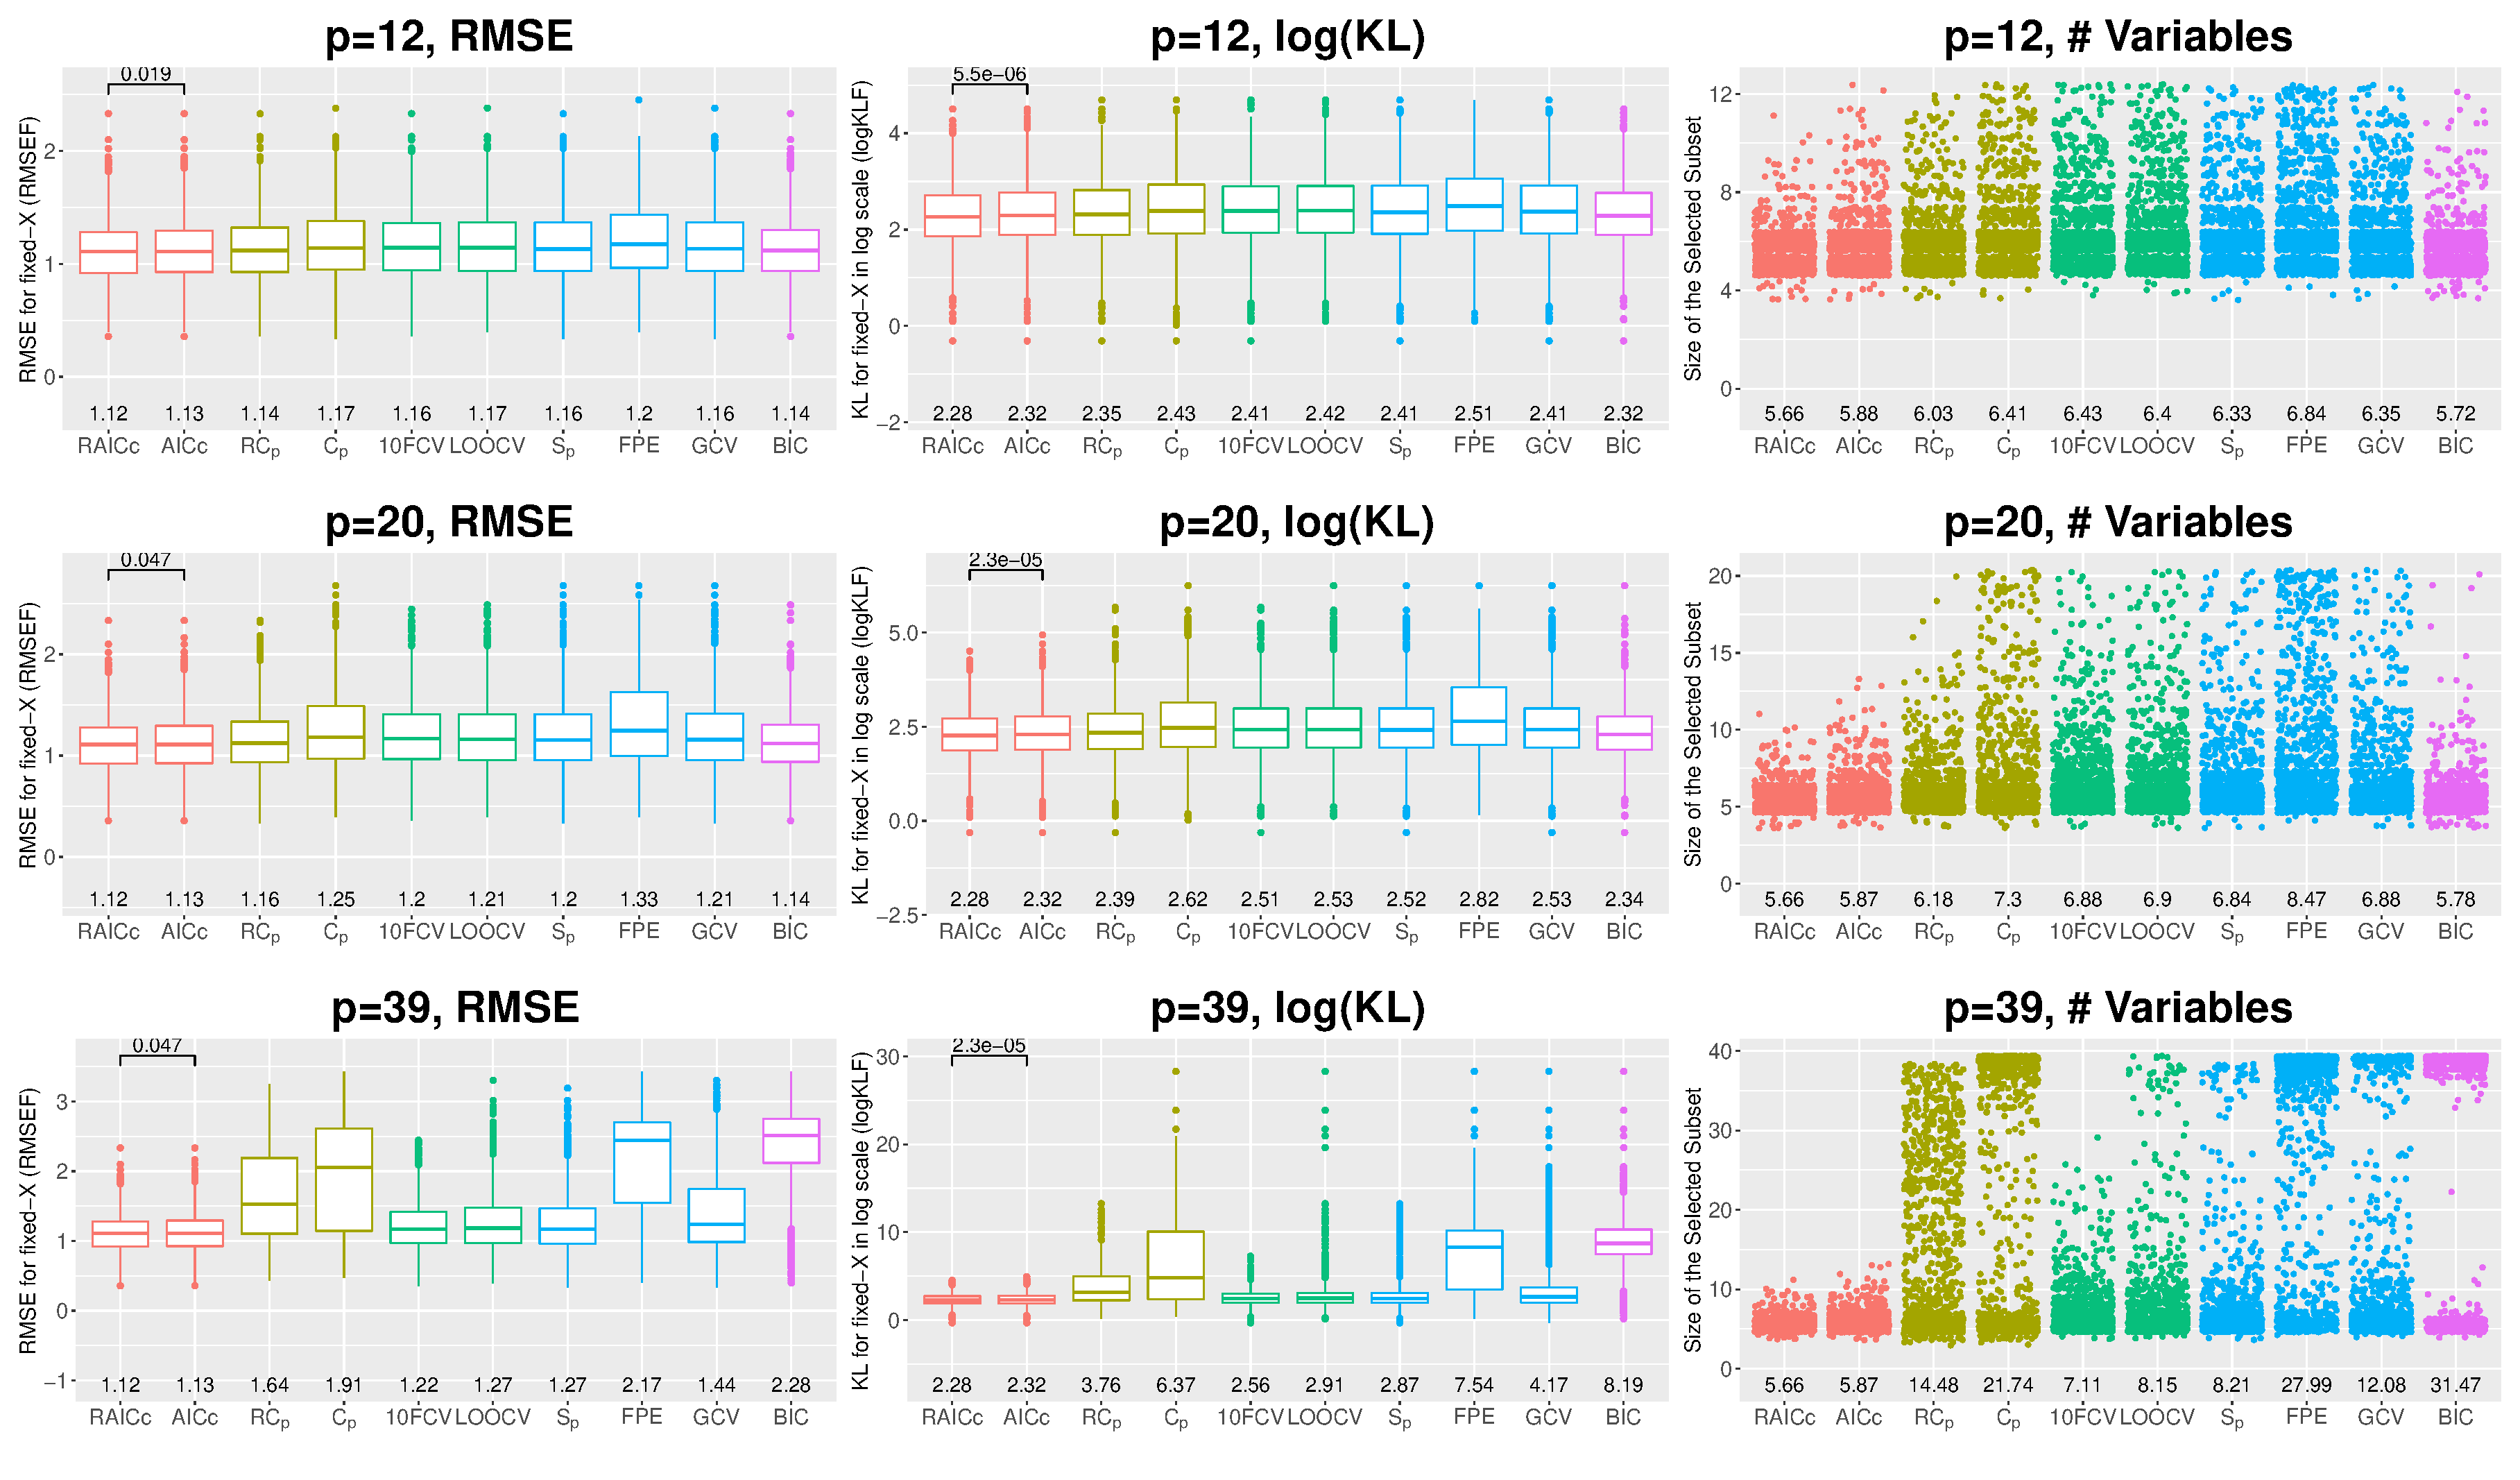
\includegraphics[width=\textwidth]{figures/supplement/fixedx_VS-Ex1_n40_hsnr_rho05.eps}
\caption{VS-Ex1, $n=40$, high signal, $\rho=0.5$, and Fixed-X.}
\end{figure}
\clearpage
\begin{figure}[!ht]
\centering
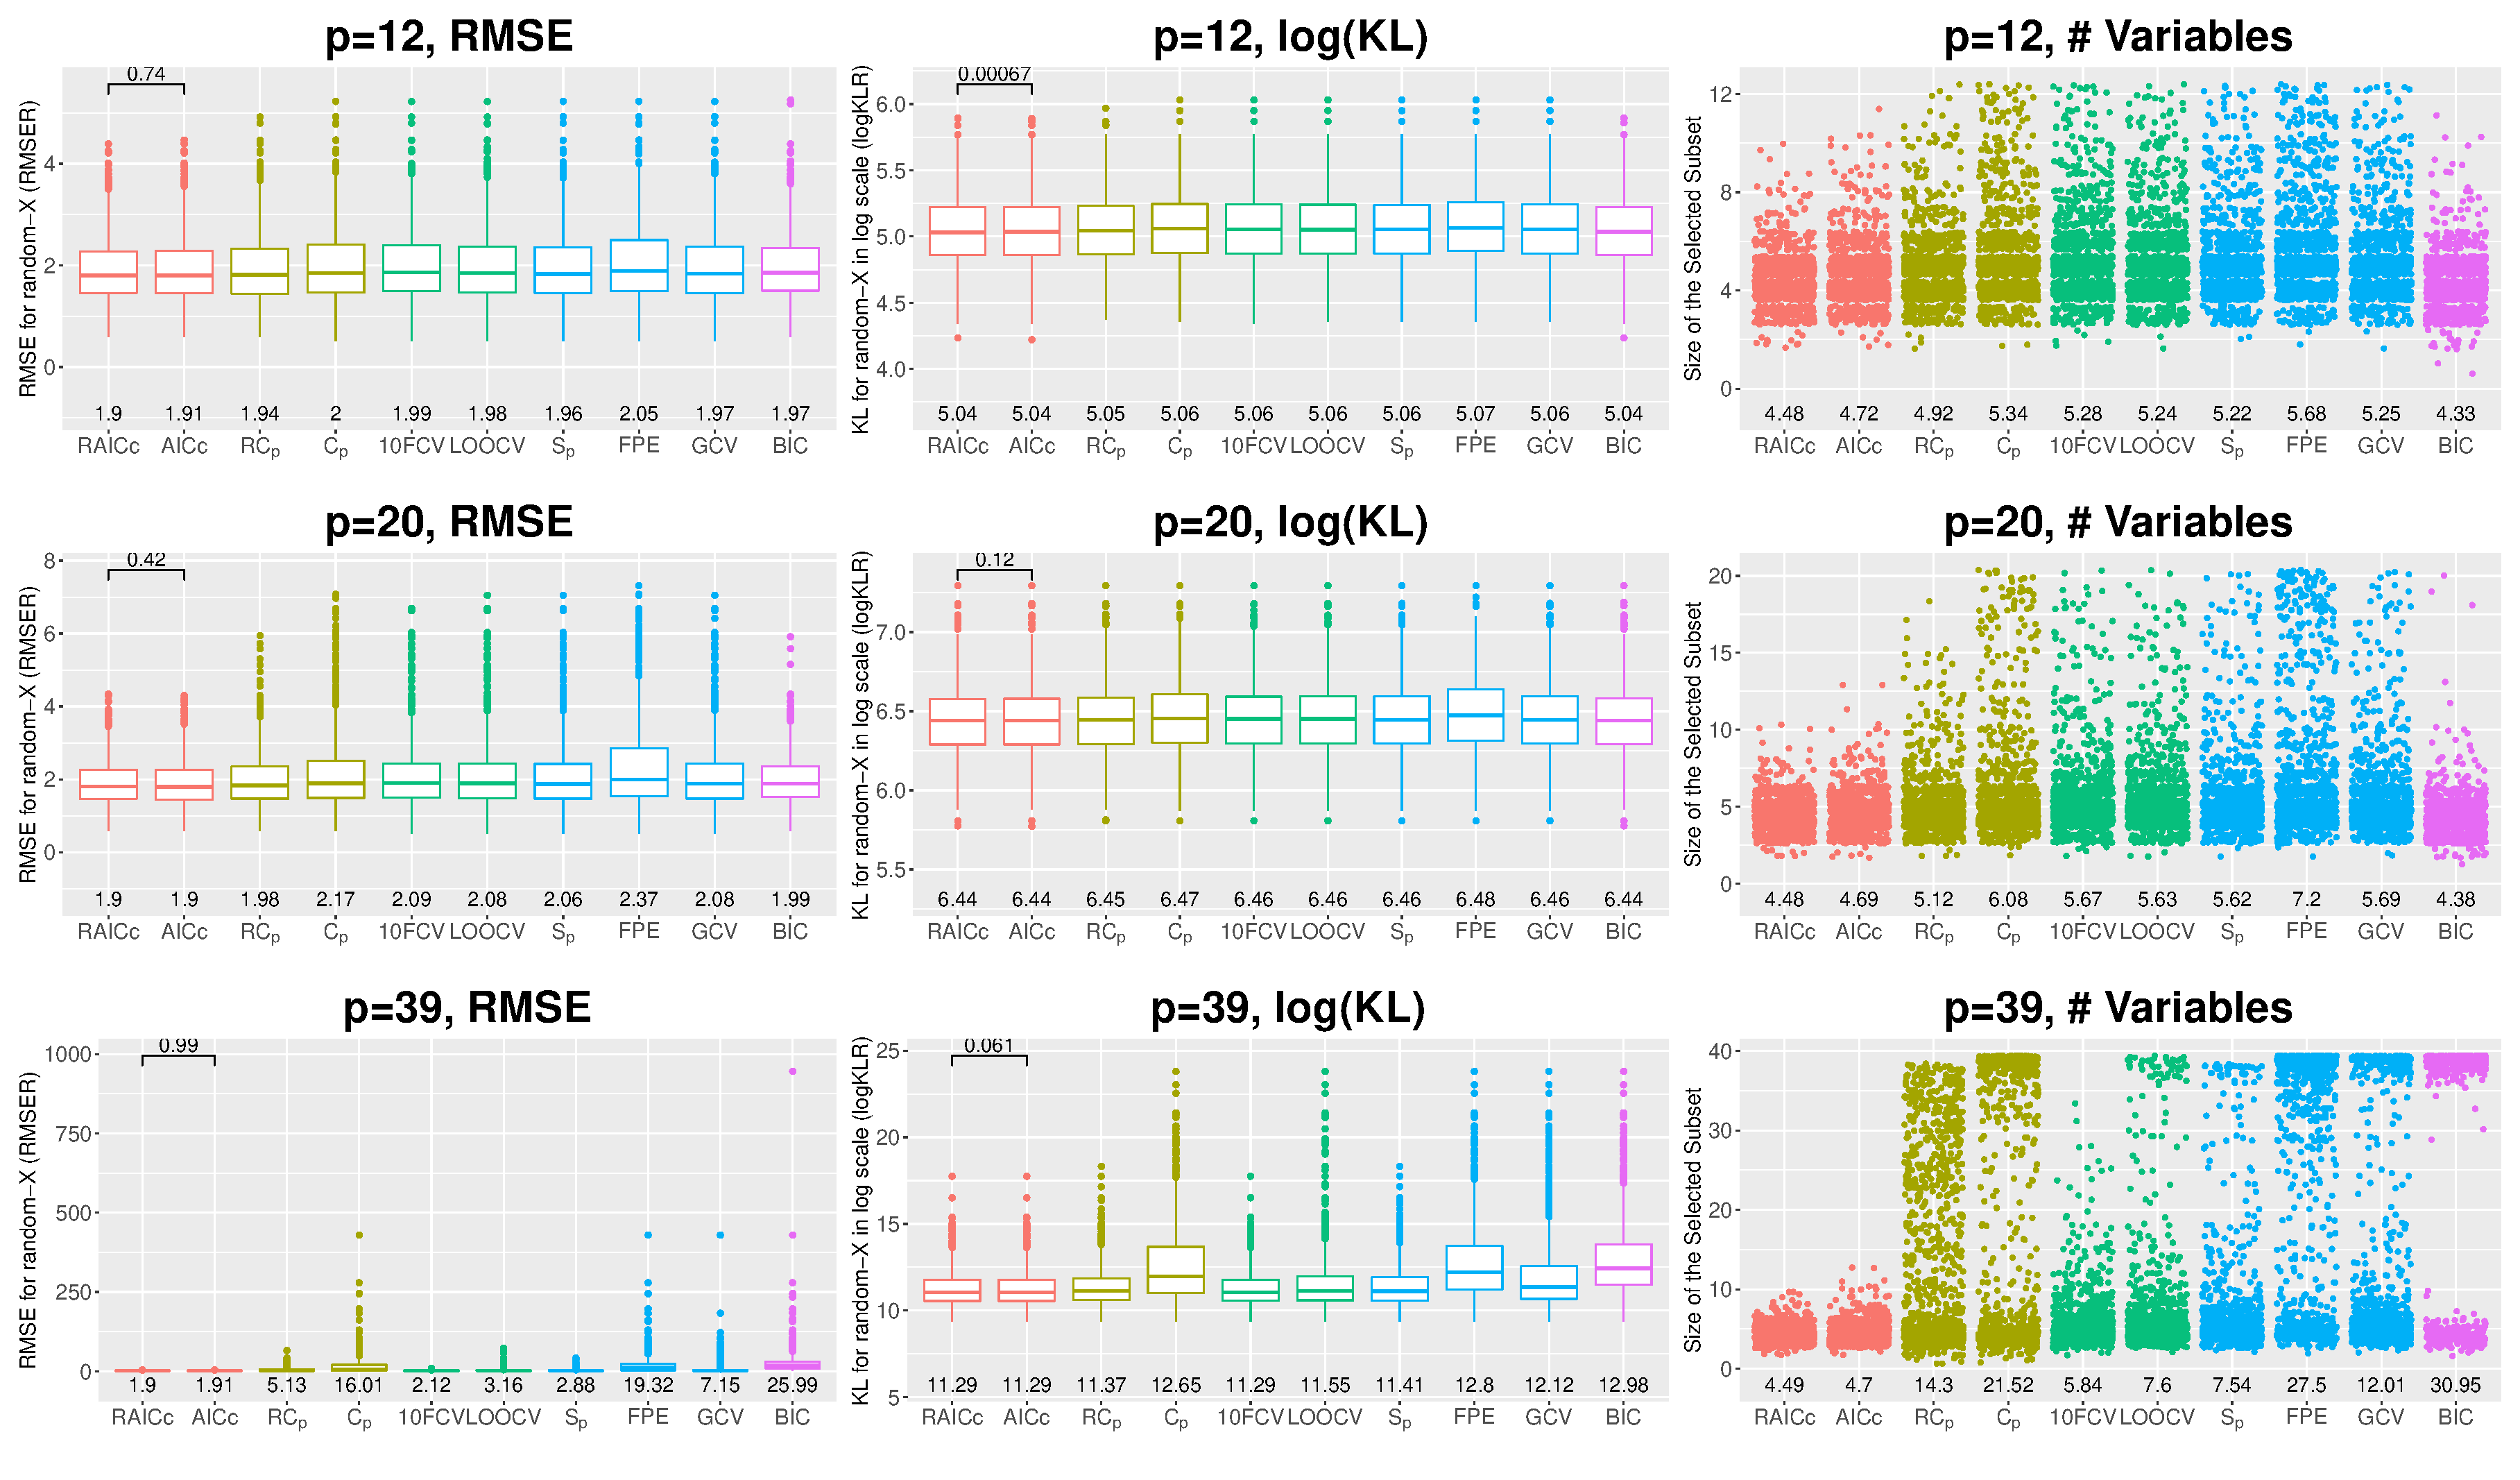
\includegraphics[width=\textwidth]{figures/supplement/randomx_VS-Ex1_n40_hsnr_rho09.eps}
\caption{VS-Ex1, $n=40$, high signal, $\rho=0.9$, and Random-X.}
\end{figure}
\begin{figure}[!ht]
\centering
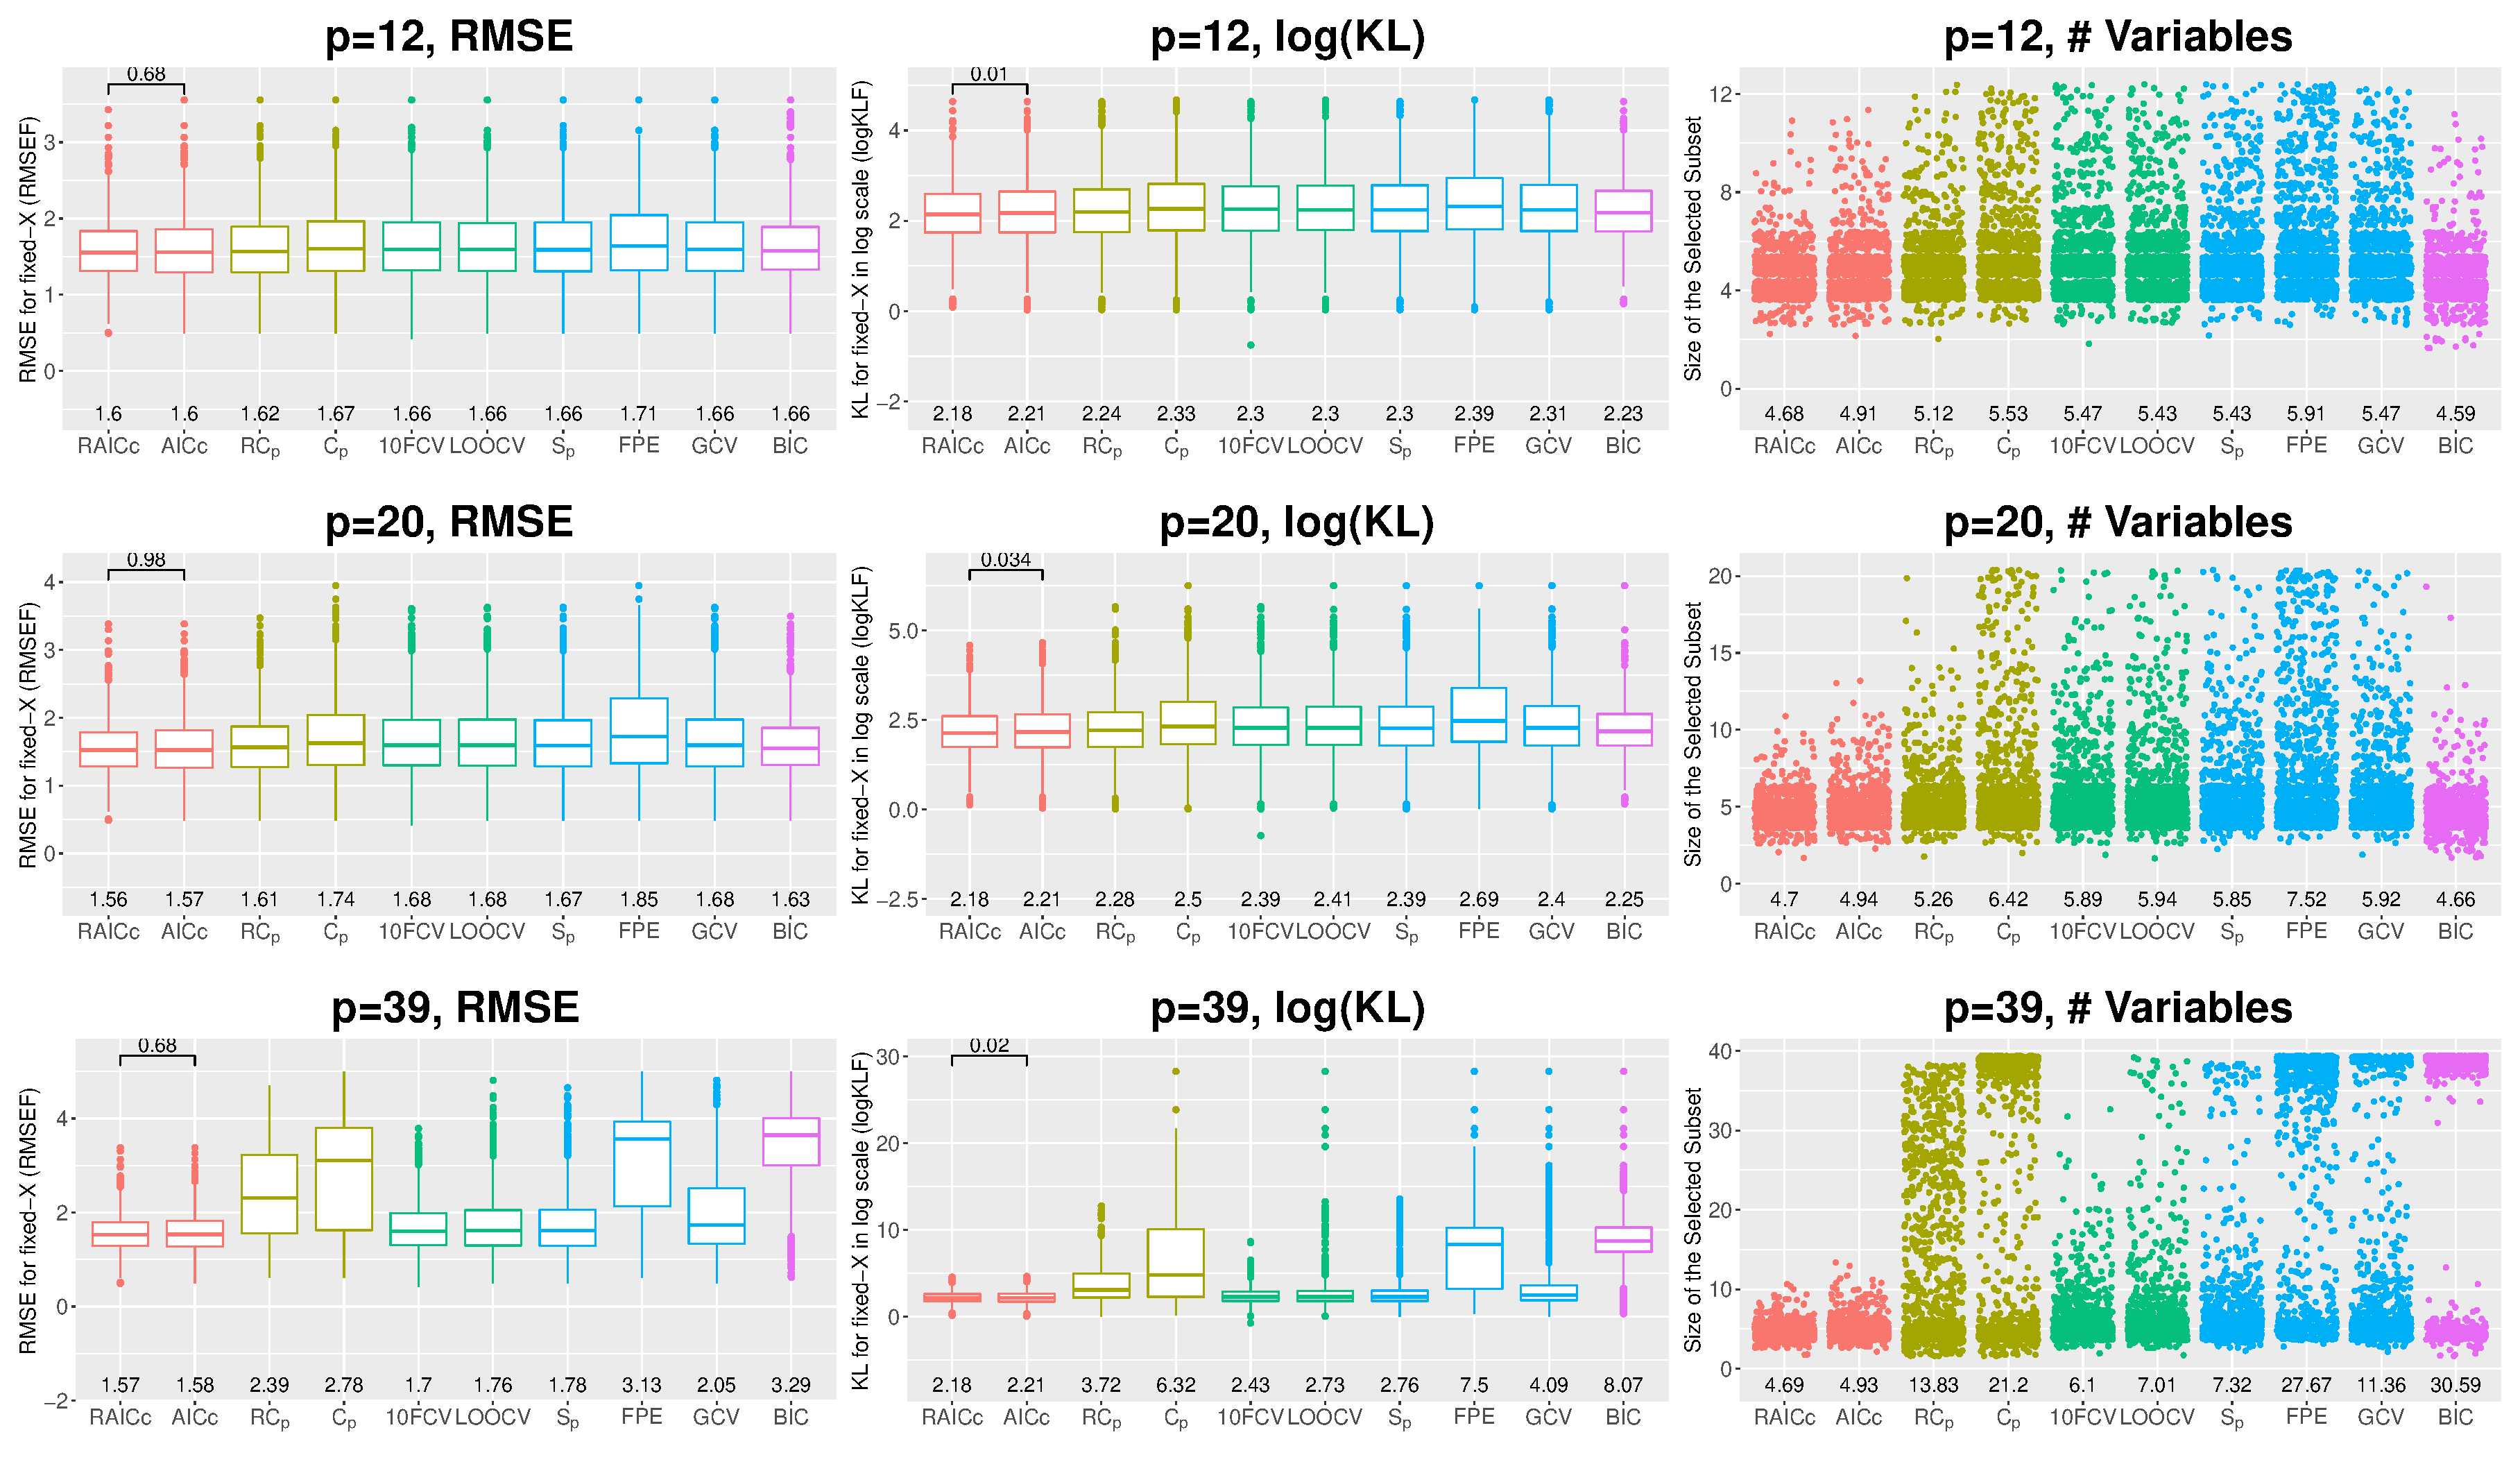
\includegraphics[width=\textwidth]{figures/supplement/fixedx_VS-Ex1_n40_hsnr_rho09.eps}
\caption{VS-Ex1, $n=40$, high signal, $\rho=0.9$, and Fixed-X.}
\end{figure}
\clearpage
\begin{figure}[!ht]
\centering
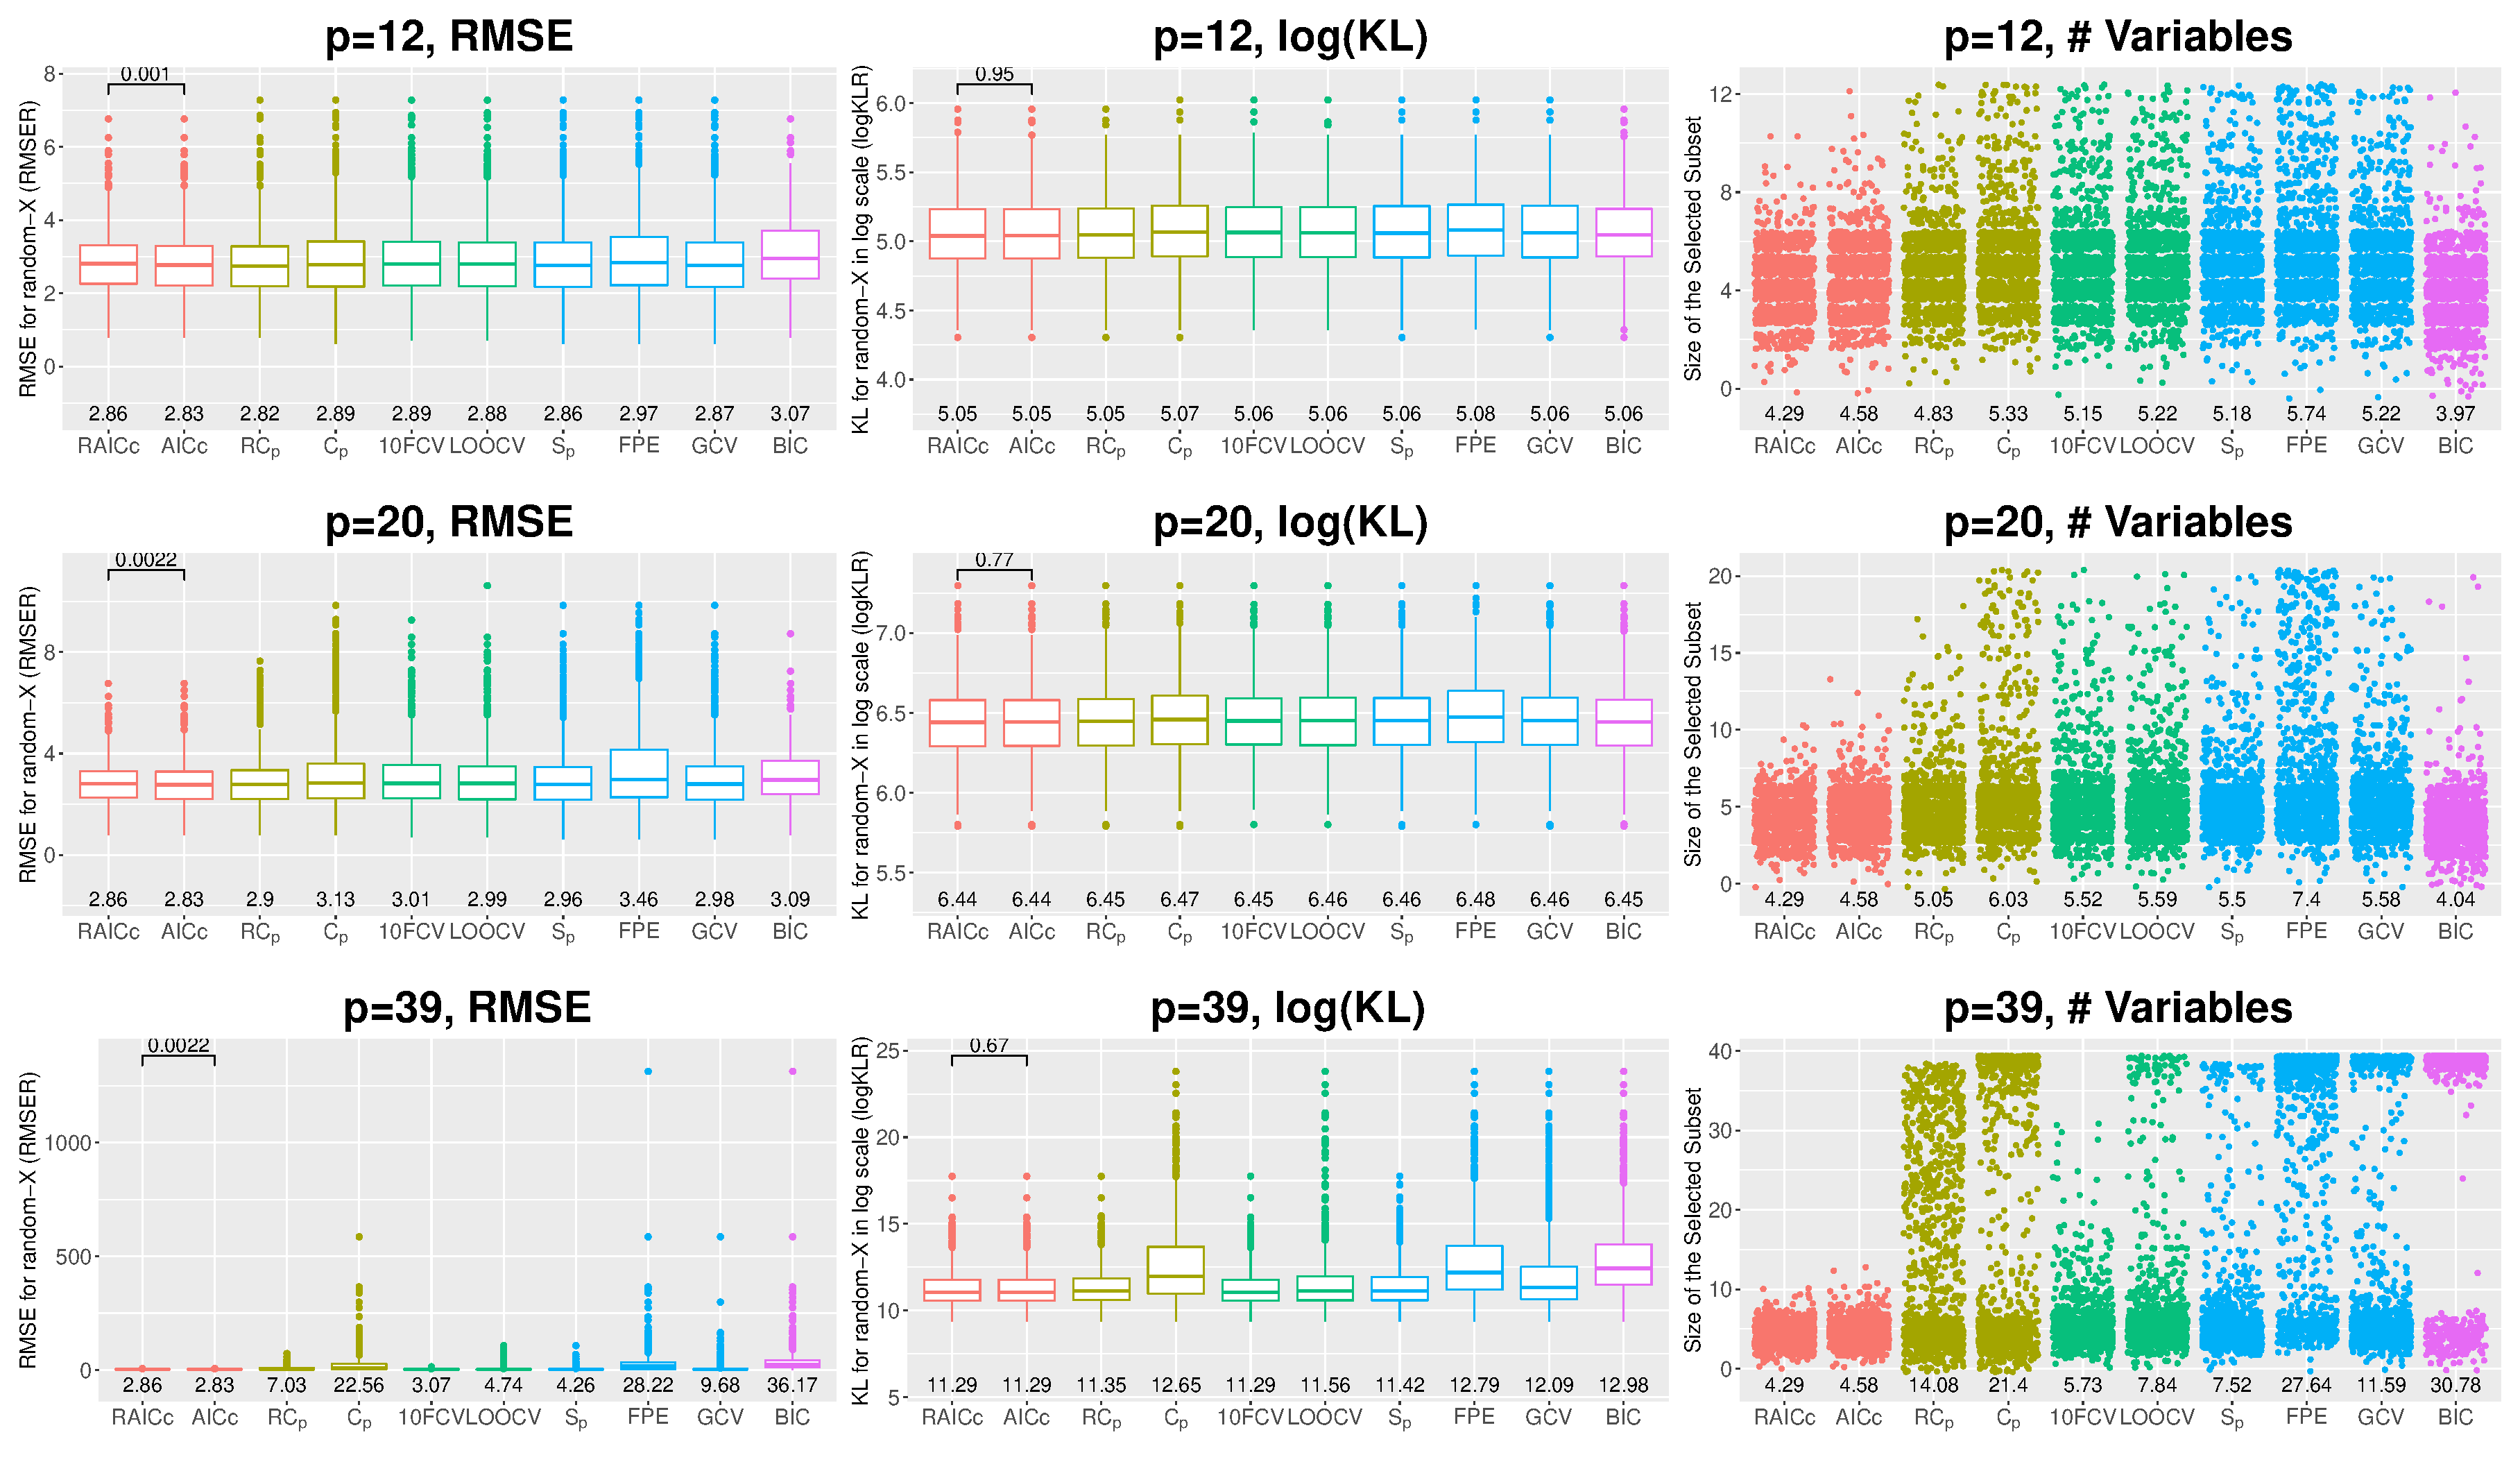
\includegraphics[width=\textwidth]{figures/supplement/randomx_VS-Ex1_n40_msnr_rho0.eps}
\caption{VS-Ex1, $n=40$, medium signal, $\rho=0$, and Random-X.}
\end{figure}
\begin{figure}[!ht]
\centering
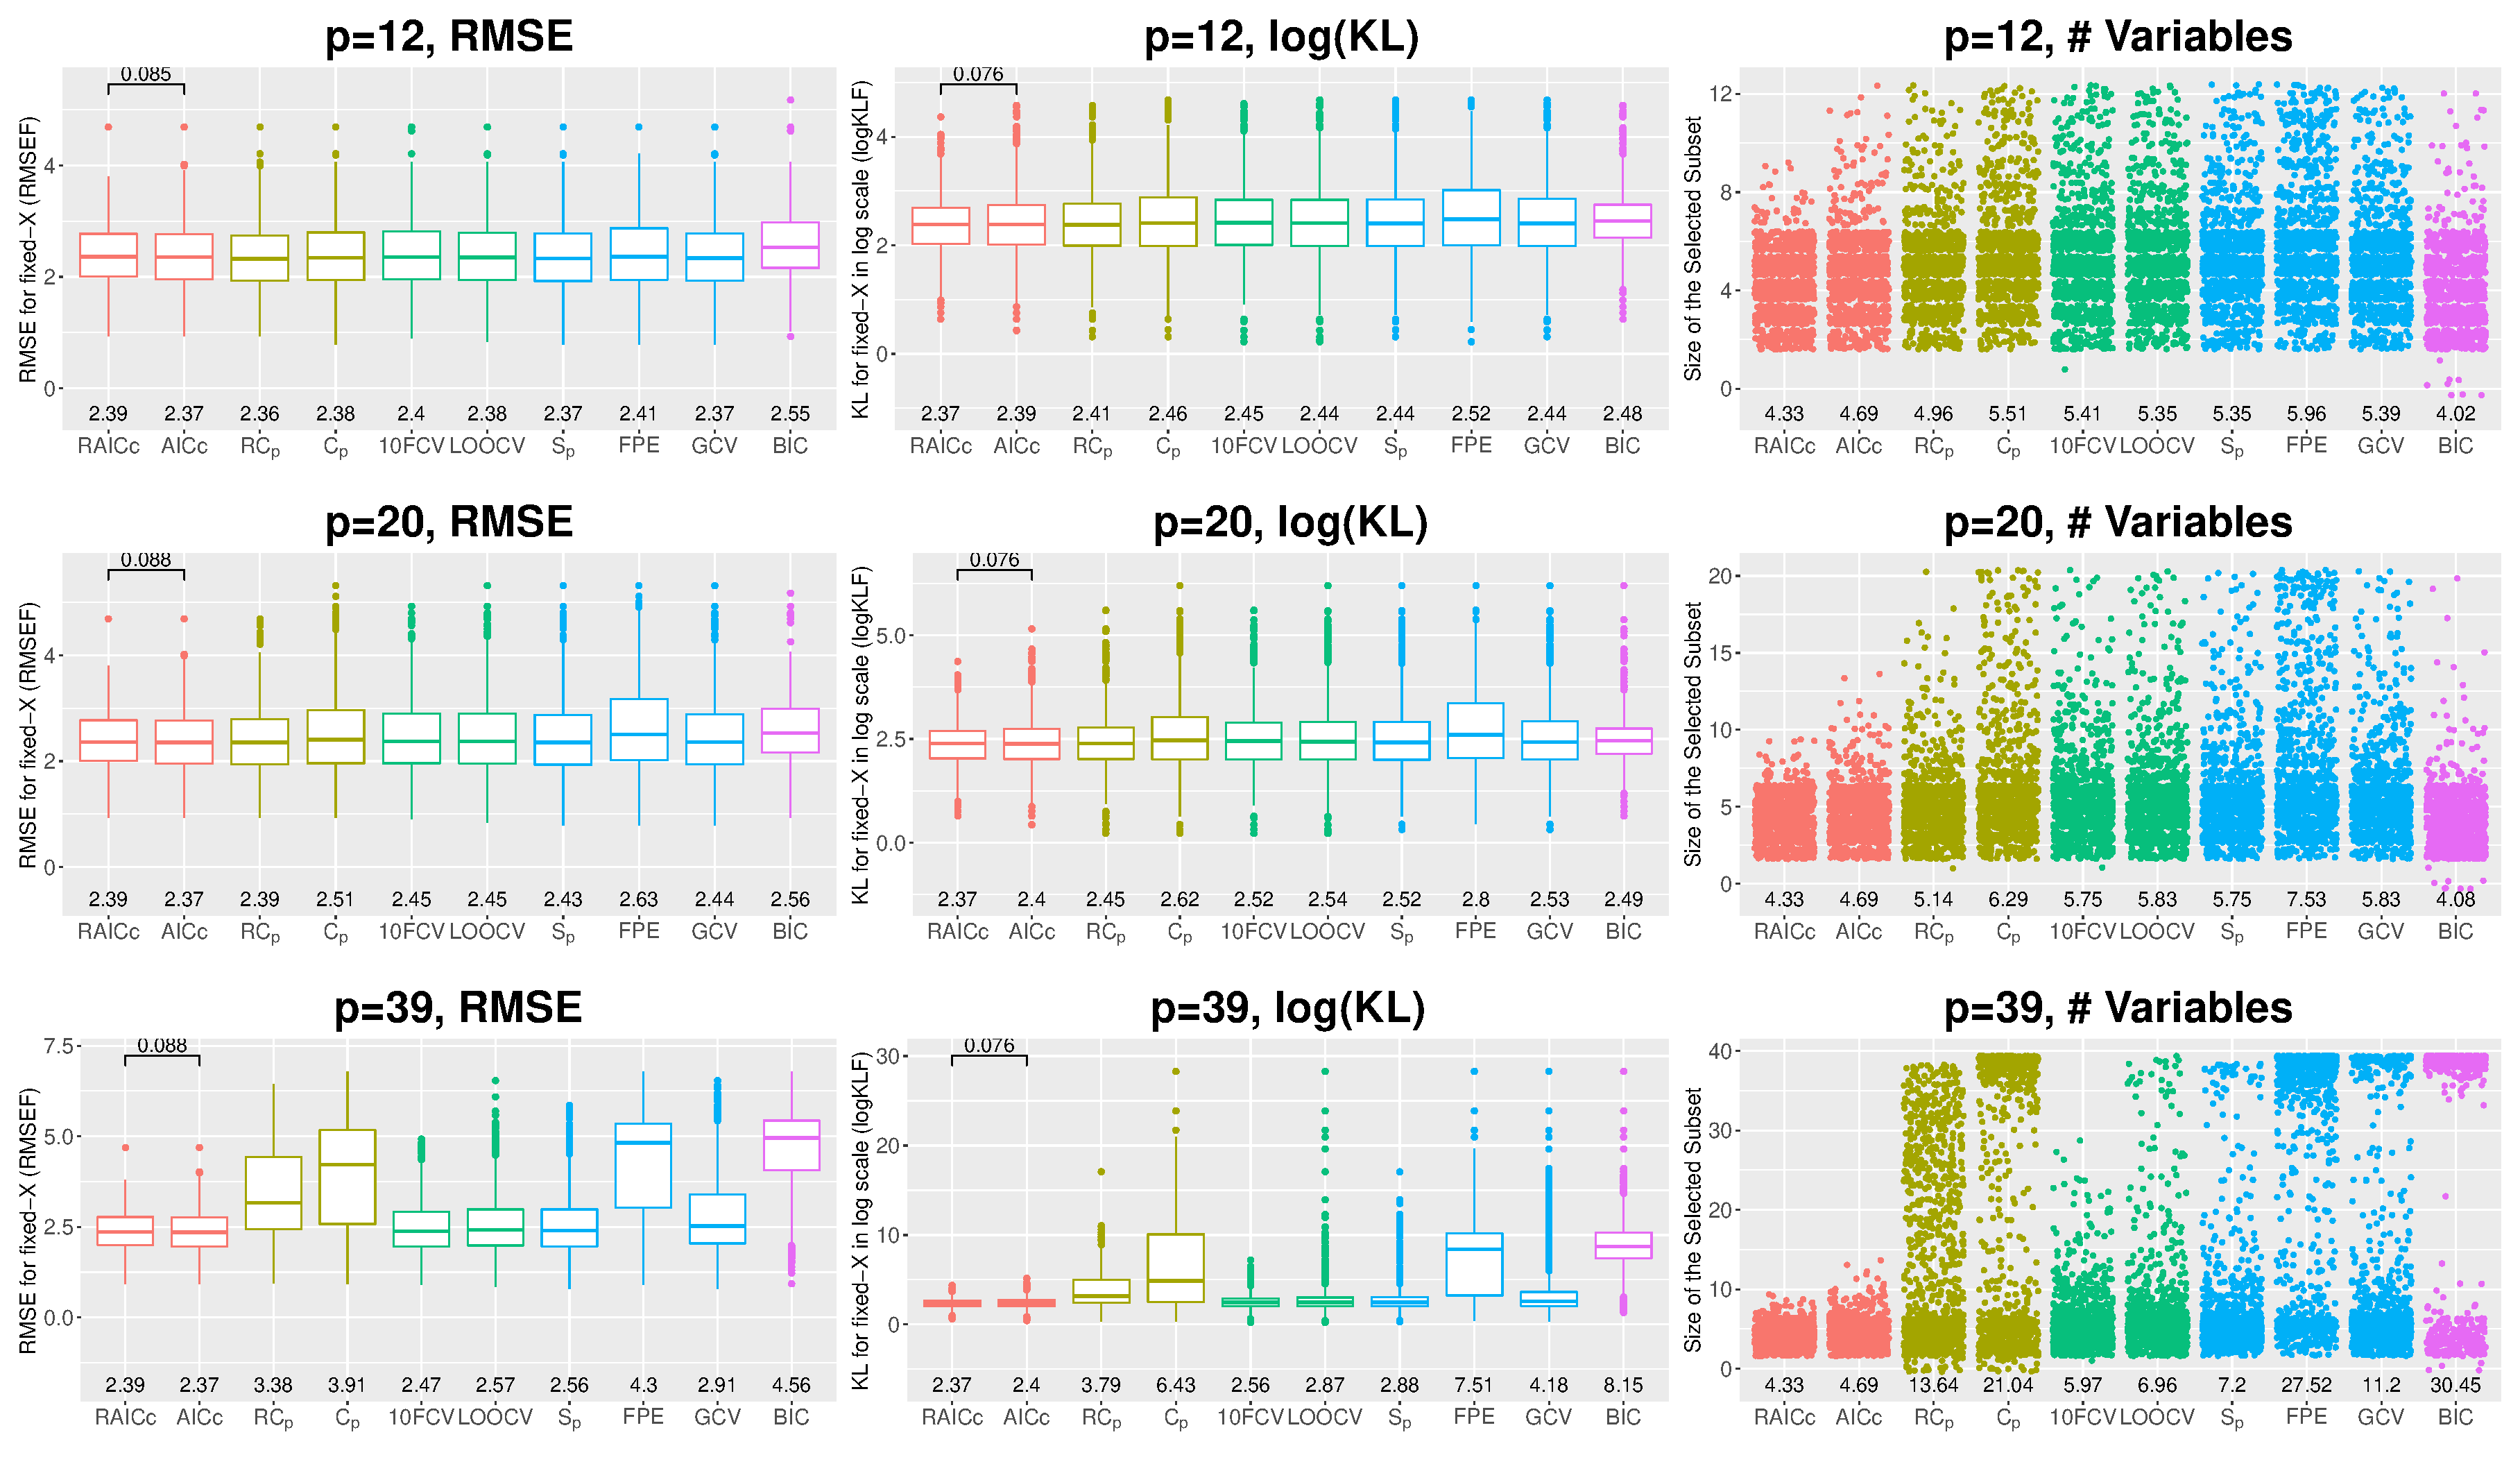
\includegraphics[width=\textwidth]{figures/supplement/fixedx_VS-Ex1_n40_msnr_rho0.eps}
\caption{VS-Ex1, $n=40$, medium signal, $\rho=0$, and Fixed-X.}
\end{figure}
\clearpage
\begin{figure}[!ht]
\centering
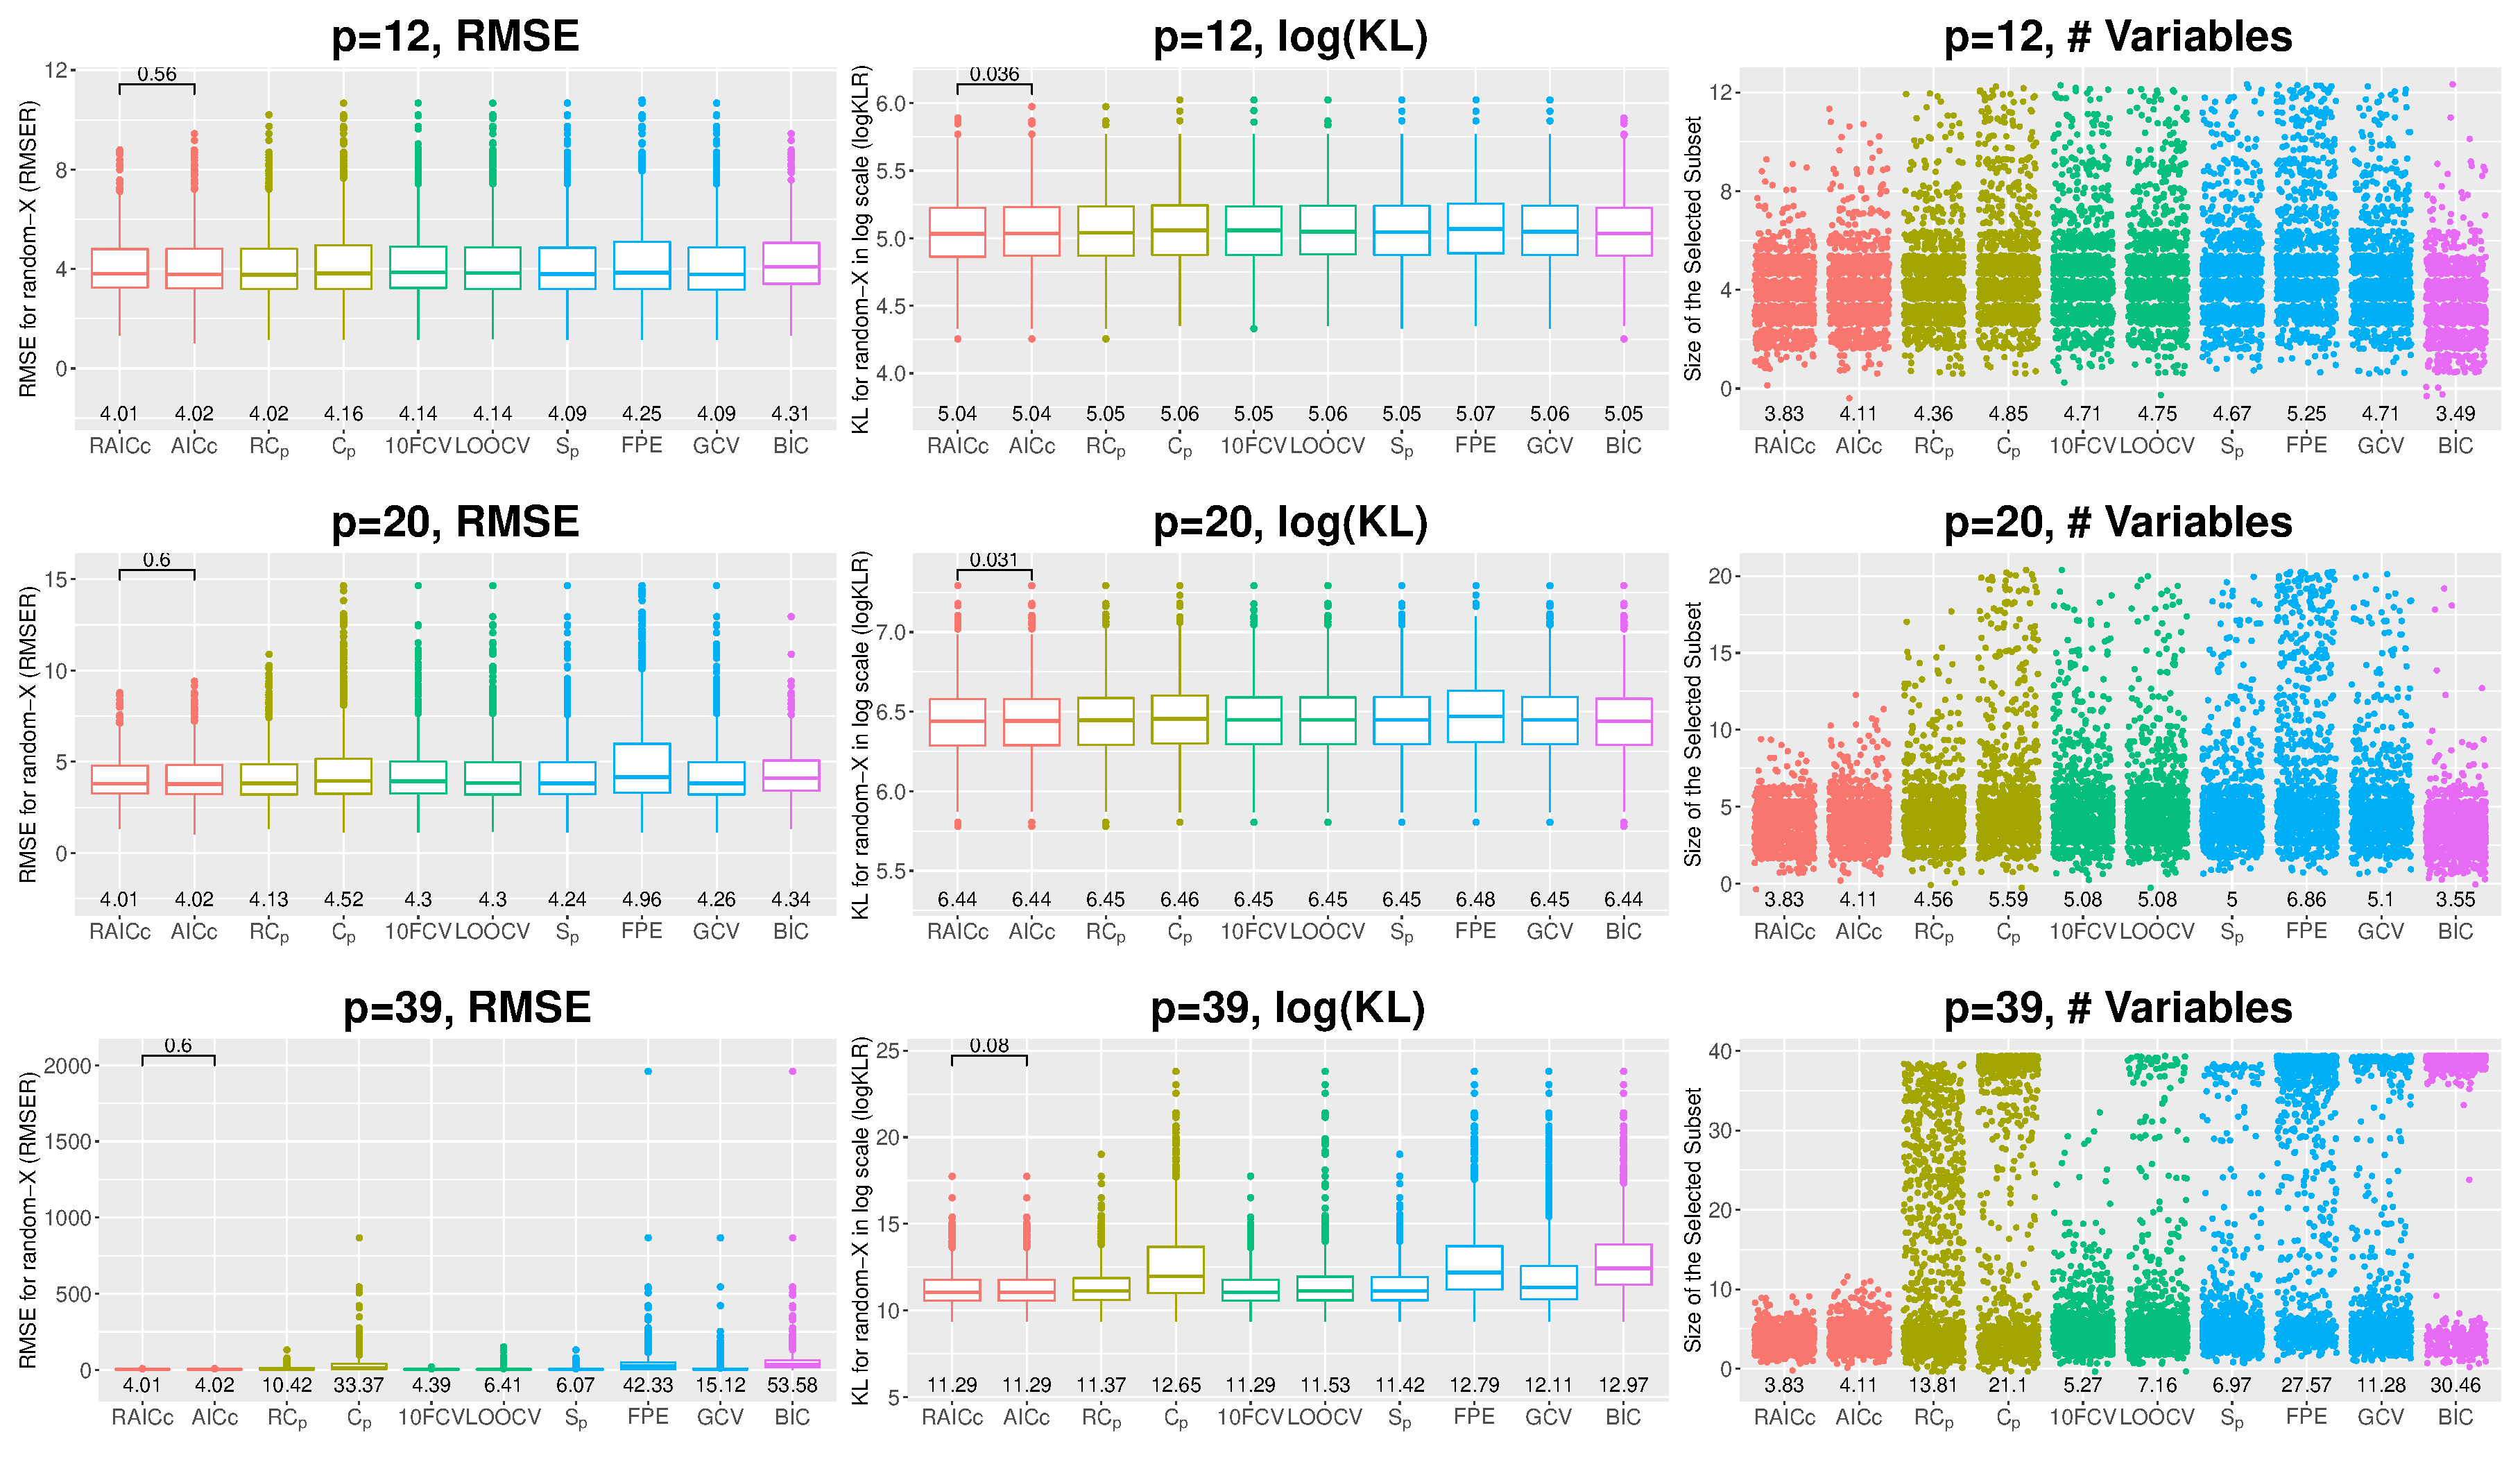
\includegraphics[width=\textwidth]{figures/supplement/randomx_VS-Ex1_n40_msnr_rho05.eps}
\caption{VS-Ex1, $n=40$, medium signal, $\rho=0.5$, and Random-X.}
\end{figure}
\begin{figure}[!ht]
\centering
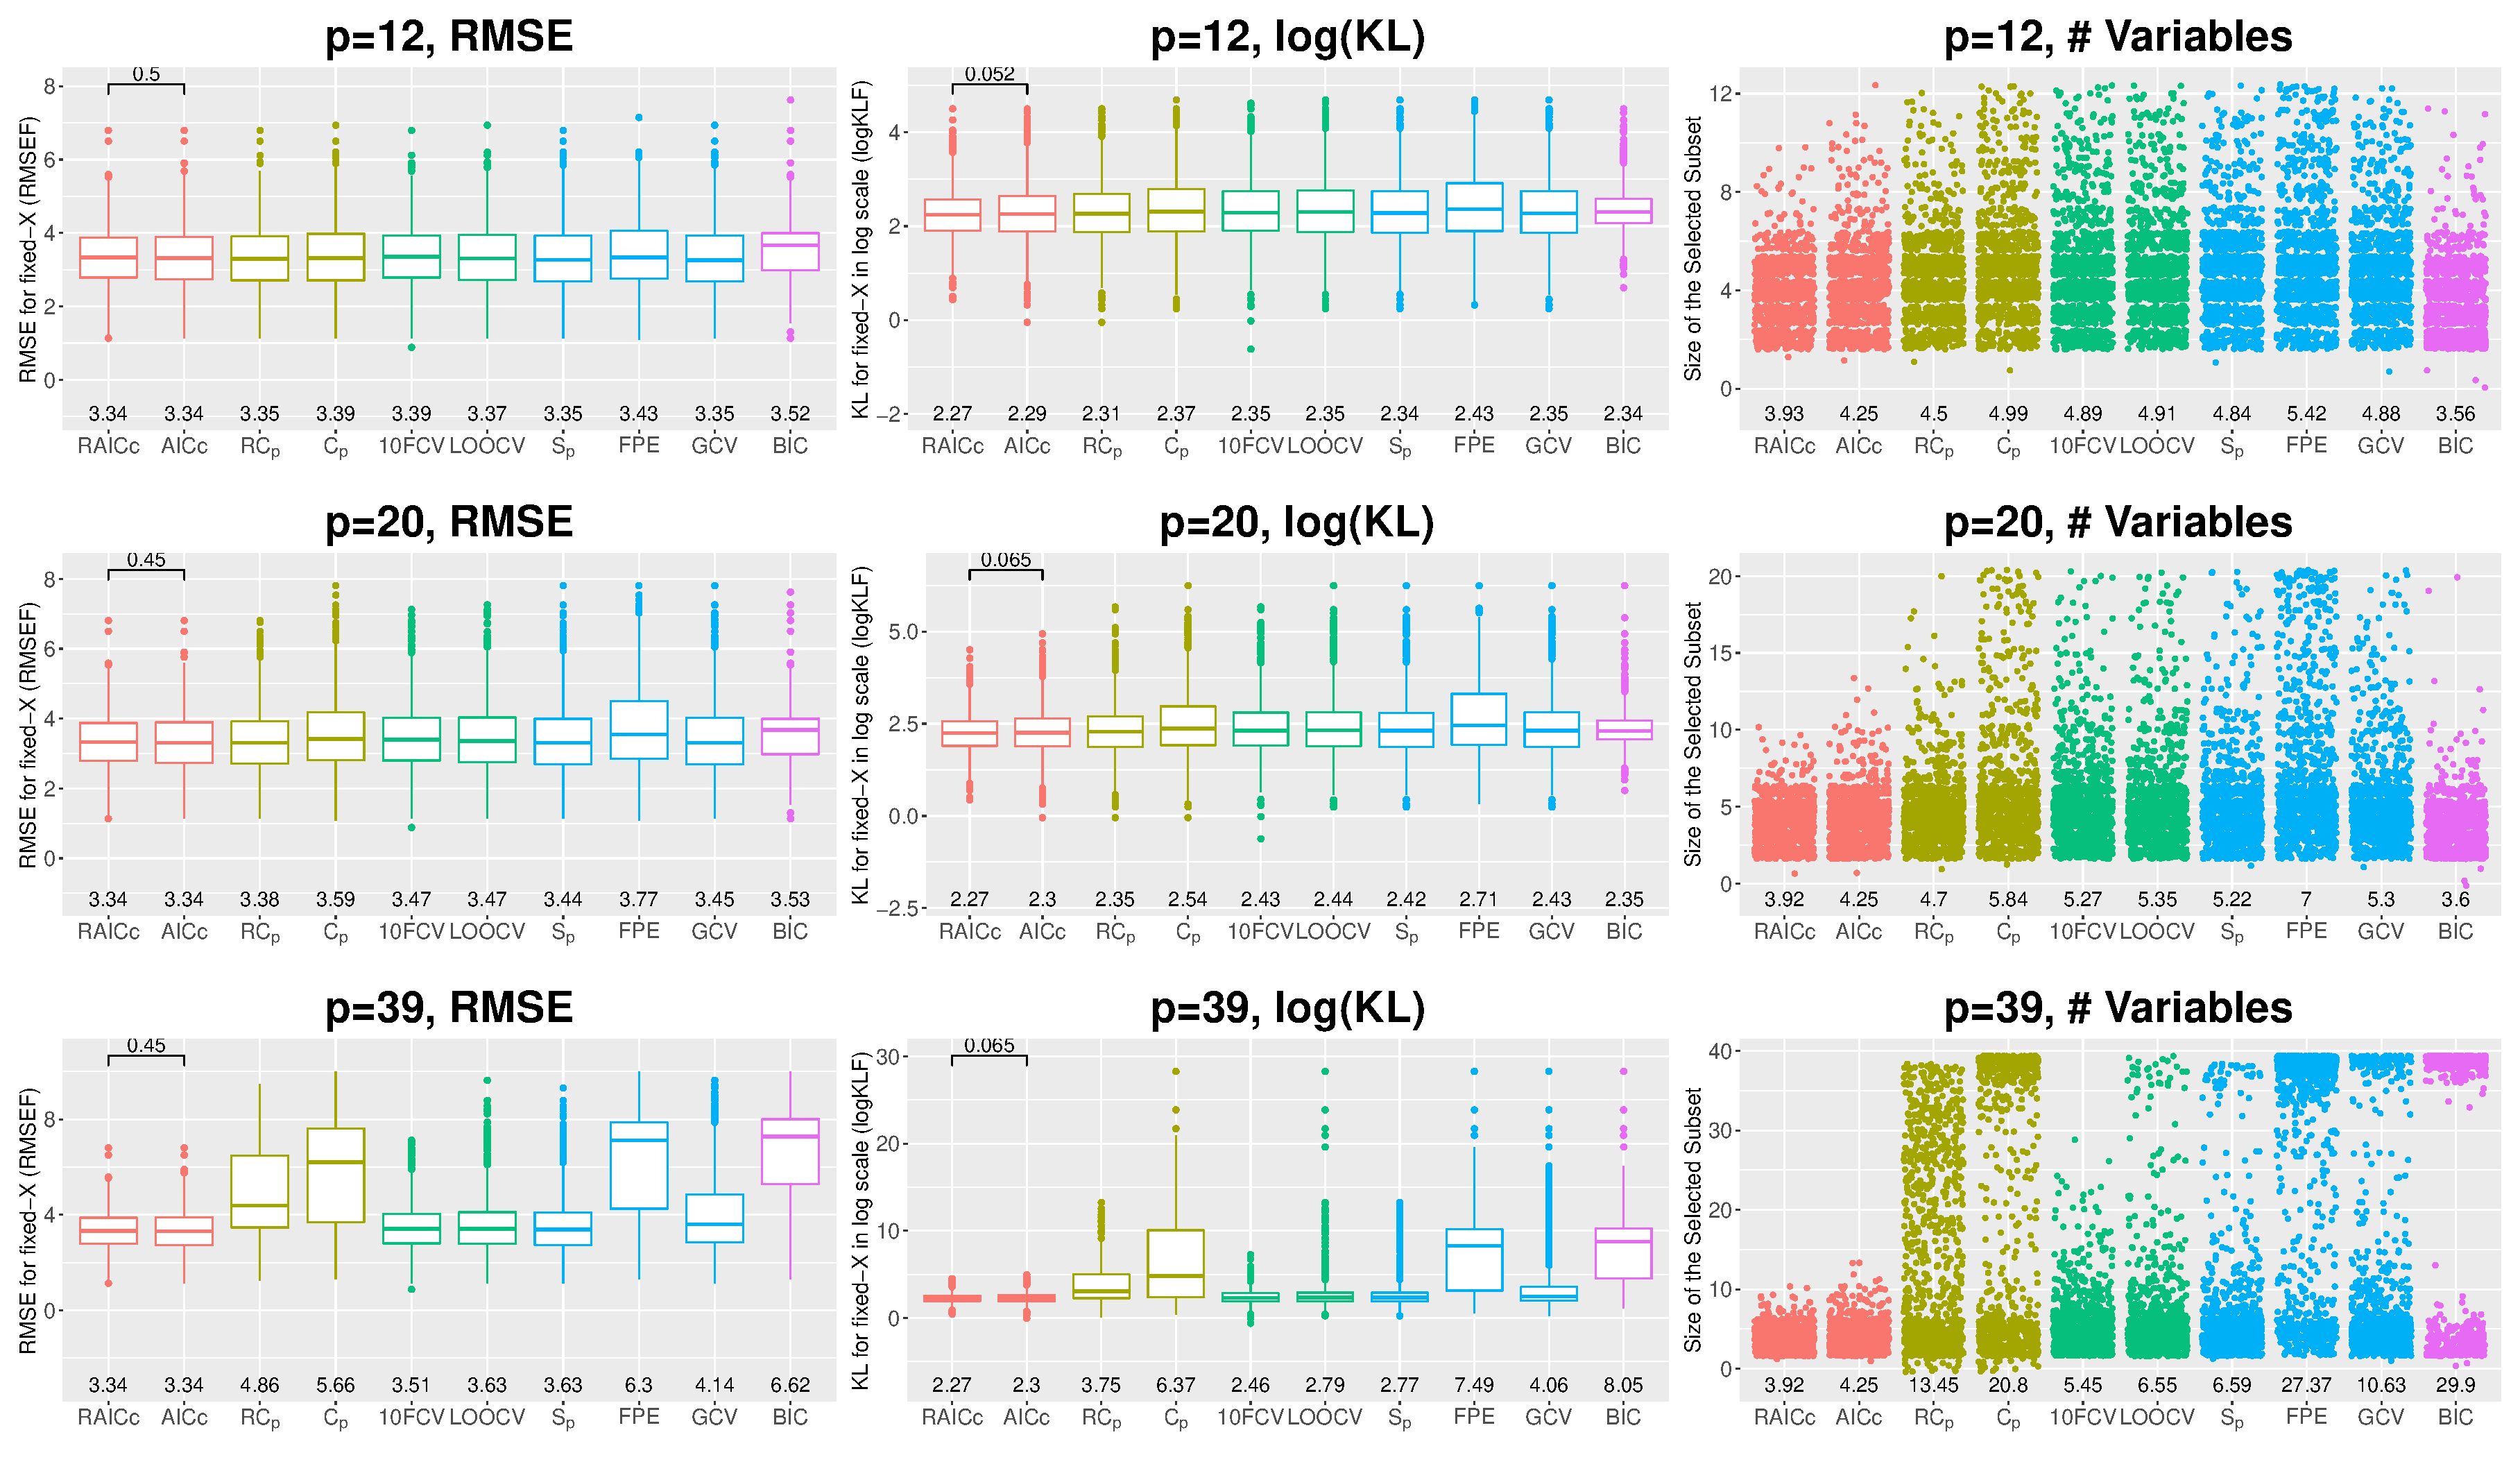
\includegraphics[width=\textwidth]{figures/supplement/fixedx_VS-Ex1_n40_msnr_rho05.eps}
\caption{VS-Ex1, $n=40$, medium signal, $\rho=0.5$, and Fixed-X.}
\end{figure}
\clearpage
\begin{figure}[!ht]
\centering
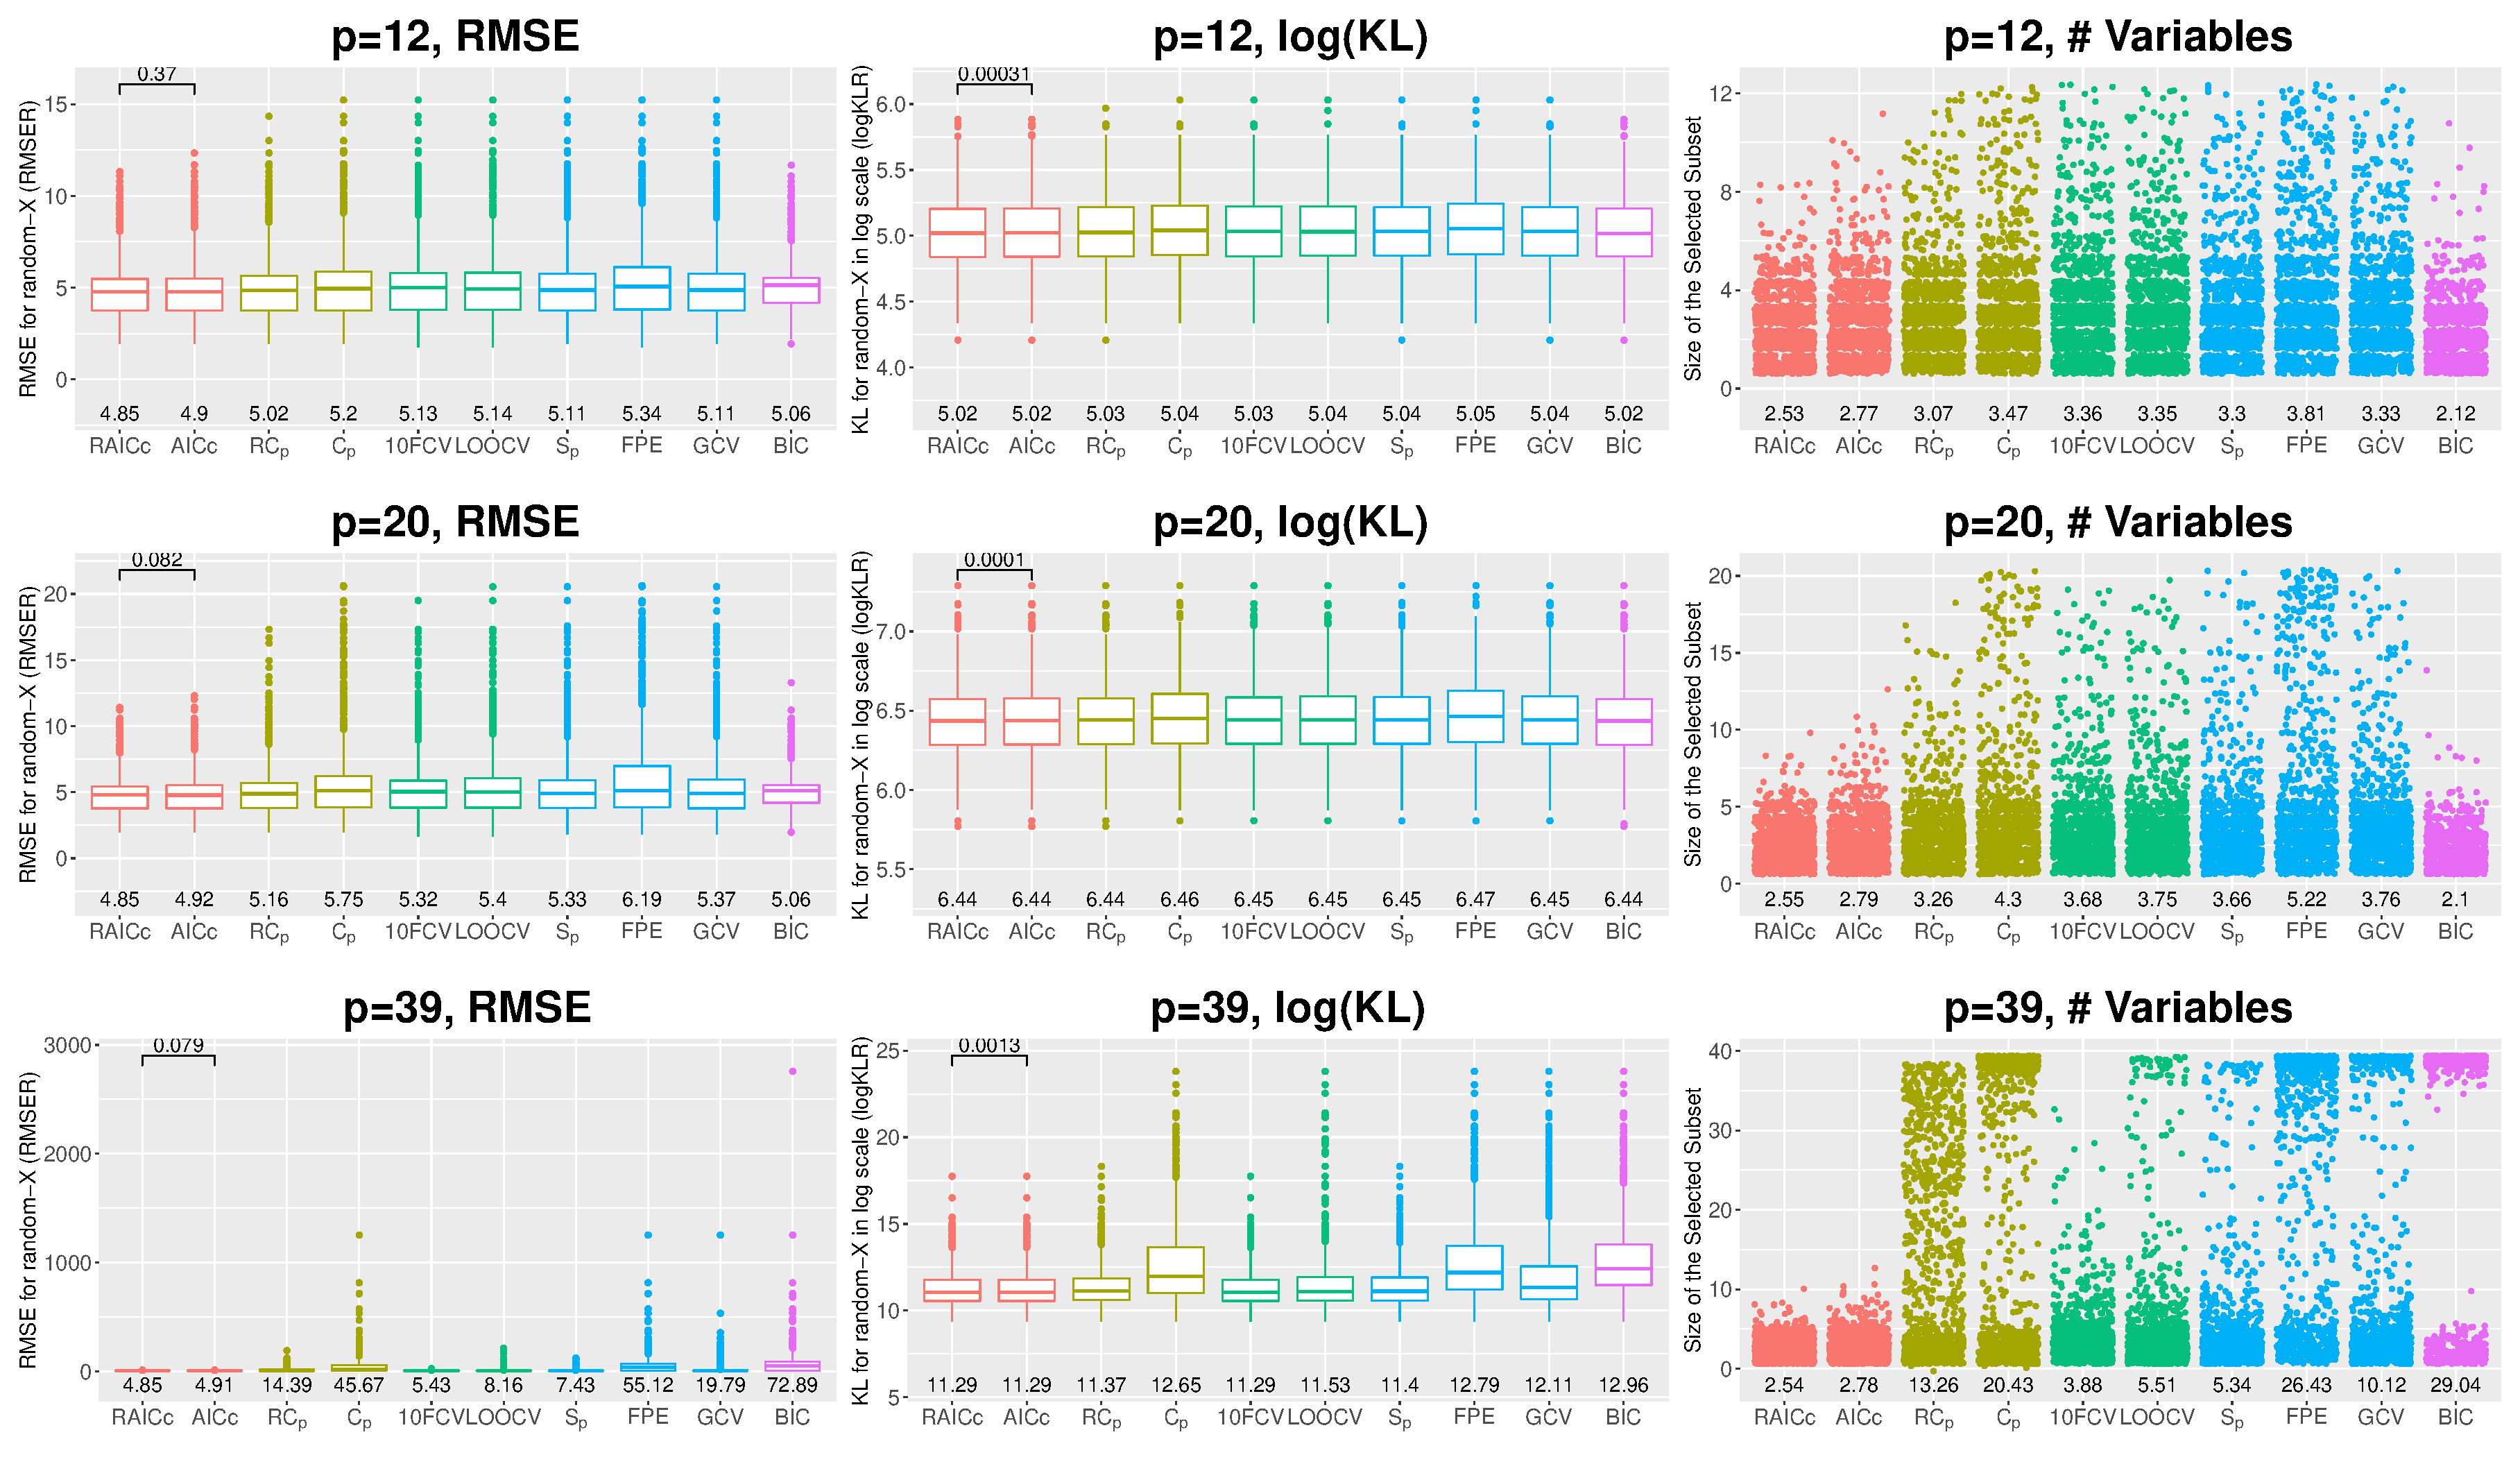
\includegraphics[width=\textwidth]{figures/supplement/randomx_VS-Ex1_n40_msnr_rho09.eps}
\caption{VS-Ex1, $n=40$, medium signal, $\rho=0.9$, and Random-X.}
\end{figure}
\begin{figure}[!ht]
\centering
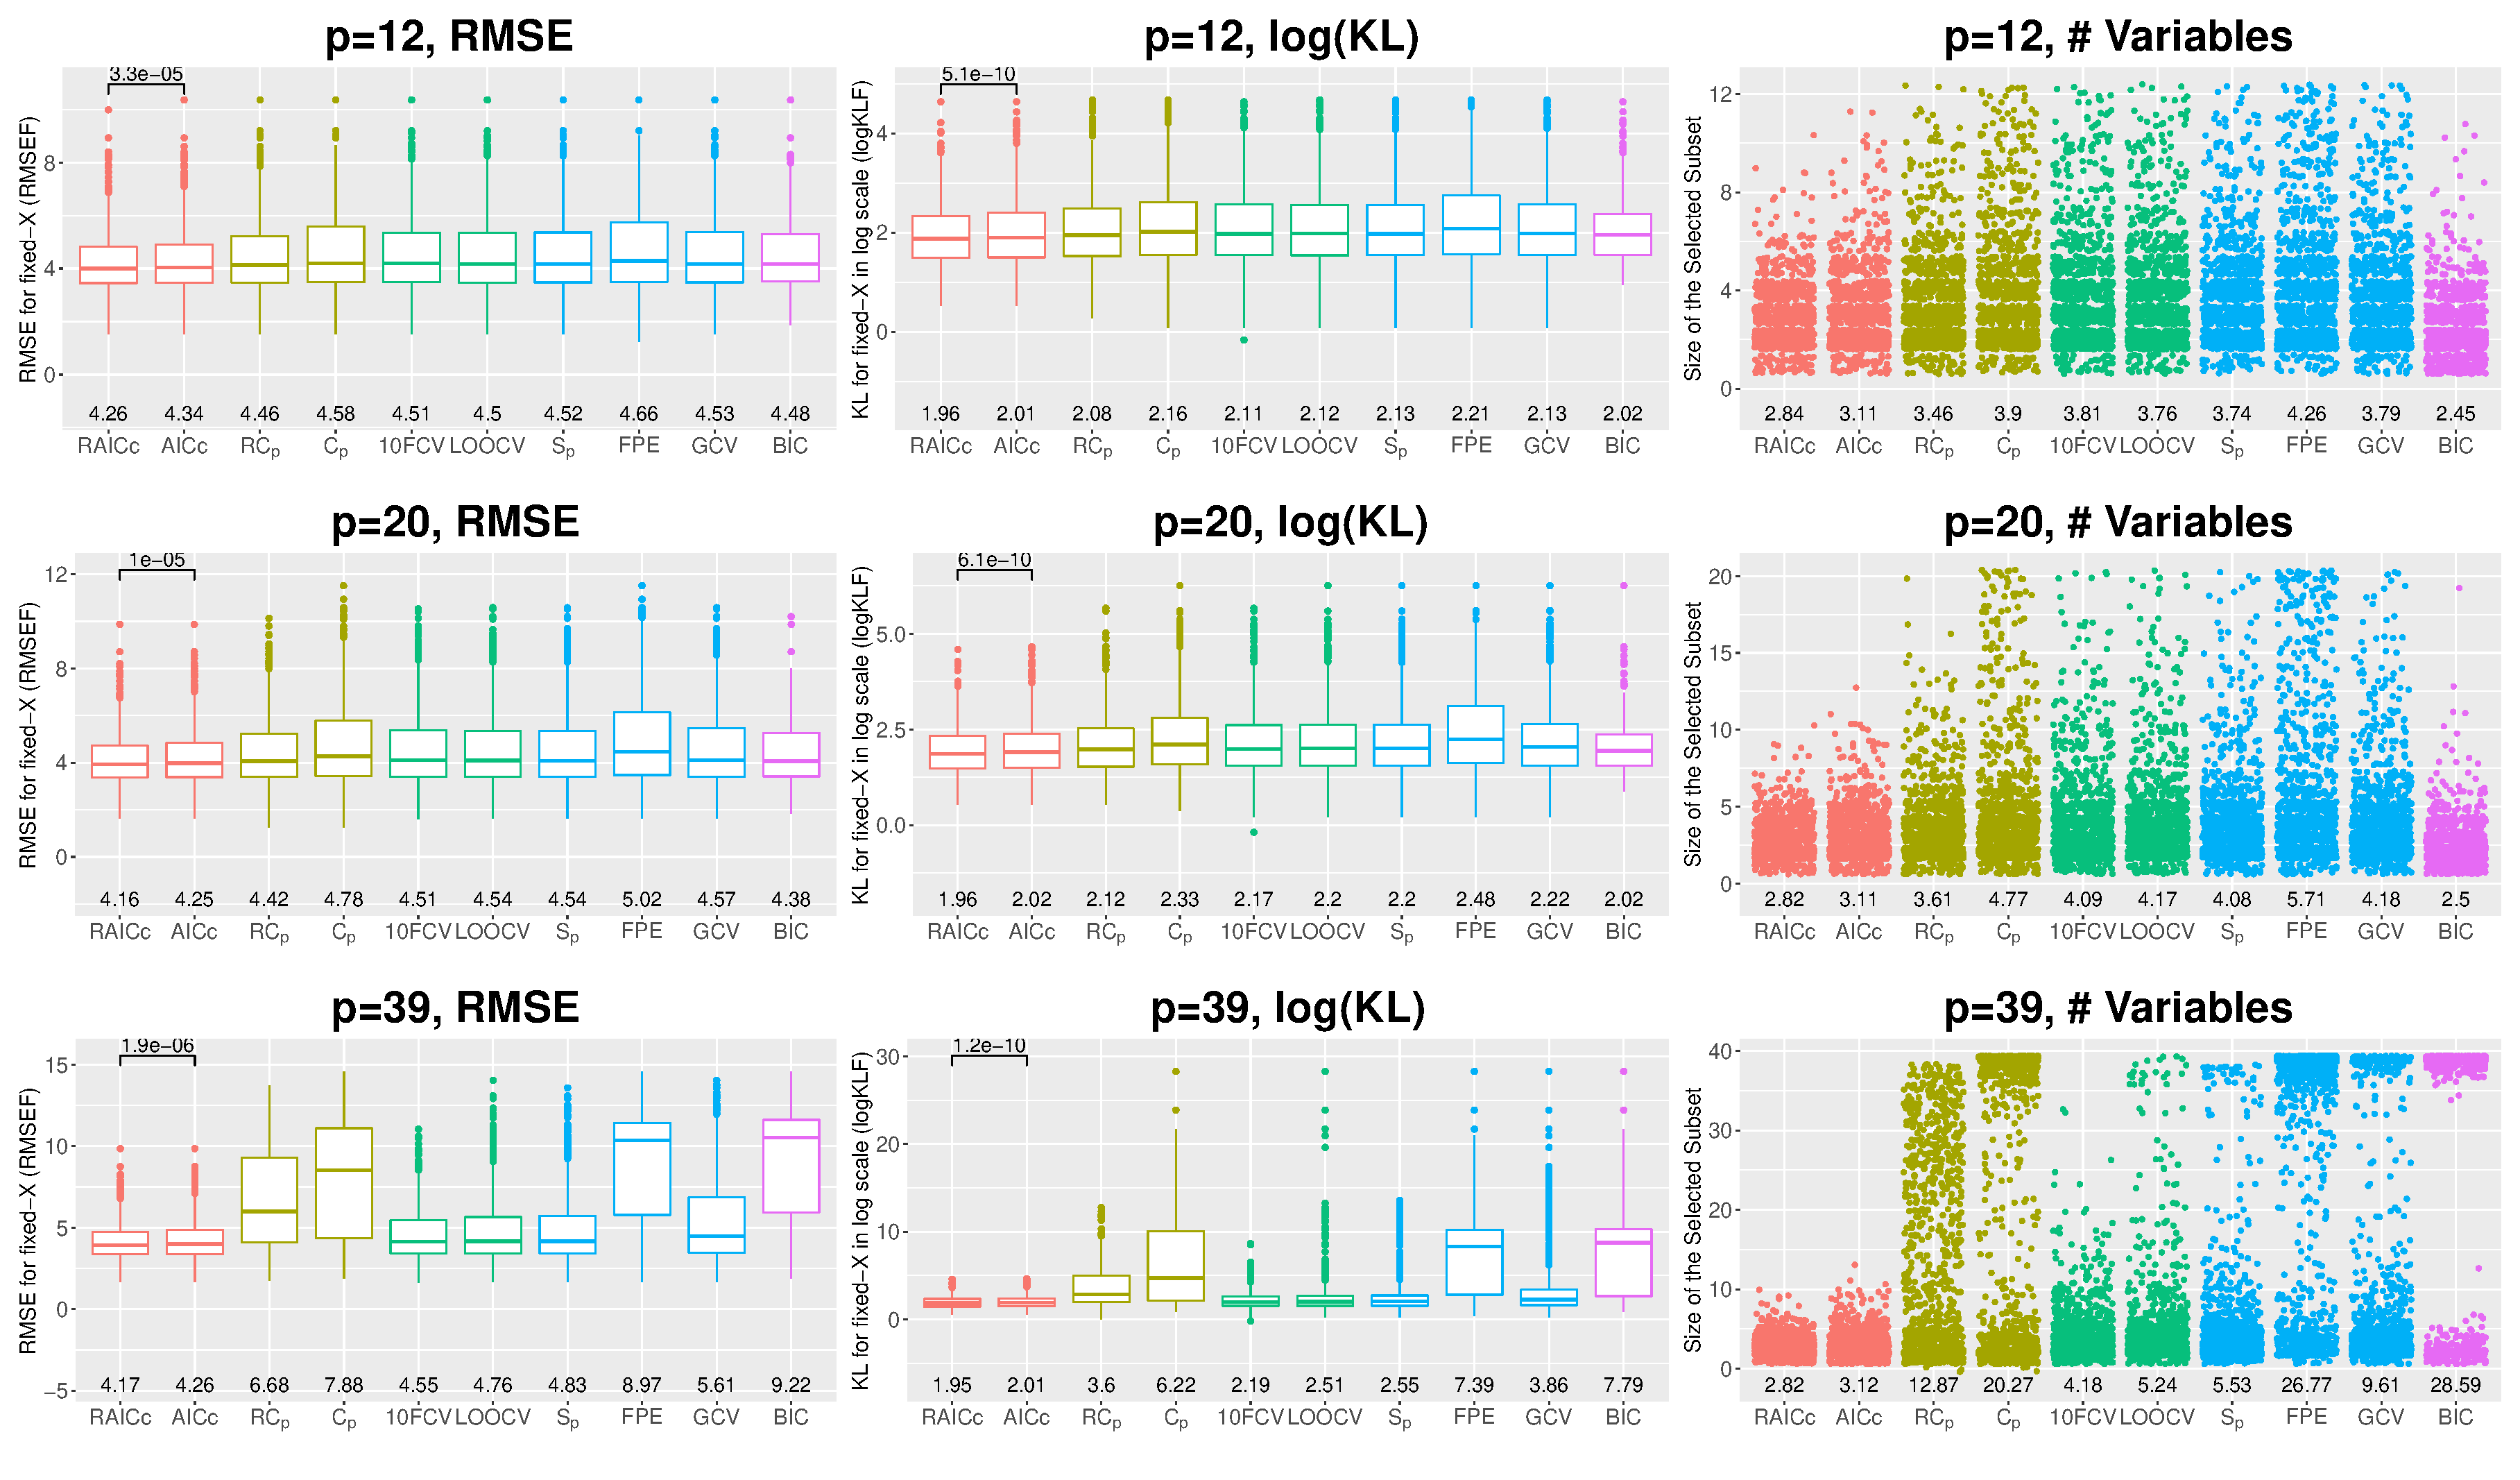
\includegraphics[width=\textwidth]{figures/supplement/fixedx_VS-Ex1_n40_msnr_rho09.eps}
\caption{VS-Ex1, $n=40$, medium signal, $\rho=0.9$, and Fixed-X.}
\end{figure}
\clearpage
\begin{figure}[!ht]
\centering
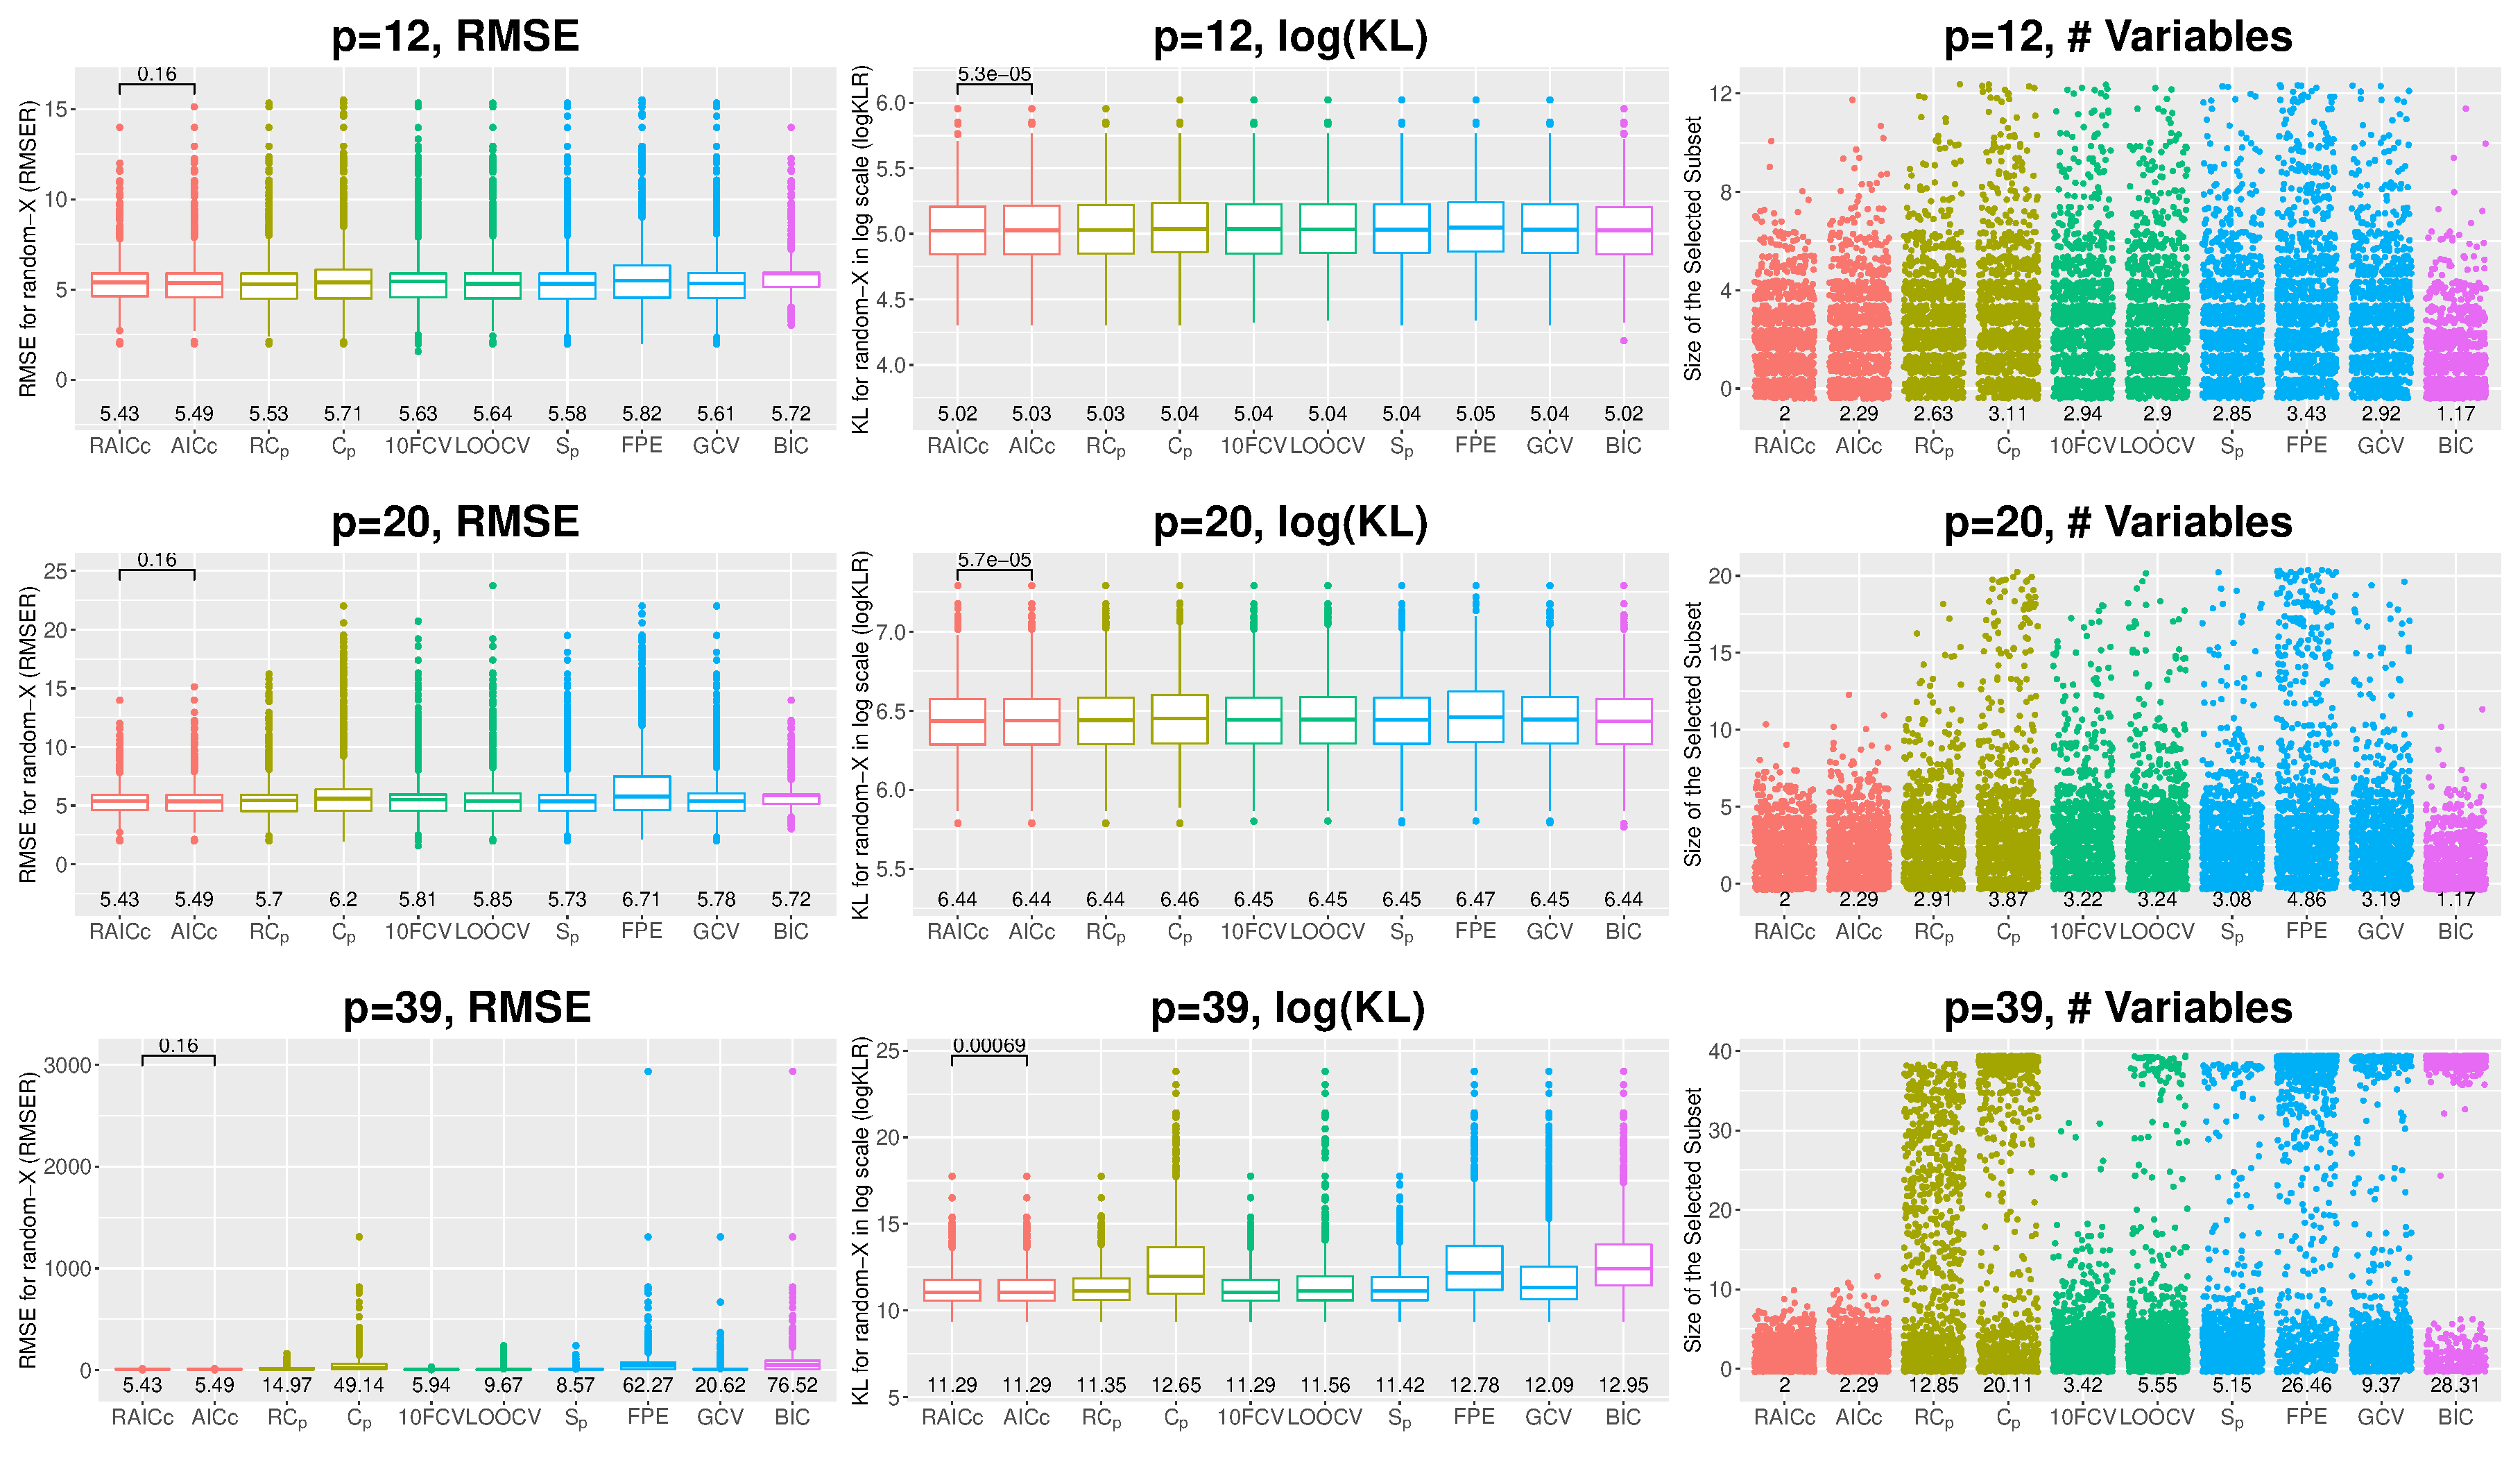
\includegraphics[width=\textwidth]{figures/supplement/randomx_VS-Ex1_n40_lsnr_rho0.eps}
\caption{VS-Ex1, $n=40$, low signal, $\rho=0$, and Random-X.}
\end{figure}
\begin{figure}[!ht]
\centering
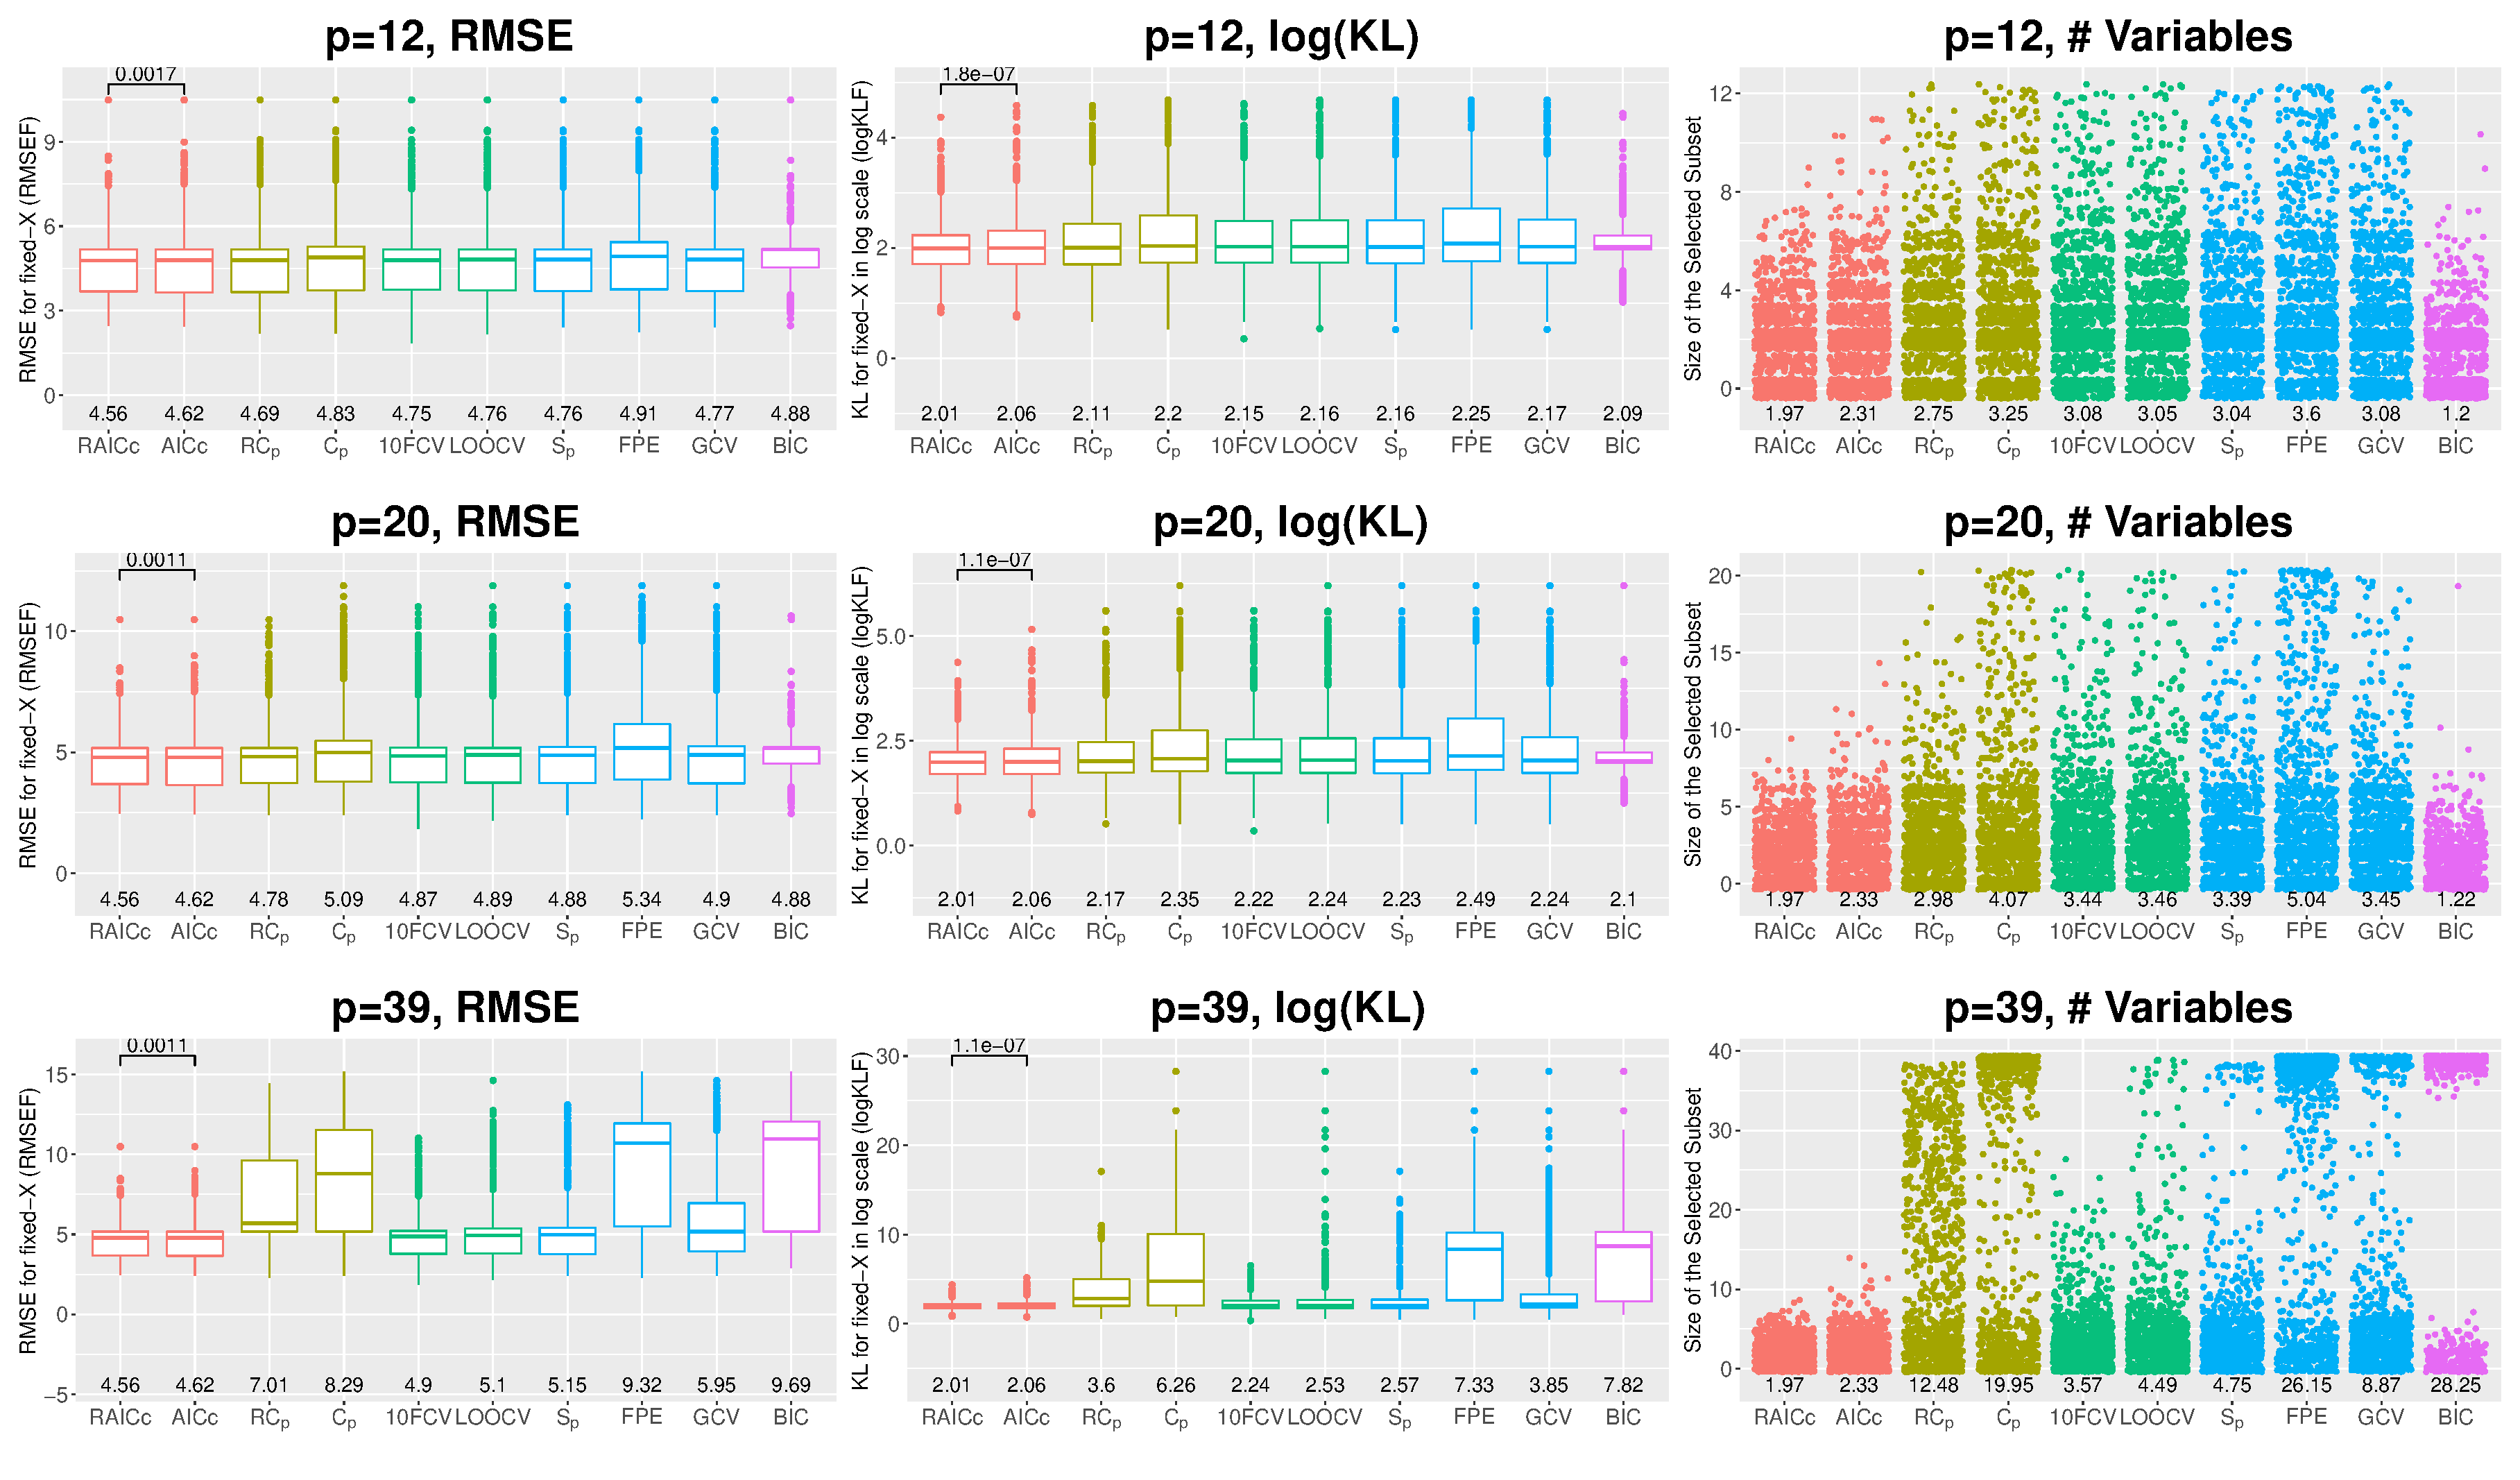
\includegraphics[width=\textwidth]{figures/supplement/fixedx_VS-Ex1_n40_lsnr_rho0.eps}
\caption{VS-Ex1, $n=40$, low signal, $\rho=0$, and Fixed-X.}
\end{figure}
\clearpage
\begin{figure}[!ht]
\centering
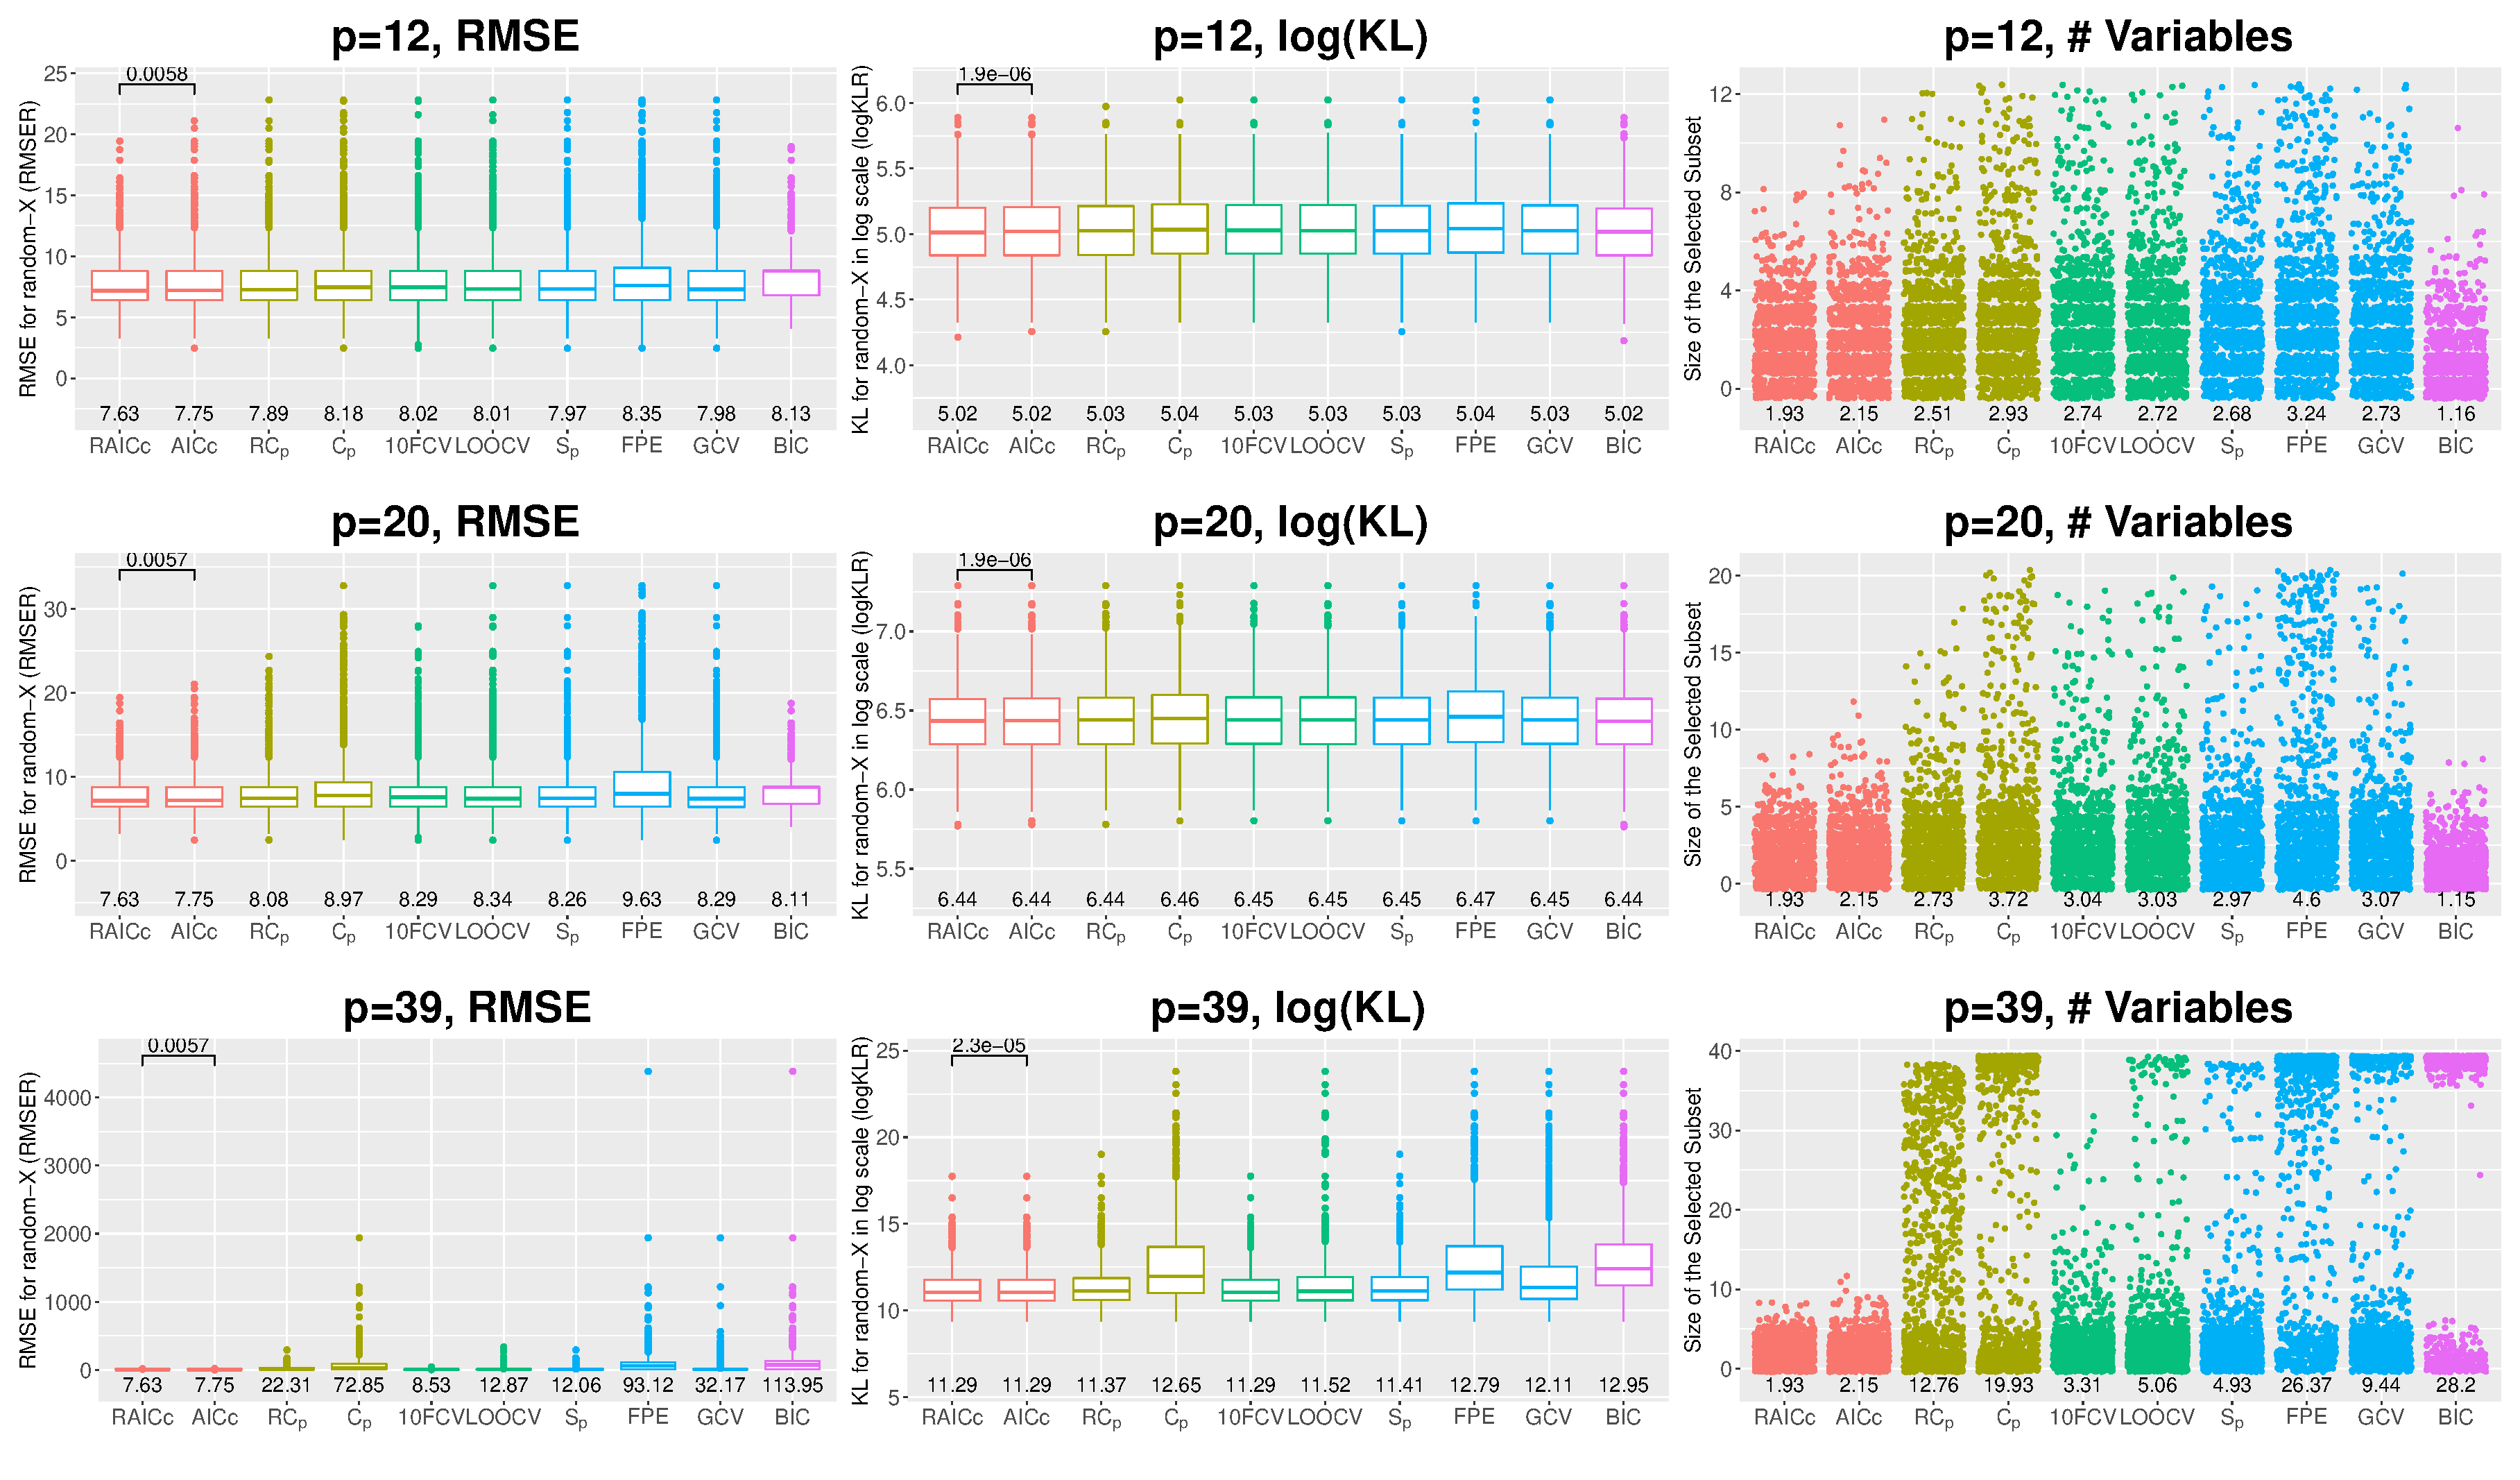
\includegraphics[width=\textwidth]{figures/supplement/randomx_VS-Ex1_n40_lsnr_rho05.eps}
\caption{VS-Ex1, $n=40$, low signal, $\rho=0.5$, and Random-X.}
\end{figure}
\begin{figure}[!ht]
\centering
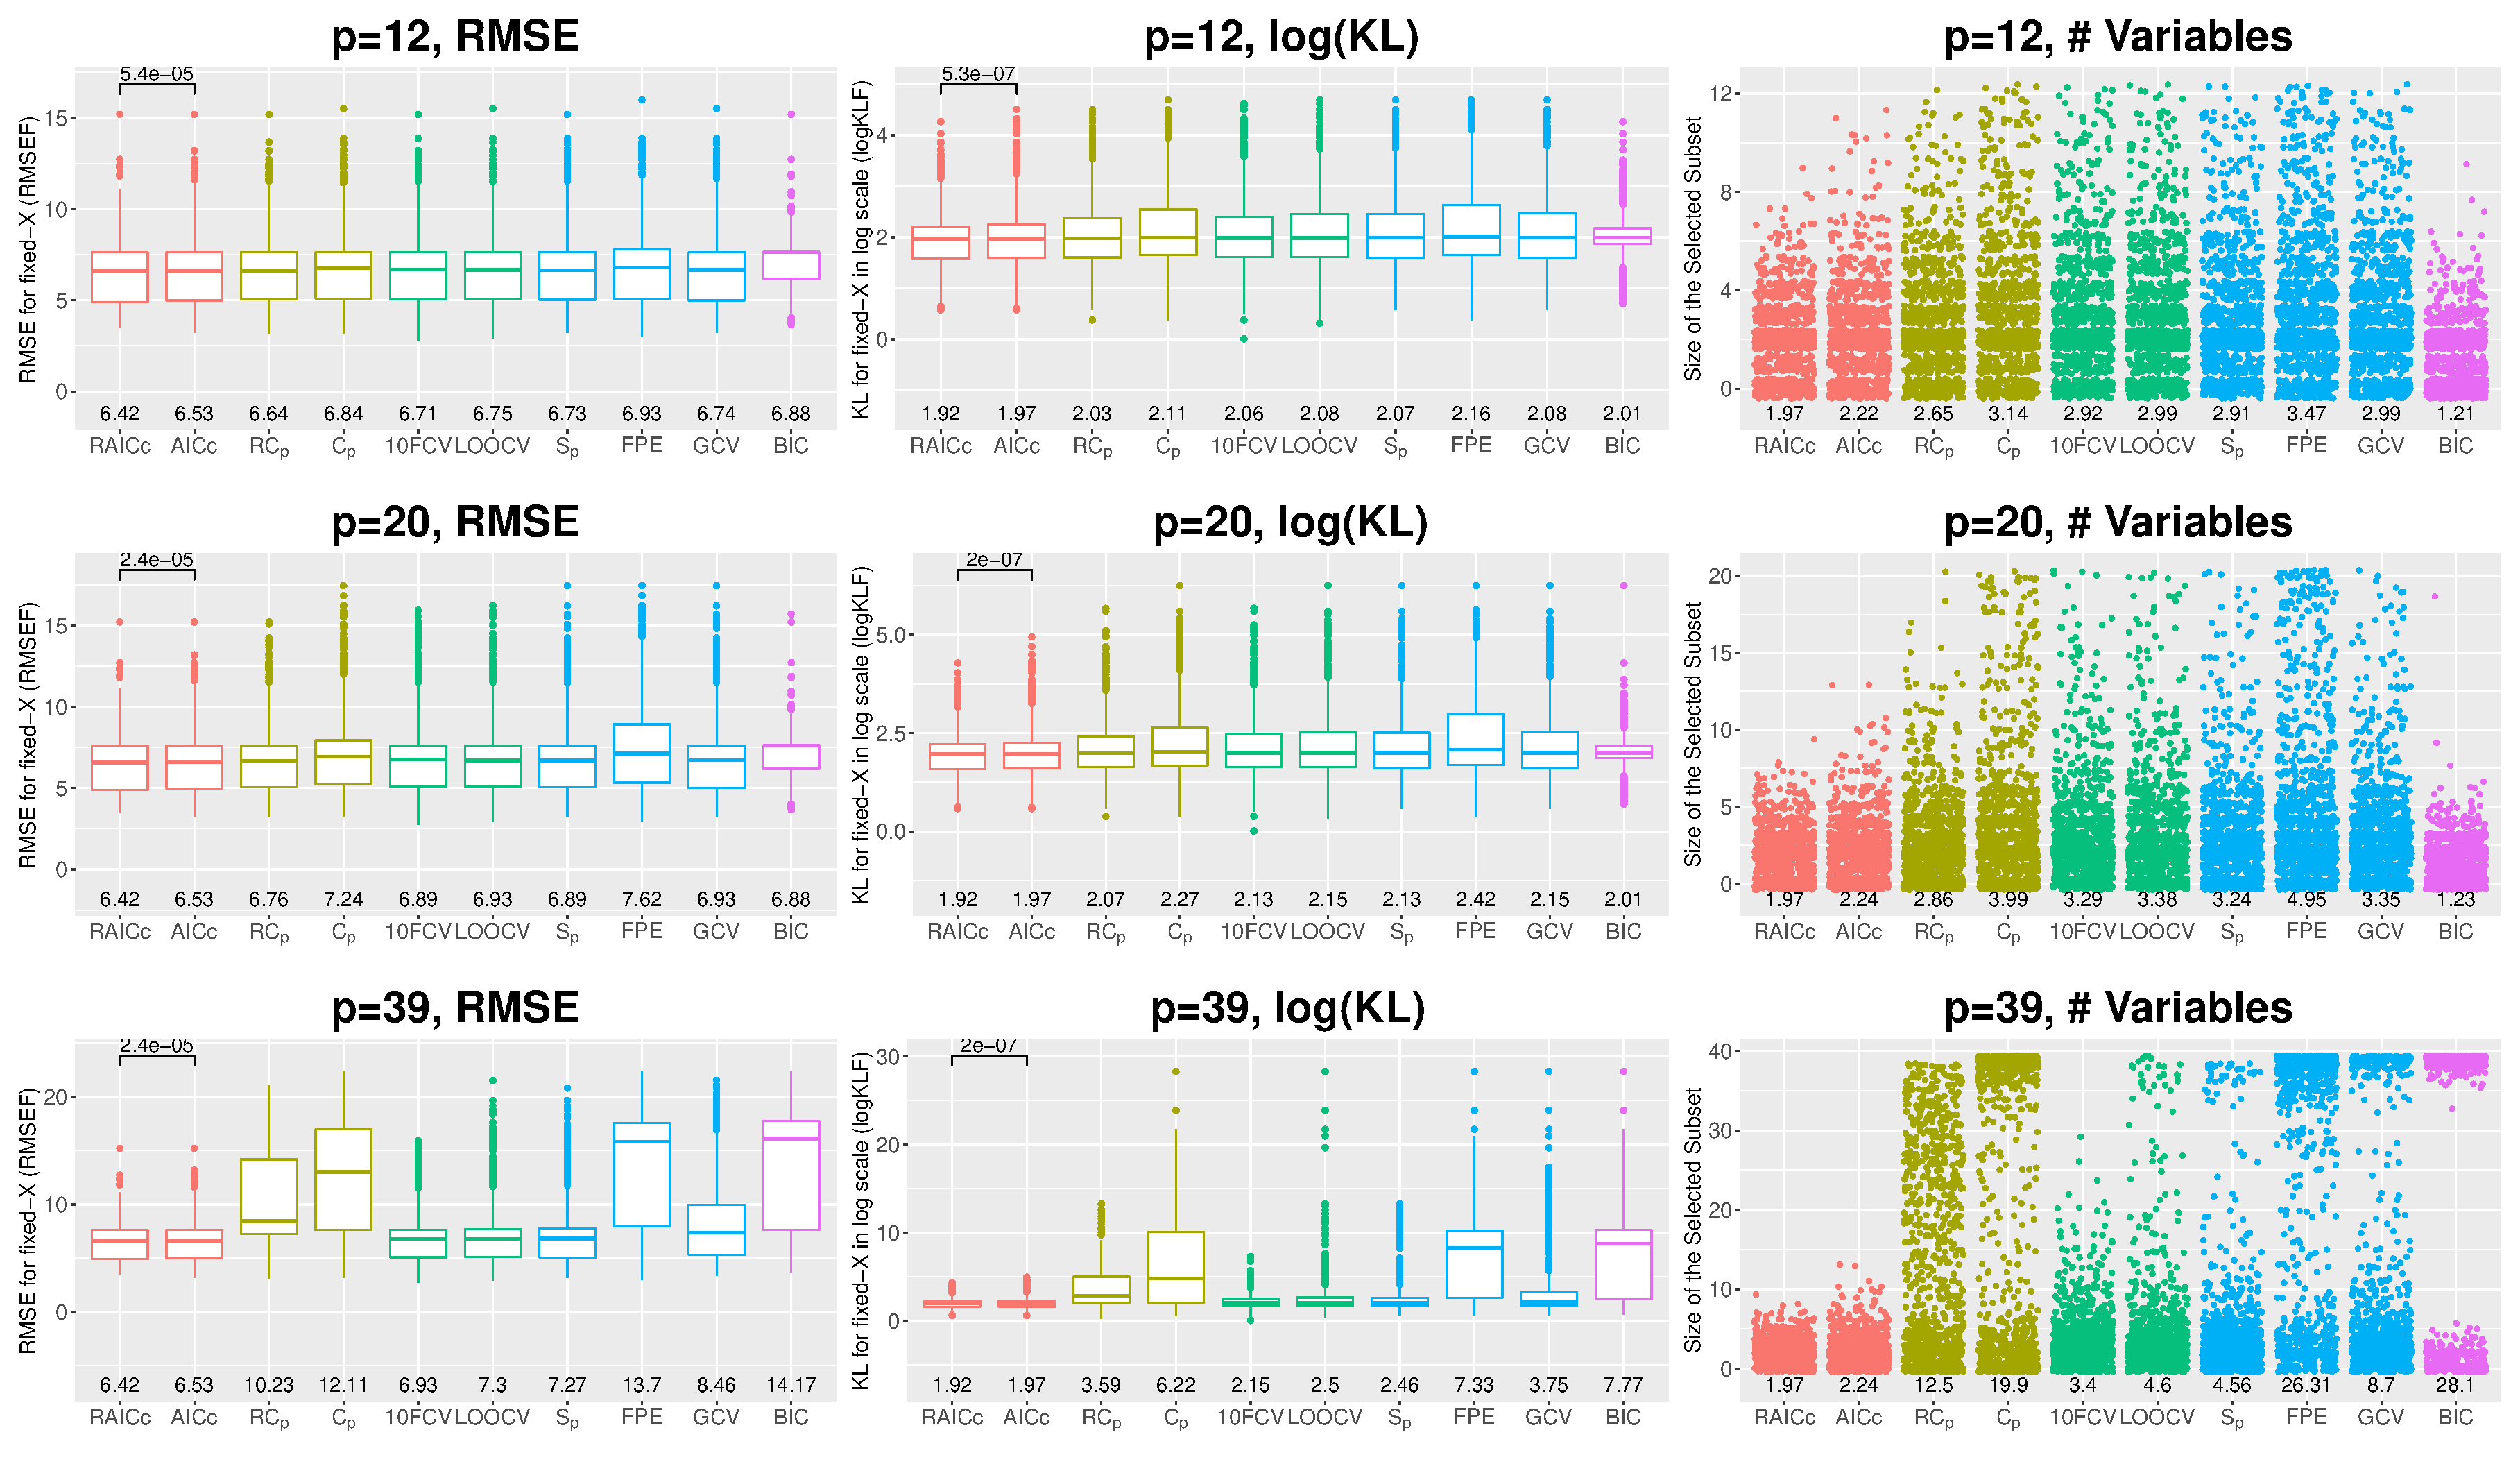
\includegraphics[width=\textwidth]{figures/supplement/fixedx_VS-Ex1_n40_lsnr_rho05.eps}
\caption{VS-Ex1, $n=40$, low signal, $\rho=0.5$, and Fixed-X.}
\end{figure}
\clearpage
\begin{figure}[!ht]
\centering
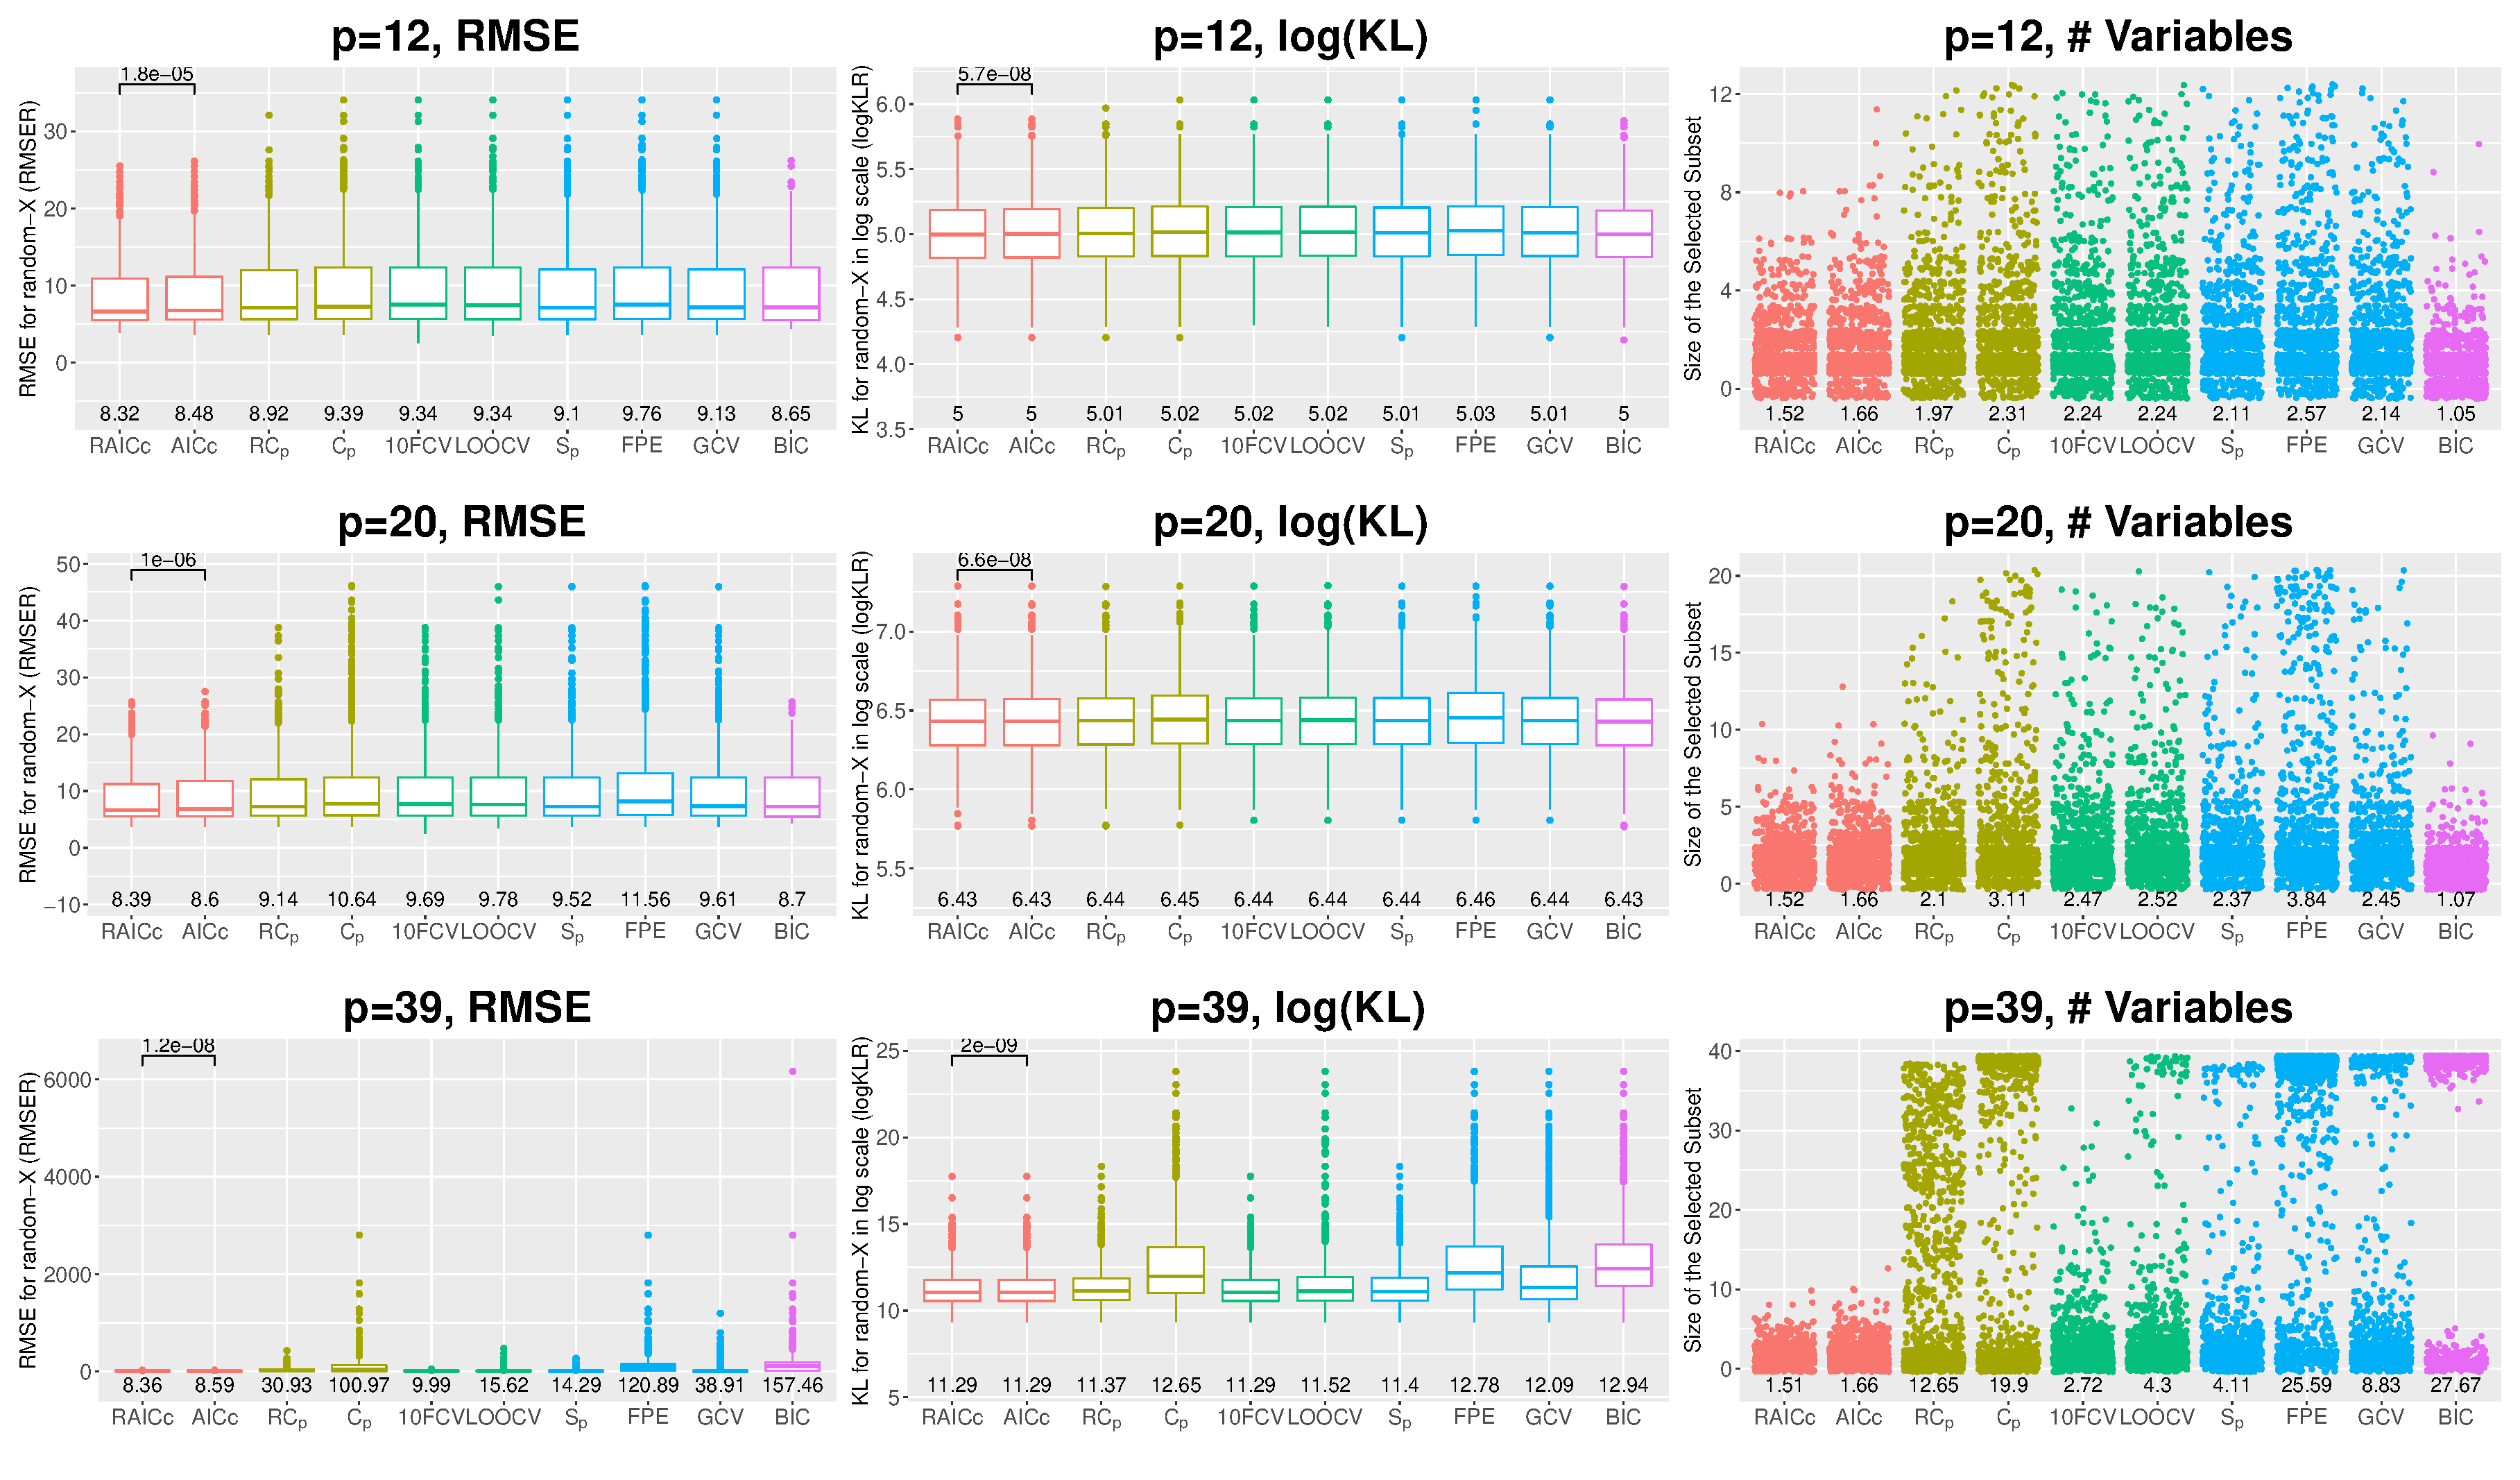
\includegraphics[width=\textwidth]{figures/supplement/randomx_VS-Ex1_n40_lsnr_rho09.eps}
\caption{VS-Ex1, $n=40$, low signal, $\rho=0.9$, and Random-X.}
\end{figure}
\begin{figure}[!ht]
\centering
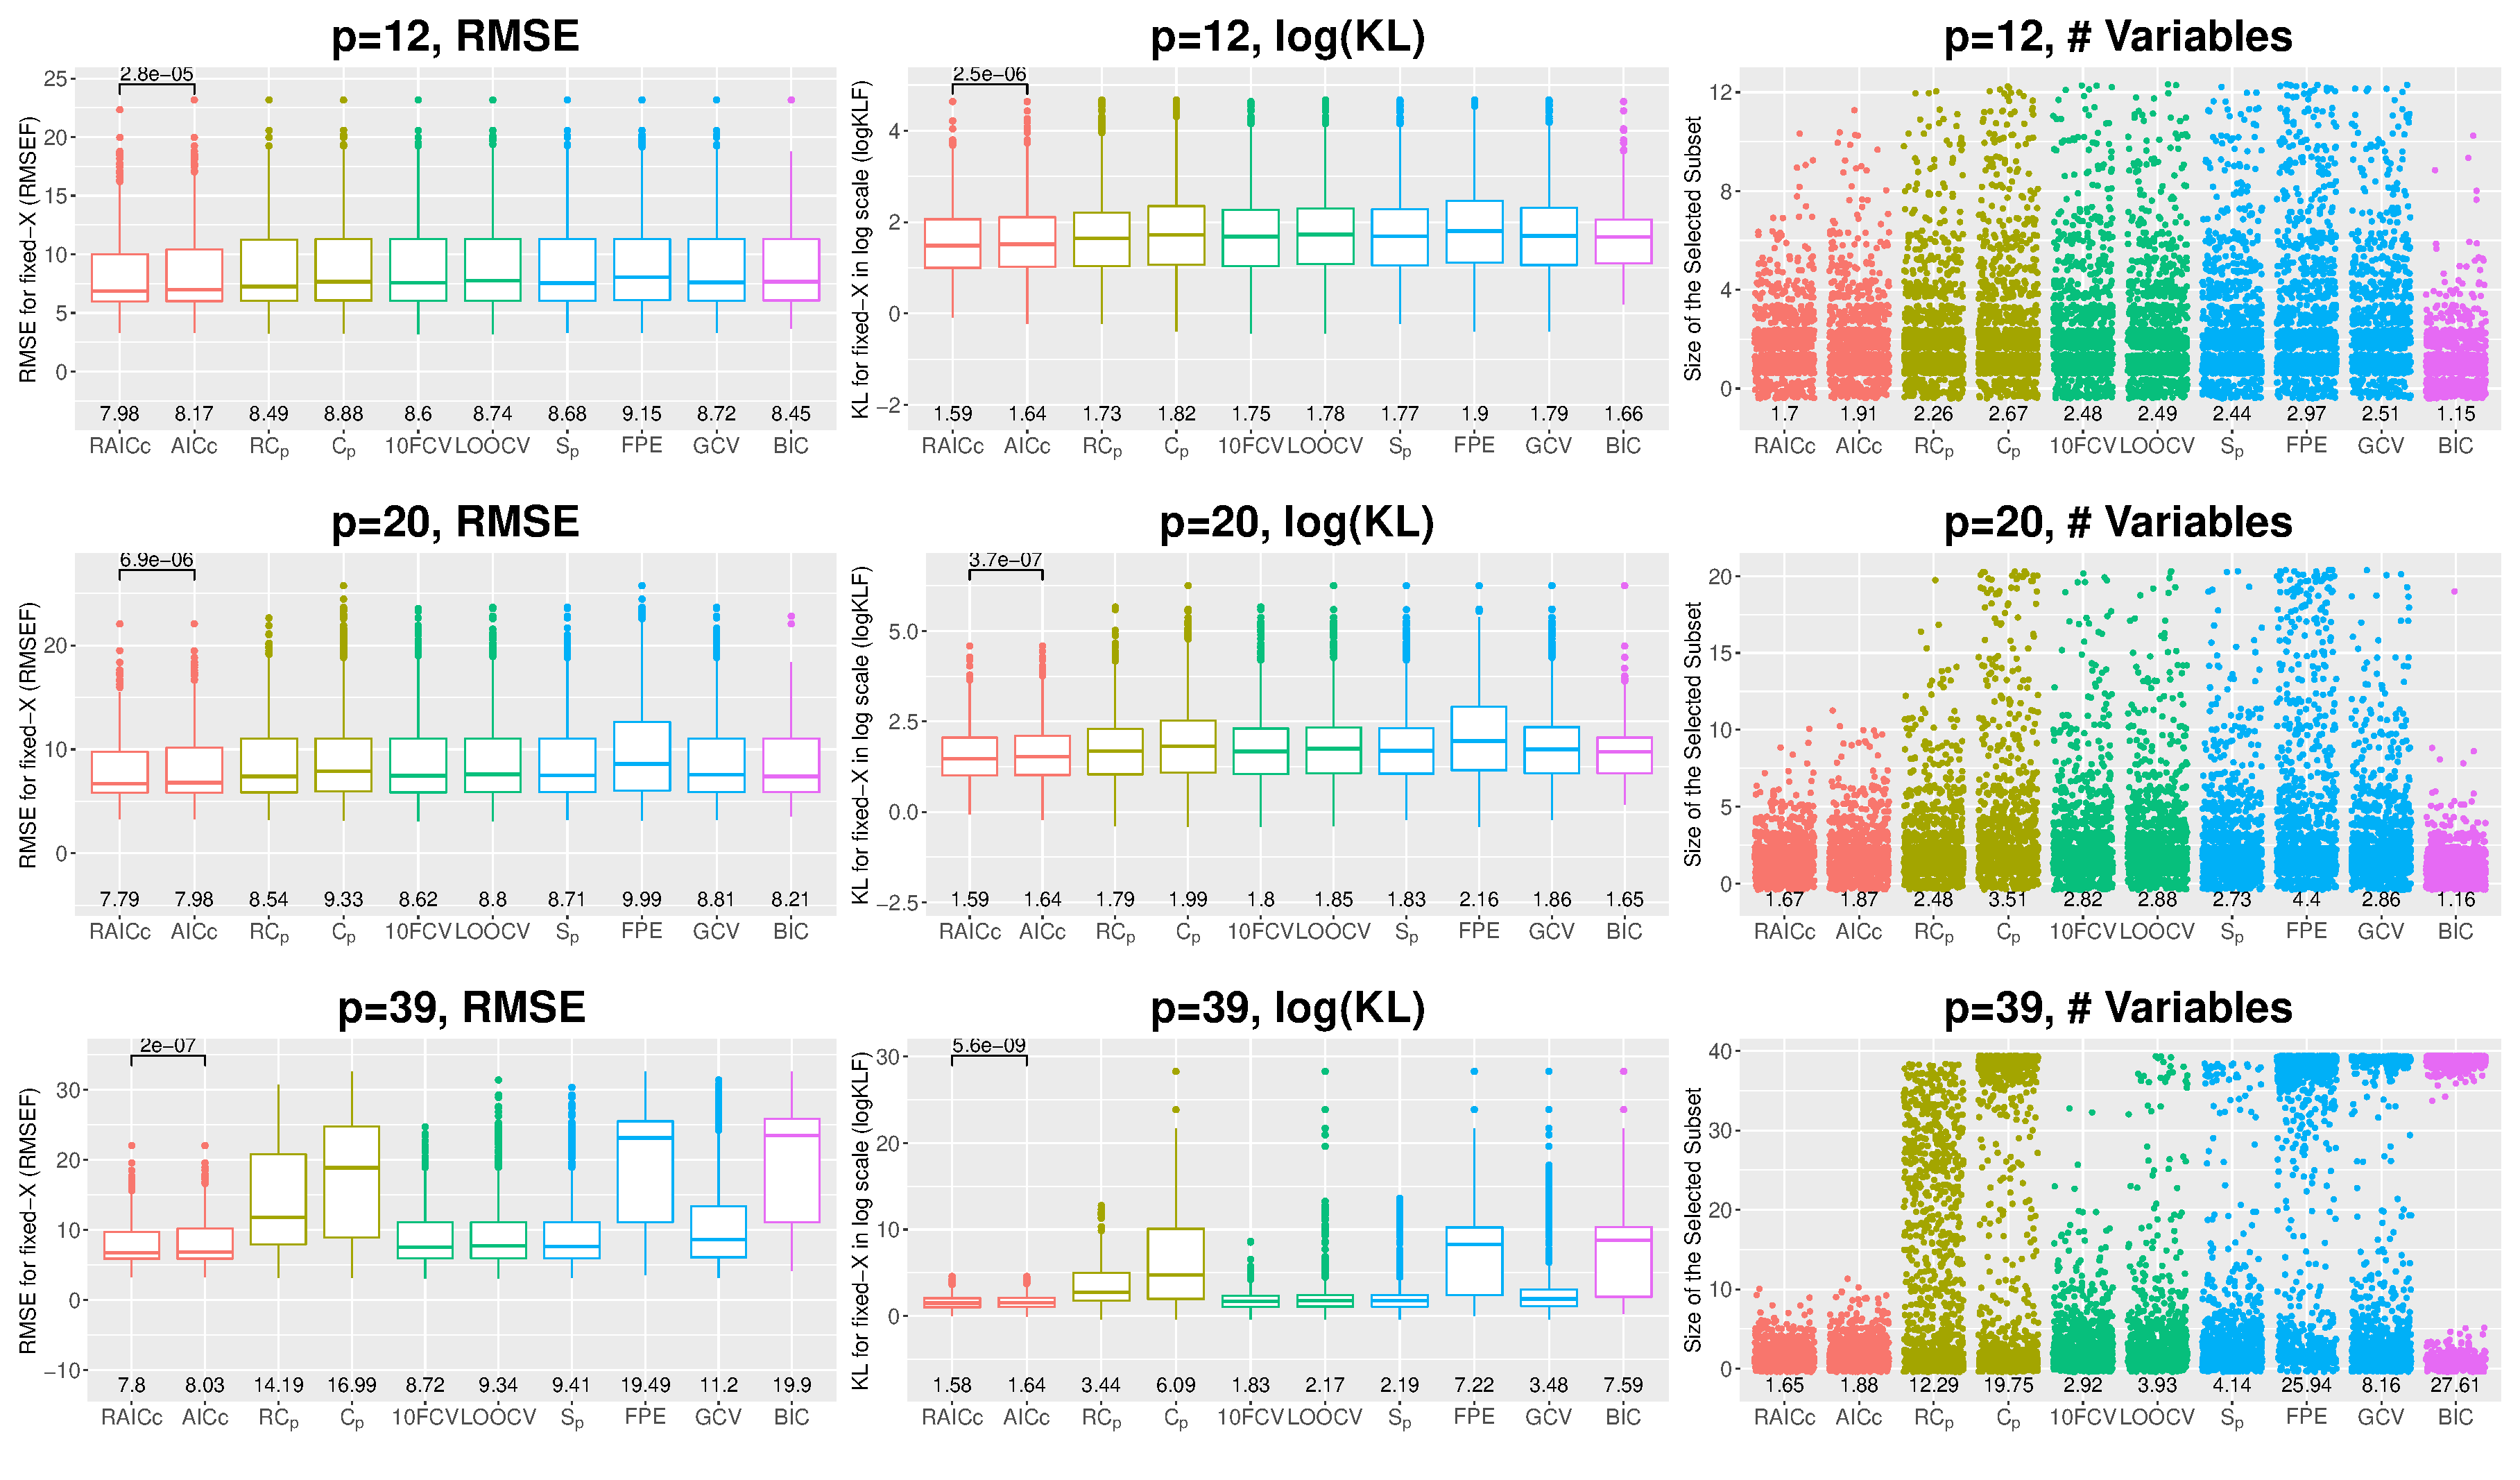
\includegraphics[width=\textwidth]{figures/supplement/fixedx_VS-Ex1_n40_lsnr_rho09.eps}
\caption{VS-Ex1, $n=40$, low signal, $\rho=0.9$, and Fixed-X.}
\end{figure}
\clearpage
\begin{figure}[!ht]
\centering
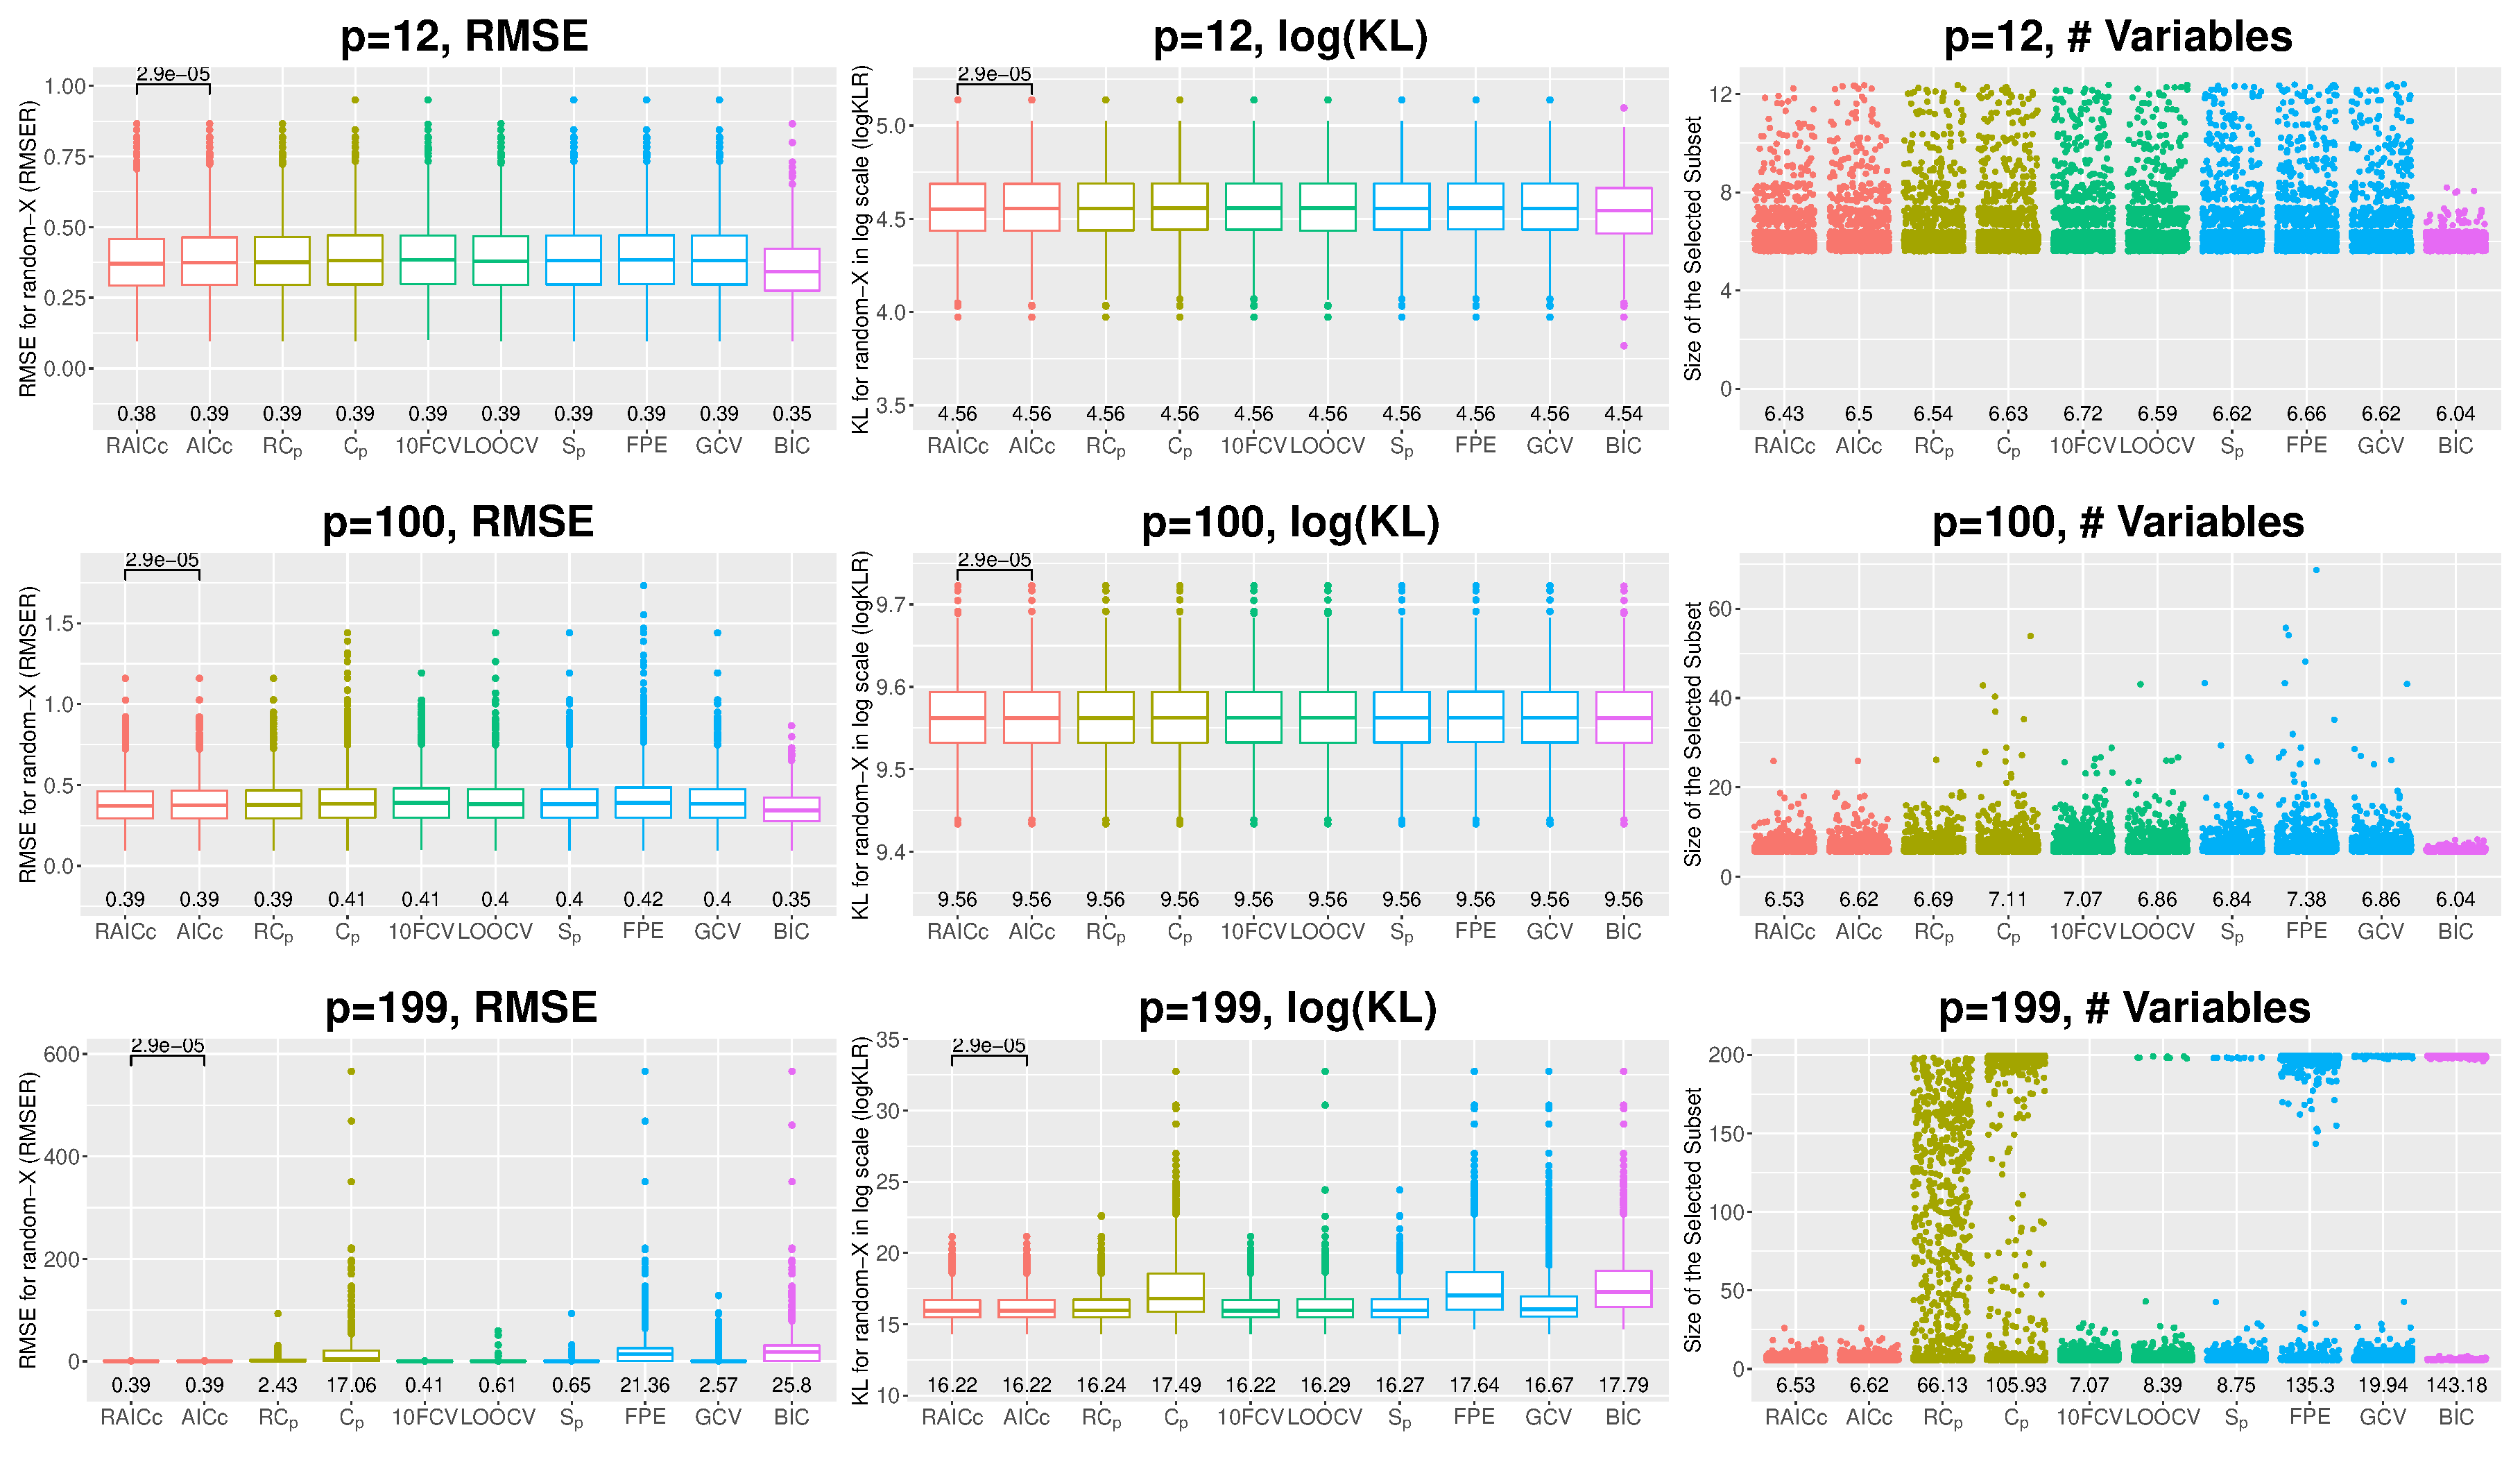
\includegraphics[width=\textwidth]{figures/supplement/randomx_VS-Ex1_n200_hsnr_rho0.eps}
\caption{VS-Ex1, $n=200$, high signal, $\rho=0$, and Random-X.}
\end{figure}
\begin{figure}[!ht]
\centering
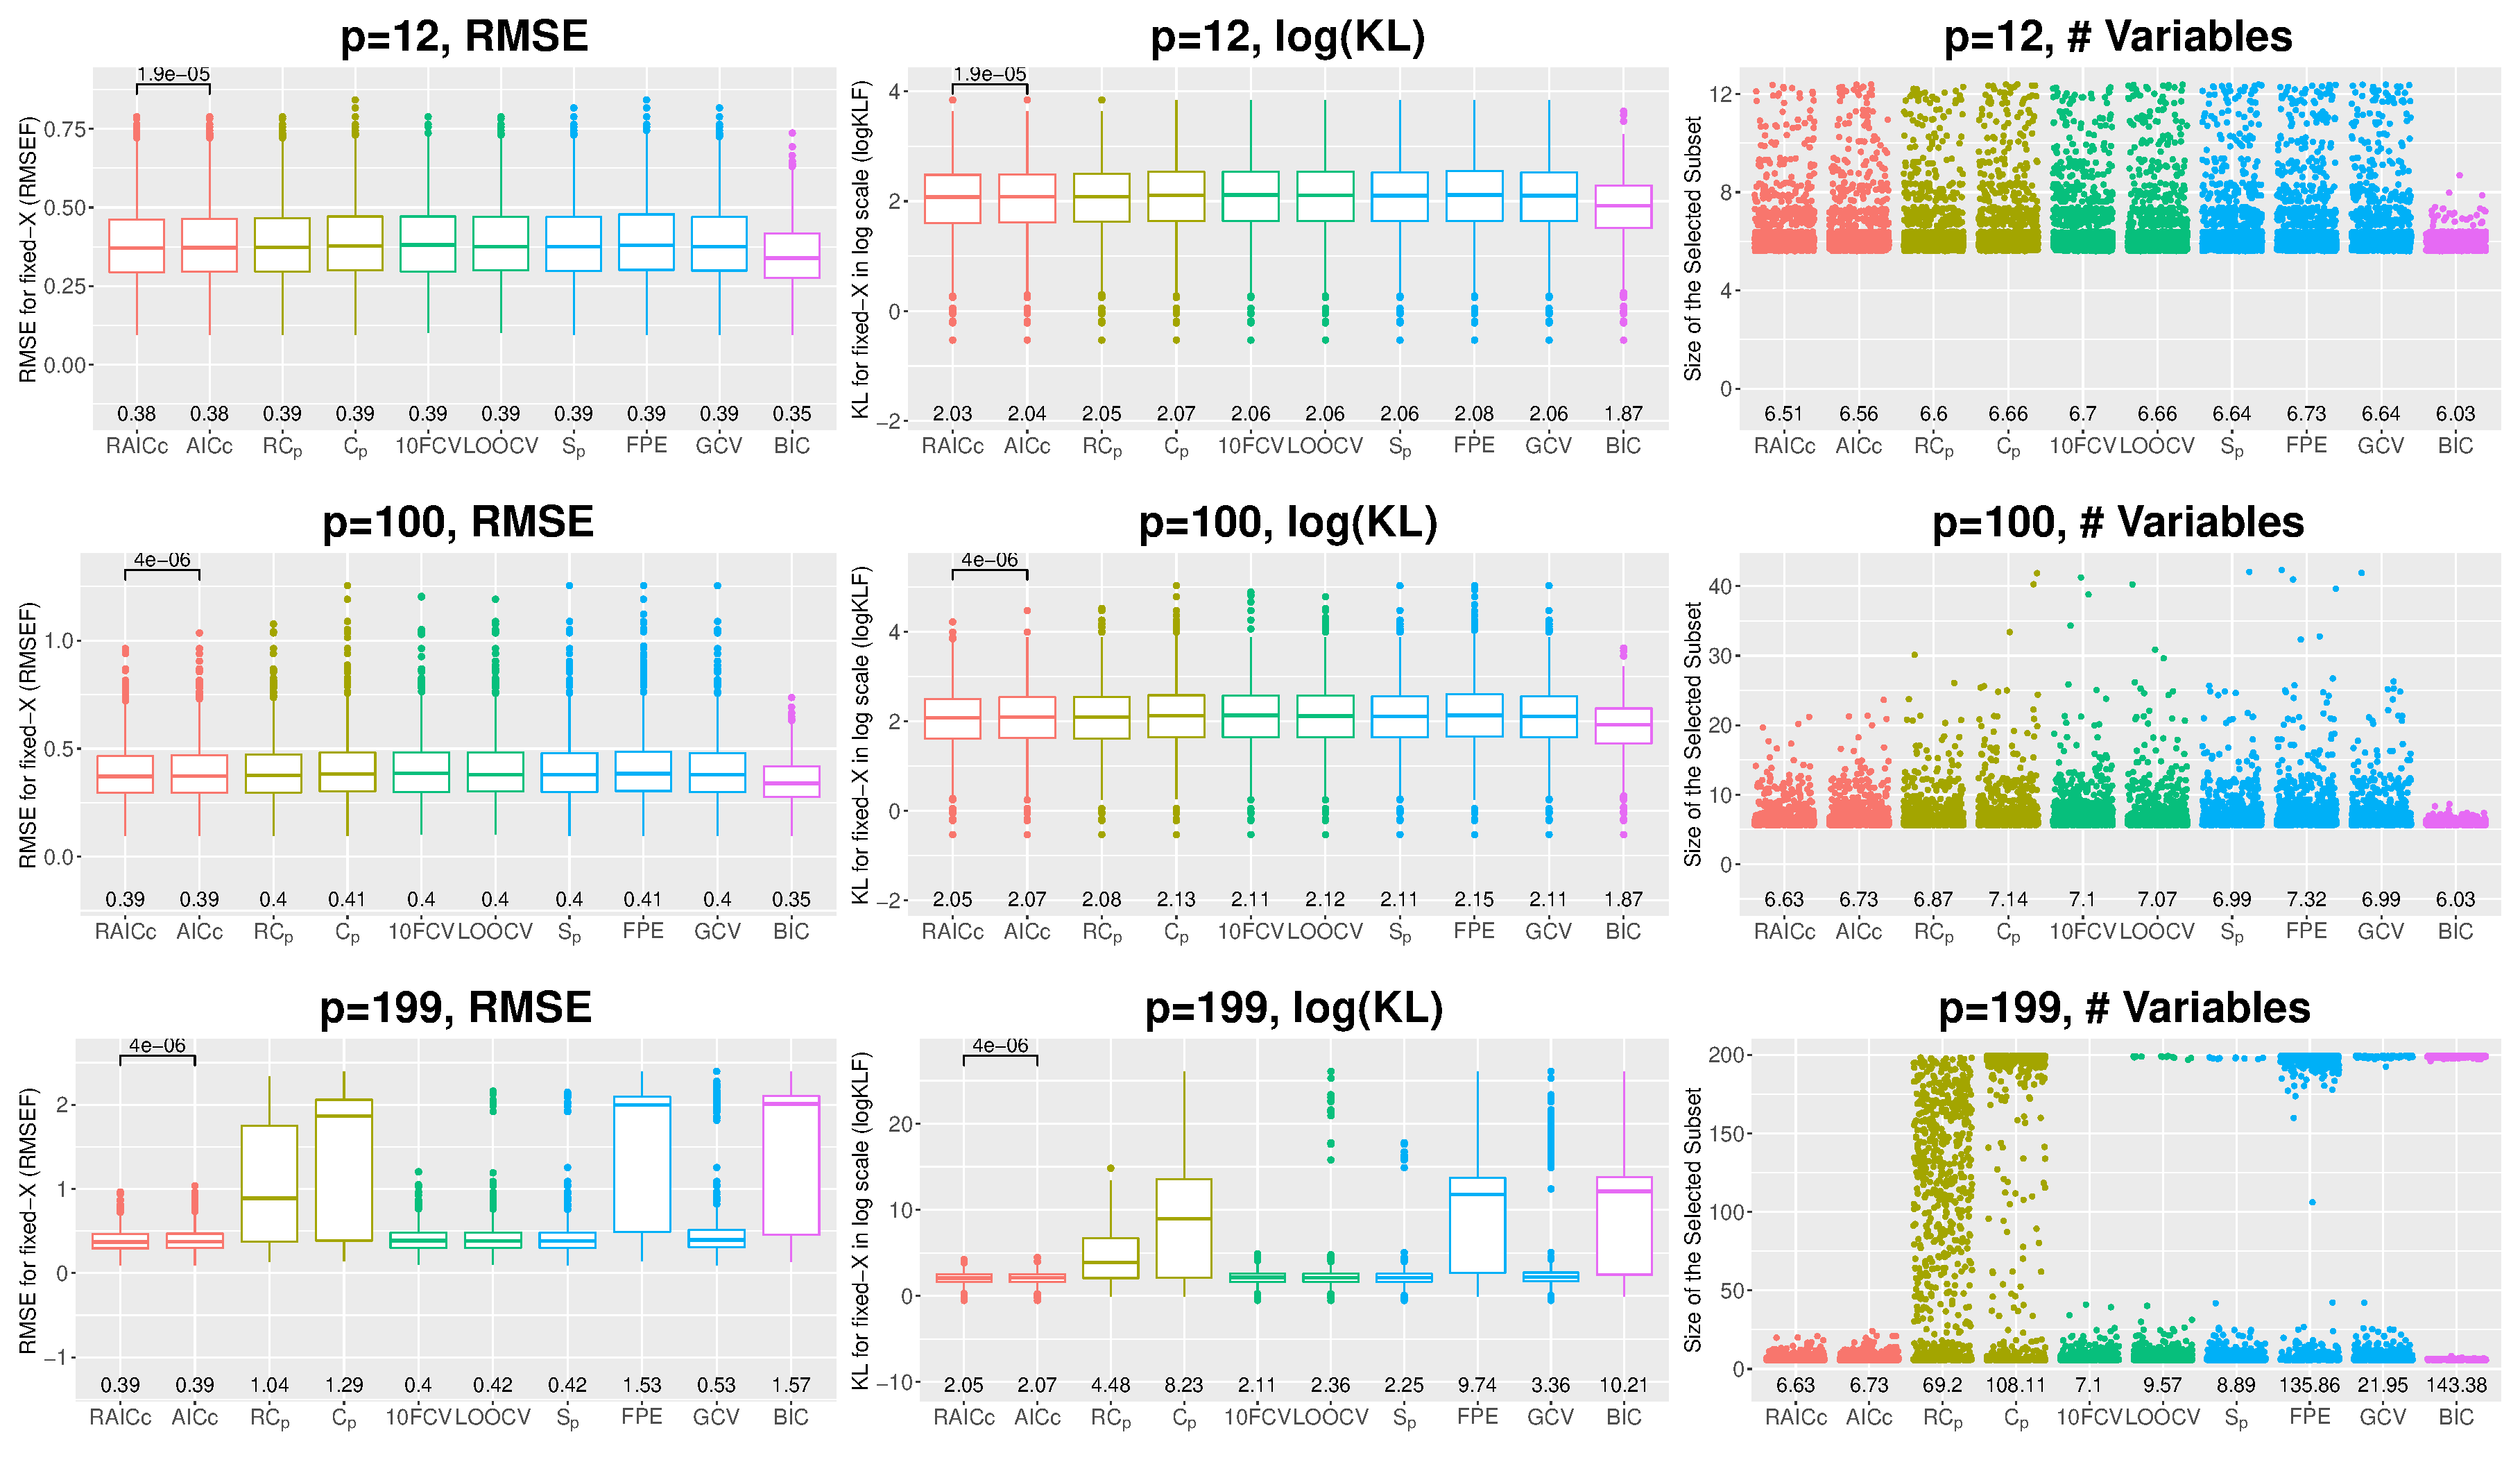
\includegraphics[width=\textwidth]{figures/supplement/fixedx_VS-Ex1_n200_hsnr_rho0.eps}
\caption{VS-Ex1, $n=200$, high signal, $\rho=0$, and Fixed-X.}
\end{figure}
\clearpage
\begin{figure}[!ht]
\centering
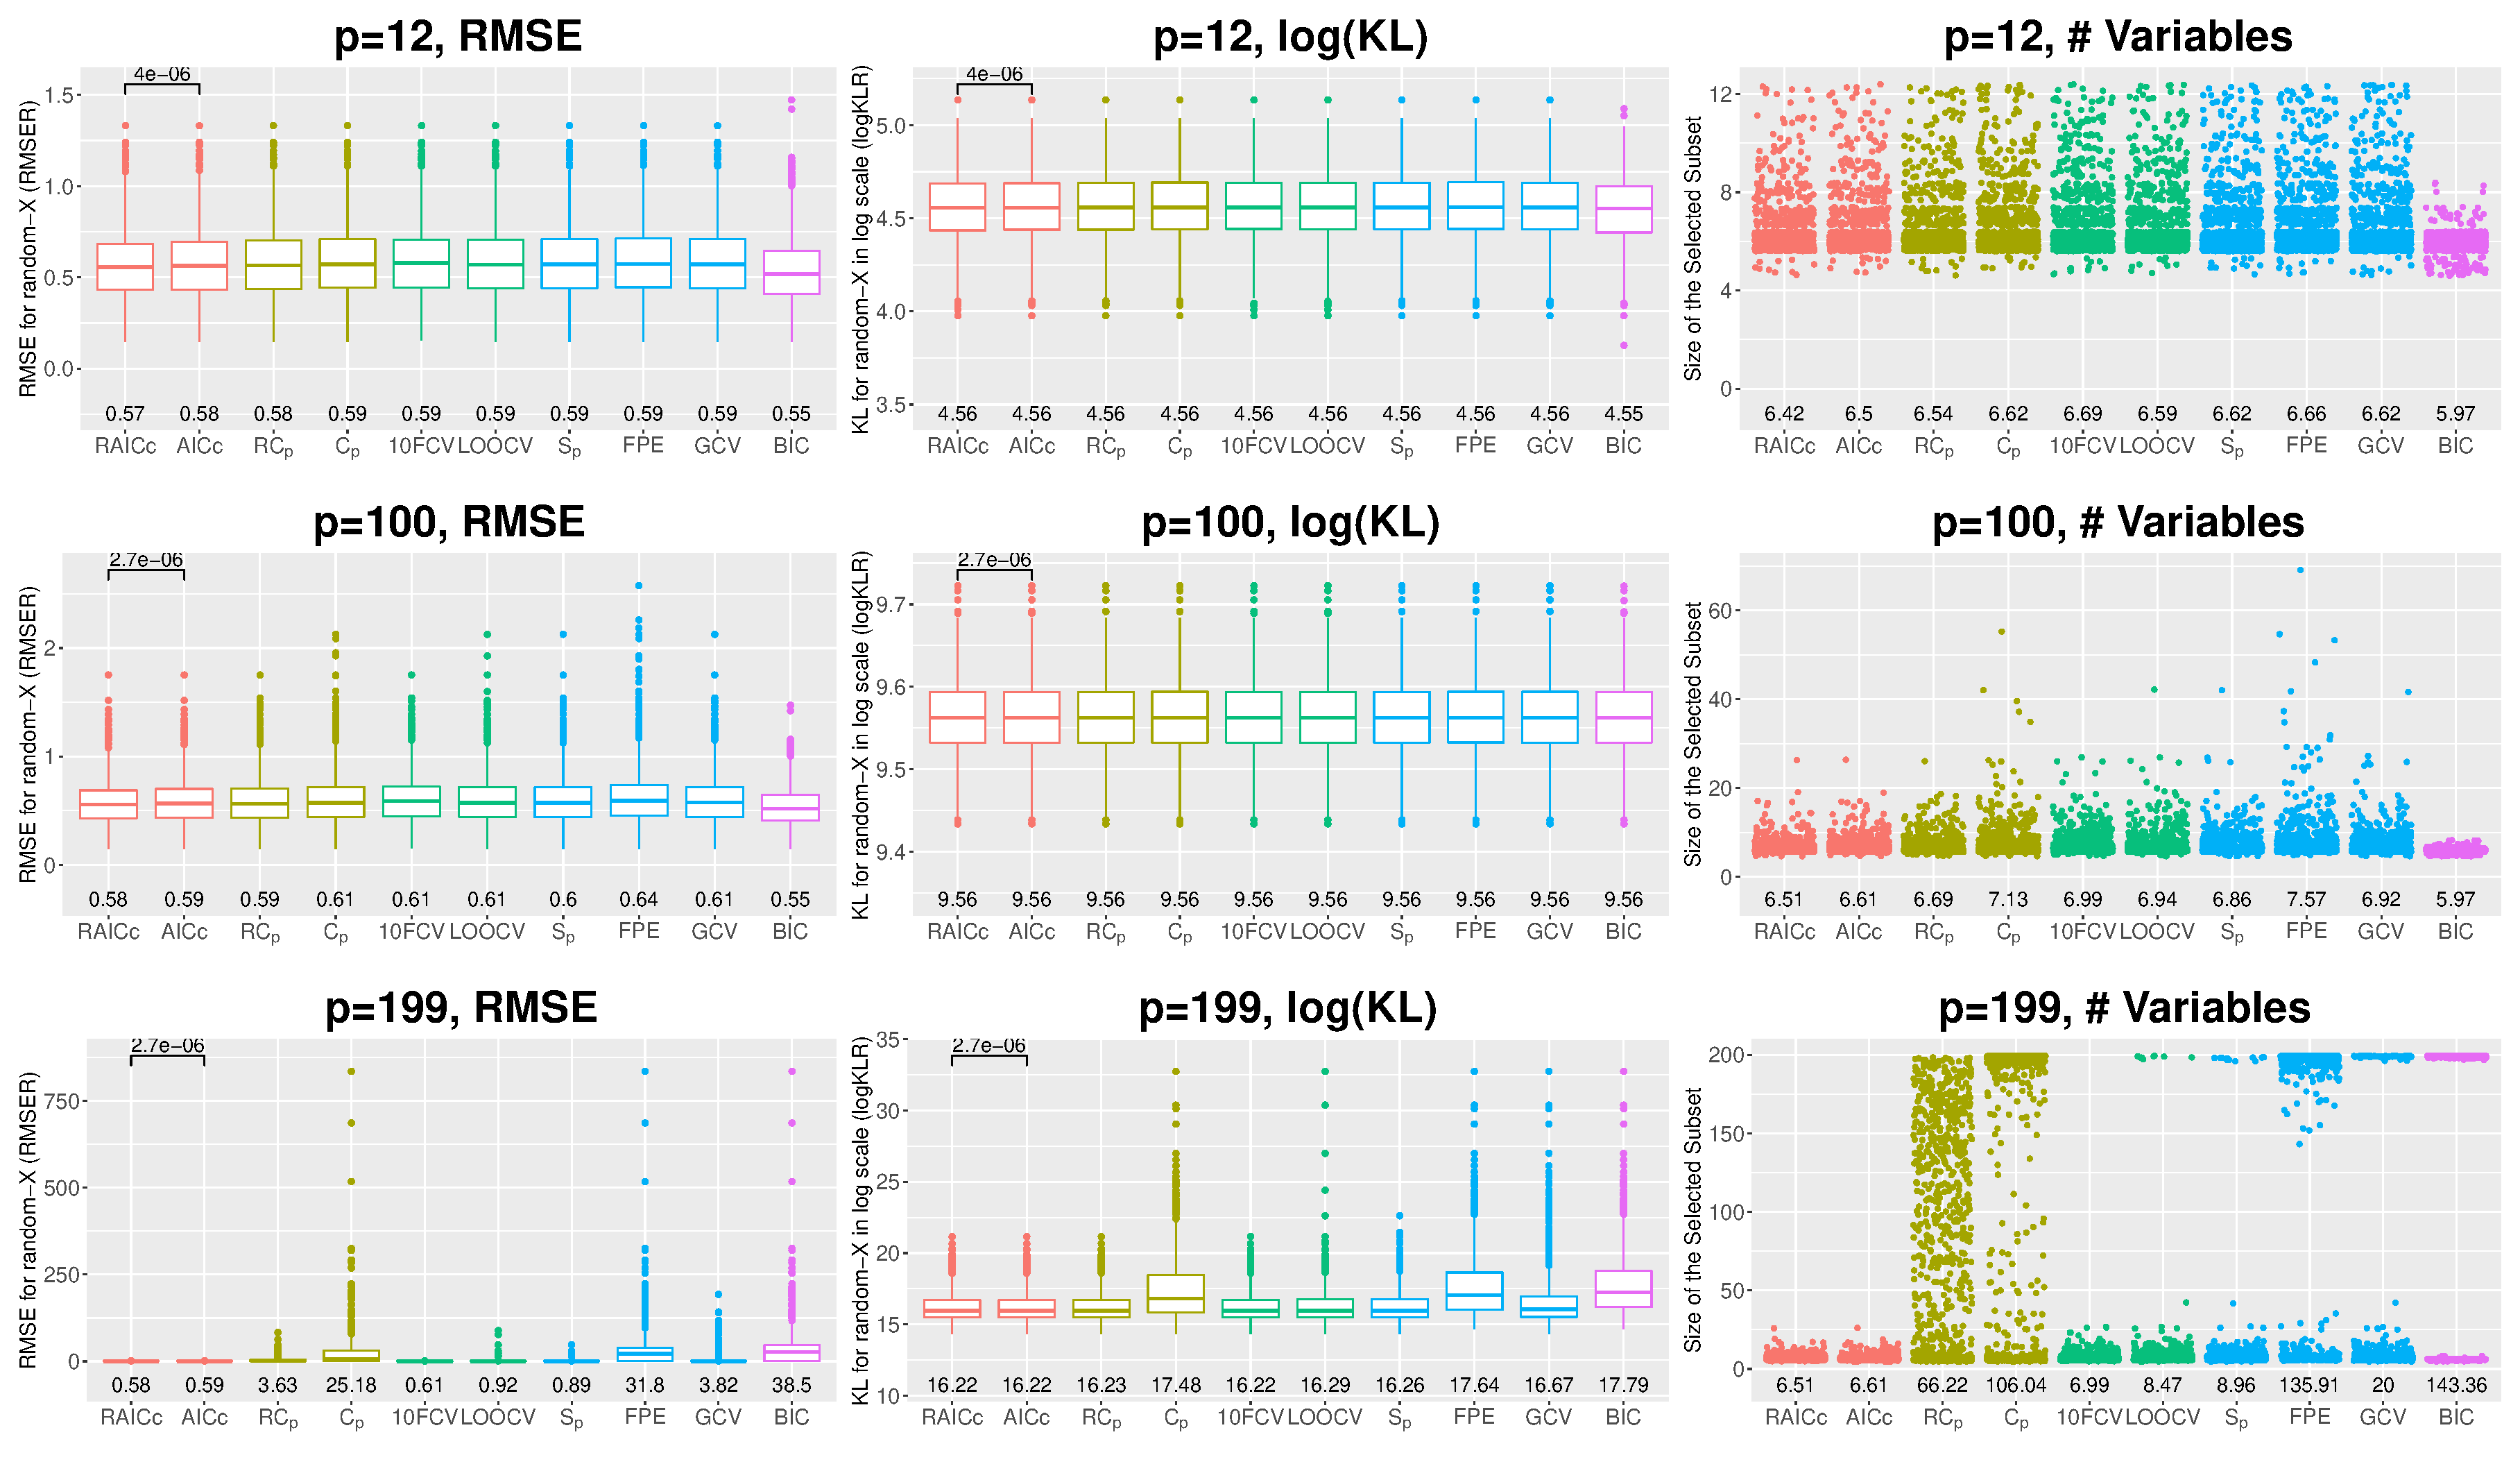
\includegraphics[width=\textwidth]{figures/supplement/randomx_VS-Ex1_n200_hsnr_rho05.eps}
\caption{VS-Ex1, $n=200$, high signal, $\rho=0.5$, and Random-X.}
\end{figure}
\begin{figure}[!ht]
\centering
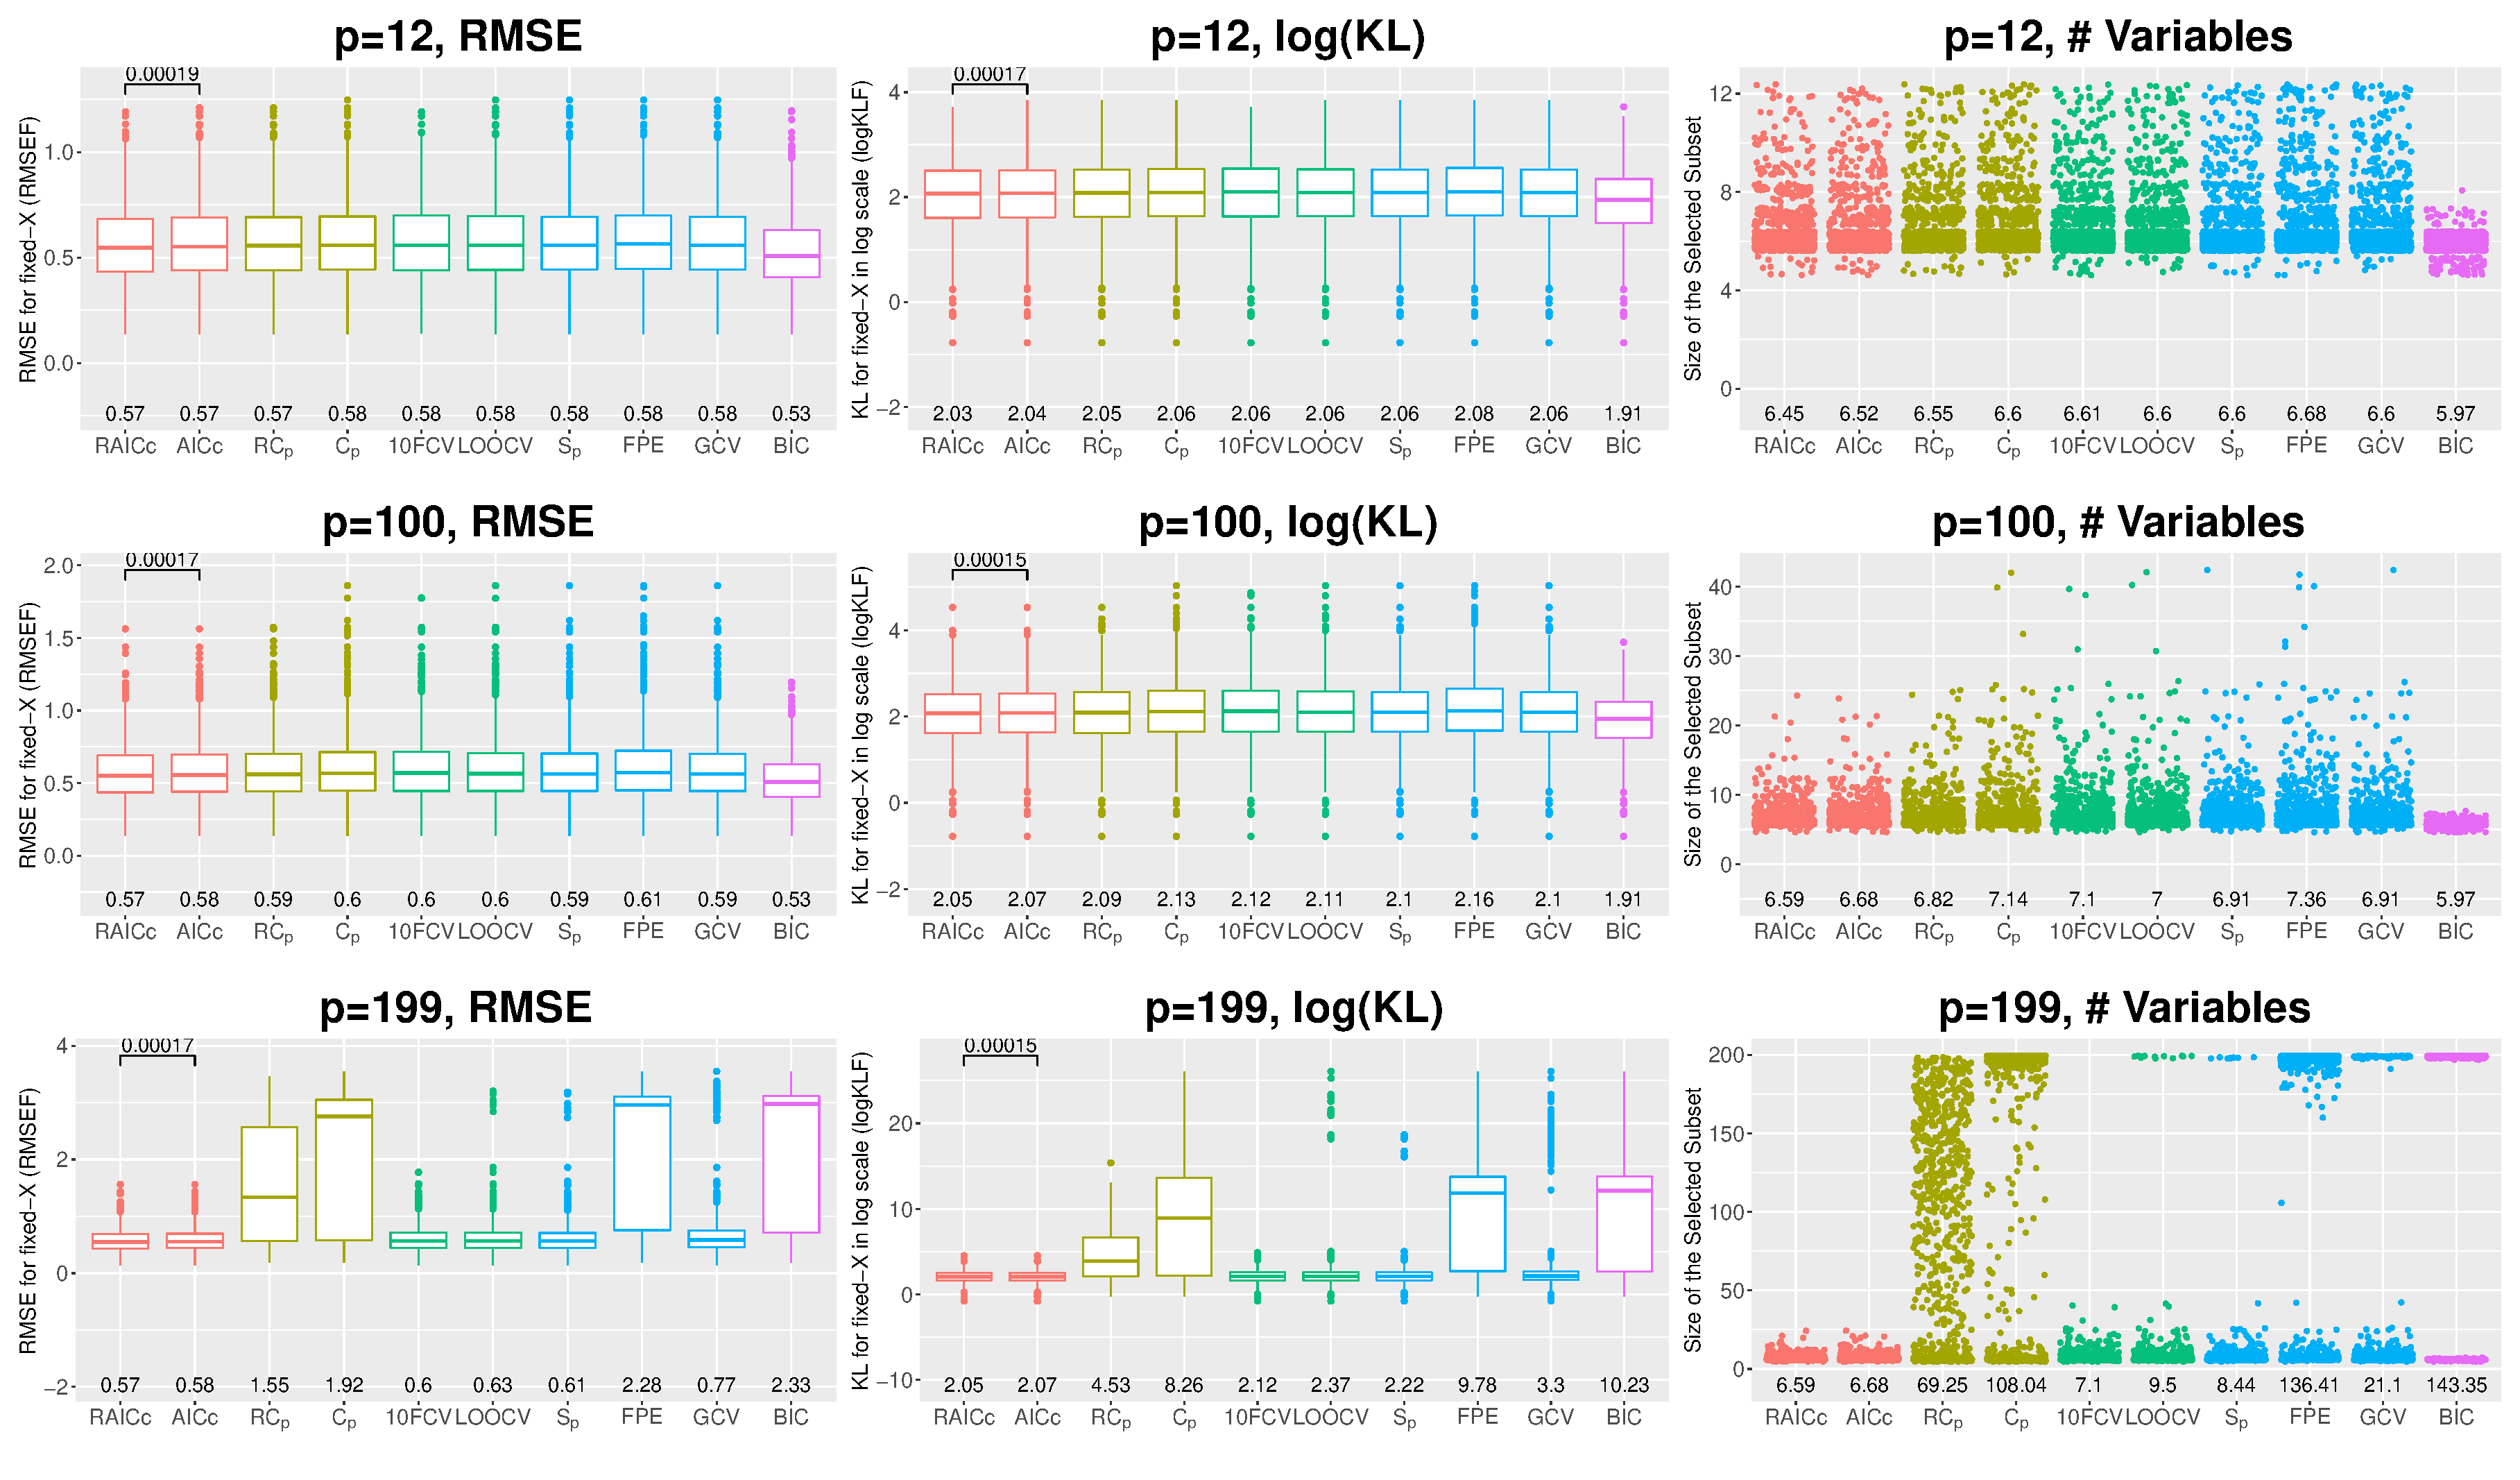
\includegraphics[width=\textwidth]{figures/supplement/fixedx_VS-Ex1_n200_hsnr_rho05.eps}
\caption{VS-Ex1, $n=200$, high signal, $\rho=0.5$, and Fixed-X.}
\end{figure}
\clearpage
\begin{figure}[!ht]
\centering
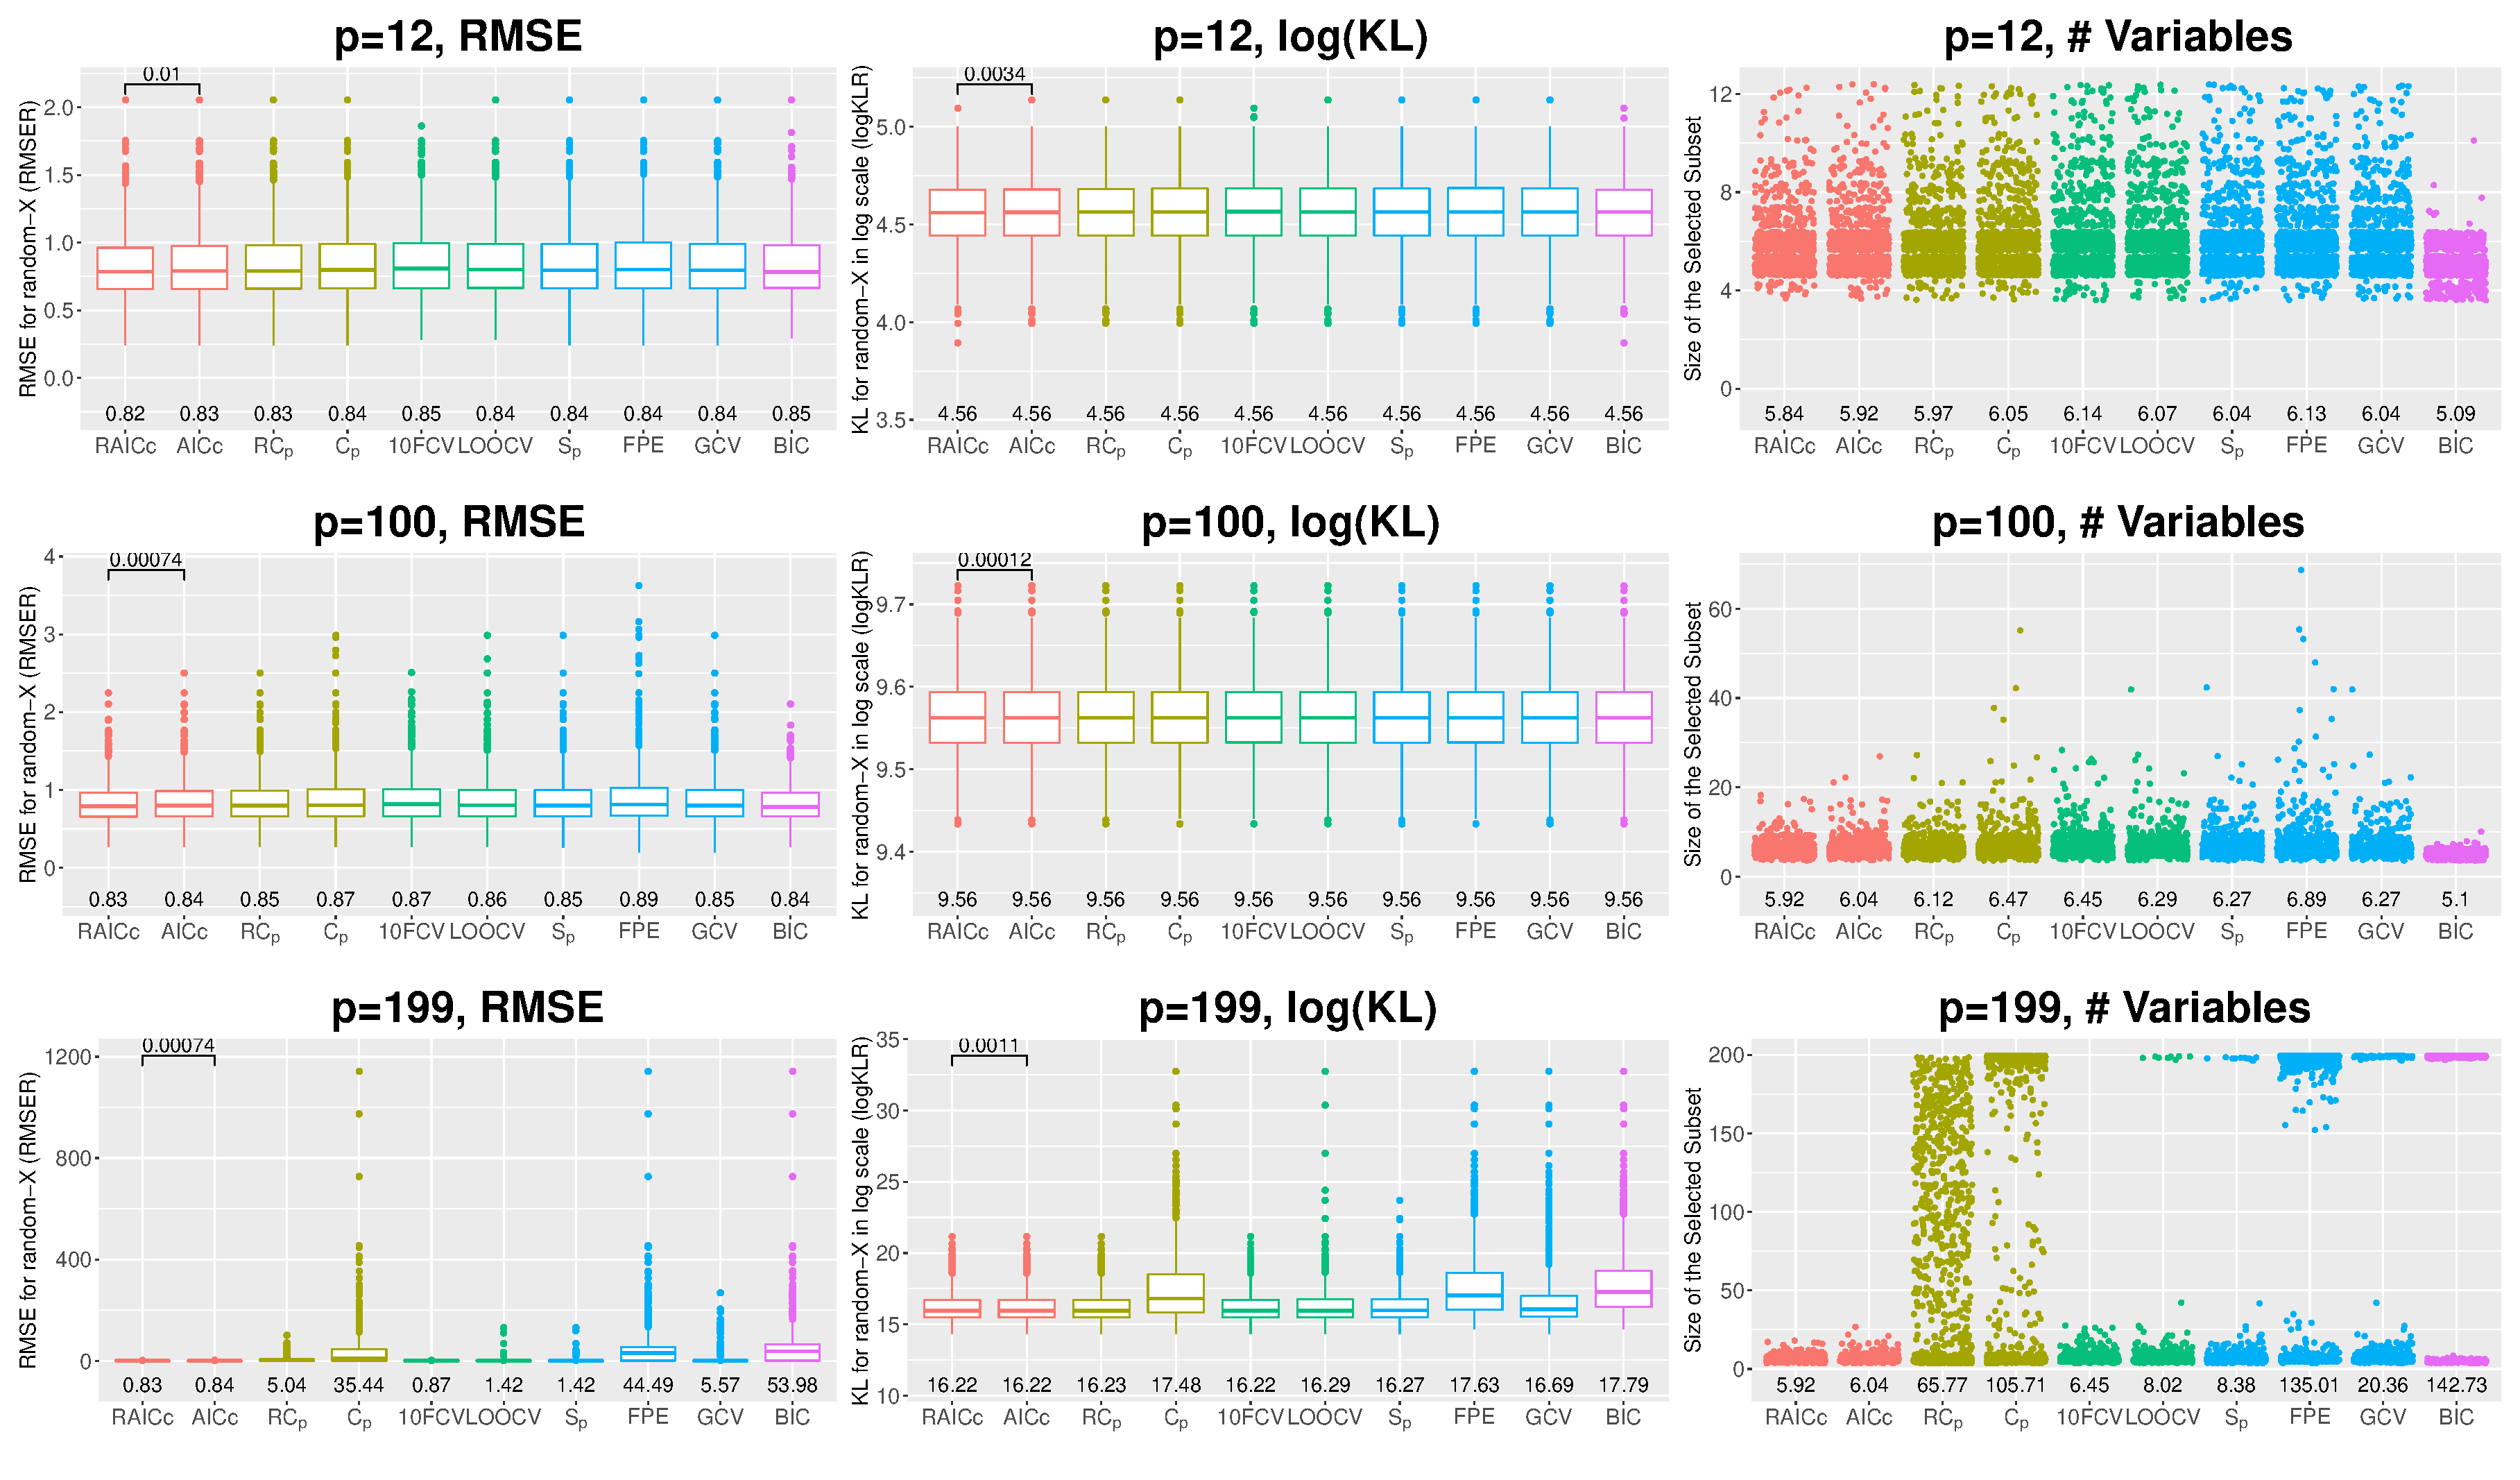
\includegraphics[width=\textwidth]{figures/supplement/randomx_VS-Ex1_n200_hsnr_rho09.eps}
\caption{VS-Ex1, $n=200$, high signal, $\rho=0.9$, and Random-X.}
\end{figure}
\begin{figure}[!ht]
\centering
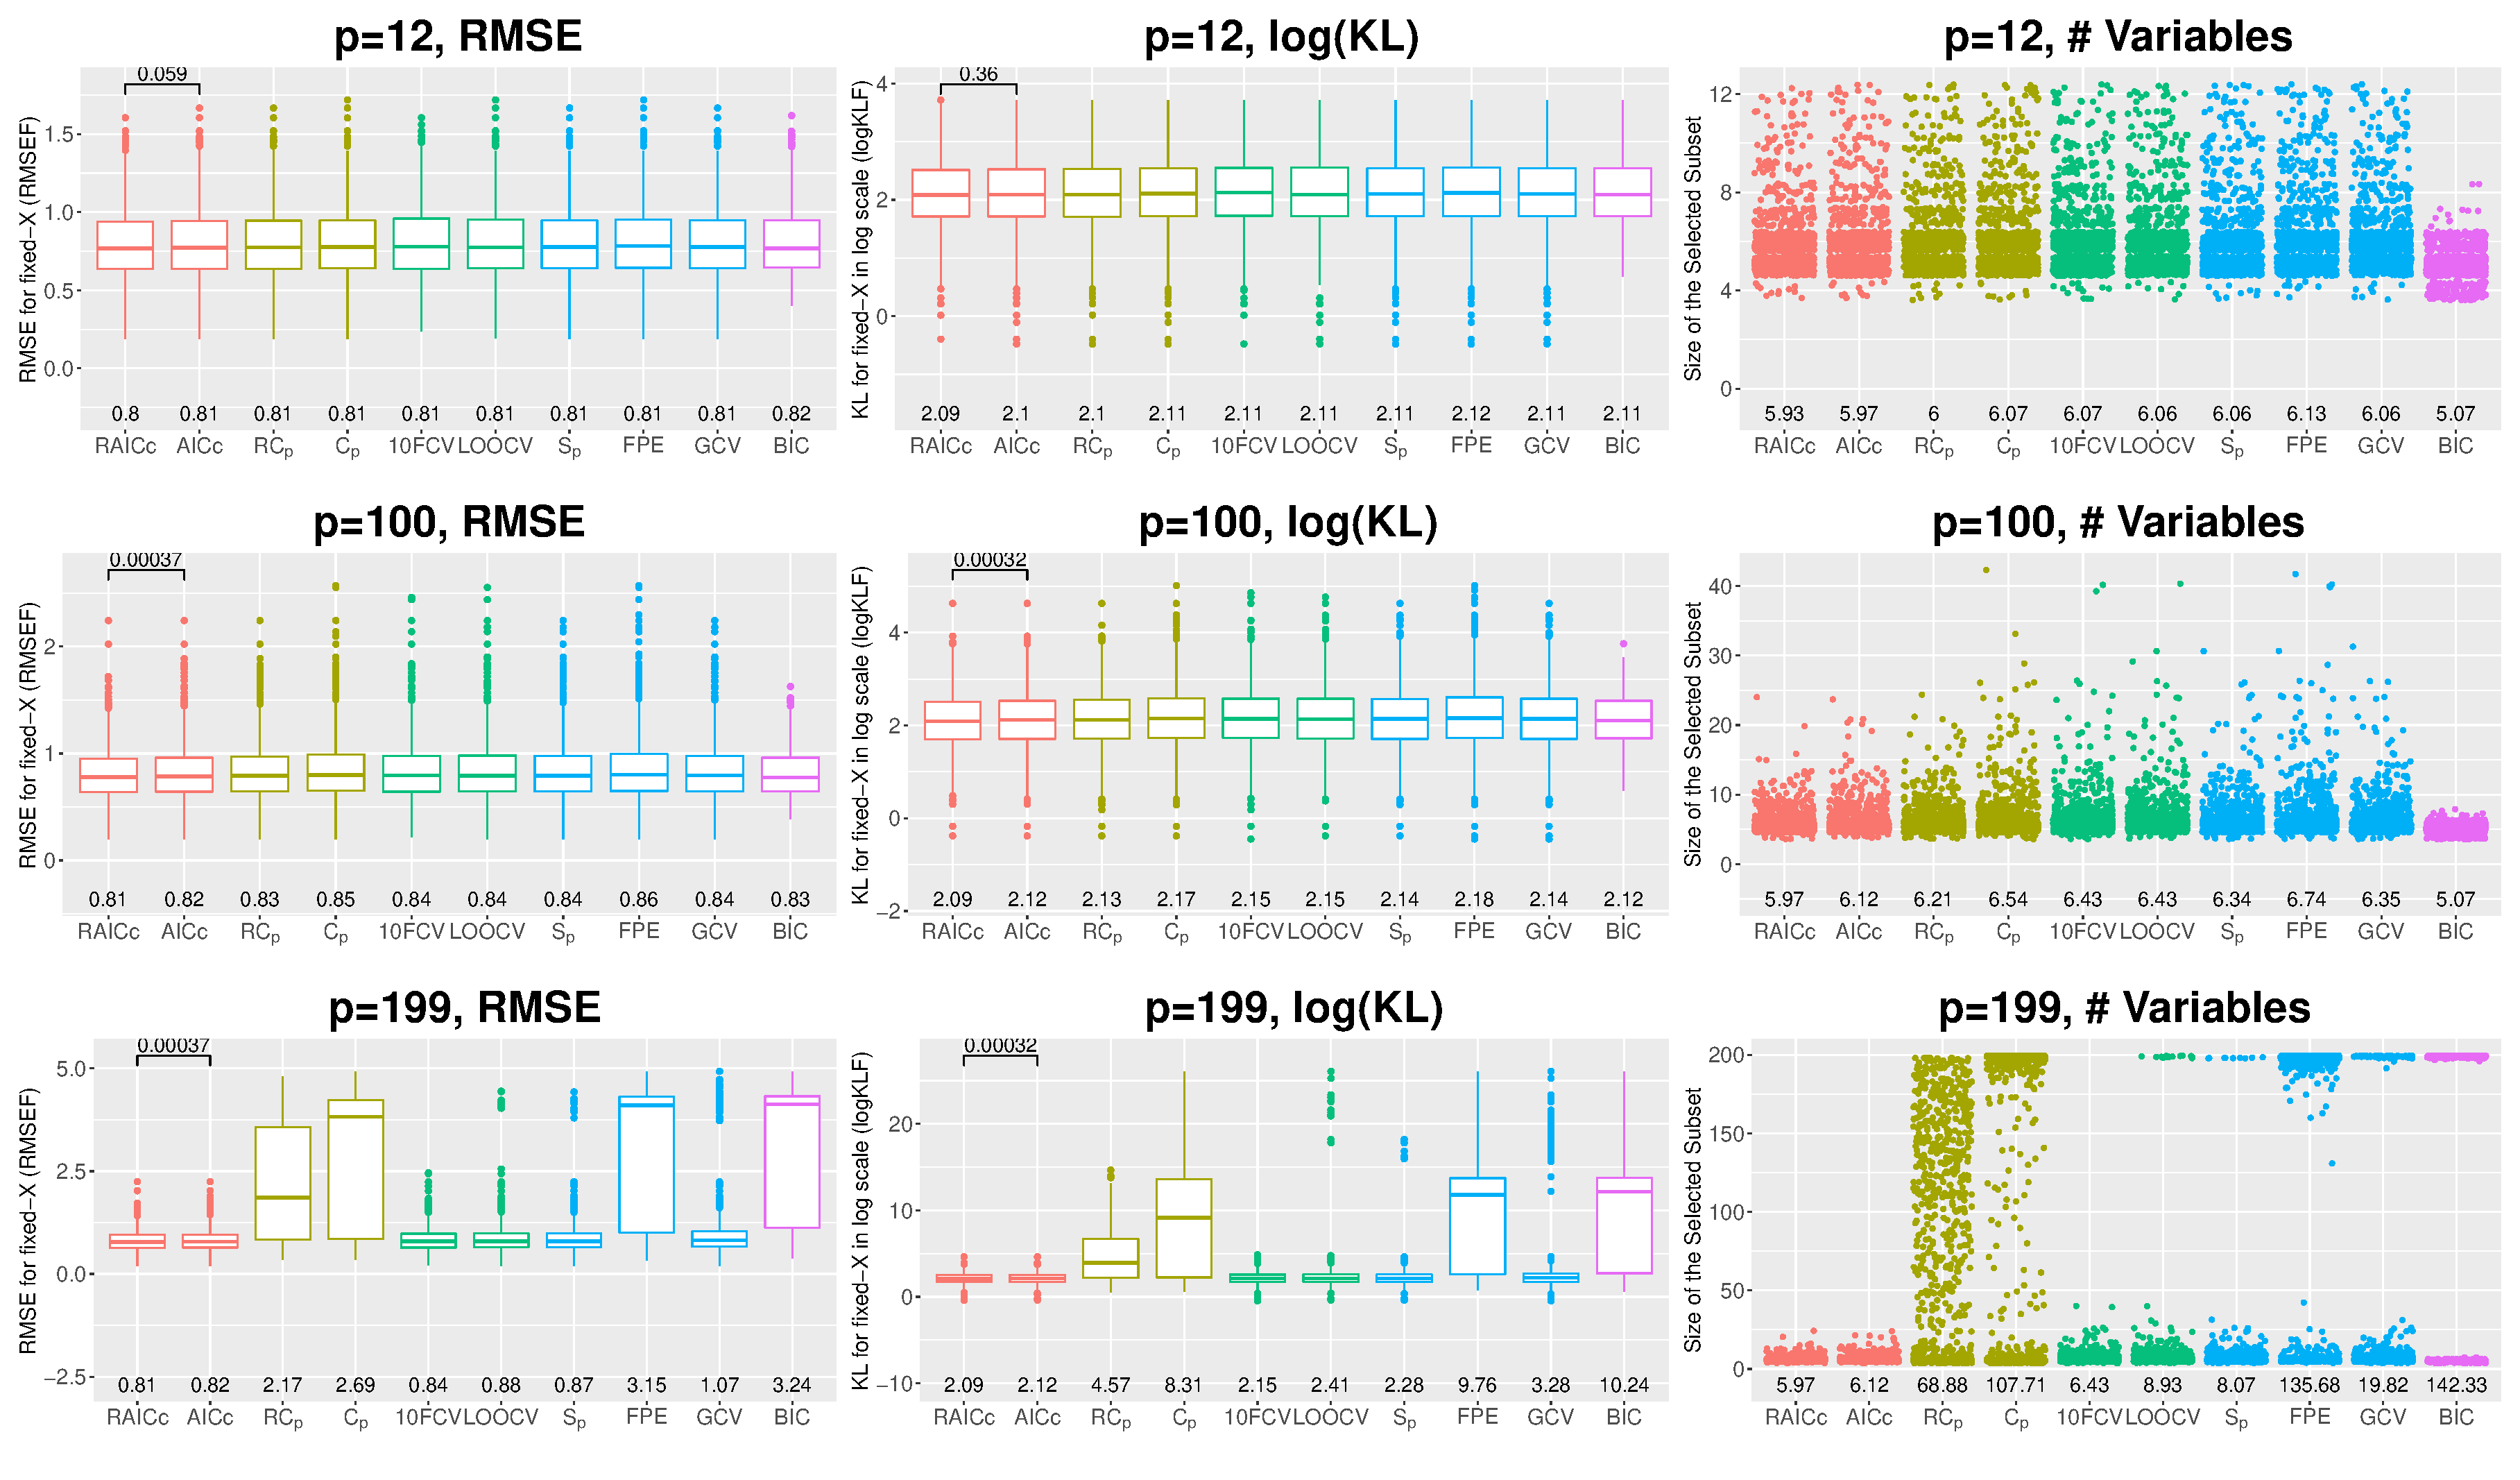
\includegraphics[width=\textwidth]{figures/supplement/fixedx_VS-Ex1_n200_hsnr_rho09.eps}
\caption{VS-Ex1, $n=200$, high signal, $\rho=0.9$, and Fixed-X.}
\end{figure}
\clearpage
\begin{figure}[!ht]
\centering
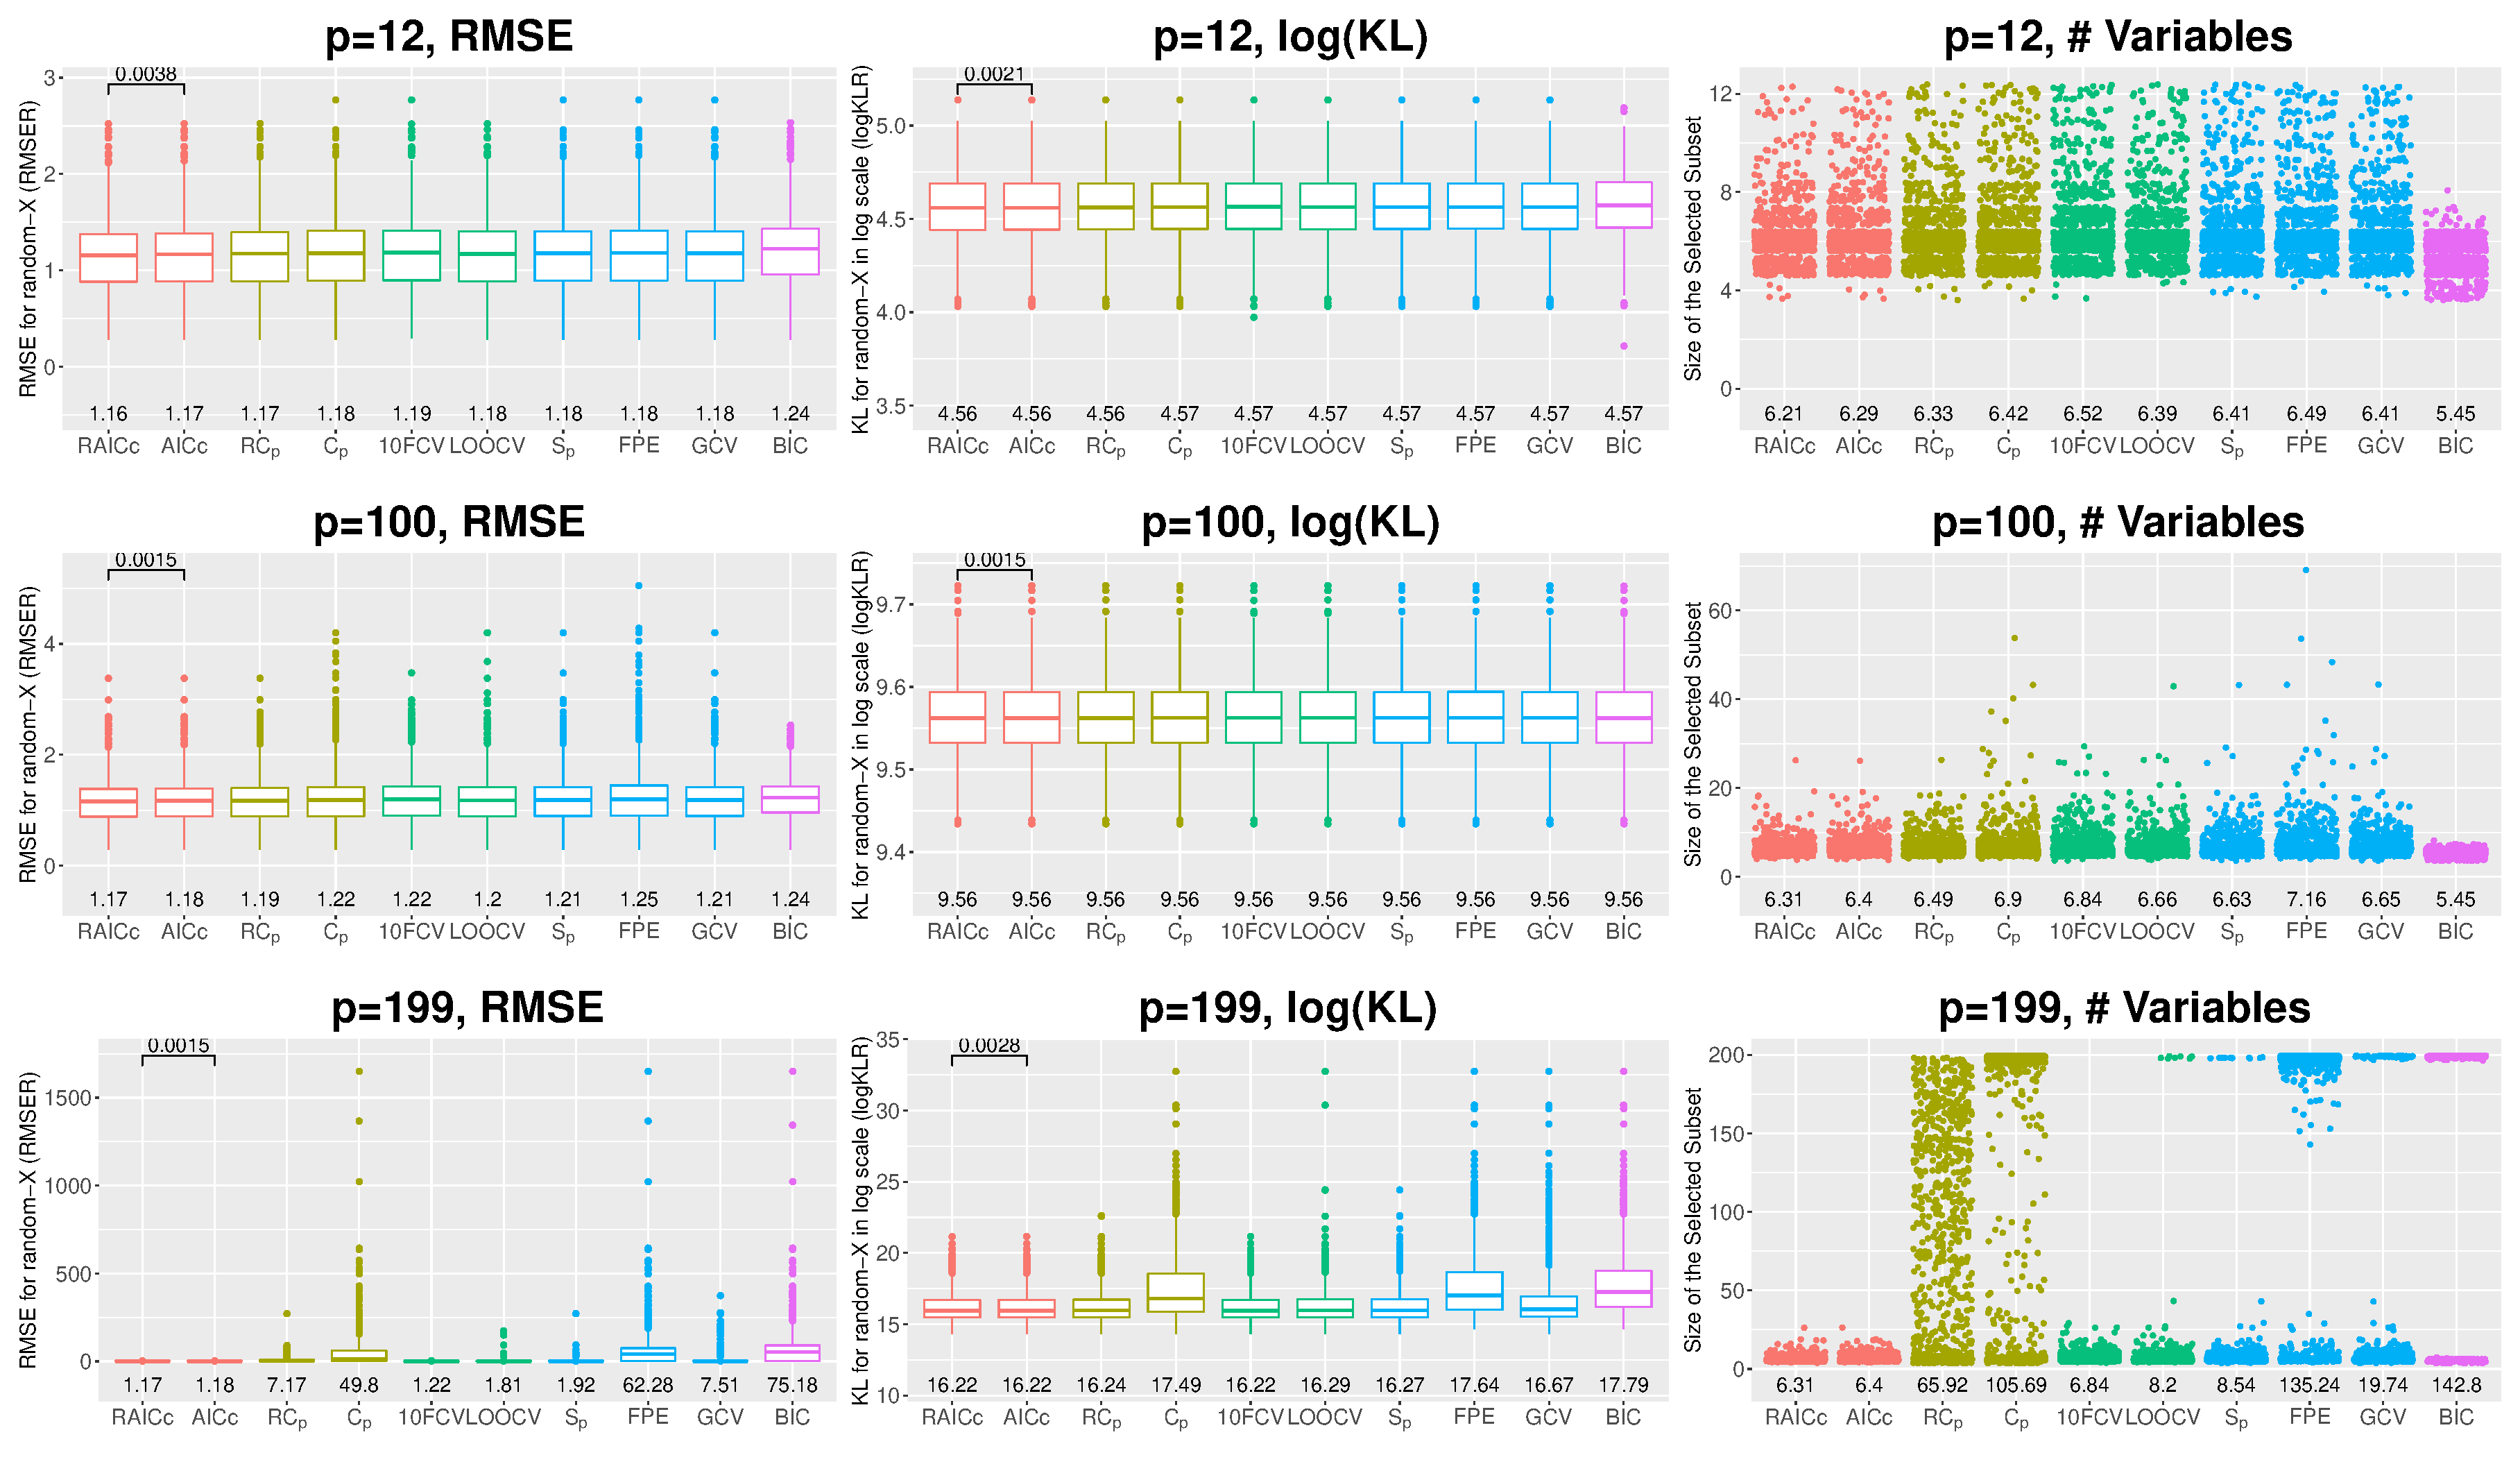
\includegraphics[width=\textwidth]{figures/supplement/randomx_VS-Ex1_n200_msnr_rho0.eps}
\caption{VS-Ex1, $n=200$, medium signal, $\rho=0$, and Random-X.}
\end{figure}
\begin{figure}[!ht]
\centering
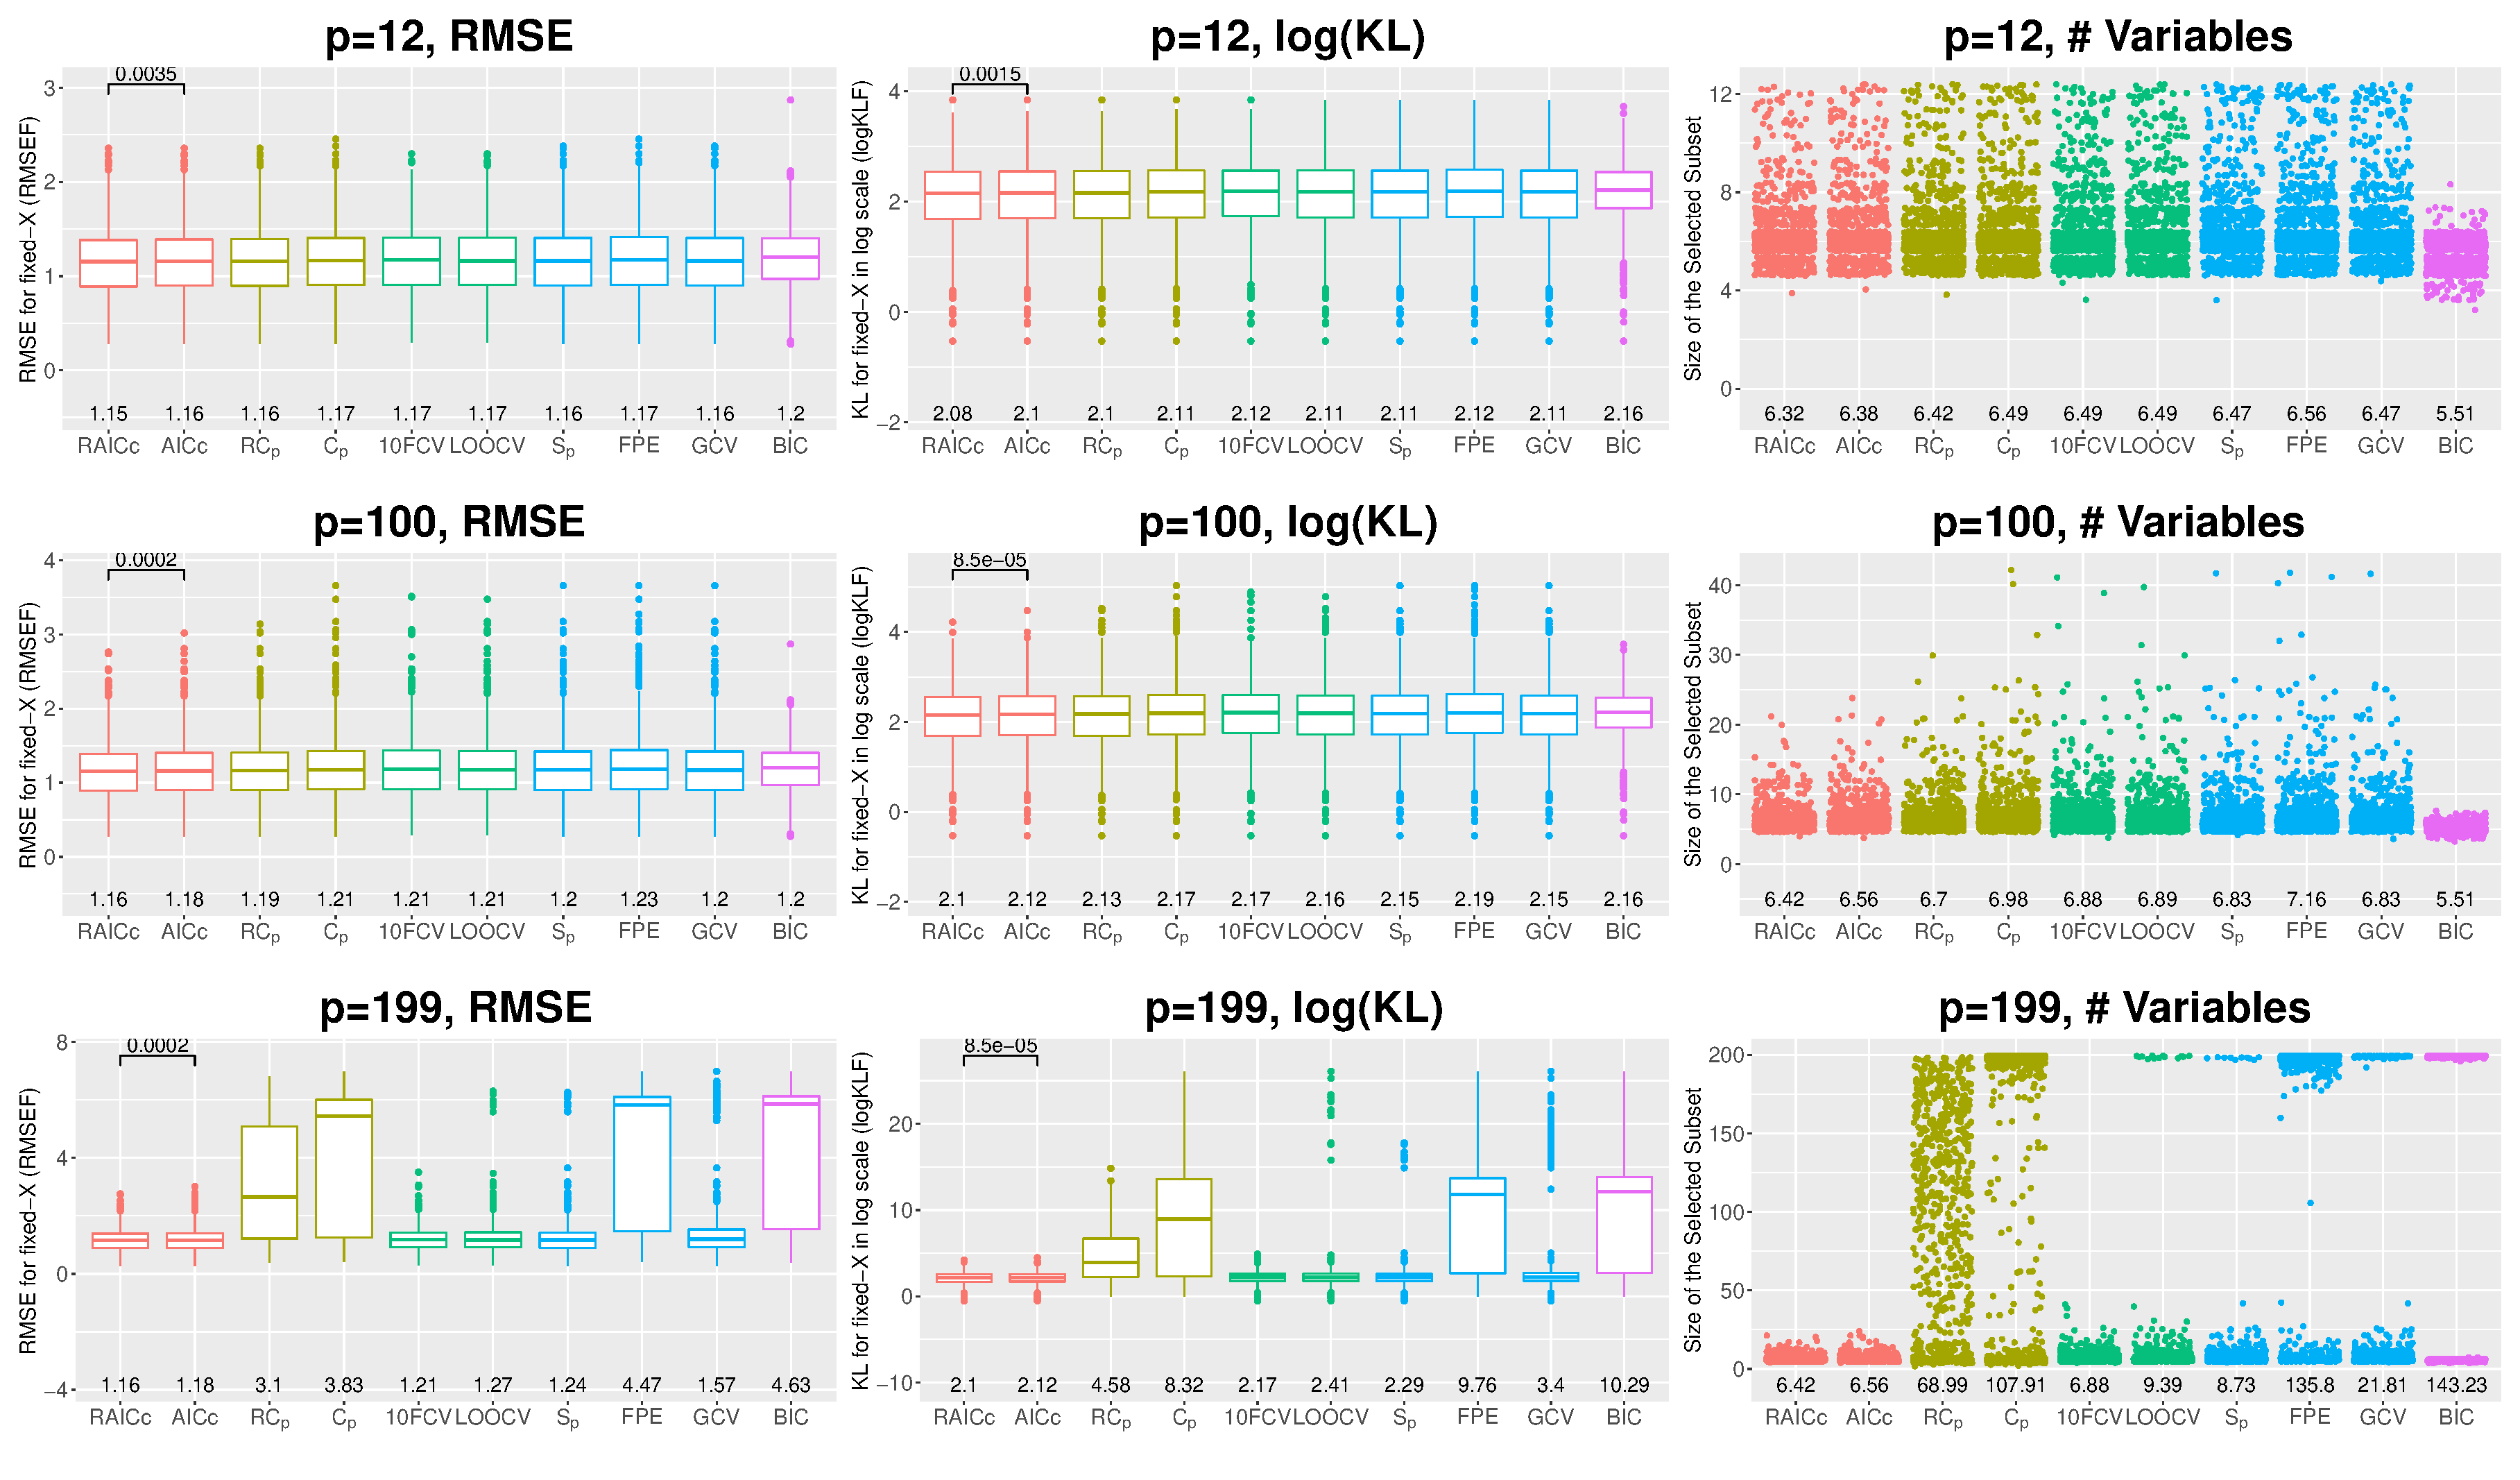
\includegraphics[width=\textwidth]{figures/supplement/fixedx_VS-Ex1_n200_msnr_rho0.eps}
\caption{VS-Ex1, $n=200$, medium signal, $\rho=0$, and Fixed-X.}
\end{figure}
\clearpage
\begin{figure}[!ht]
\centering
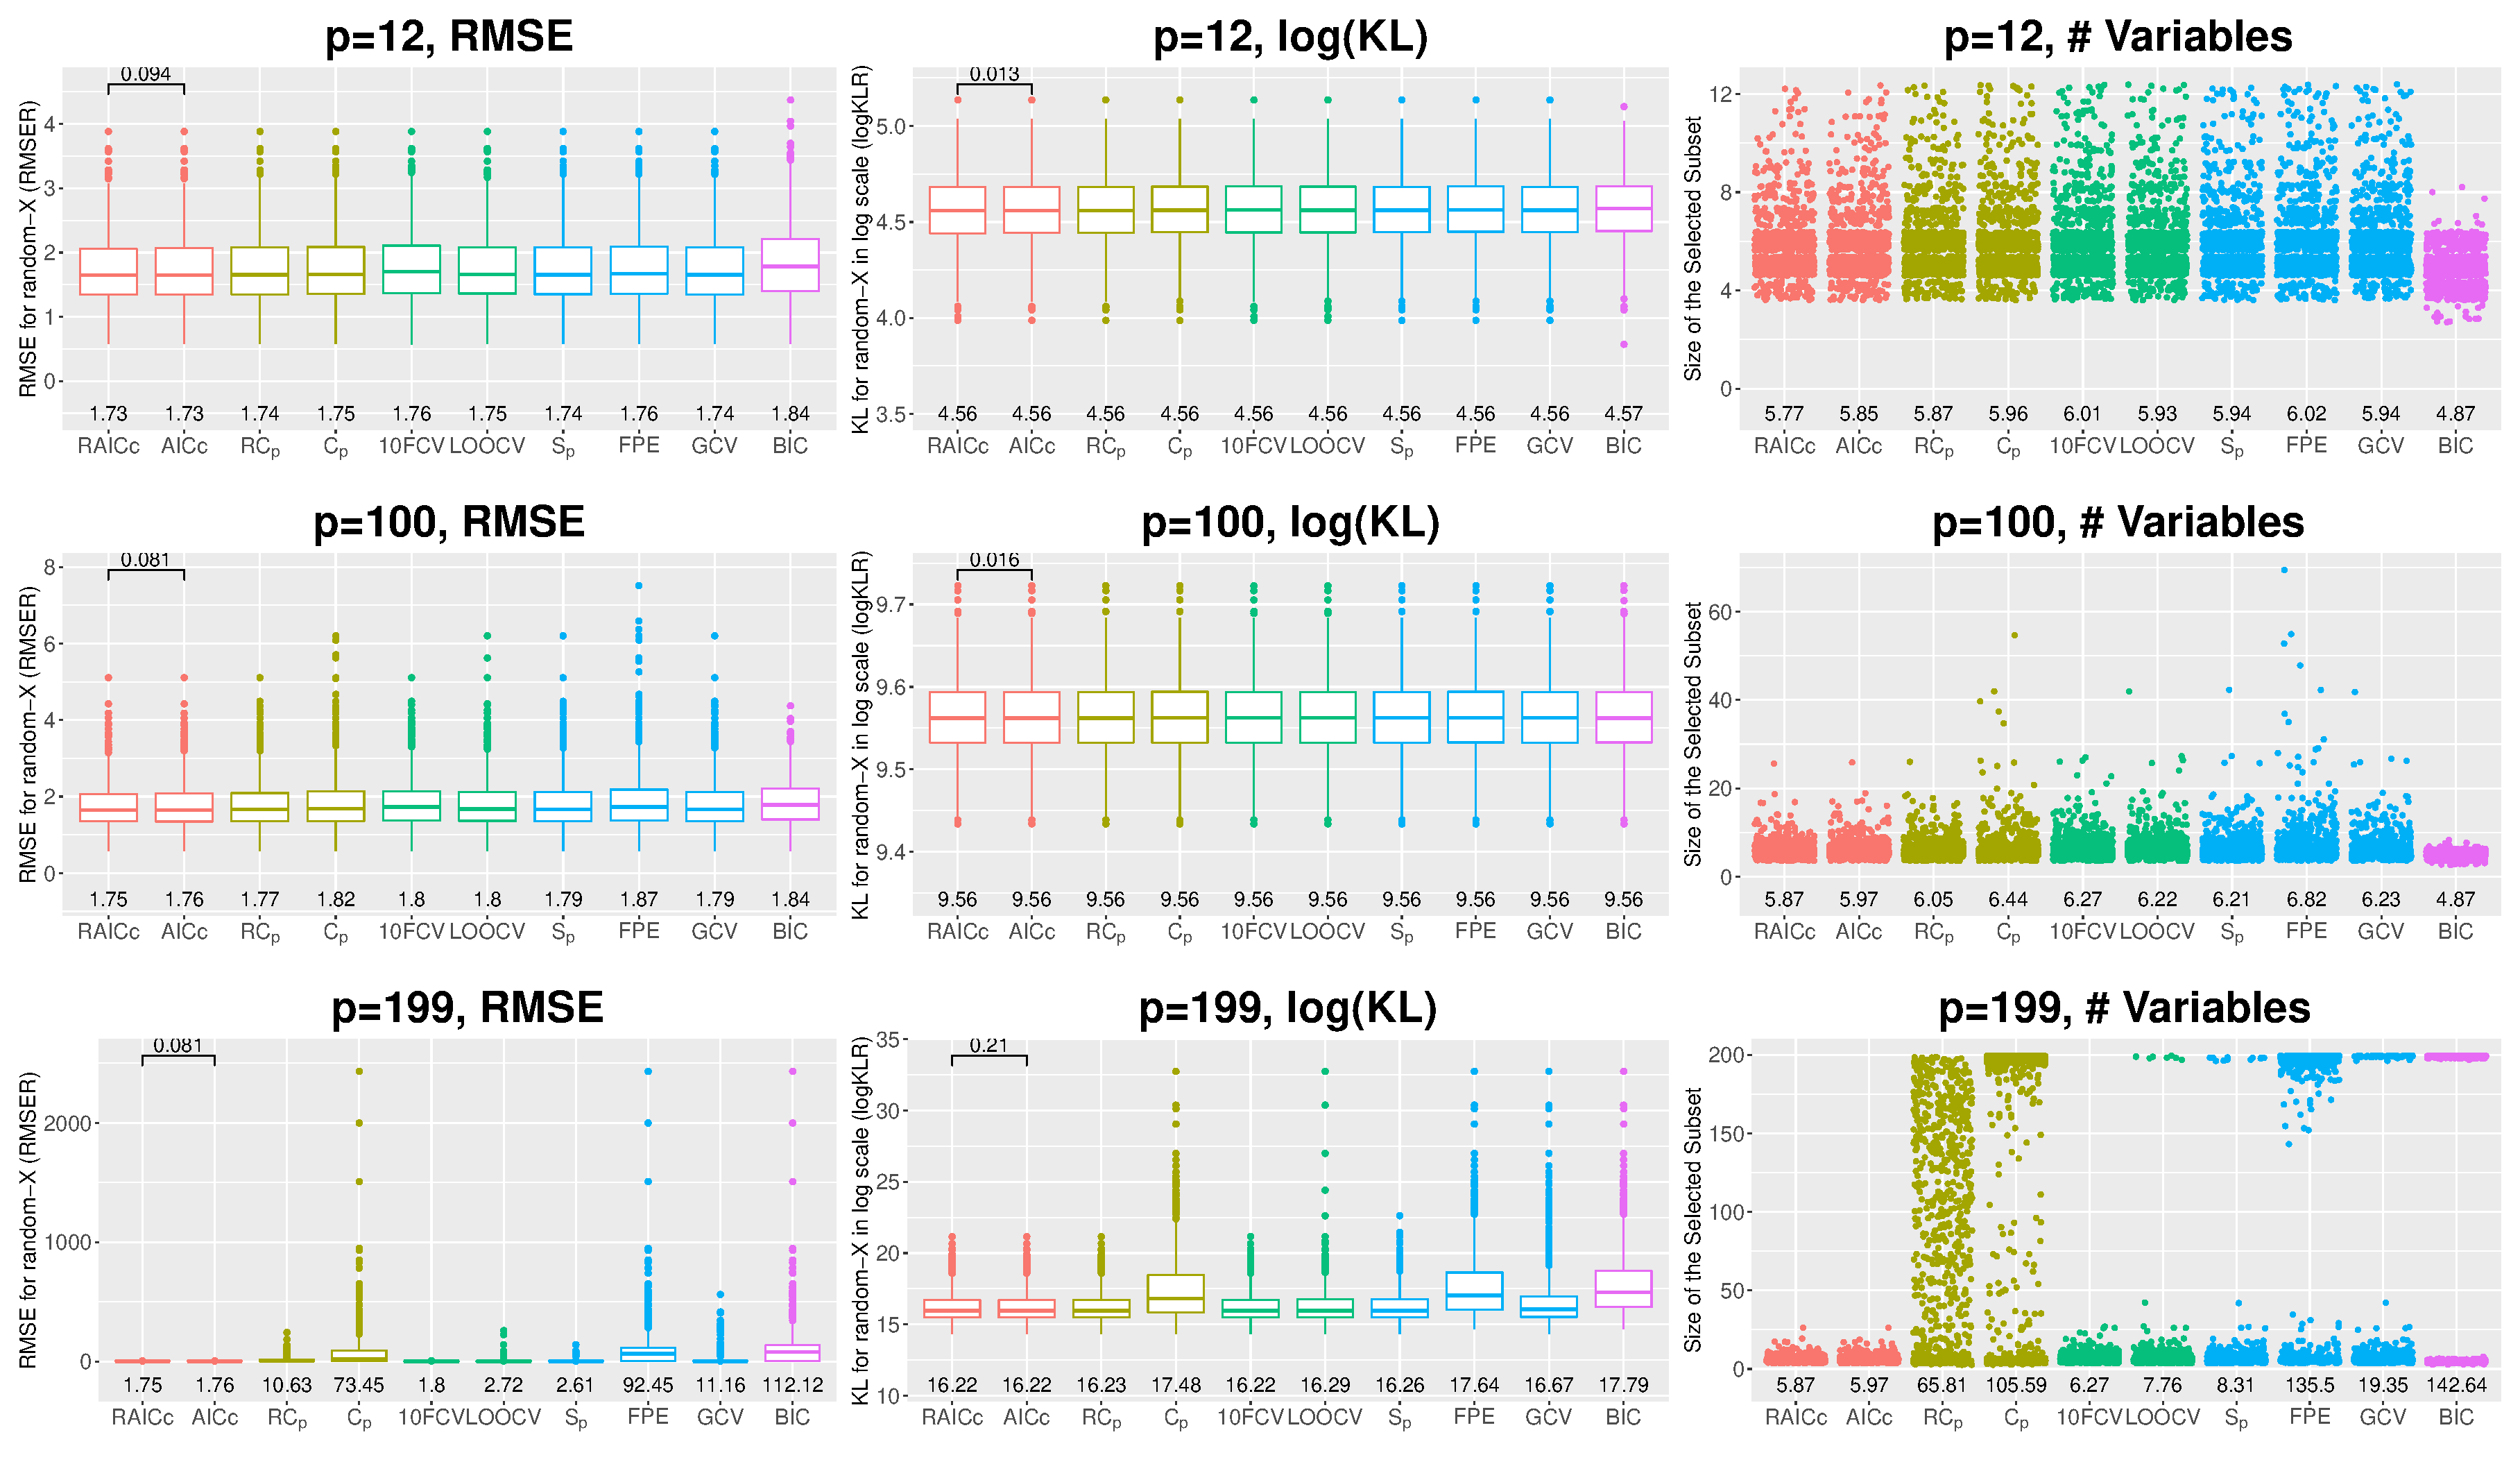
\includegraphics[width=\textwidth]{figures/supplement/randomx_VS-Ex1_n200_msnr_rho05.eps}
\caption{VS-Ex1, $n=200$, medium signal, $\rho=0.5$, and Random-X.}
\end{figure}
\begin{figure}[!ht]
\centering
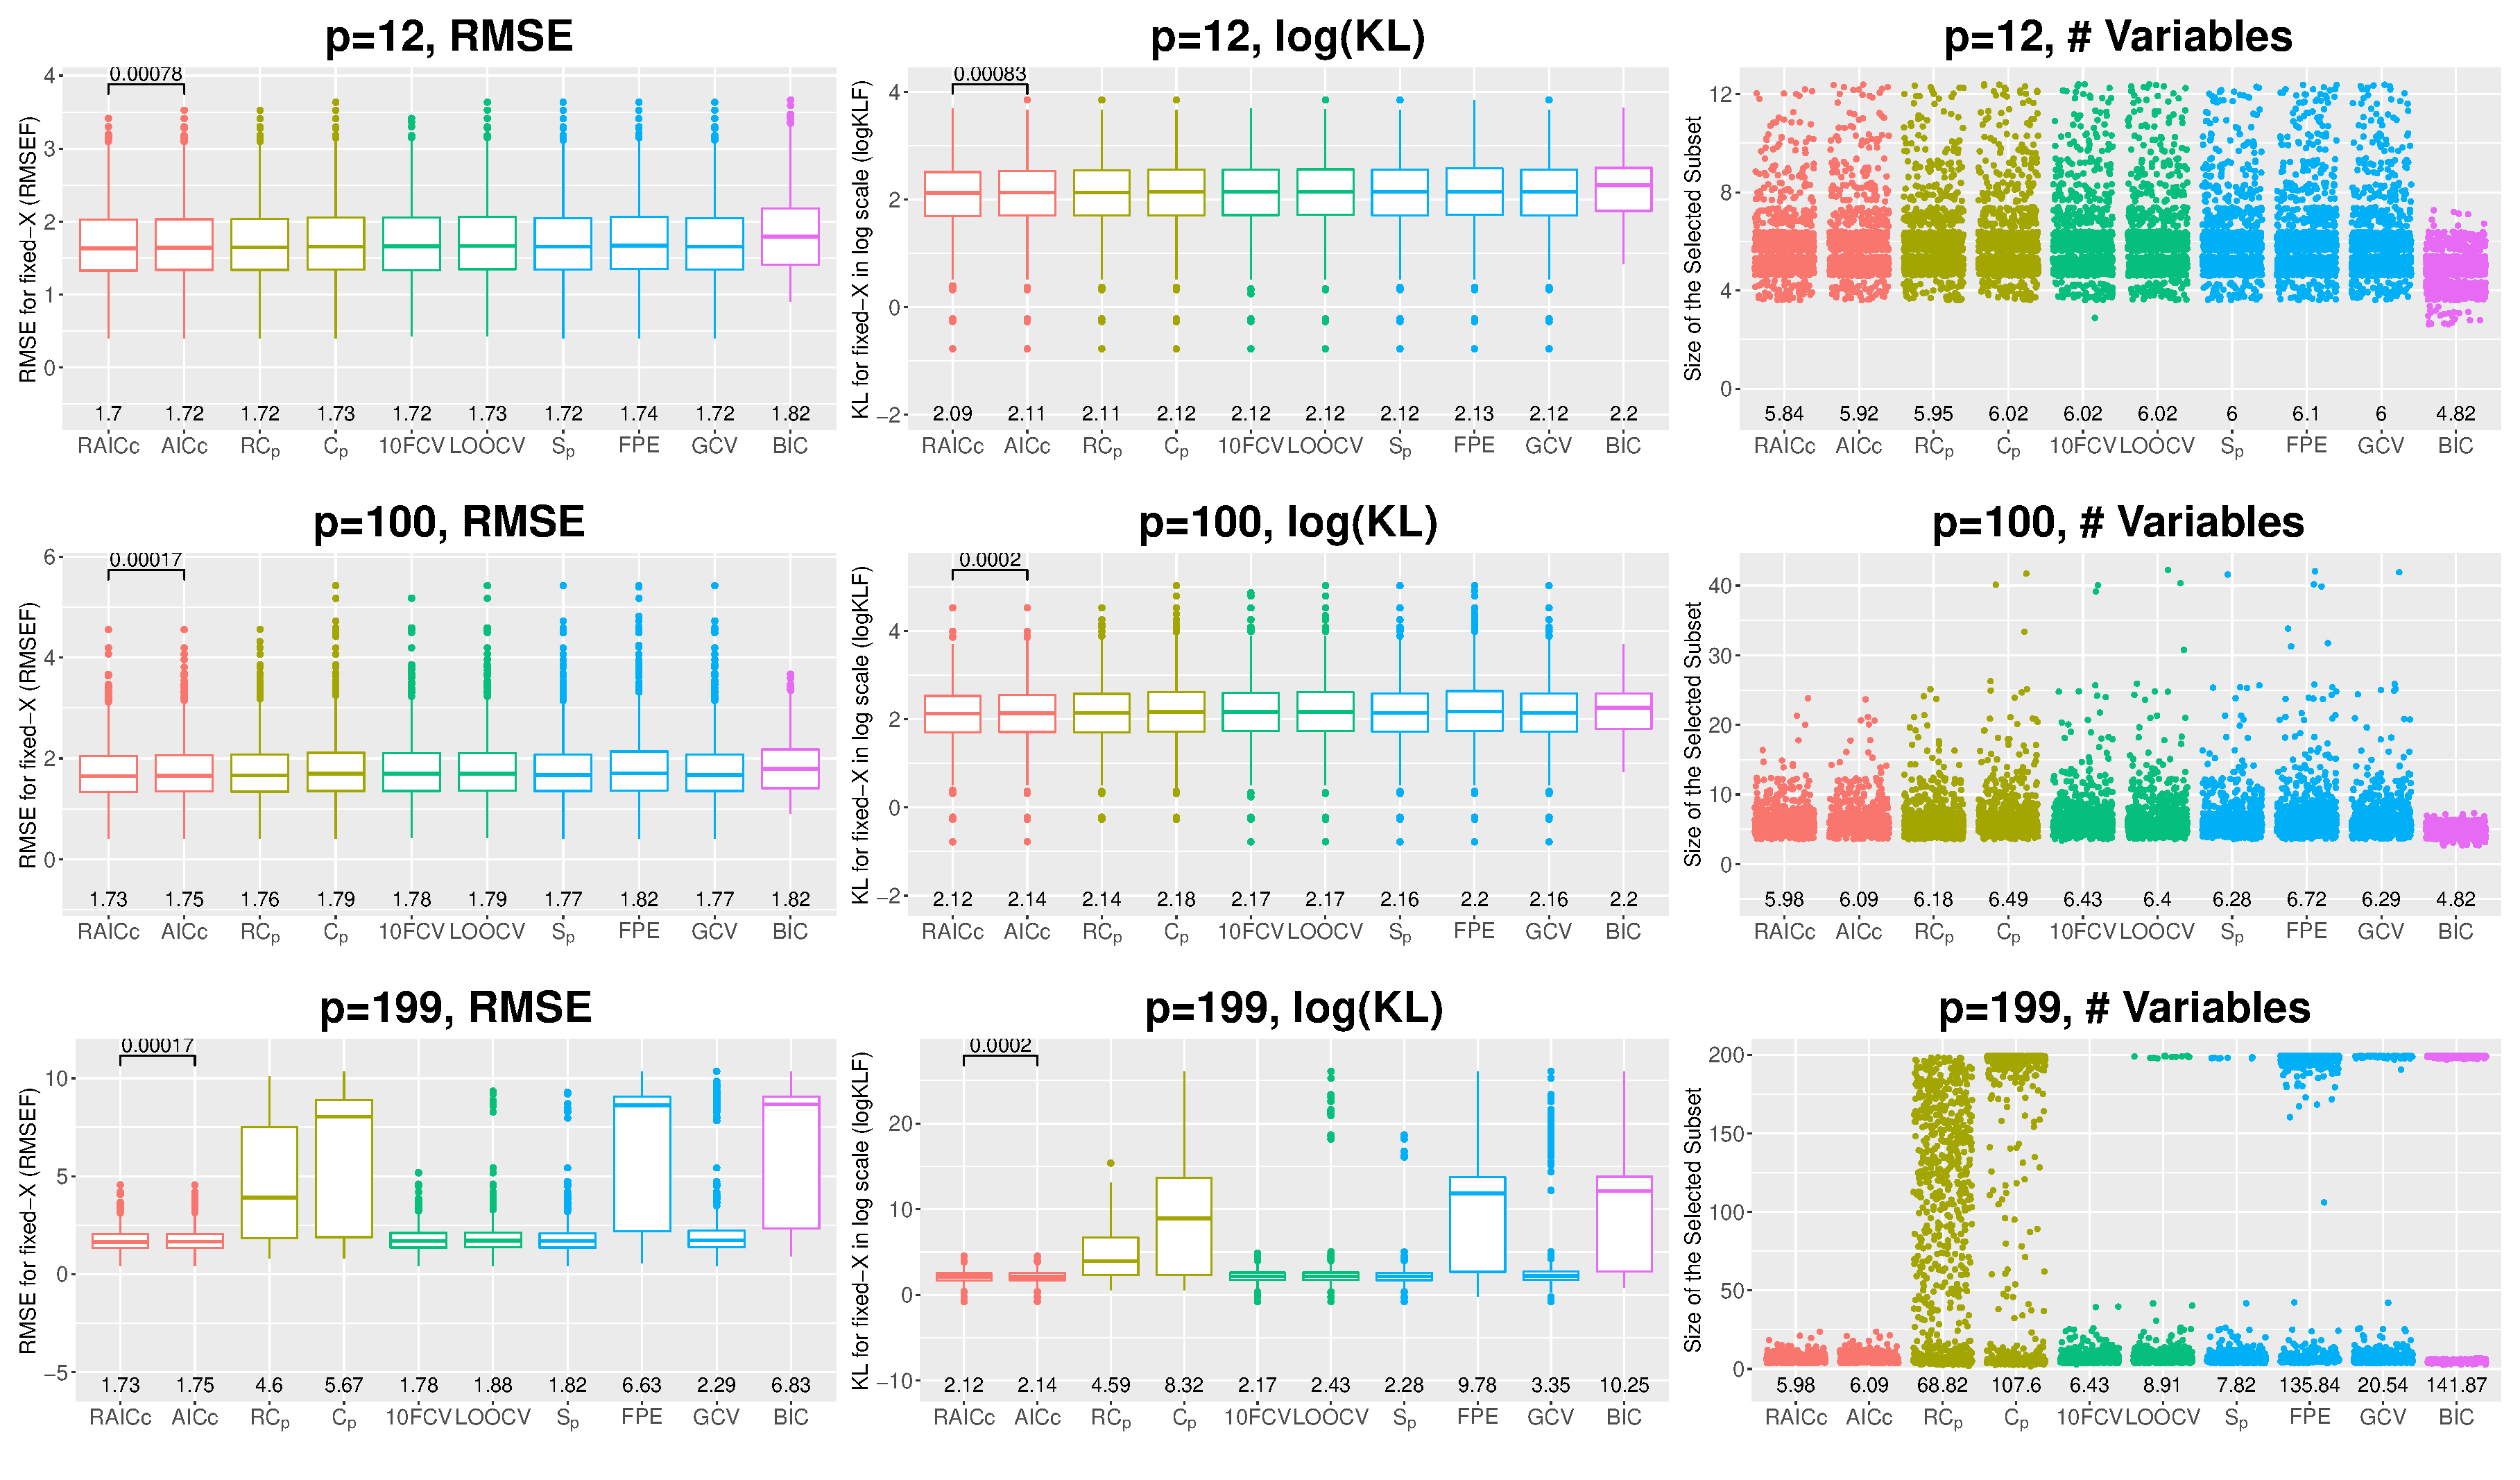
\includegraphics[width=\textwidth]{figures/supplement/fixedx_VS-Ex1_n200_msnr_rho05.eps}
\caption{VS-Ex1, $n=200$, medium signal, $\rho=0.5$, and Fixed-X.}
\end{figure}
\clearpage
\begin{figure}[!ht]
\centering
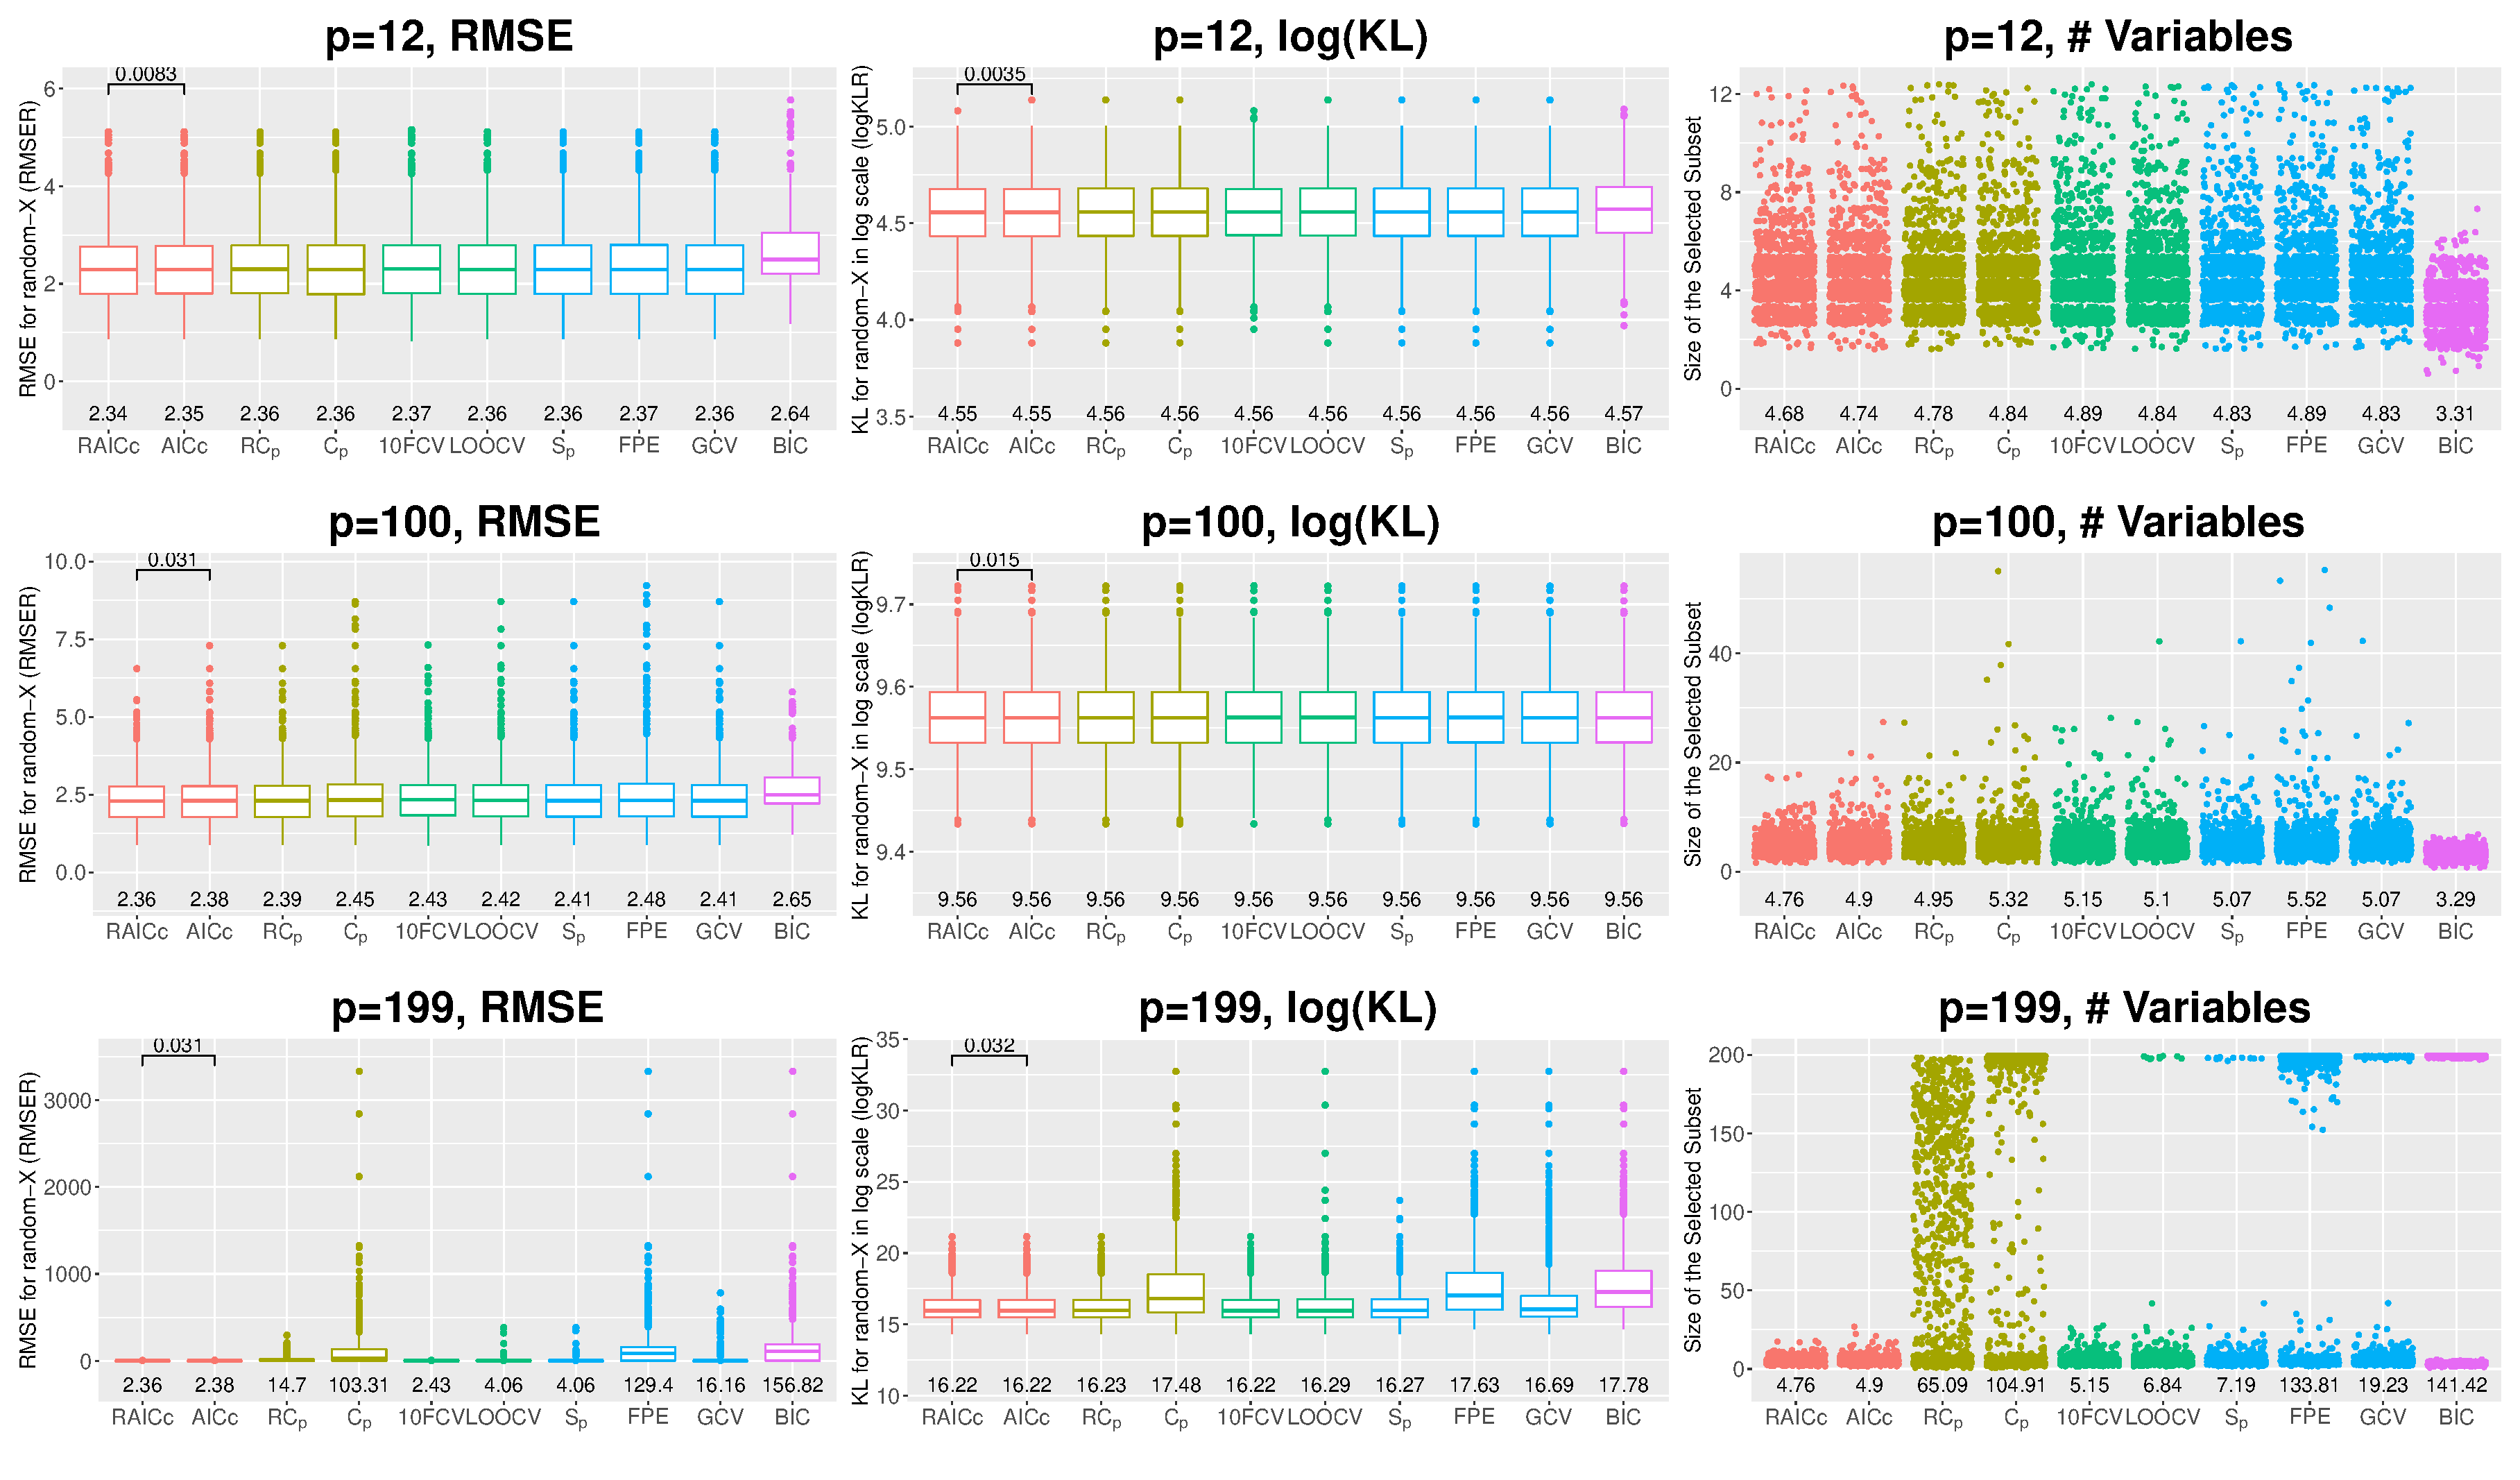
\includegraphics[width=\textwidth]{figures/supplement/randomx_VS-Ex1_n200_msnr_rho09.eps}
\caption{VS-Ex1, $n=200$, medium signal, $\rho=0.9$, and Random-X.}
\end{figure}
\begin{figure}[!ht]
\centering
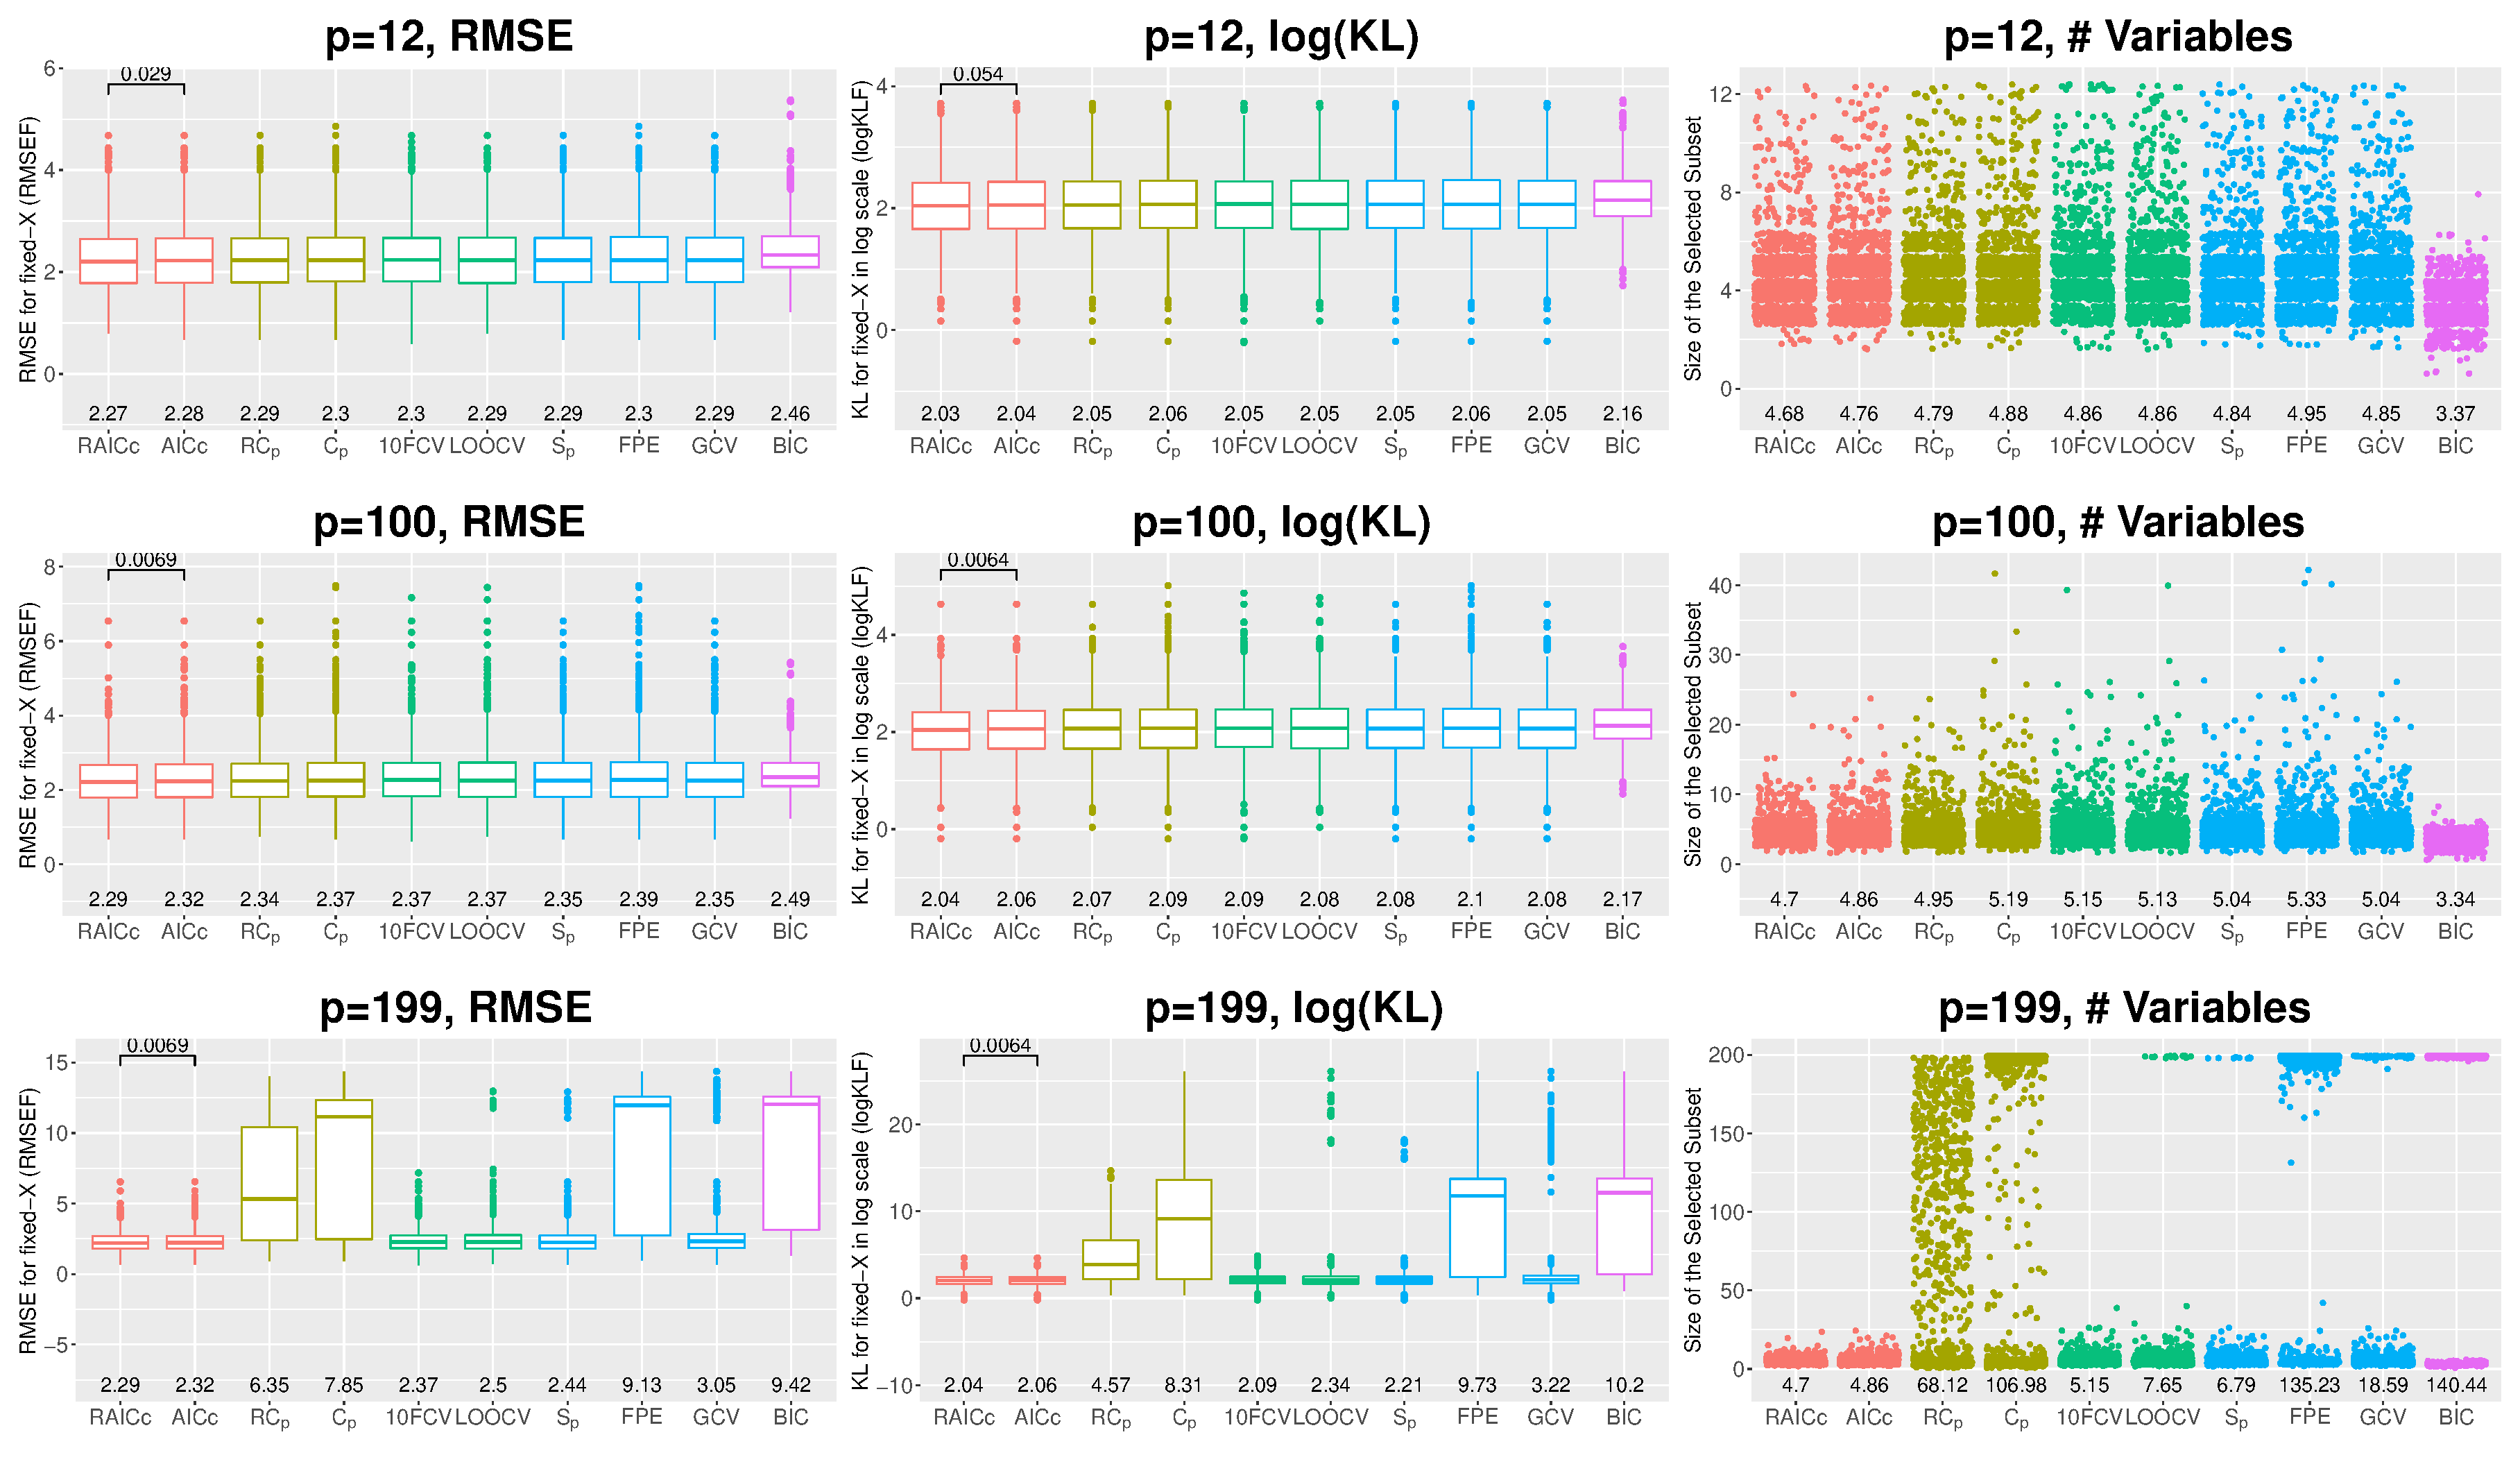
\includegraphics[width=\textwidth]{figures/supplement/fixedx_VS-Ex1_n200_msnr_rho09.eps}
\caption{VS-Ex1, $n=200$, medium signal, $\rho=0.9$, and Fixed-X.}
\end{figure}
\clearpage
\begin{figure}[!ht]
\centering
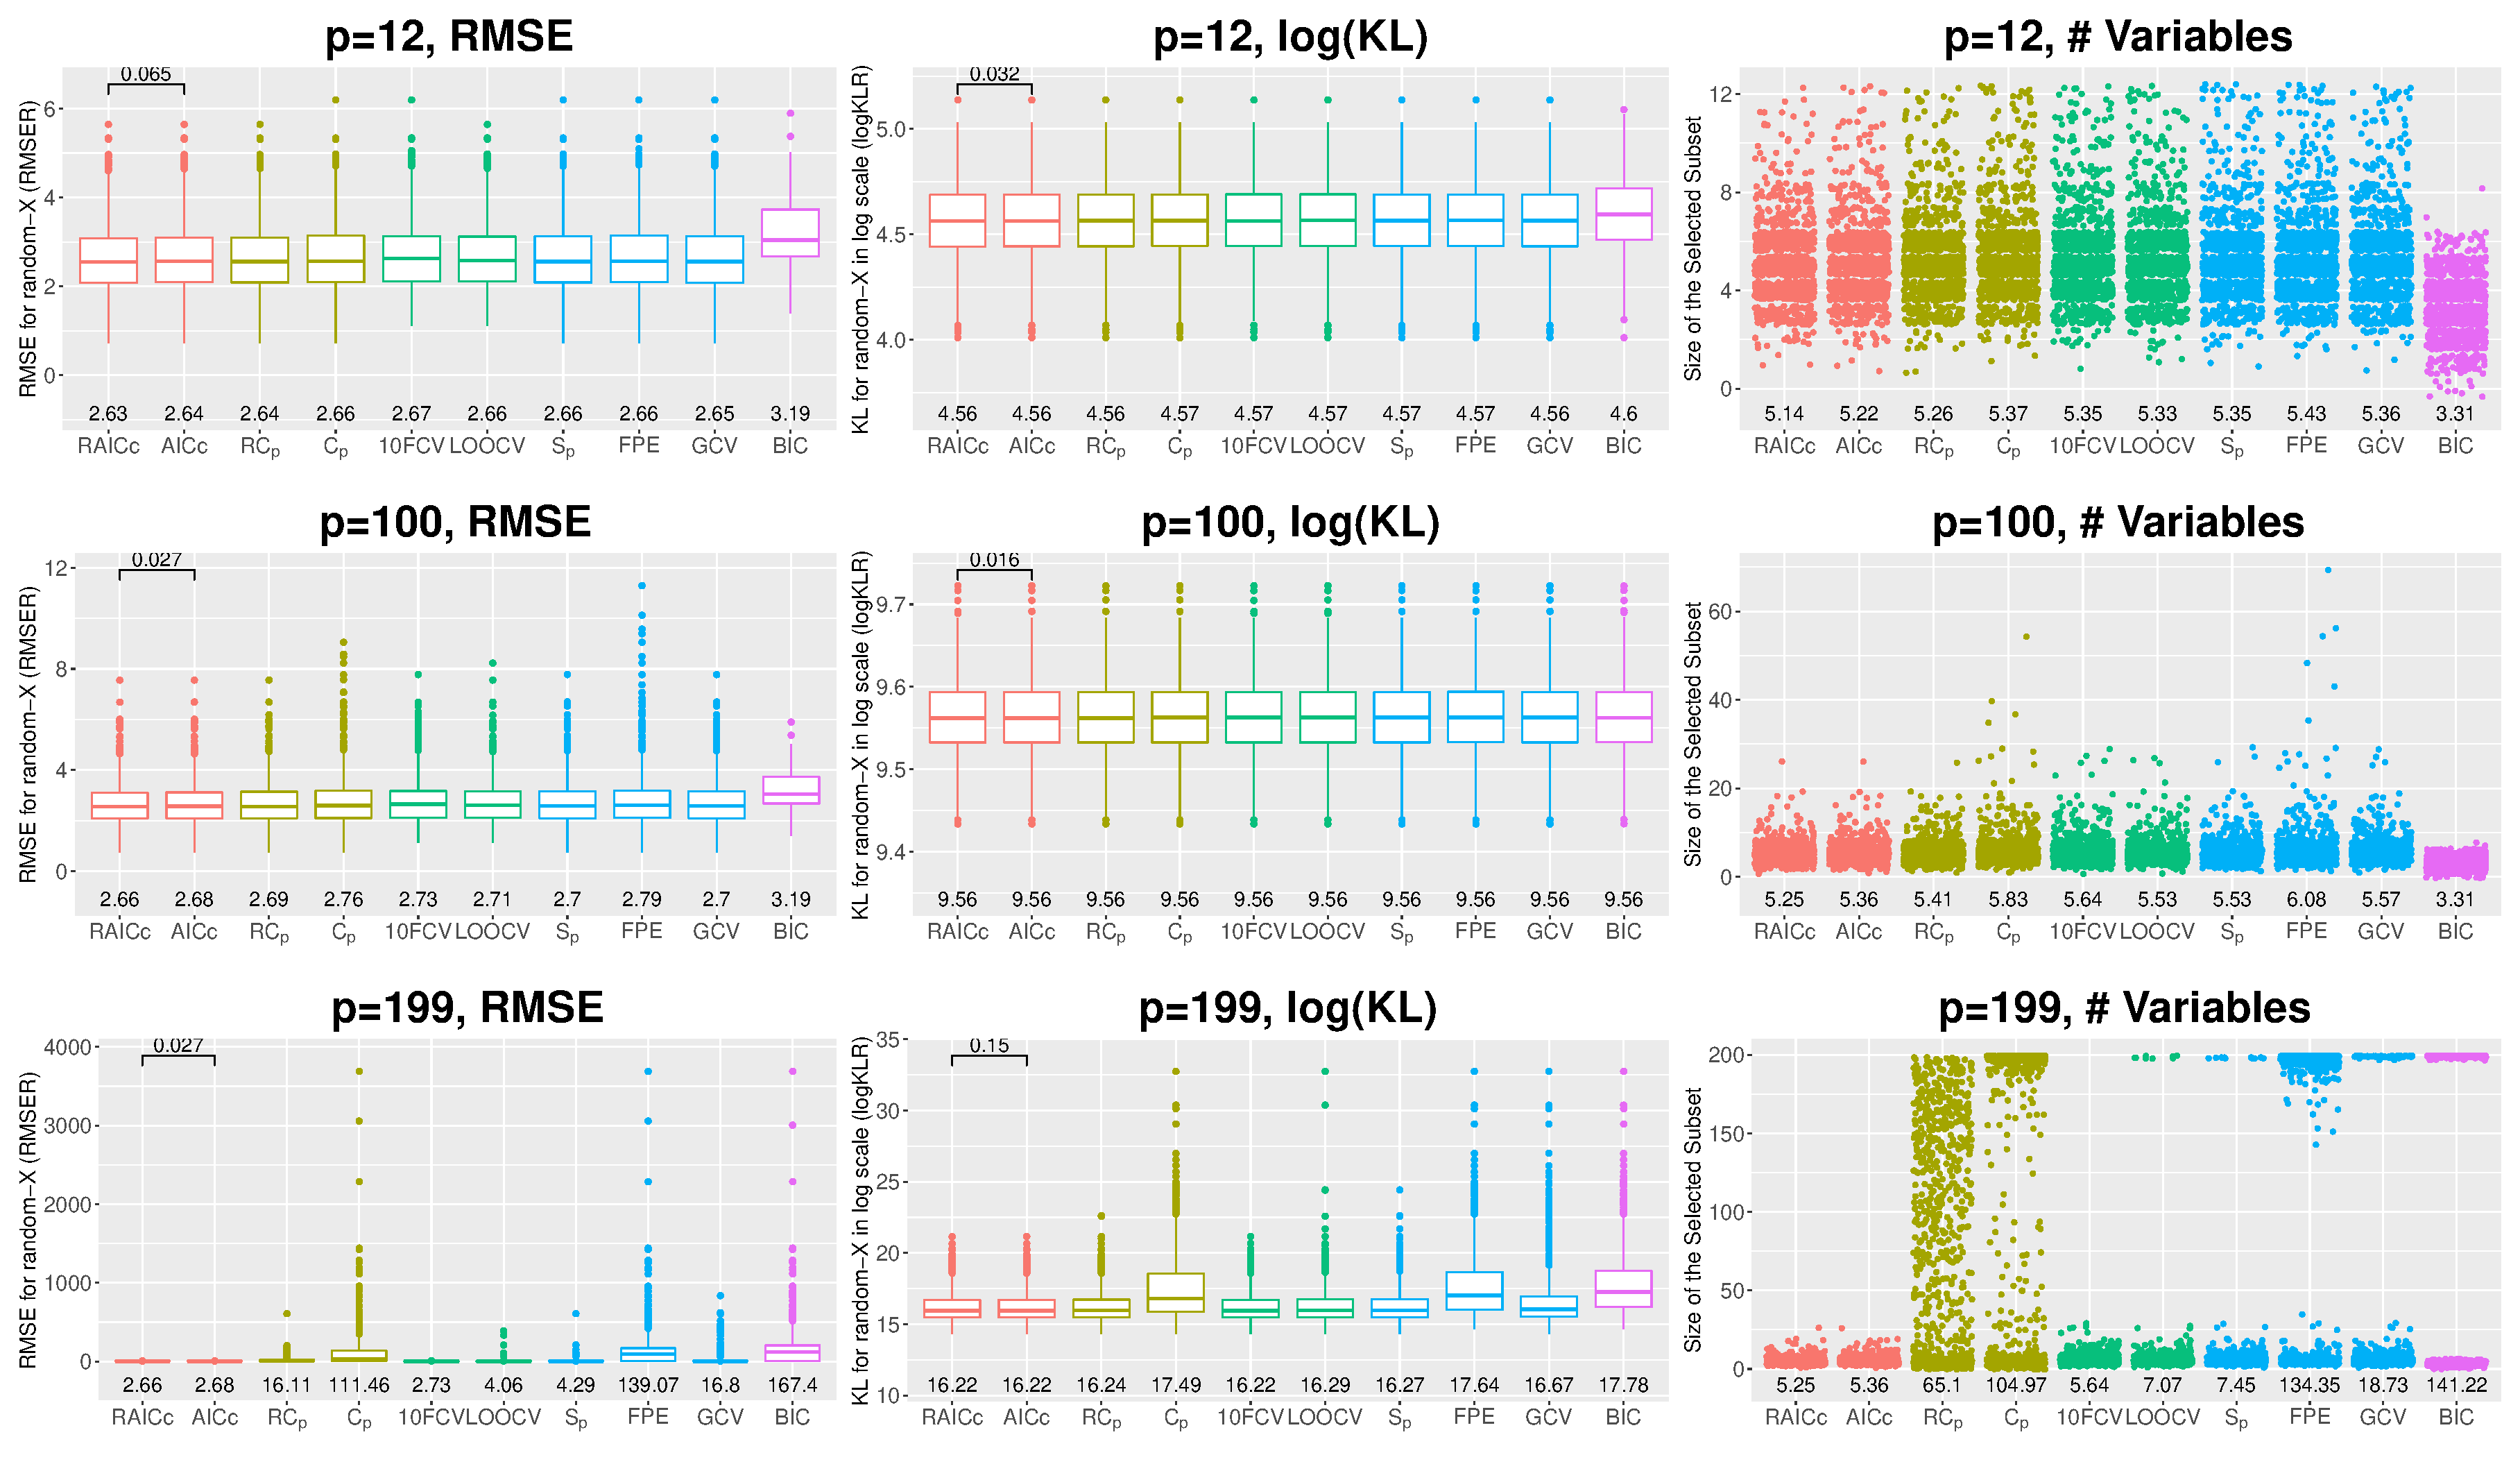
\includegraphics[width=\textwidth]{figures/supplement/randomx_VS-Ex1_n200_lsnr_rho0.eps}
\caption{VS-Ex1, $n=200$, low signal, $\rho=0$, and Random-X.}
\end{figure}
\begin{figure}[!ht]
\centering
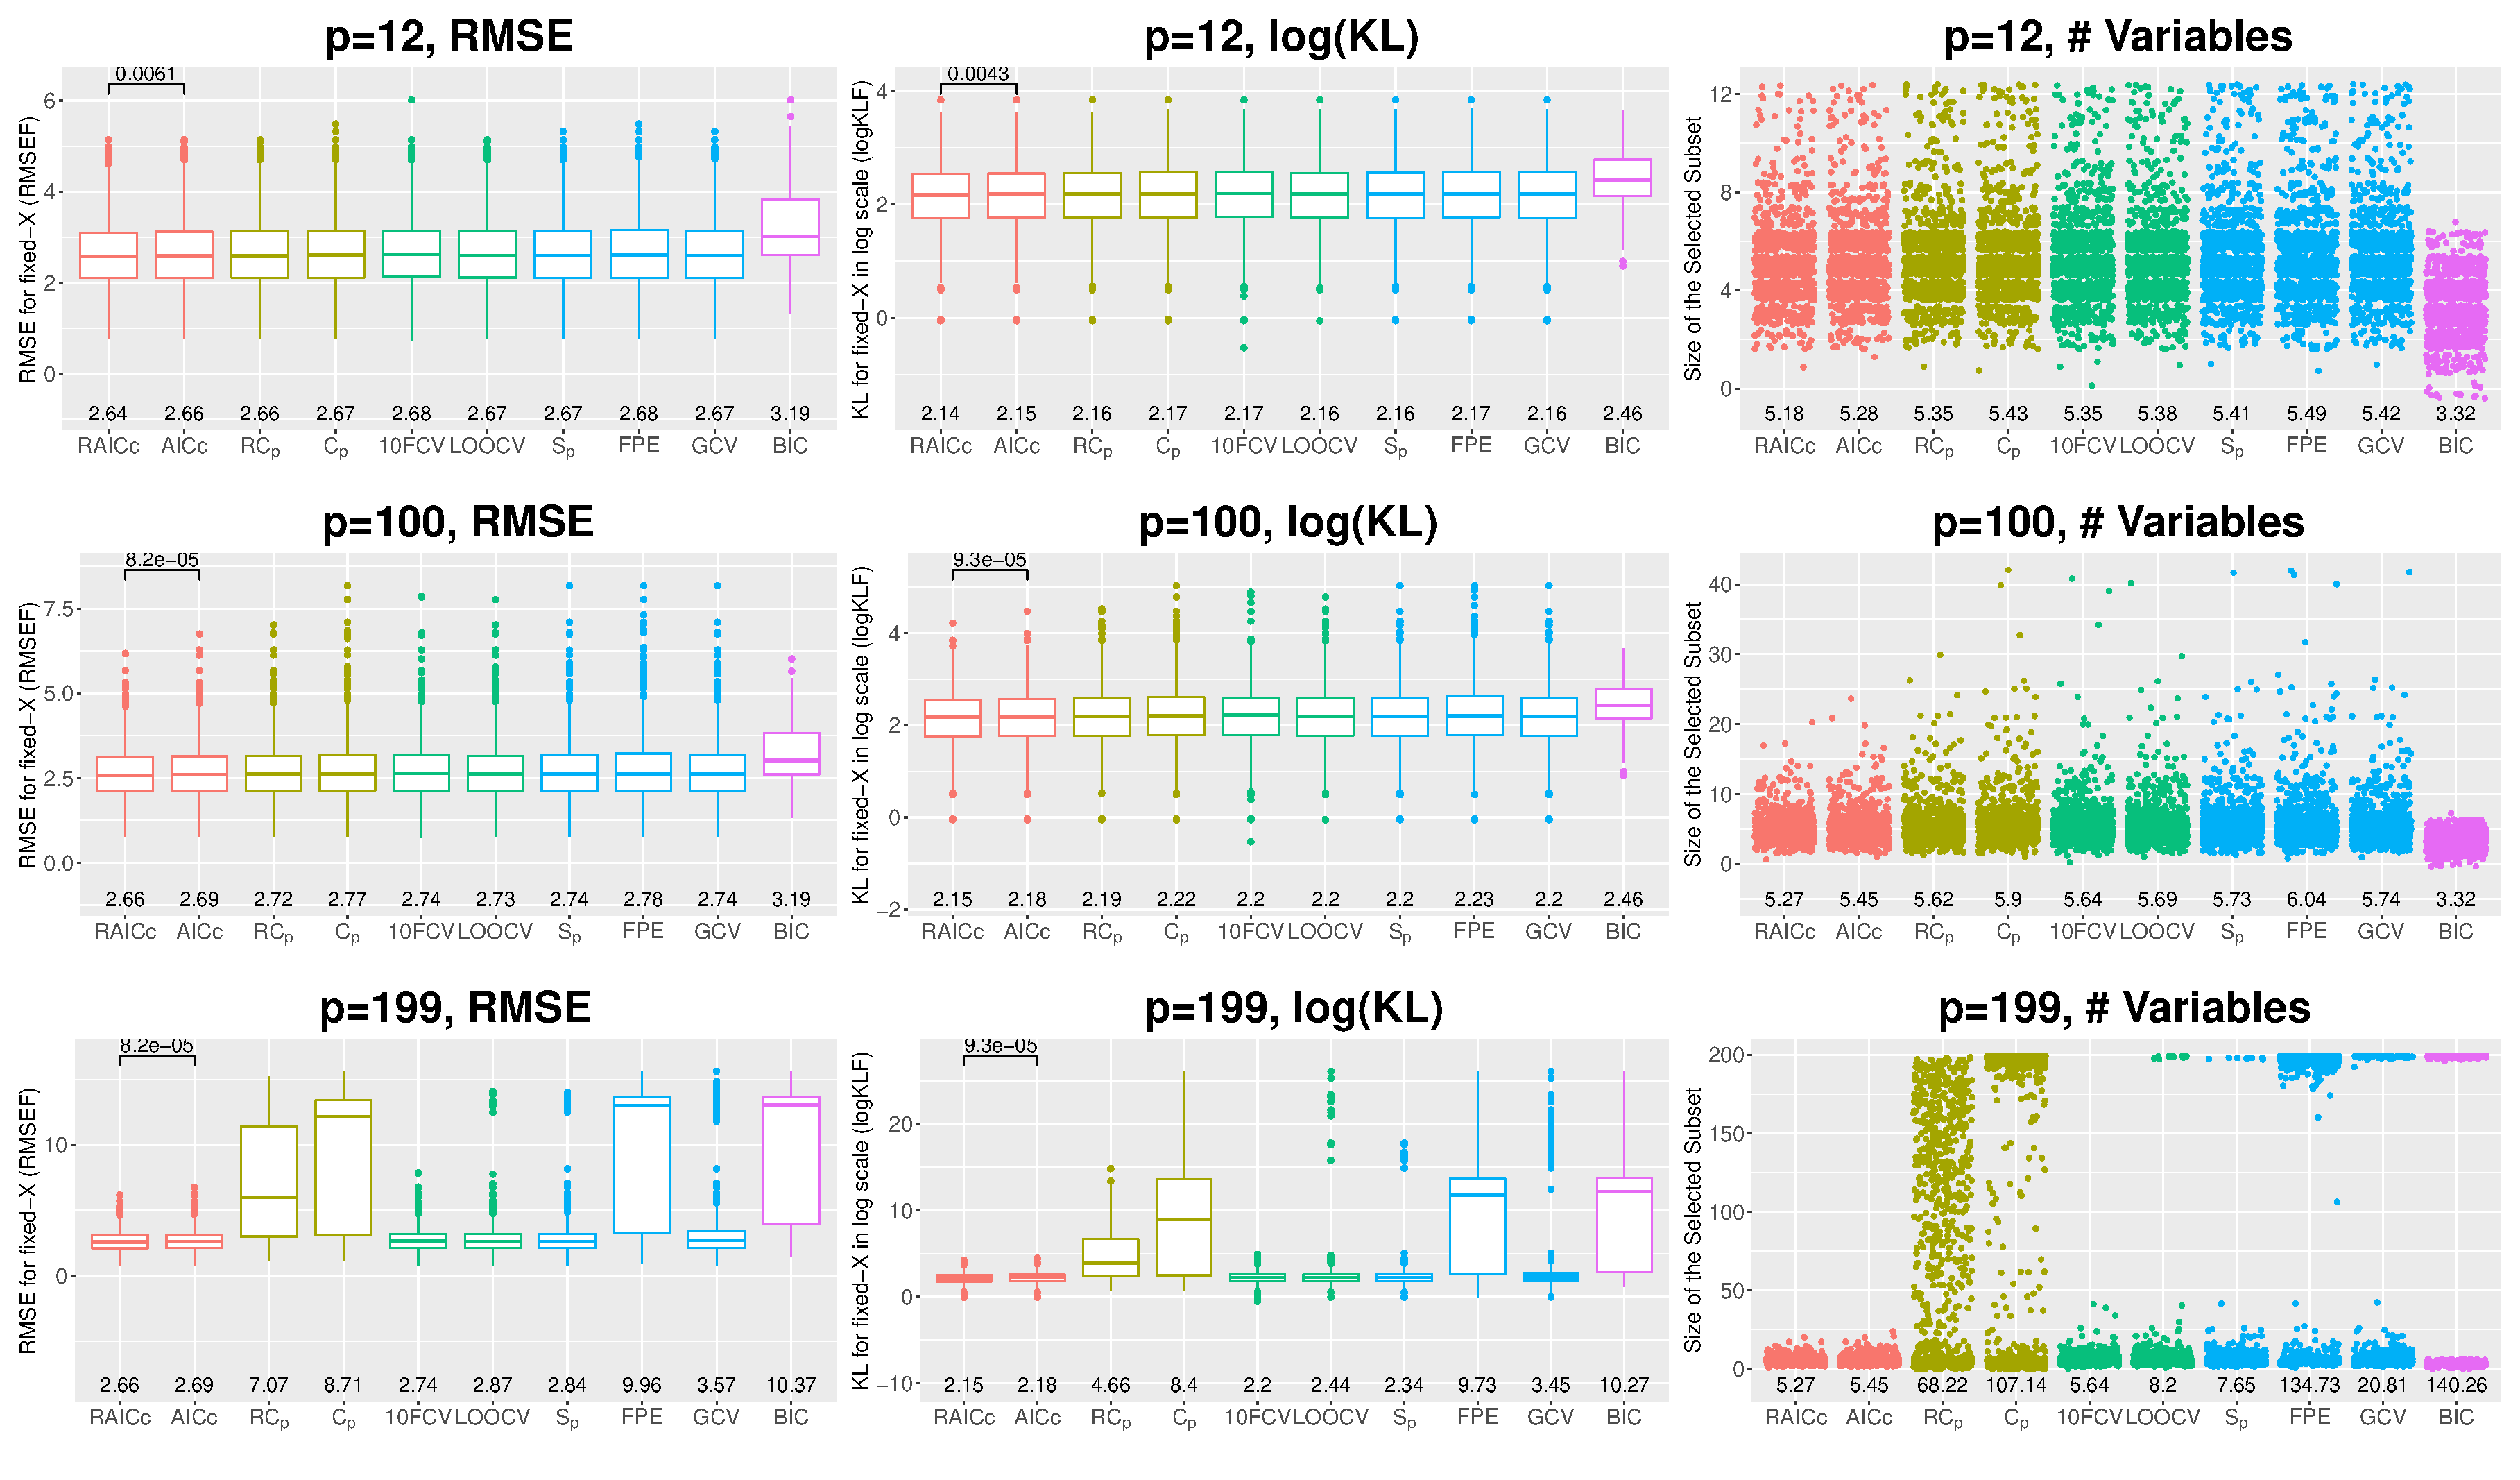
\includegraphics[width=\textwidth]{figures/supplement/fixedx_VS-Ex1_n200_lsnr_rho0.eps}
\caption{VS-Ex1, $n=200$, low signal, $\rho=0$, and Fixed-X.}
\end{figure}
\clearpage
\begin{figure}[!ht]
\centering
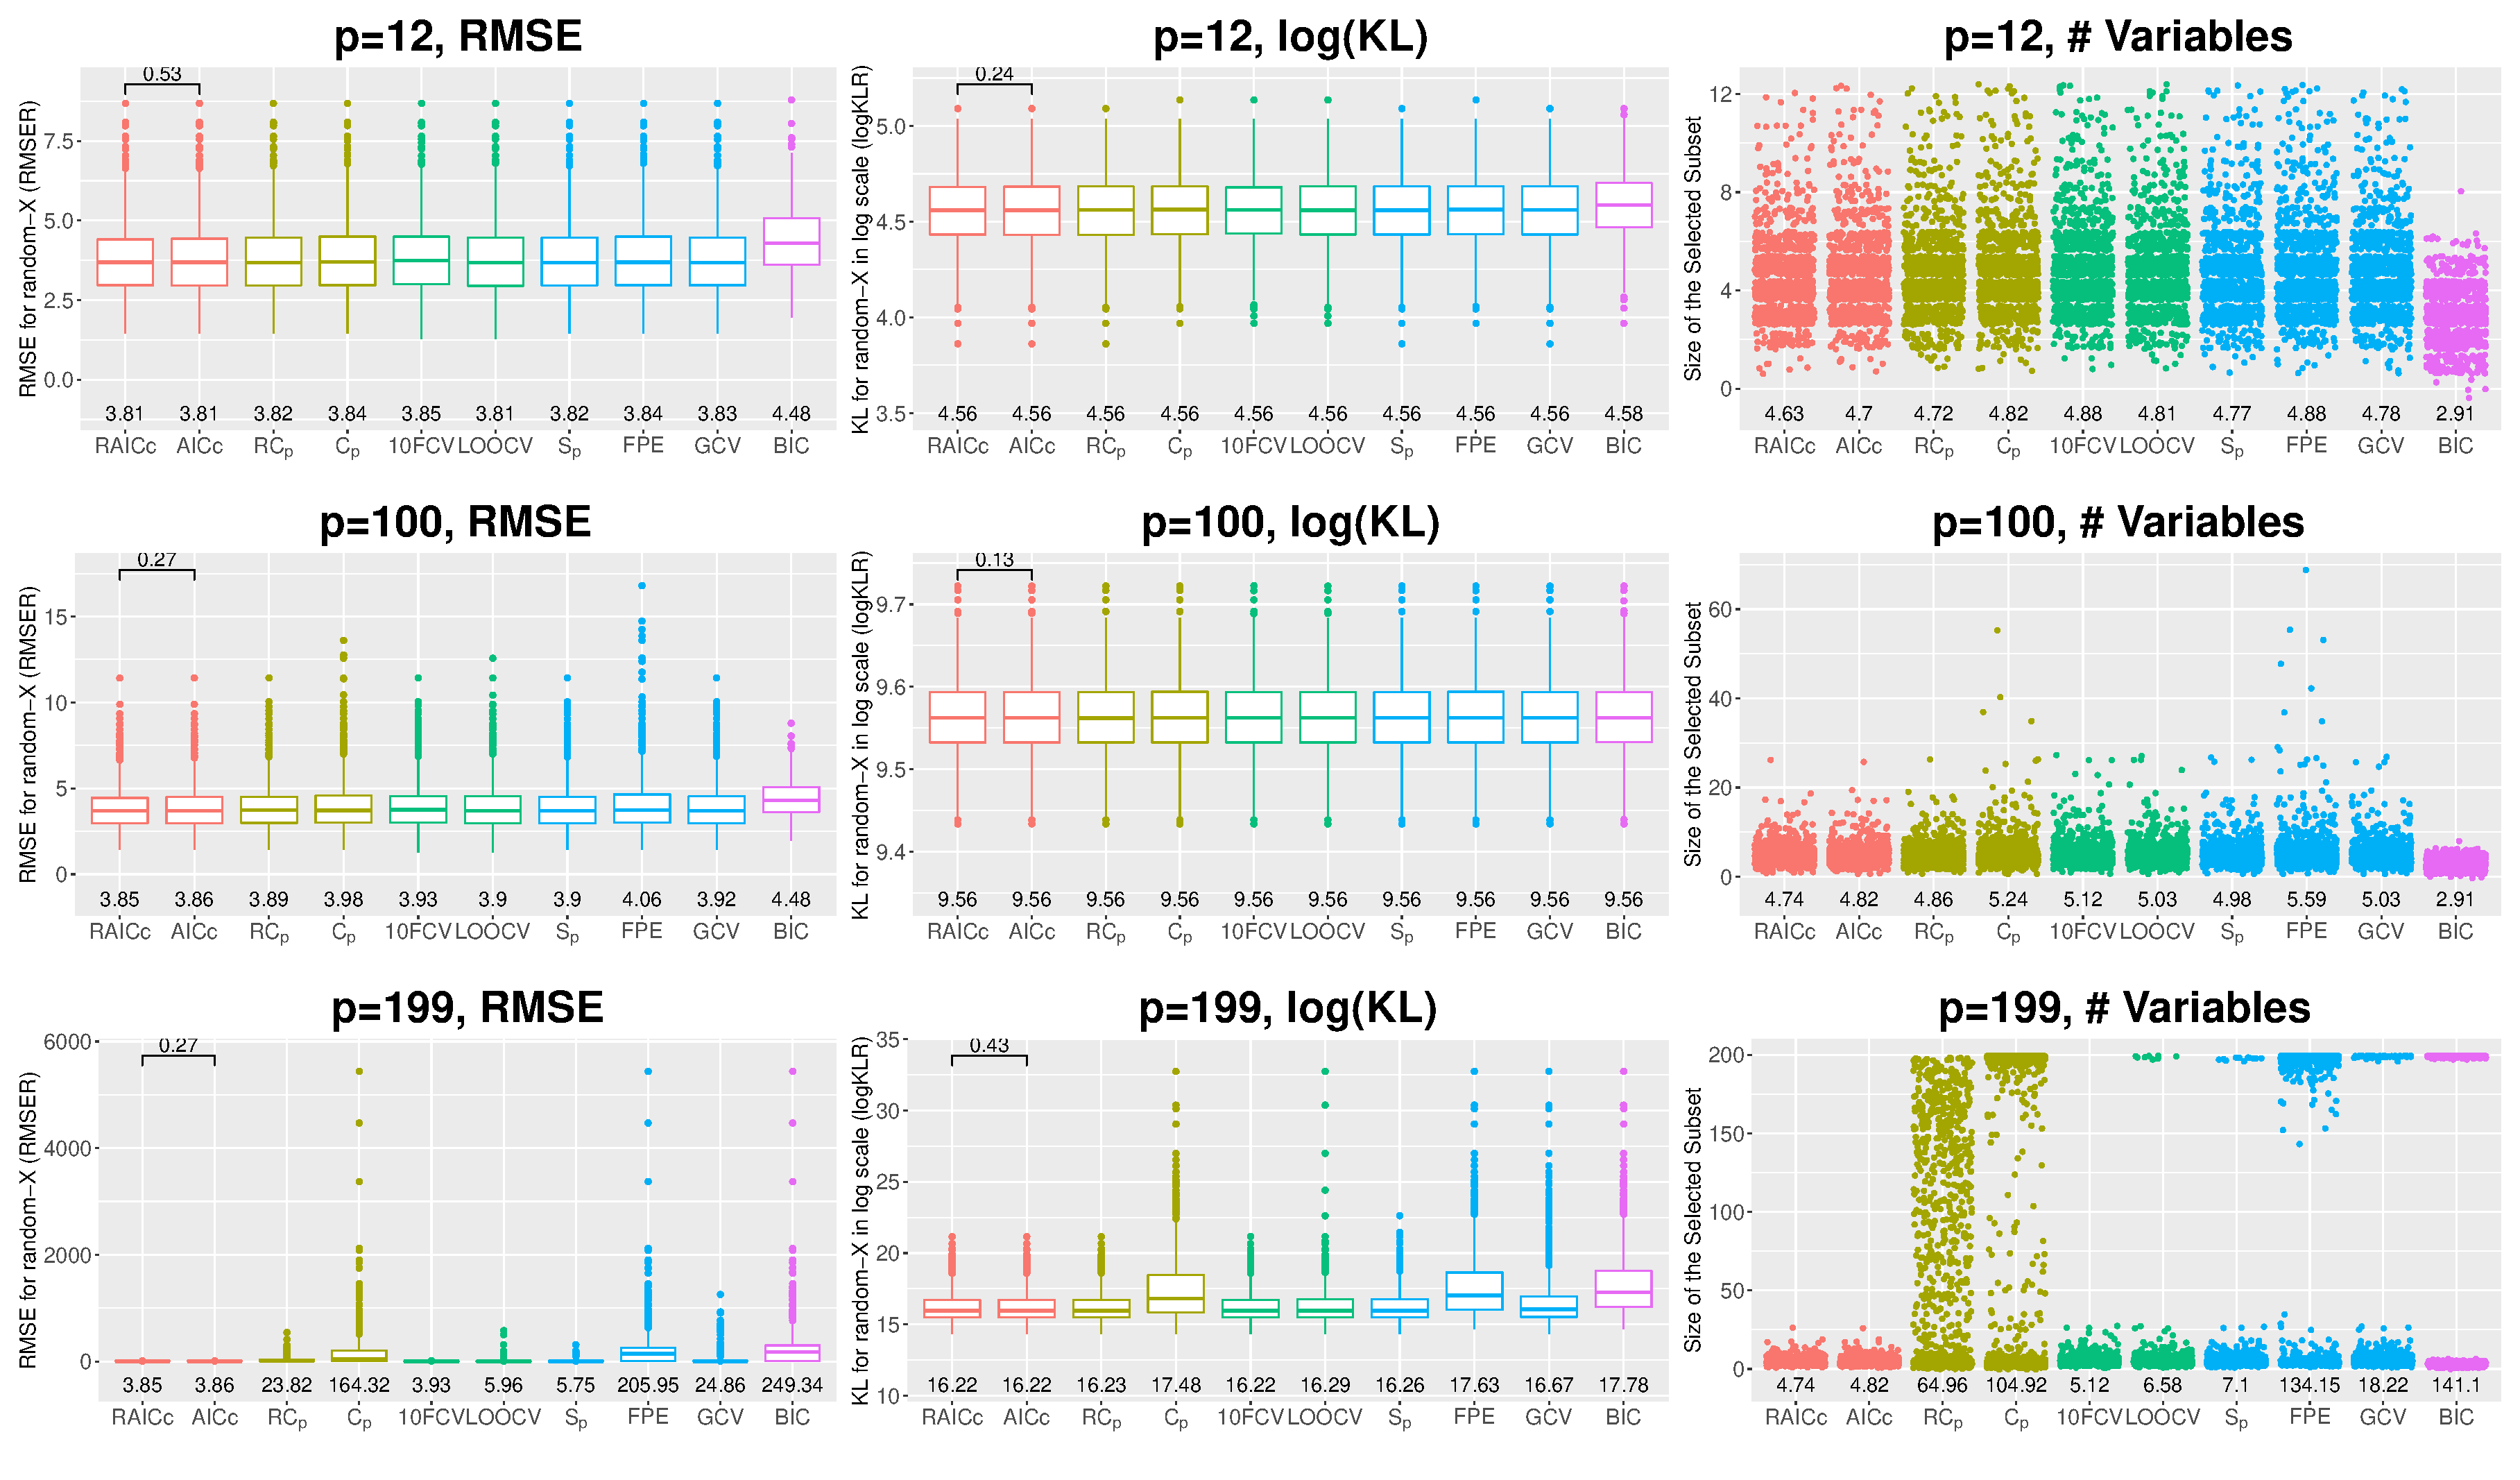
\includegraphics[width=\textwidth]{figures/supplement/randomx_VS-Ex1_n200_lsnr_rho05.eps}
\caption{VS-Ex1, $n=200$, low signal, $\rho=0.5$, and Random-X.}
\end{figure}
\begin{figure}[!ht]
\centering
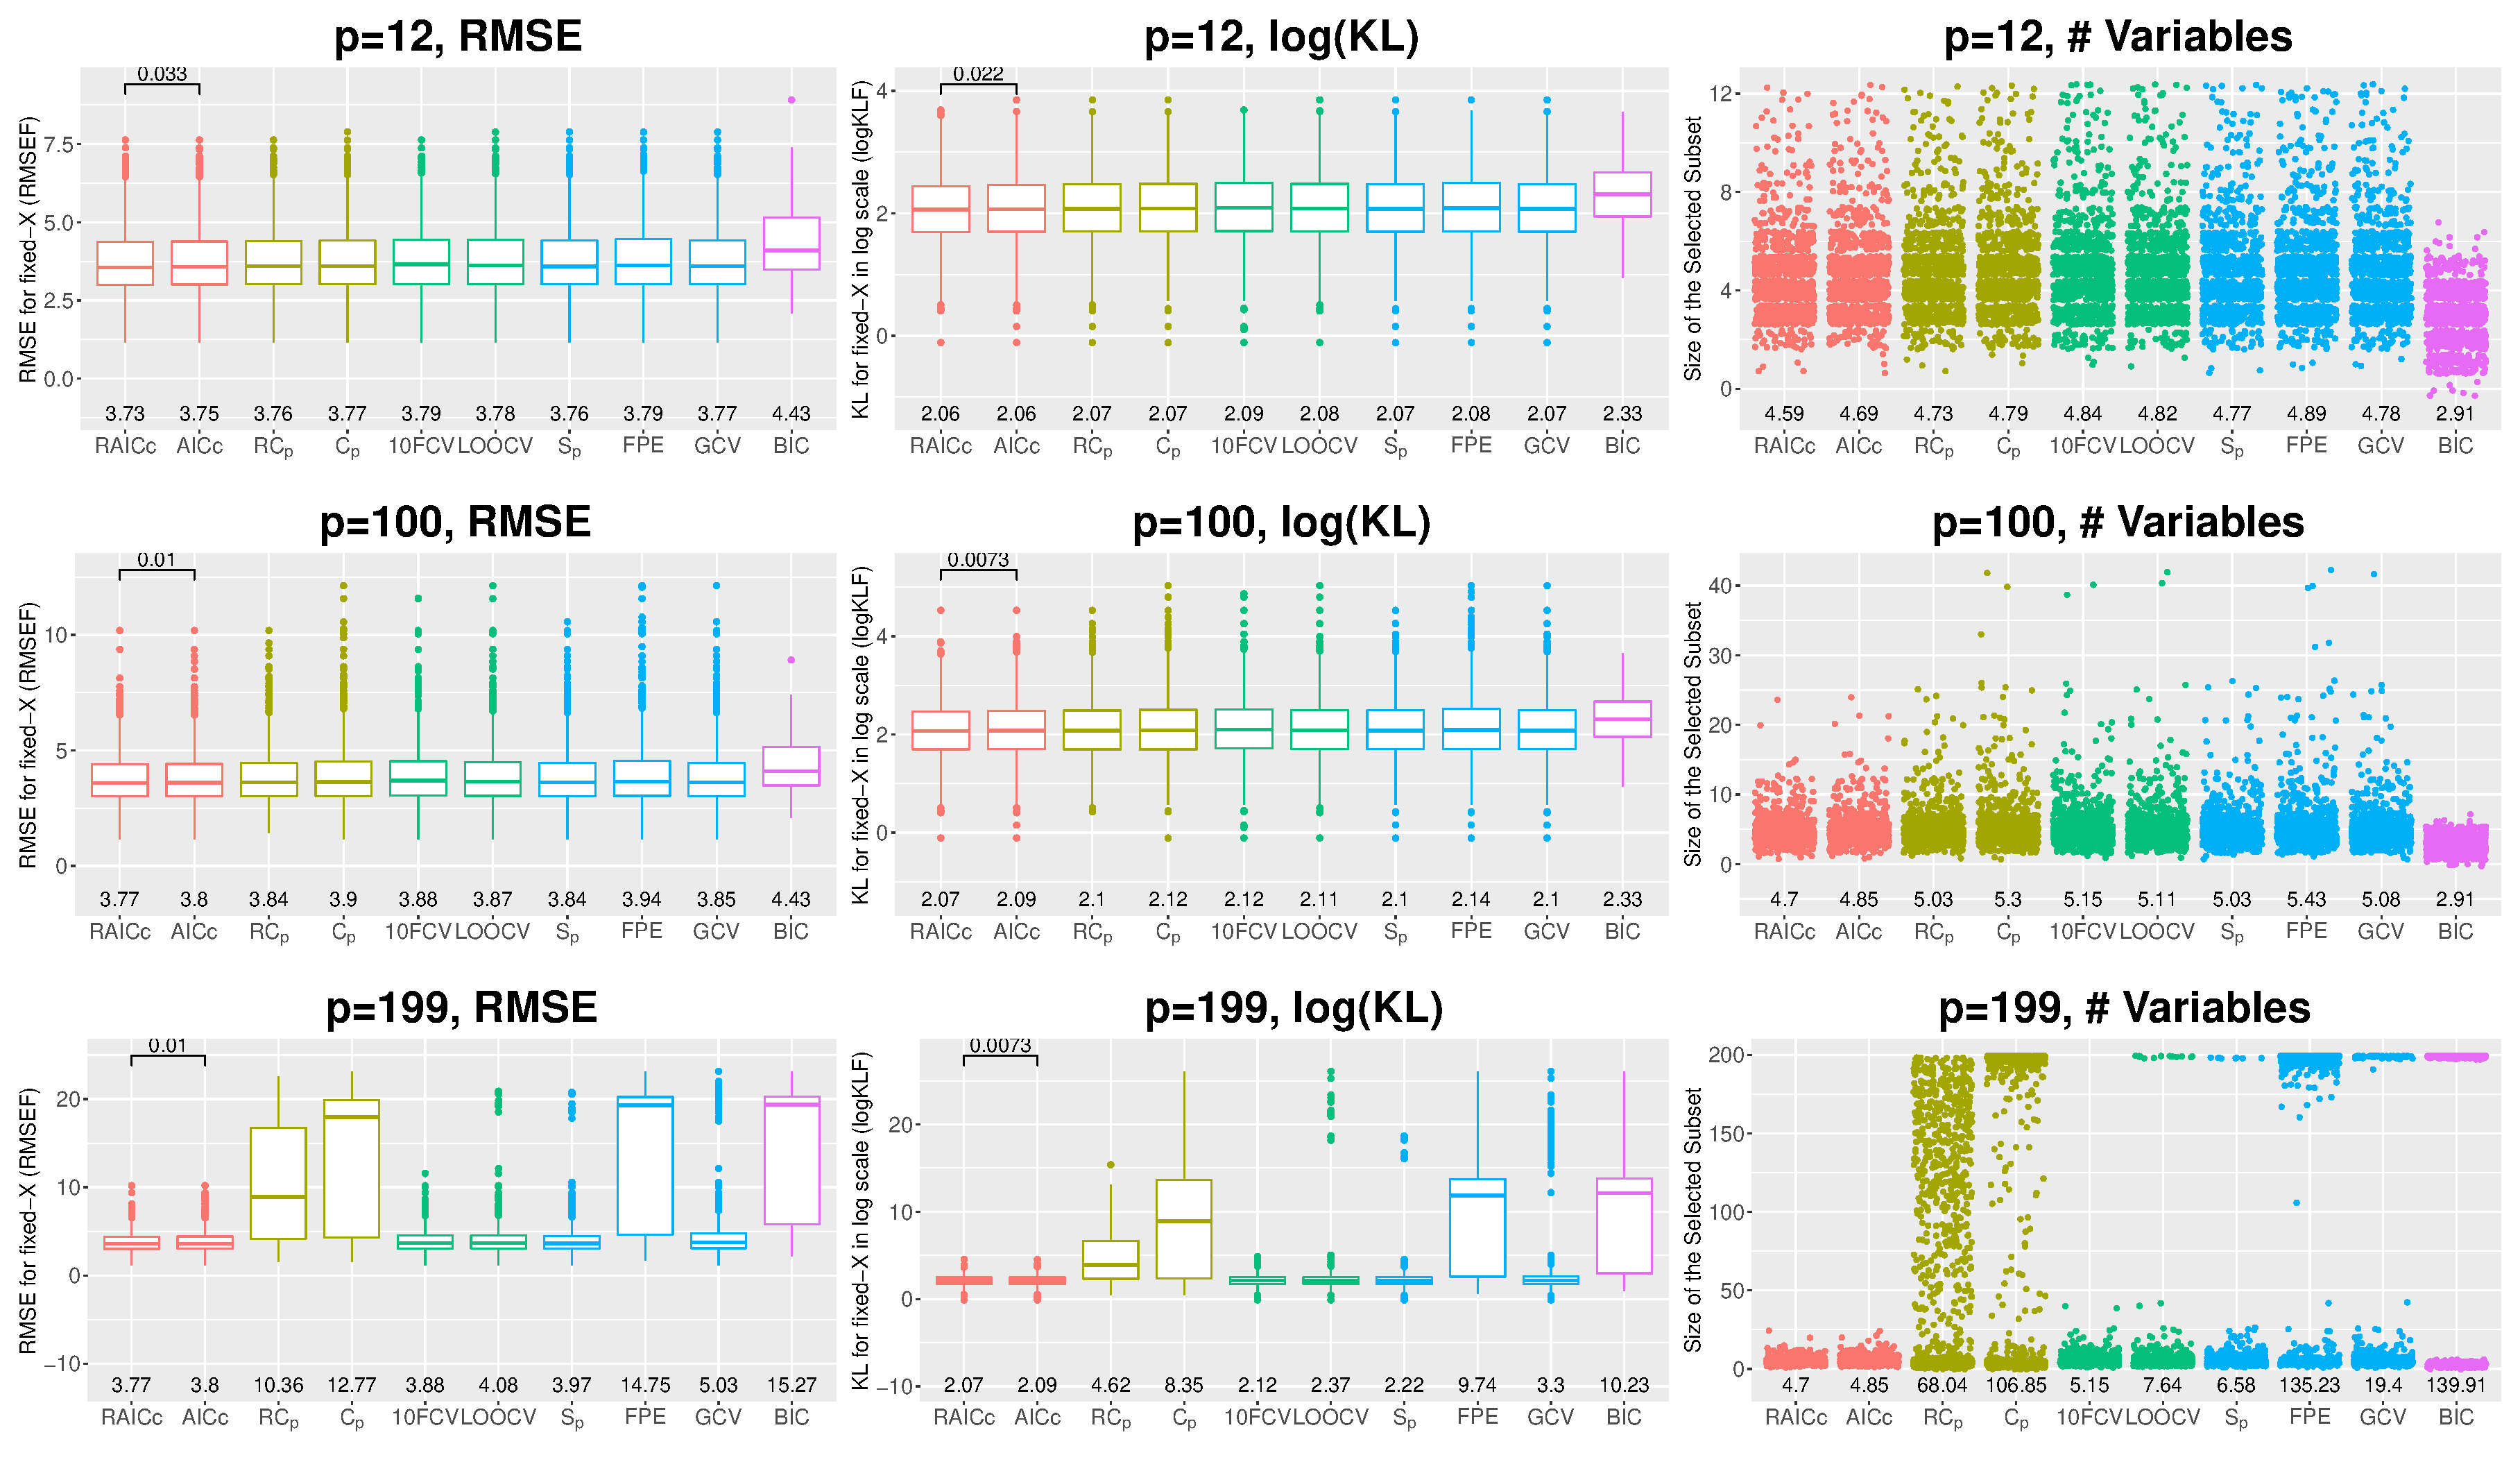
\includegraphics[width=\textwidth]{figures/supplement/fixedx_VS-Ex1_n200_lsnr_rho05.eps}
\caption{VS-Ex1, $n=200$, low signal, $\rho=0.5$, and Fixed-X.}
\end{figure}
\clearpage
\begin{figure}[!ht]
\centering
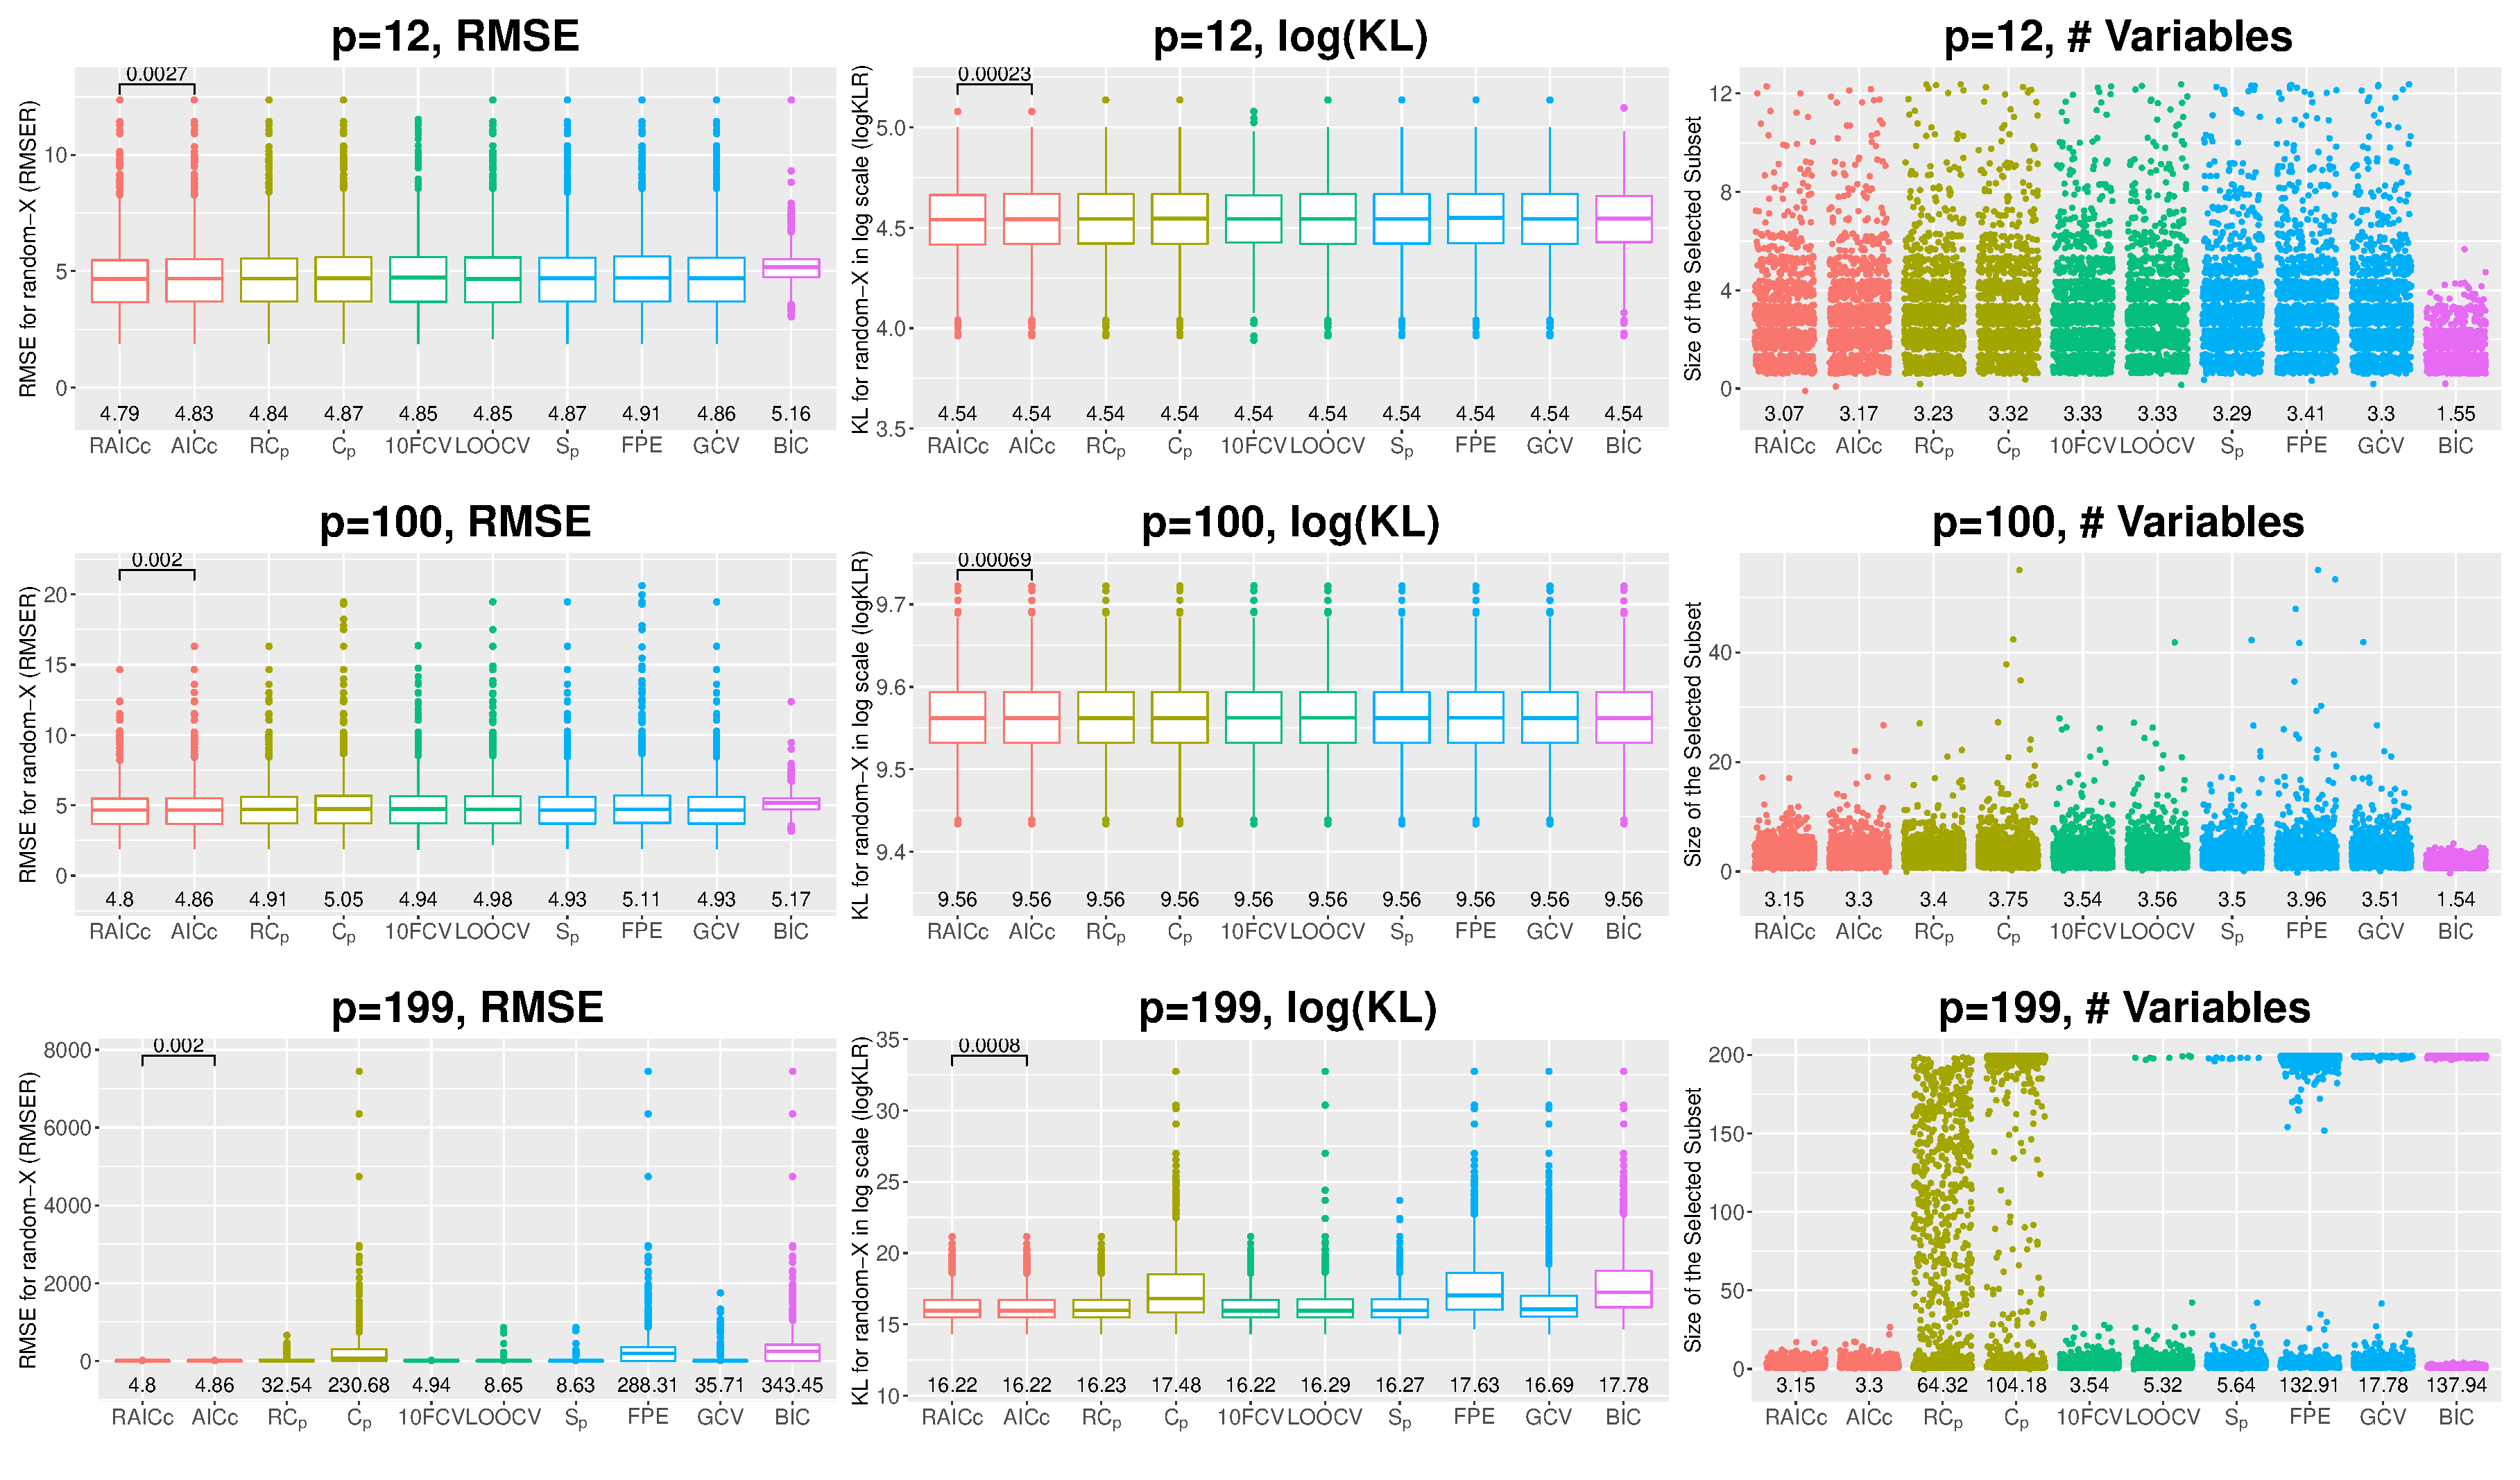
\includegraphics[width=\textwidth]{figures/supplement/randomx_VS-Ex1_n200_lsnr_rho09.eps}
\caption{VS-Ex1, $n=200$, low signal, $\rho=0.9$, and Random-X.}
\end{figure}
\begin{figure}[!ht]
\centering
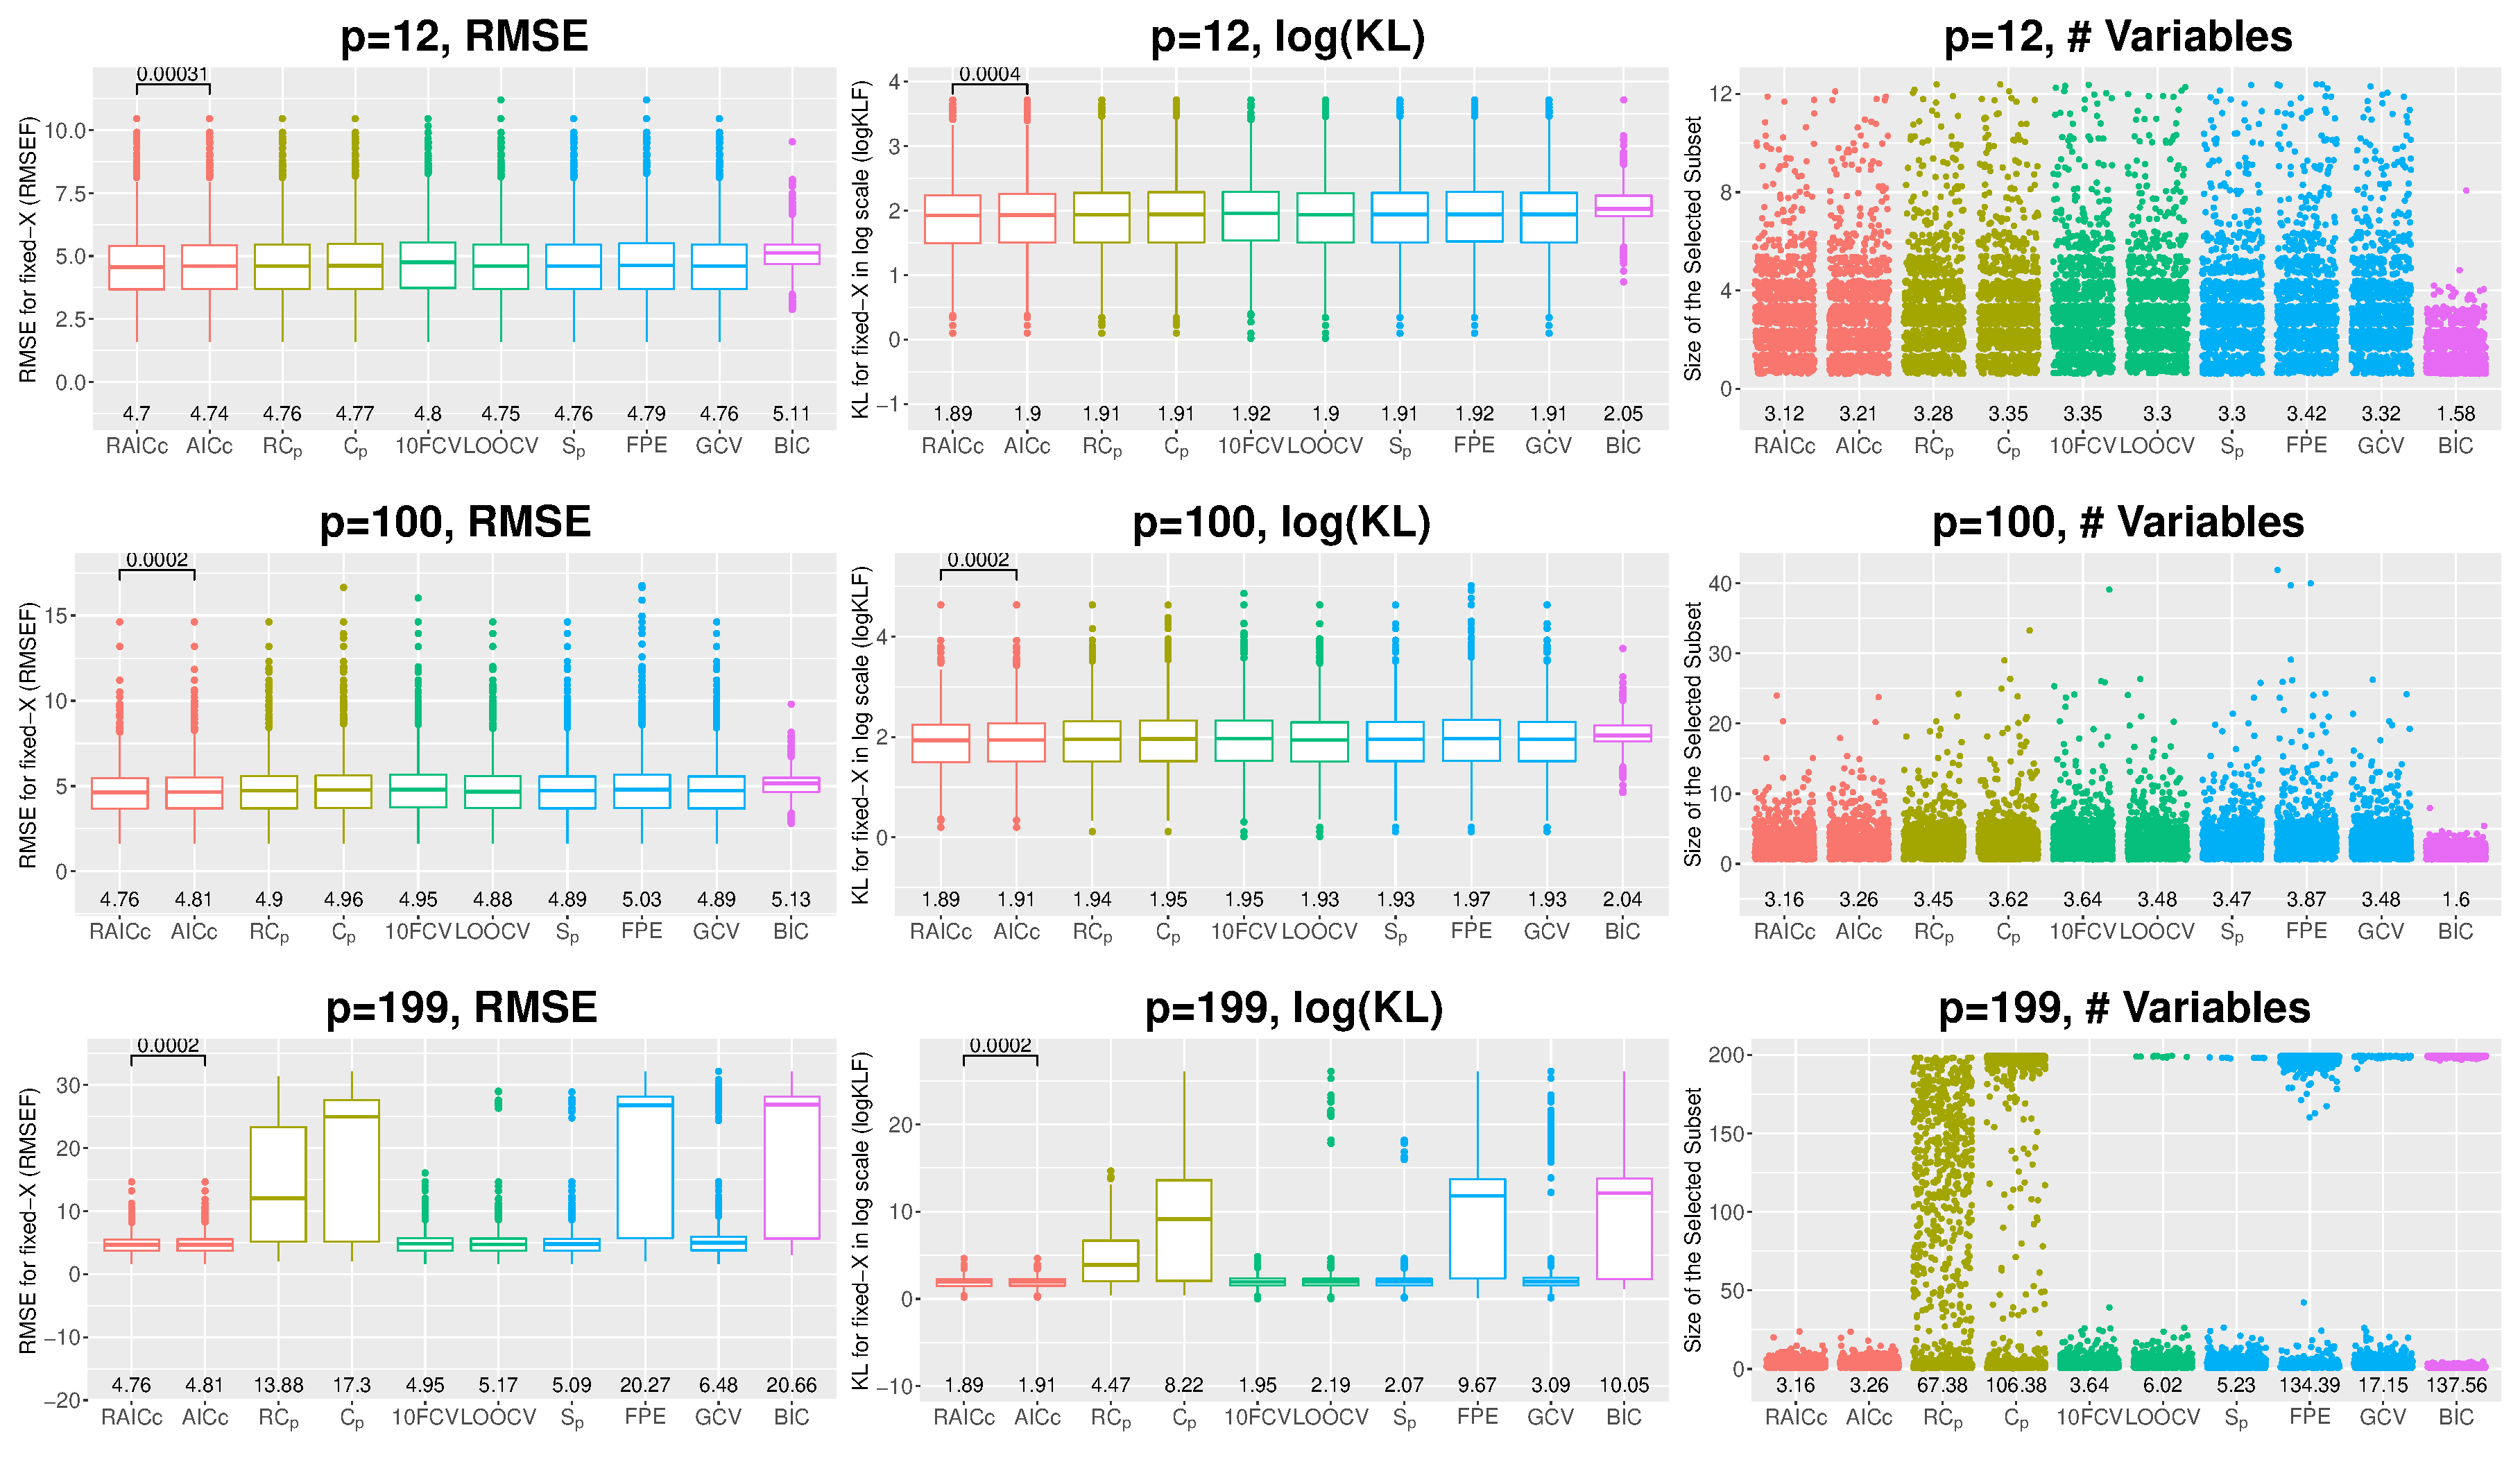
\includegraphics[width=\textwidth]{figures/supplement/fixedx_VS-Ex1_n200_lsnr_rho09.eps}
\caption{VS-Ex1, $n=200$, low signal, $\rho=0.9$, and Fixed-X.}
\end{figure}
\clearpage
\begin{figure}[!ht]
\centering
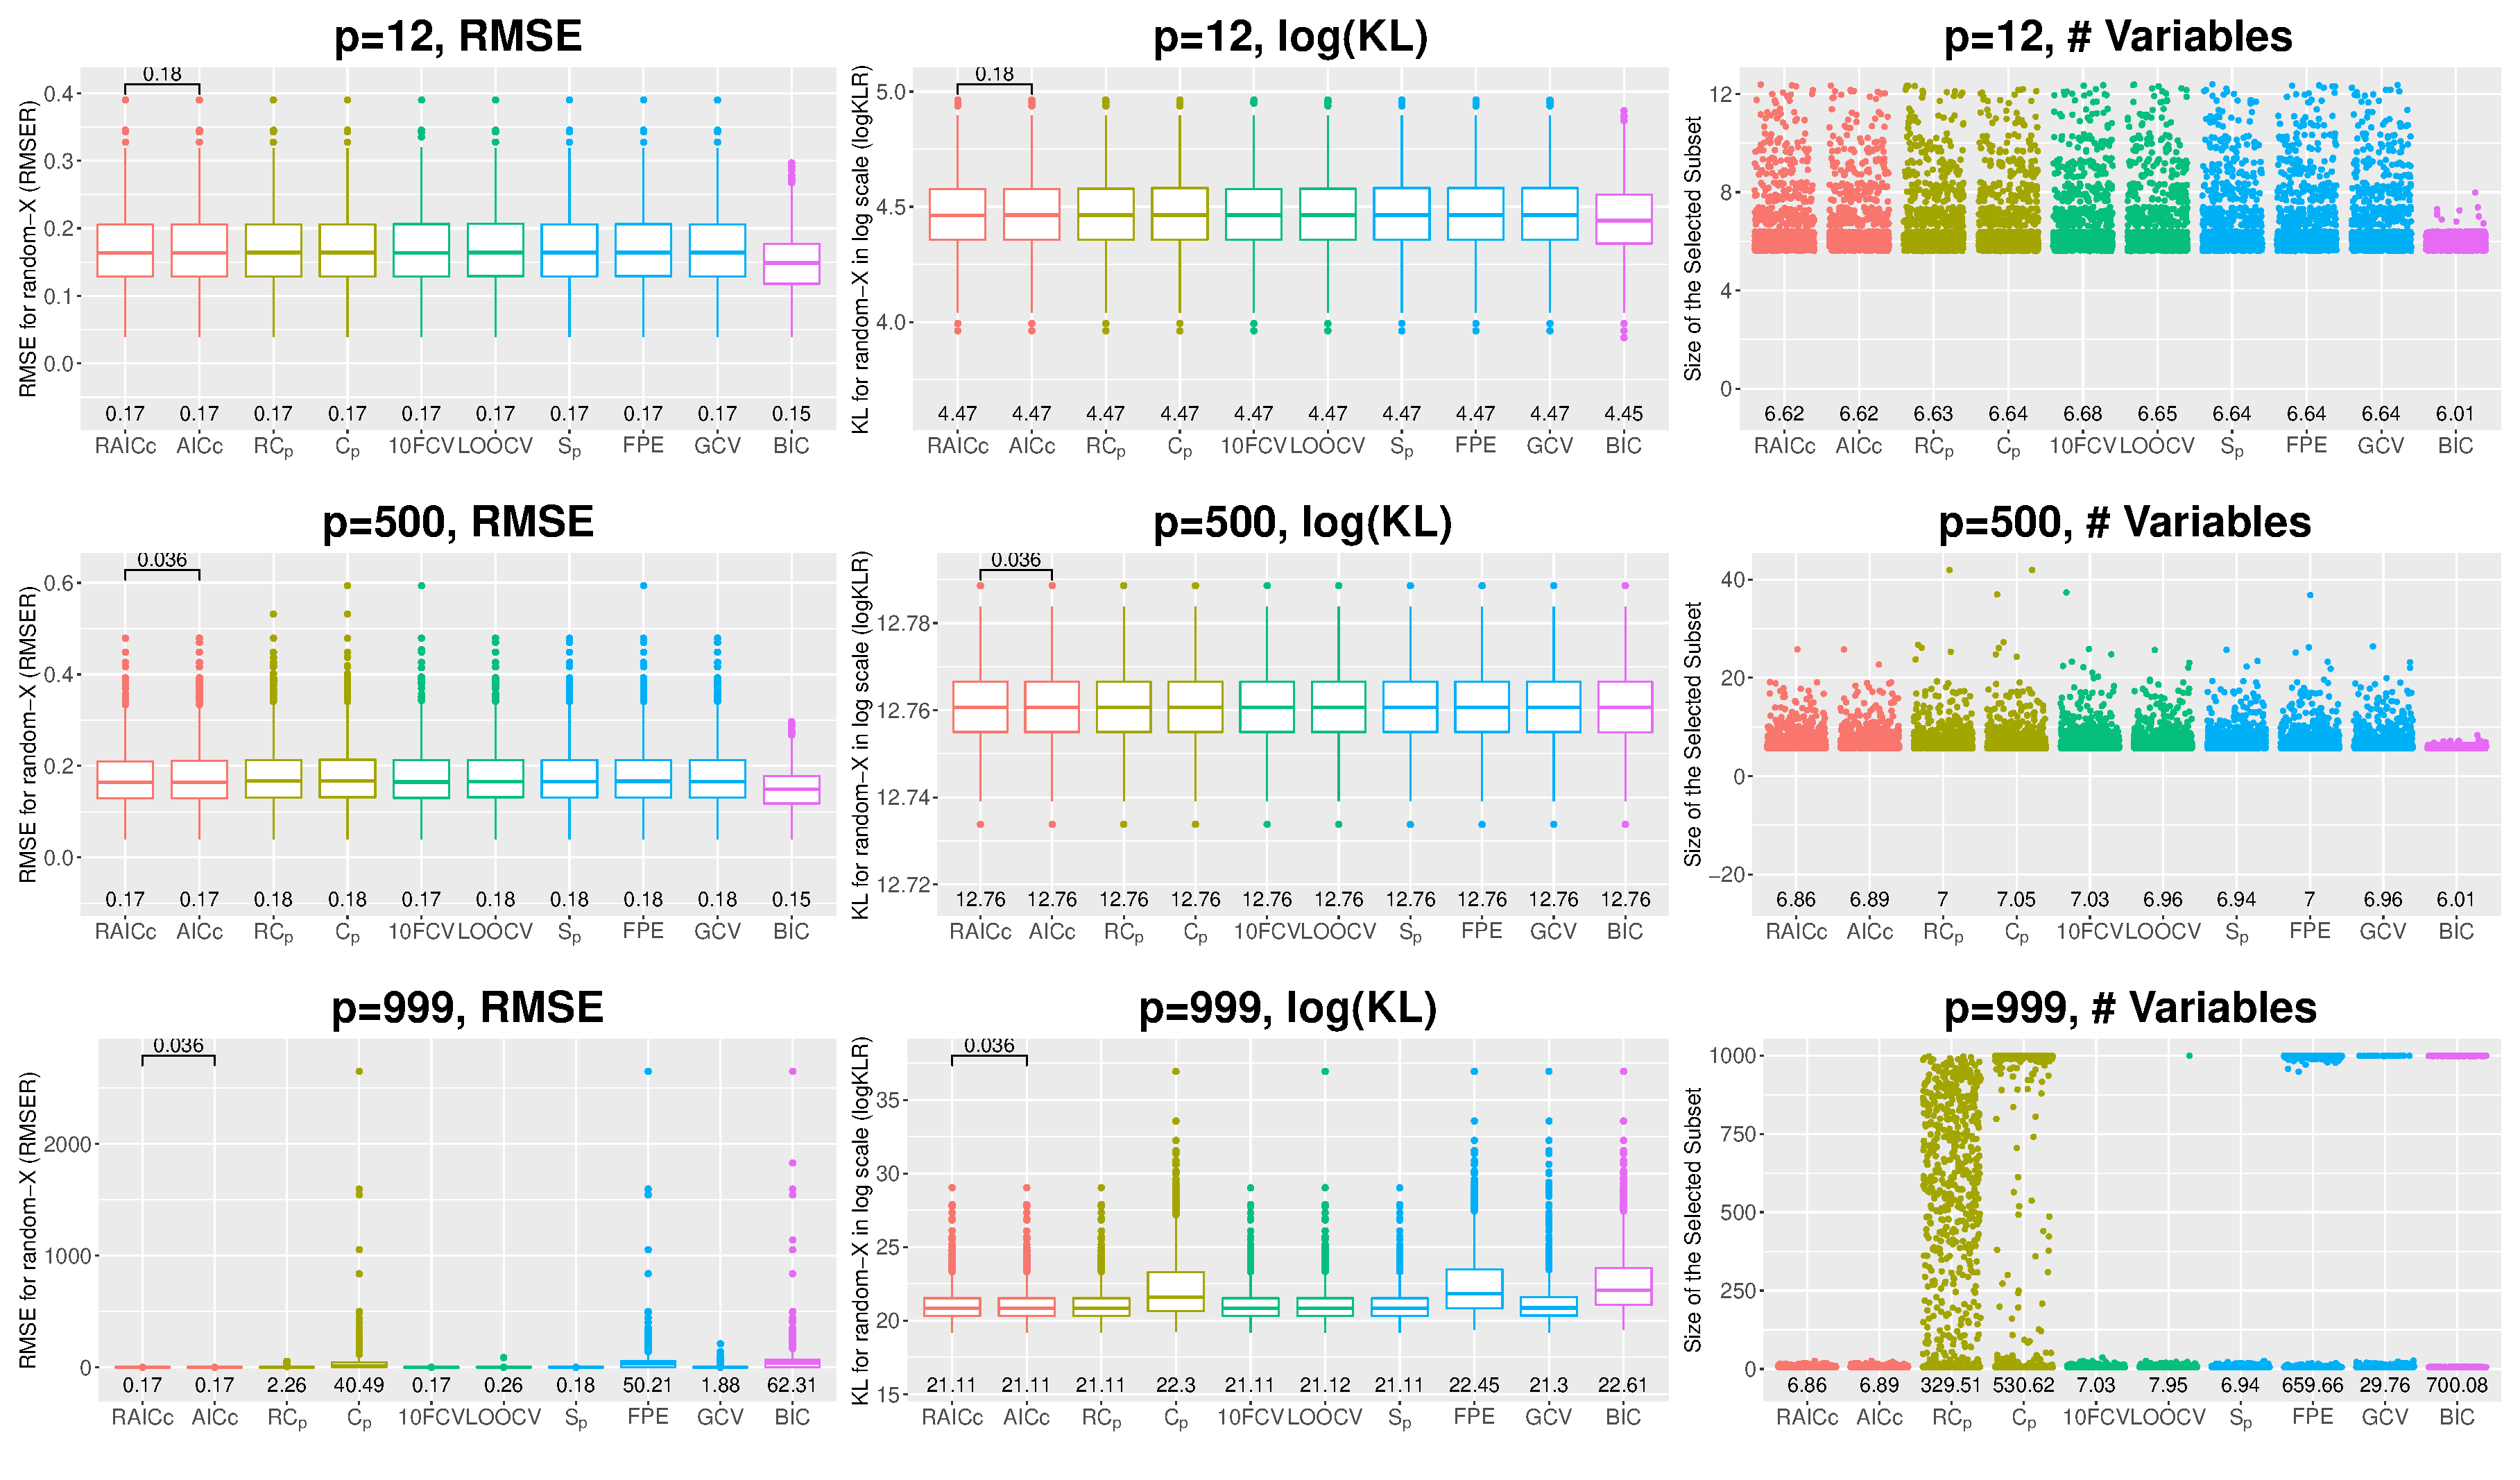
\includegraphics[width=\textwidth]{figures/supplement/randomx_VS-Ex1_n1000_hsnr_rho0.eps}
\caption{VS-Ex1, $n=1000$, high signal, $\rho=0$, and Random-X.}
\end{figure}
\begin{figure}[!ht]
\centering
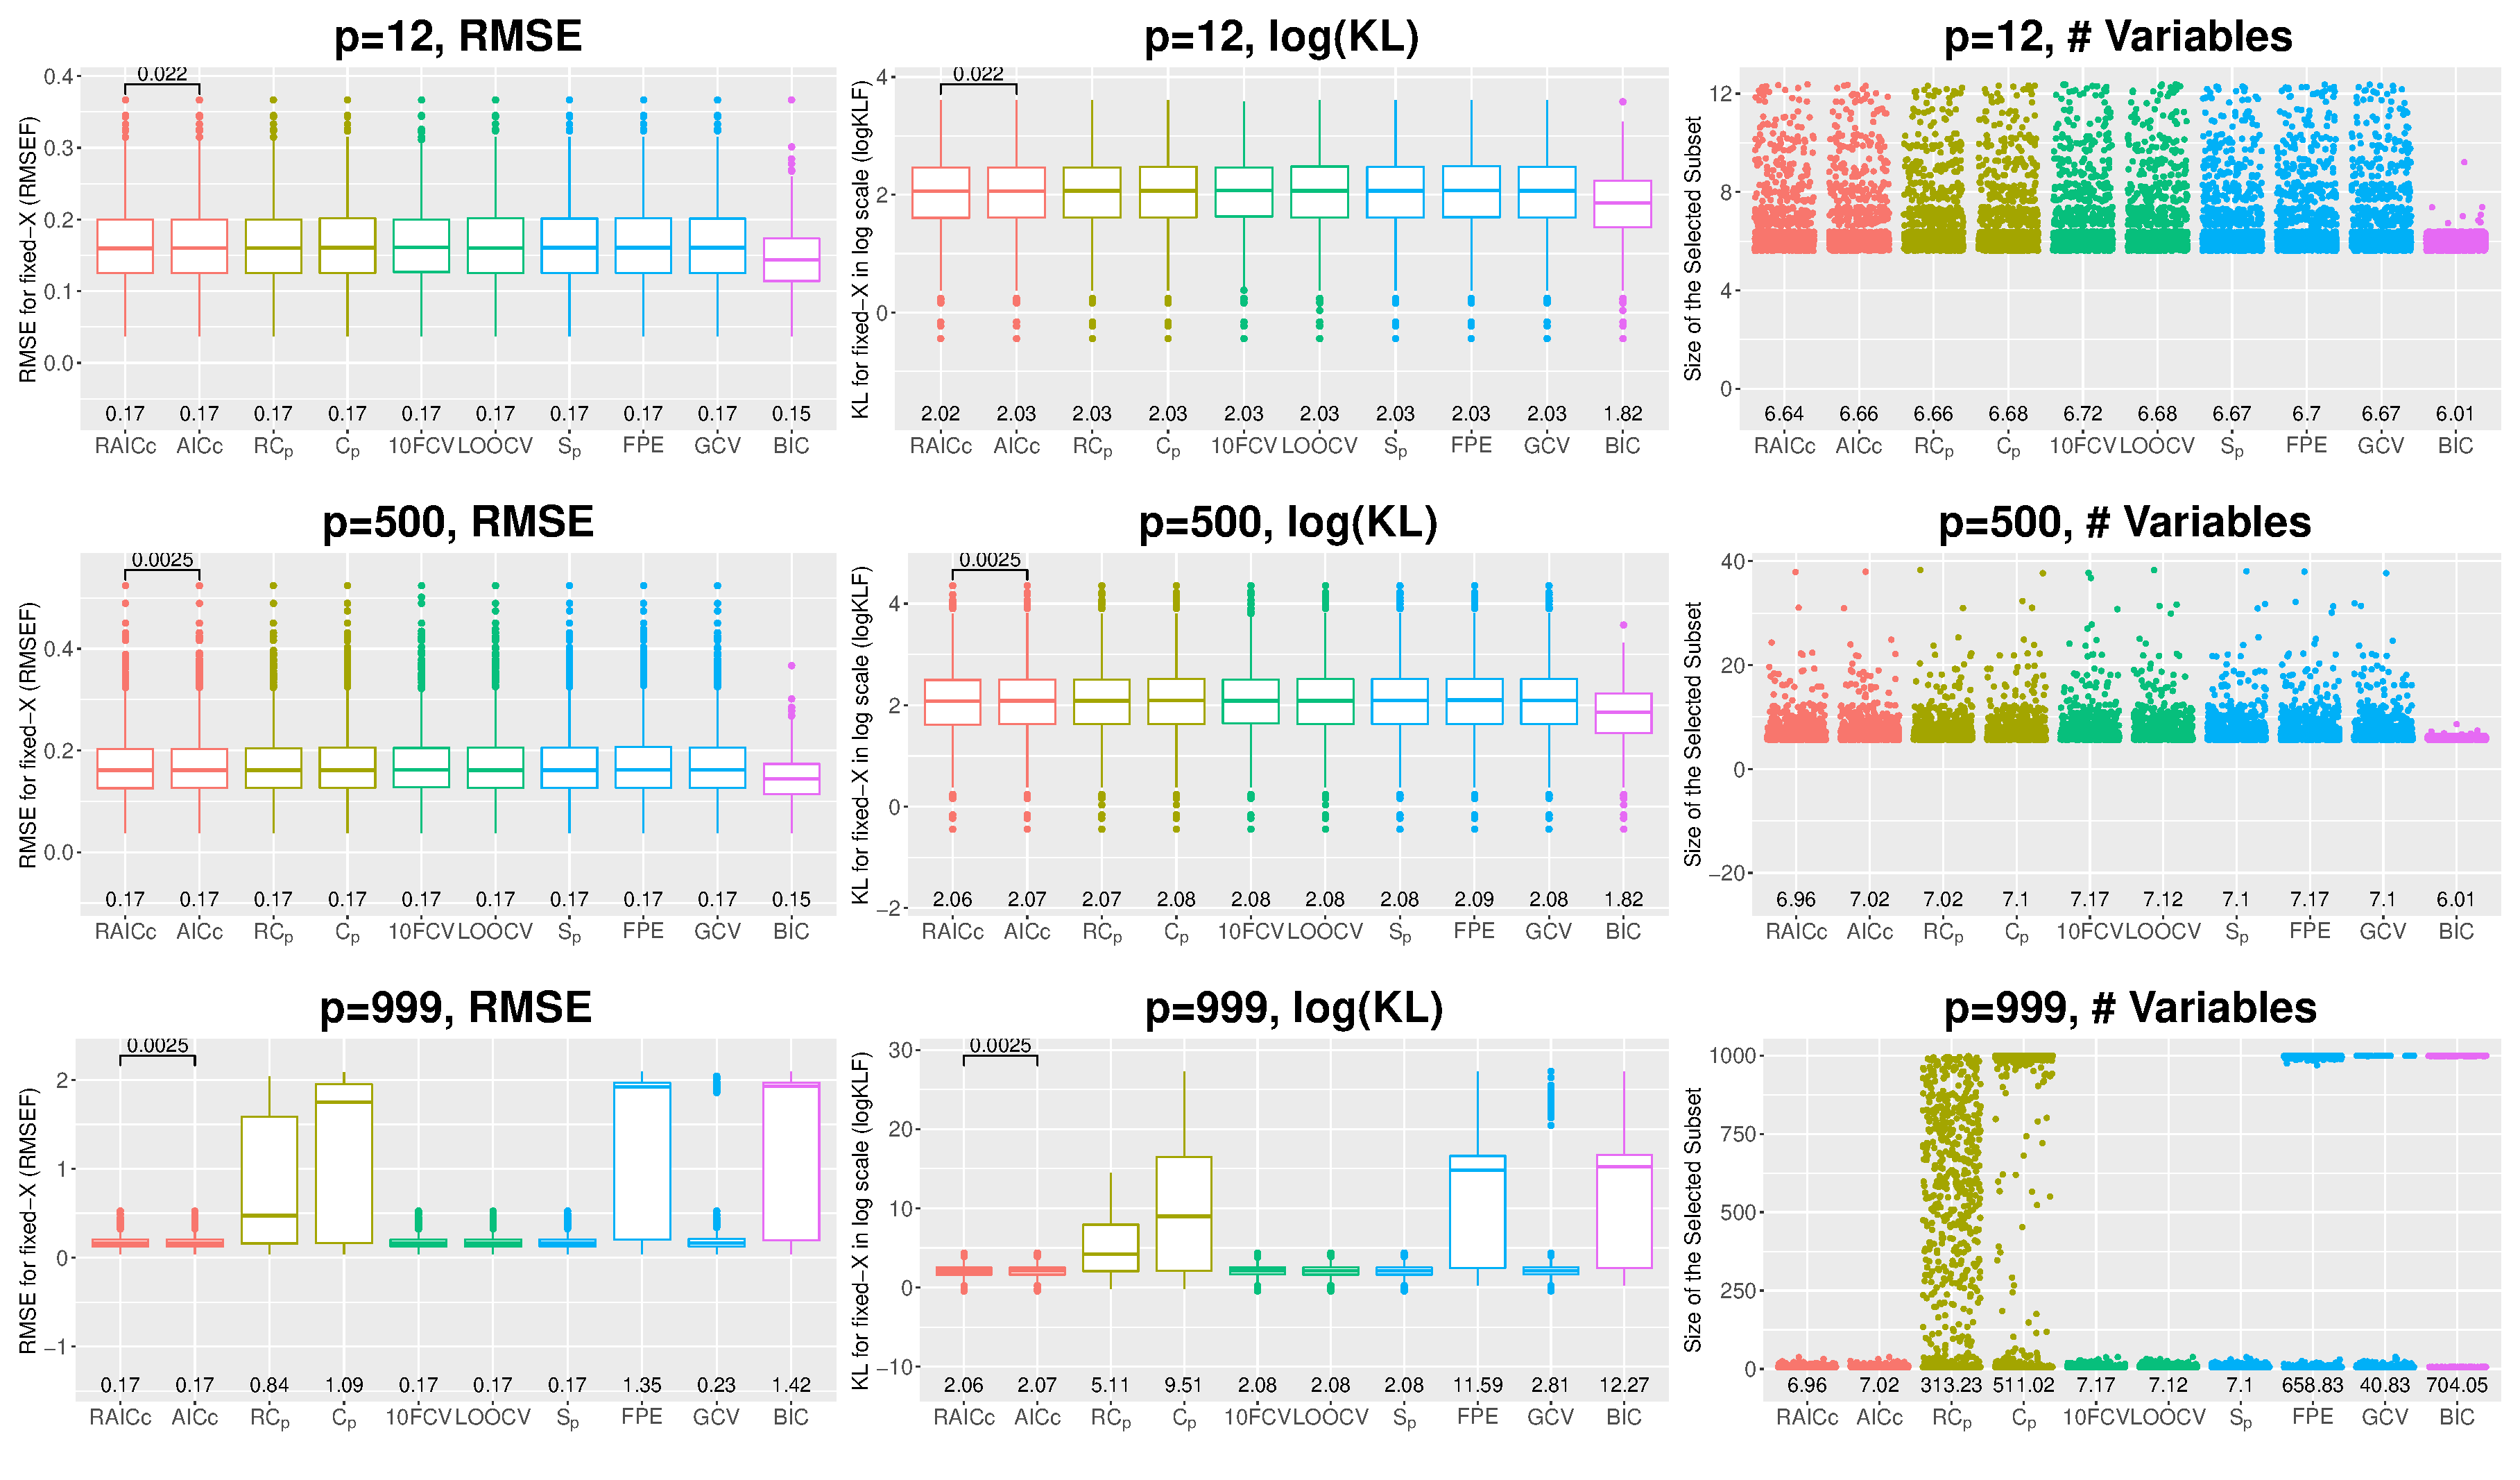
\includegraphics[width=\textwidth]{figures/supplement/fixedx_VS-Ex1_n1000_hsnr_rho0.eps}
\caption{VS-Ex1, $n=1000$, high signal, $\rho=0$, and Fixed-X.}
\end{figure}
\clearpage
\begin{figure}[!ht]
\centering
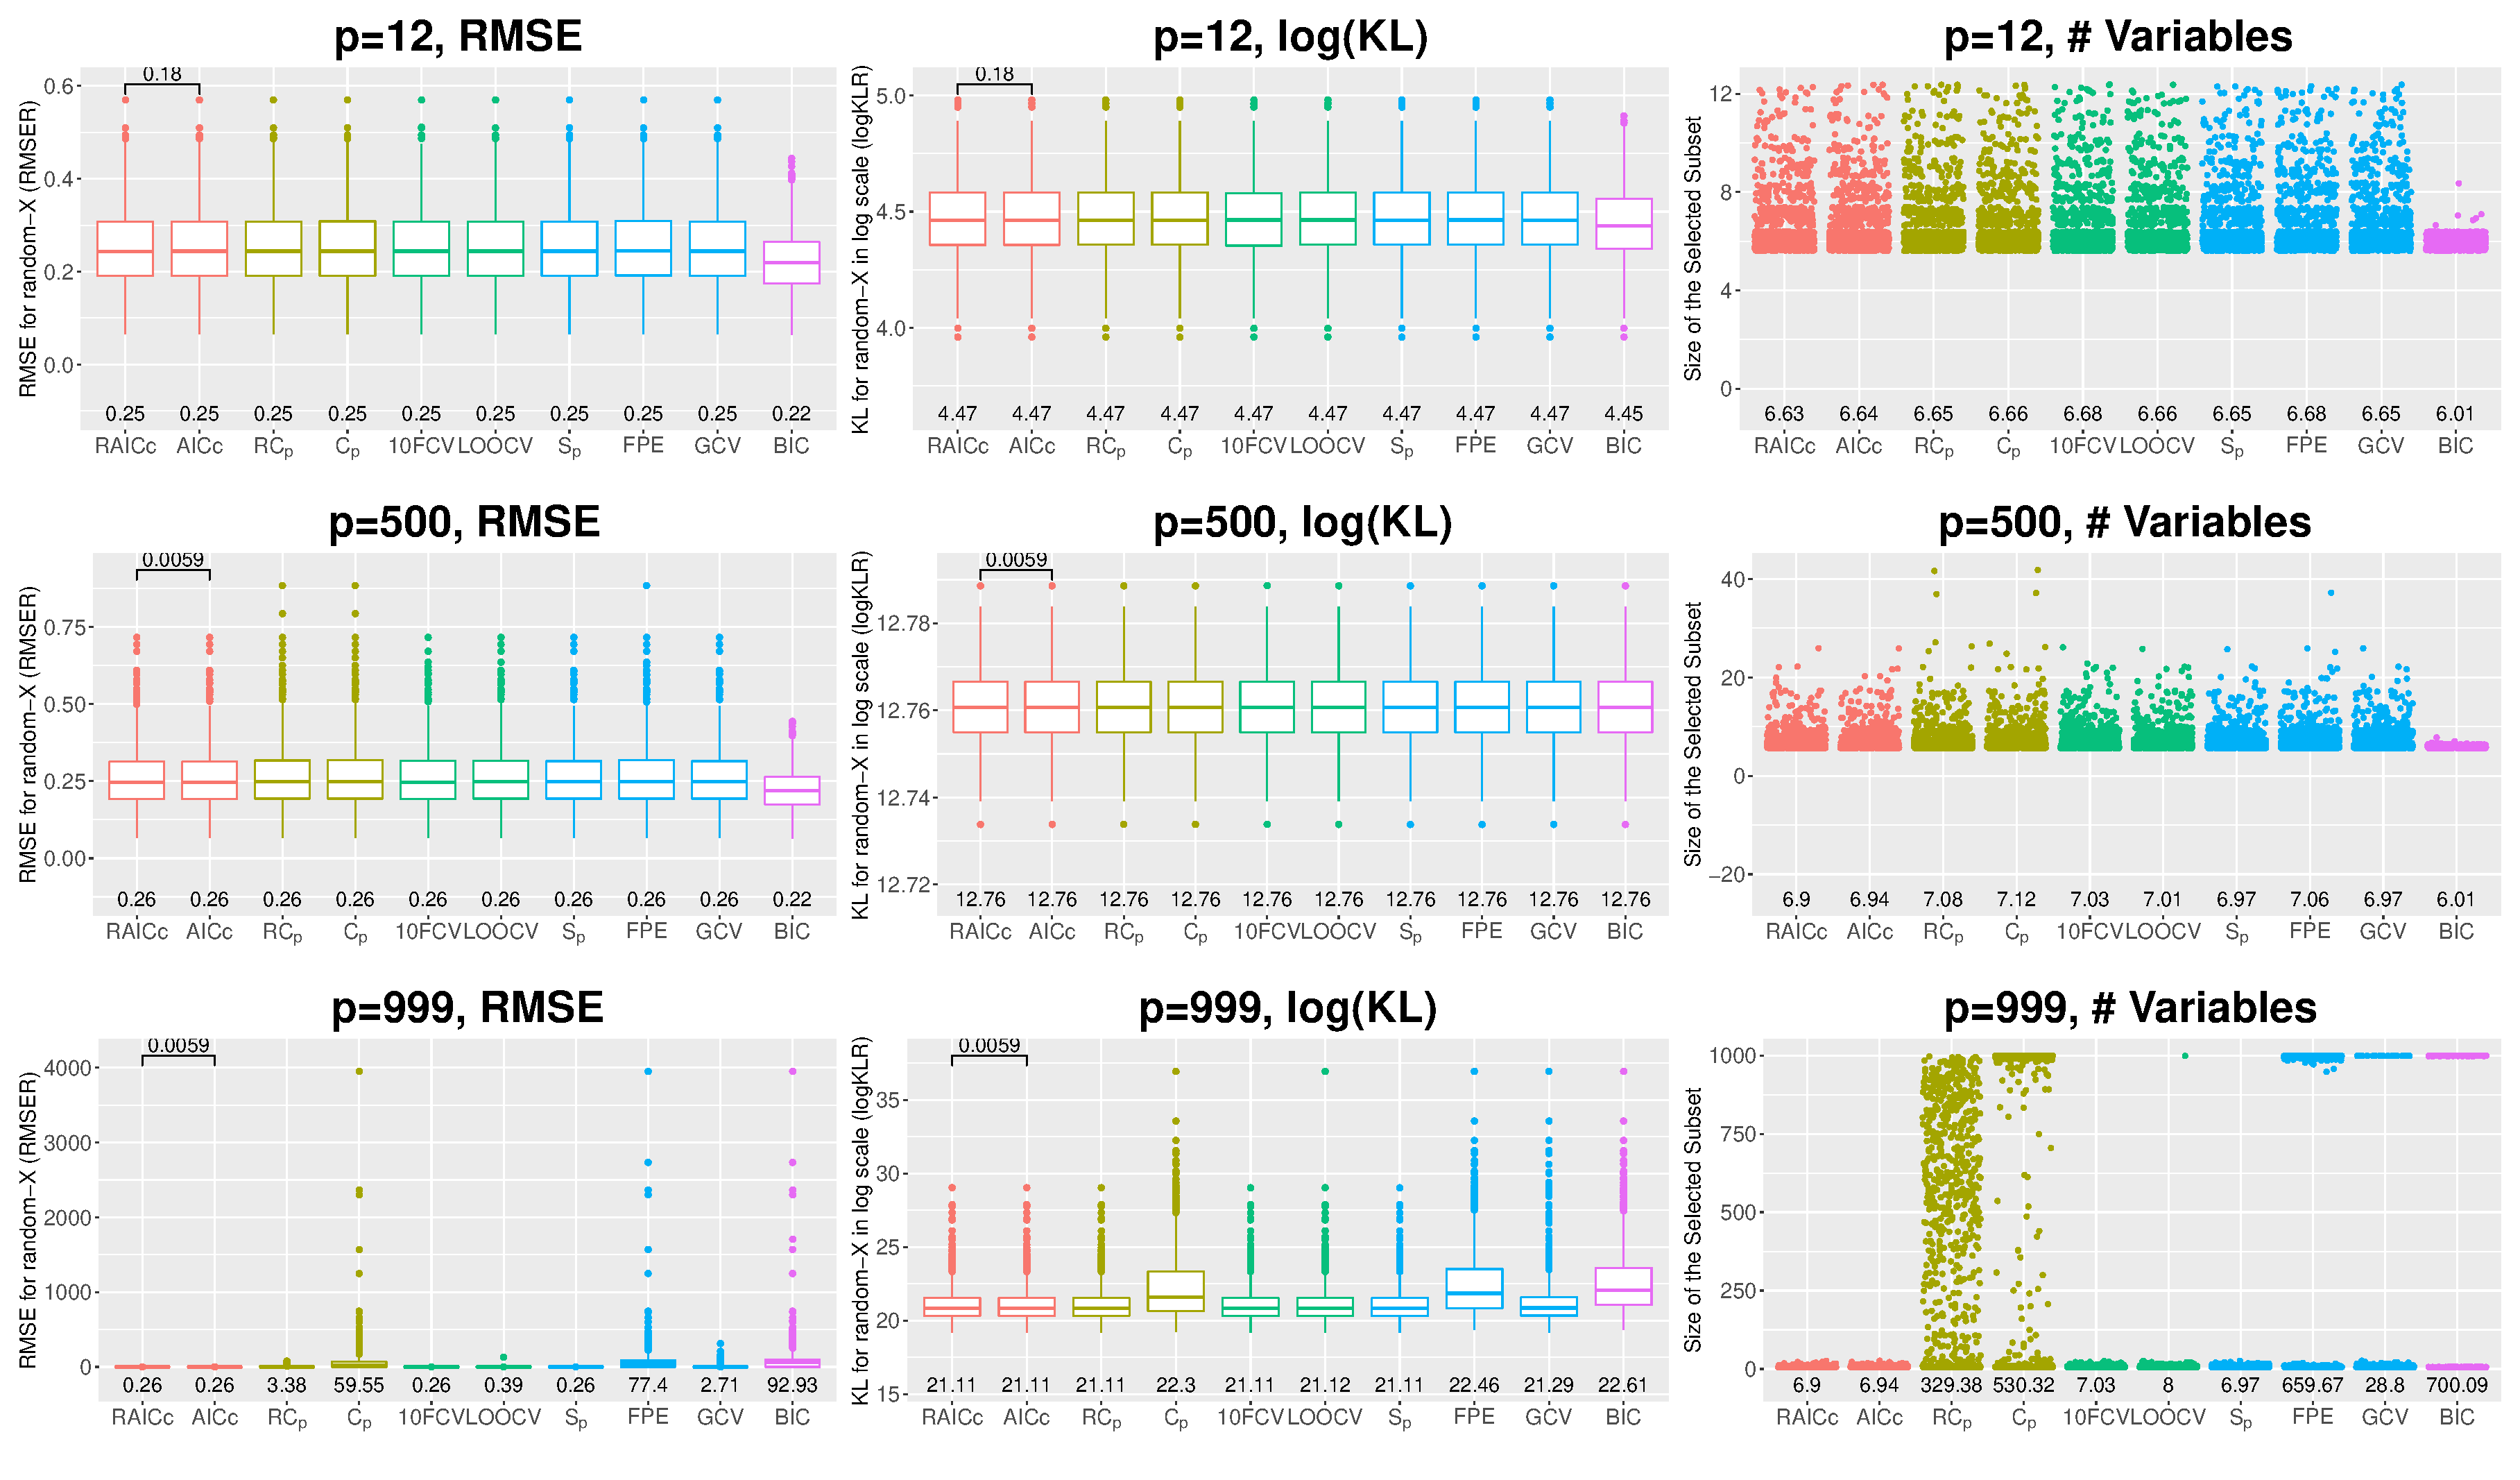
\includegraphics[width=\textwidth]{figures/supplement/randomx_VS-Ex1_n1000_hsnr_rho05.eps}
\caption{VS-Ex1, $n=1000$, high signal, $\rho=0.5$, and Random-X.}
\end{figure}
\begin{figure}[!ht]
\centering
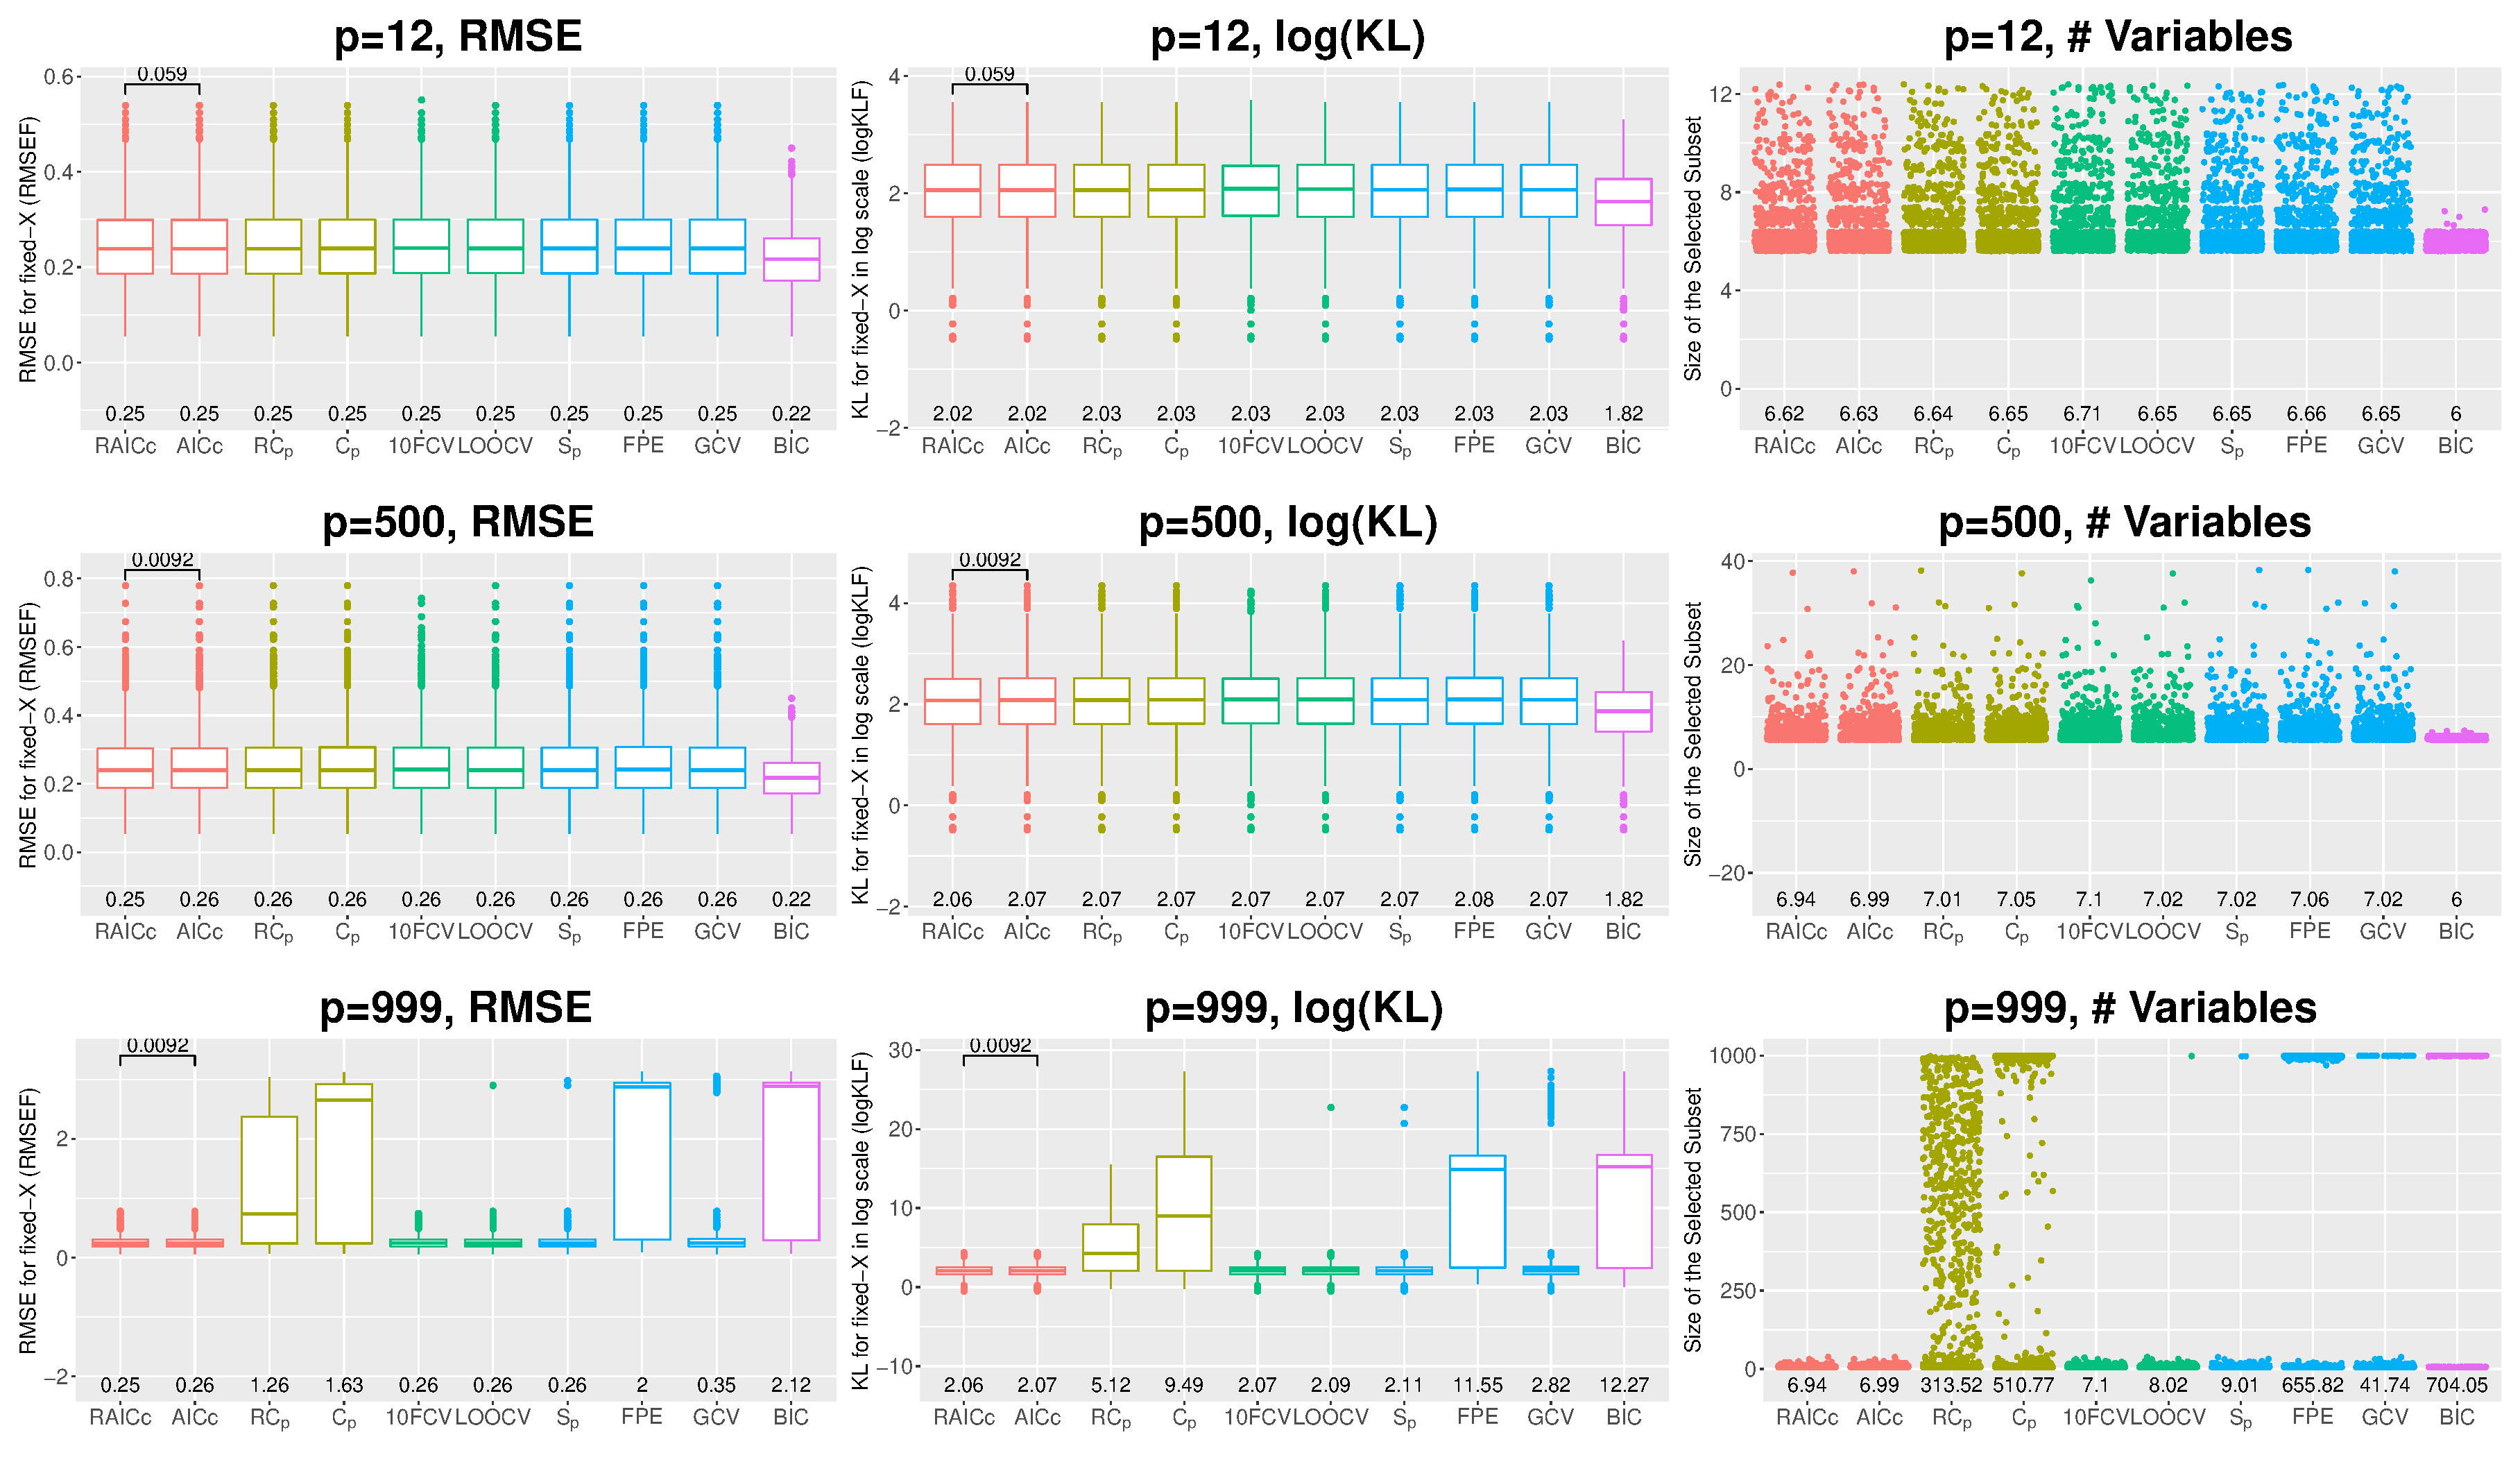
\includegraphics[width=\textwidth]{figures/supplement/fixedx_VS-Ex1_n1000_hsnr_rho05.eps}
\caption{VS-Ex1, $n=1000$, high signal, $\rho=0.5$, and Fixed-X.}
\end{figure}
\clearpage
\begin{figure}[!ht]
\centering
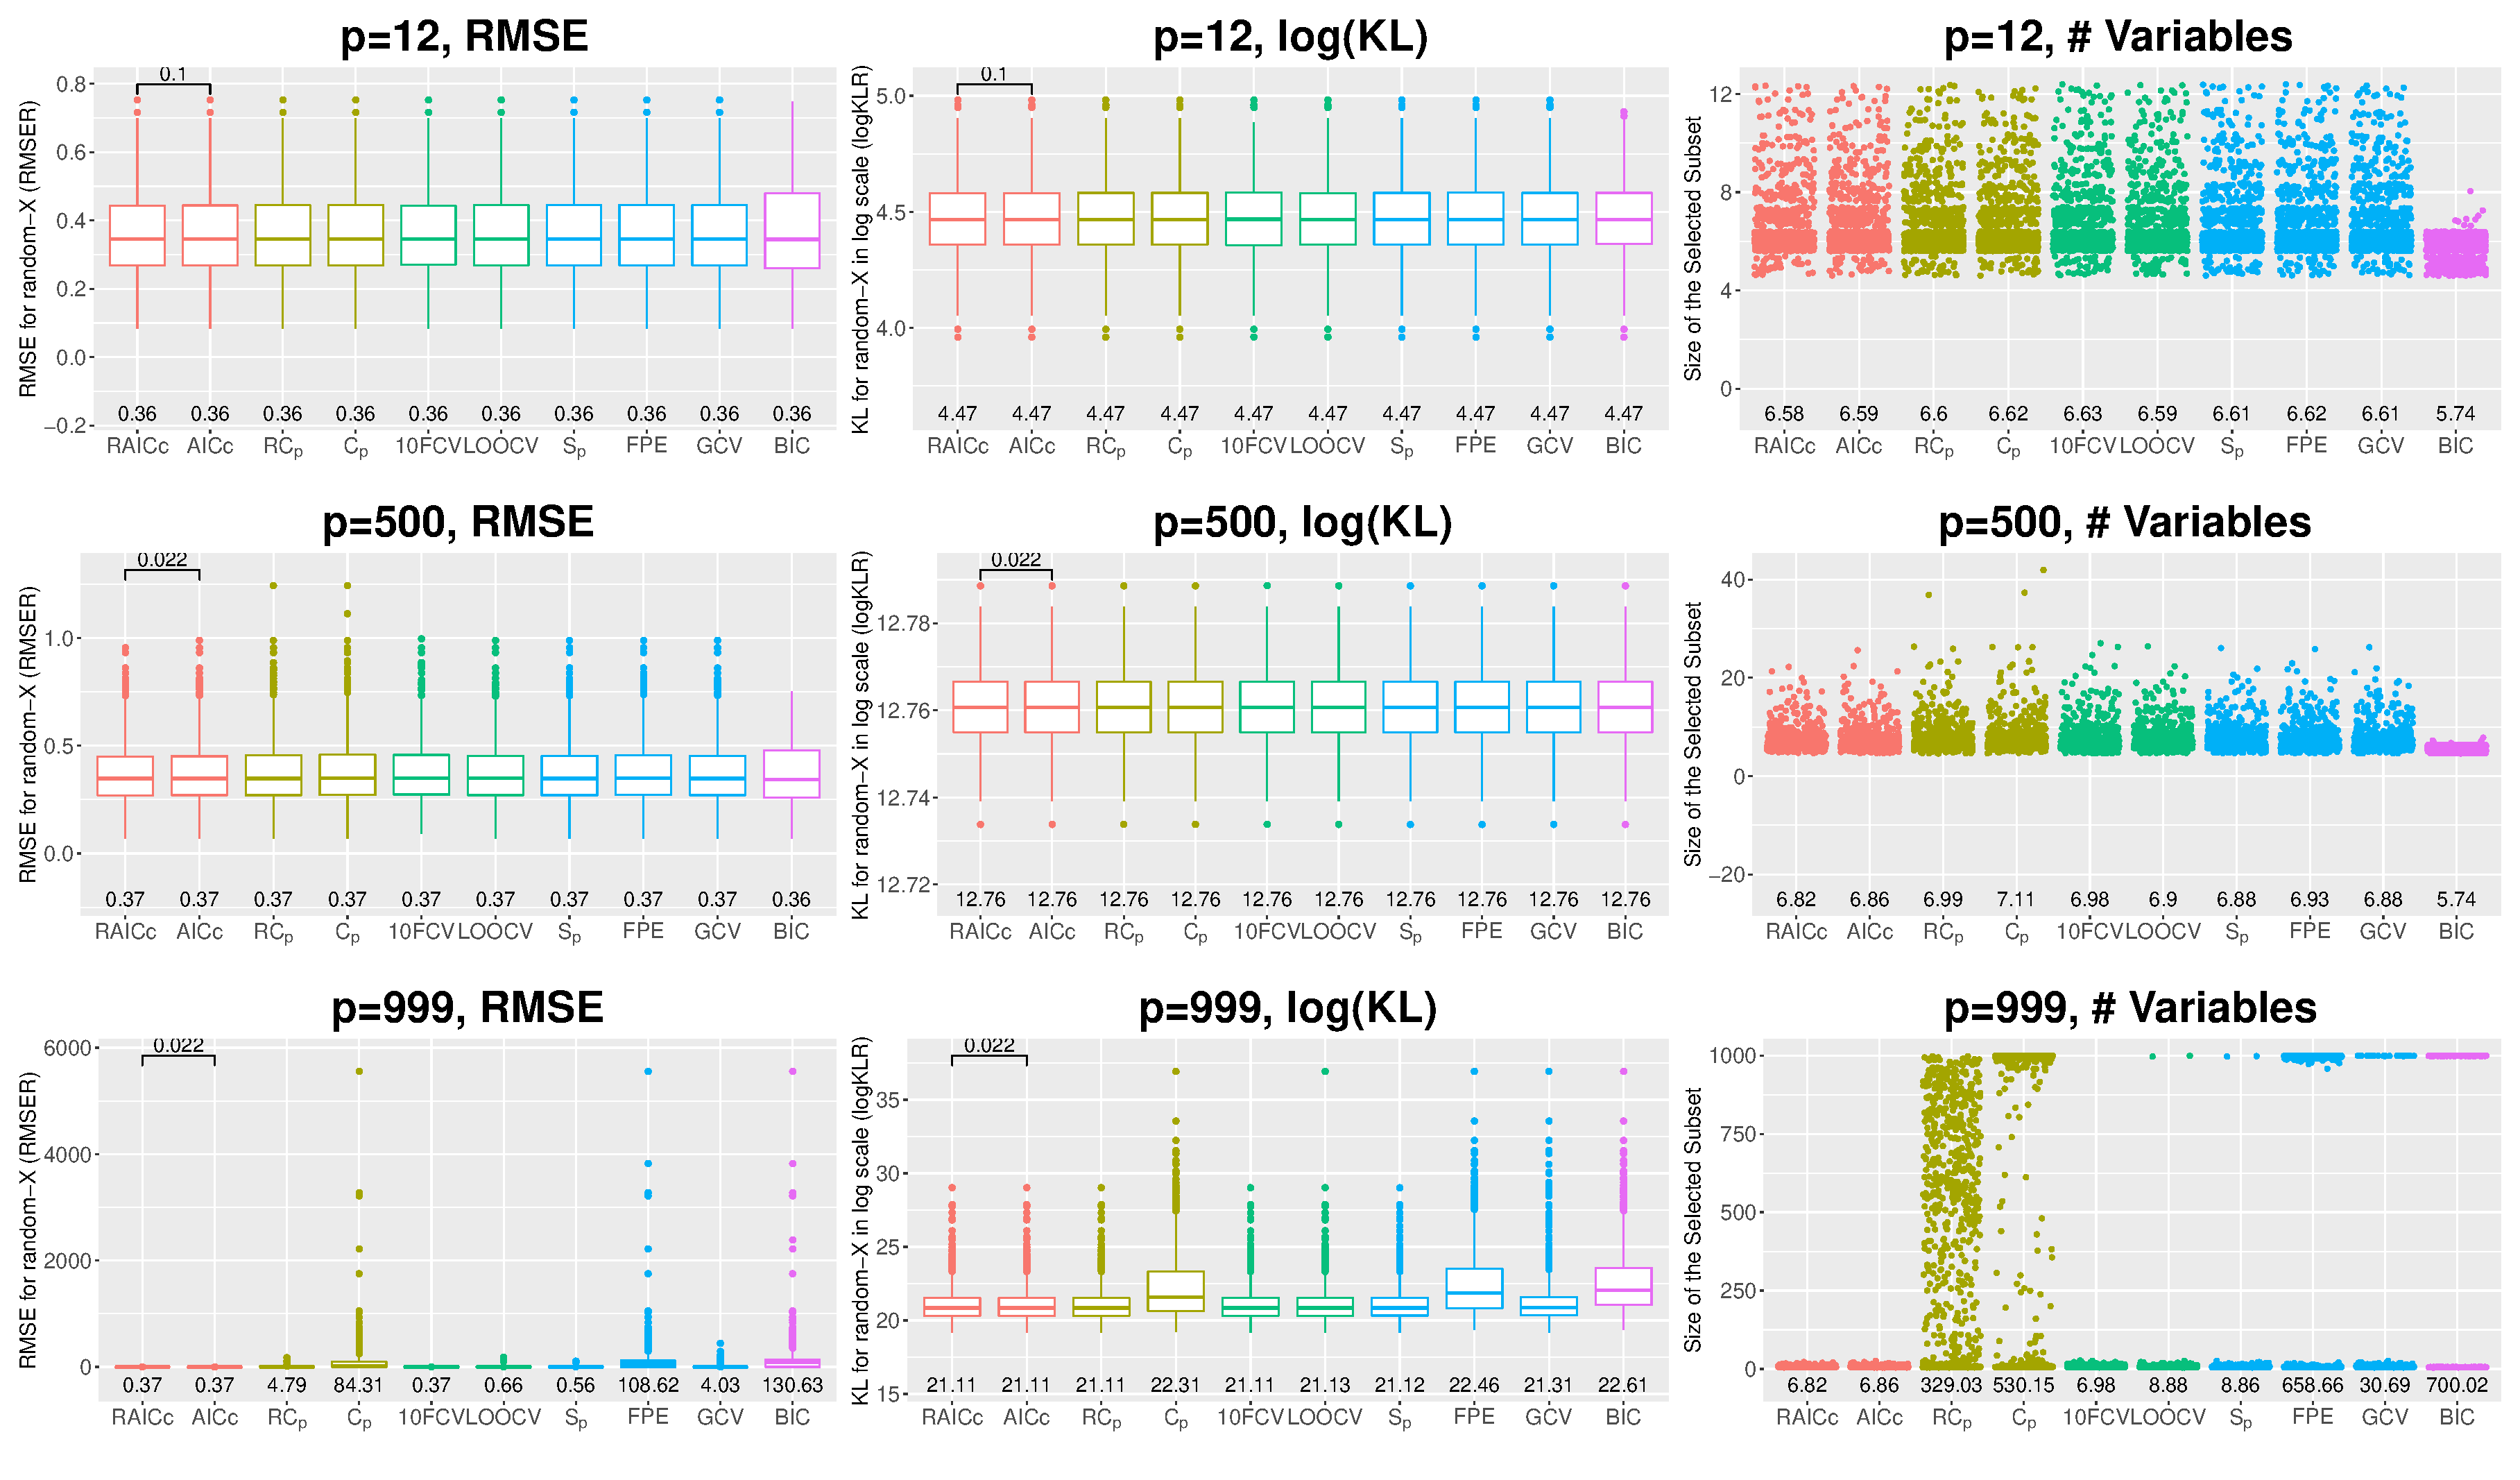
\includegraphics[width=\textwidth]{figures/supplement/randomx_VS-Ex1_n1000_hsnr_rho09.eps}
\caption{VS-Ex1, $n=1000$, high signal, $\rho=0.9$, and Random-X.}
\end{figure}
\begin{figure}[!ht]
\centering
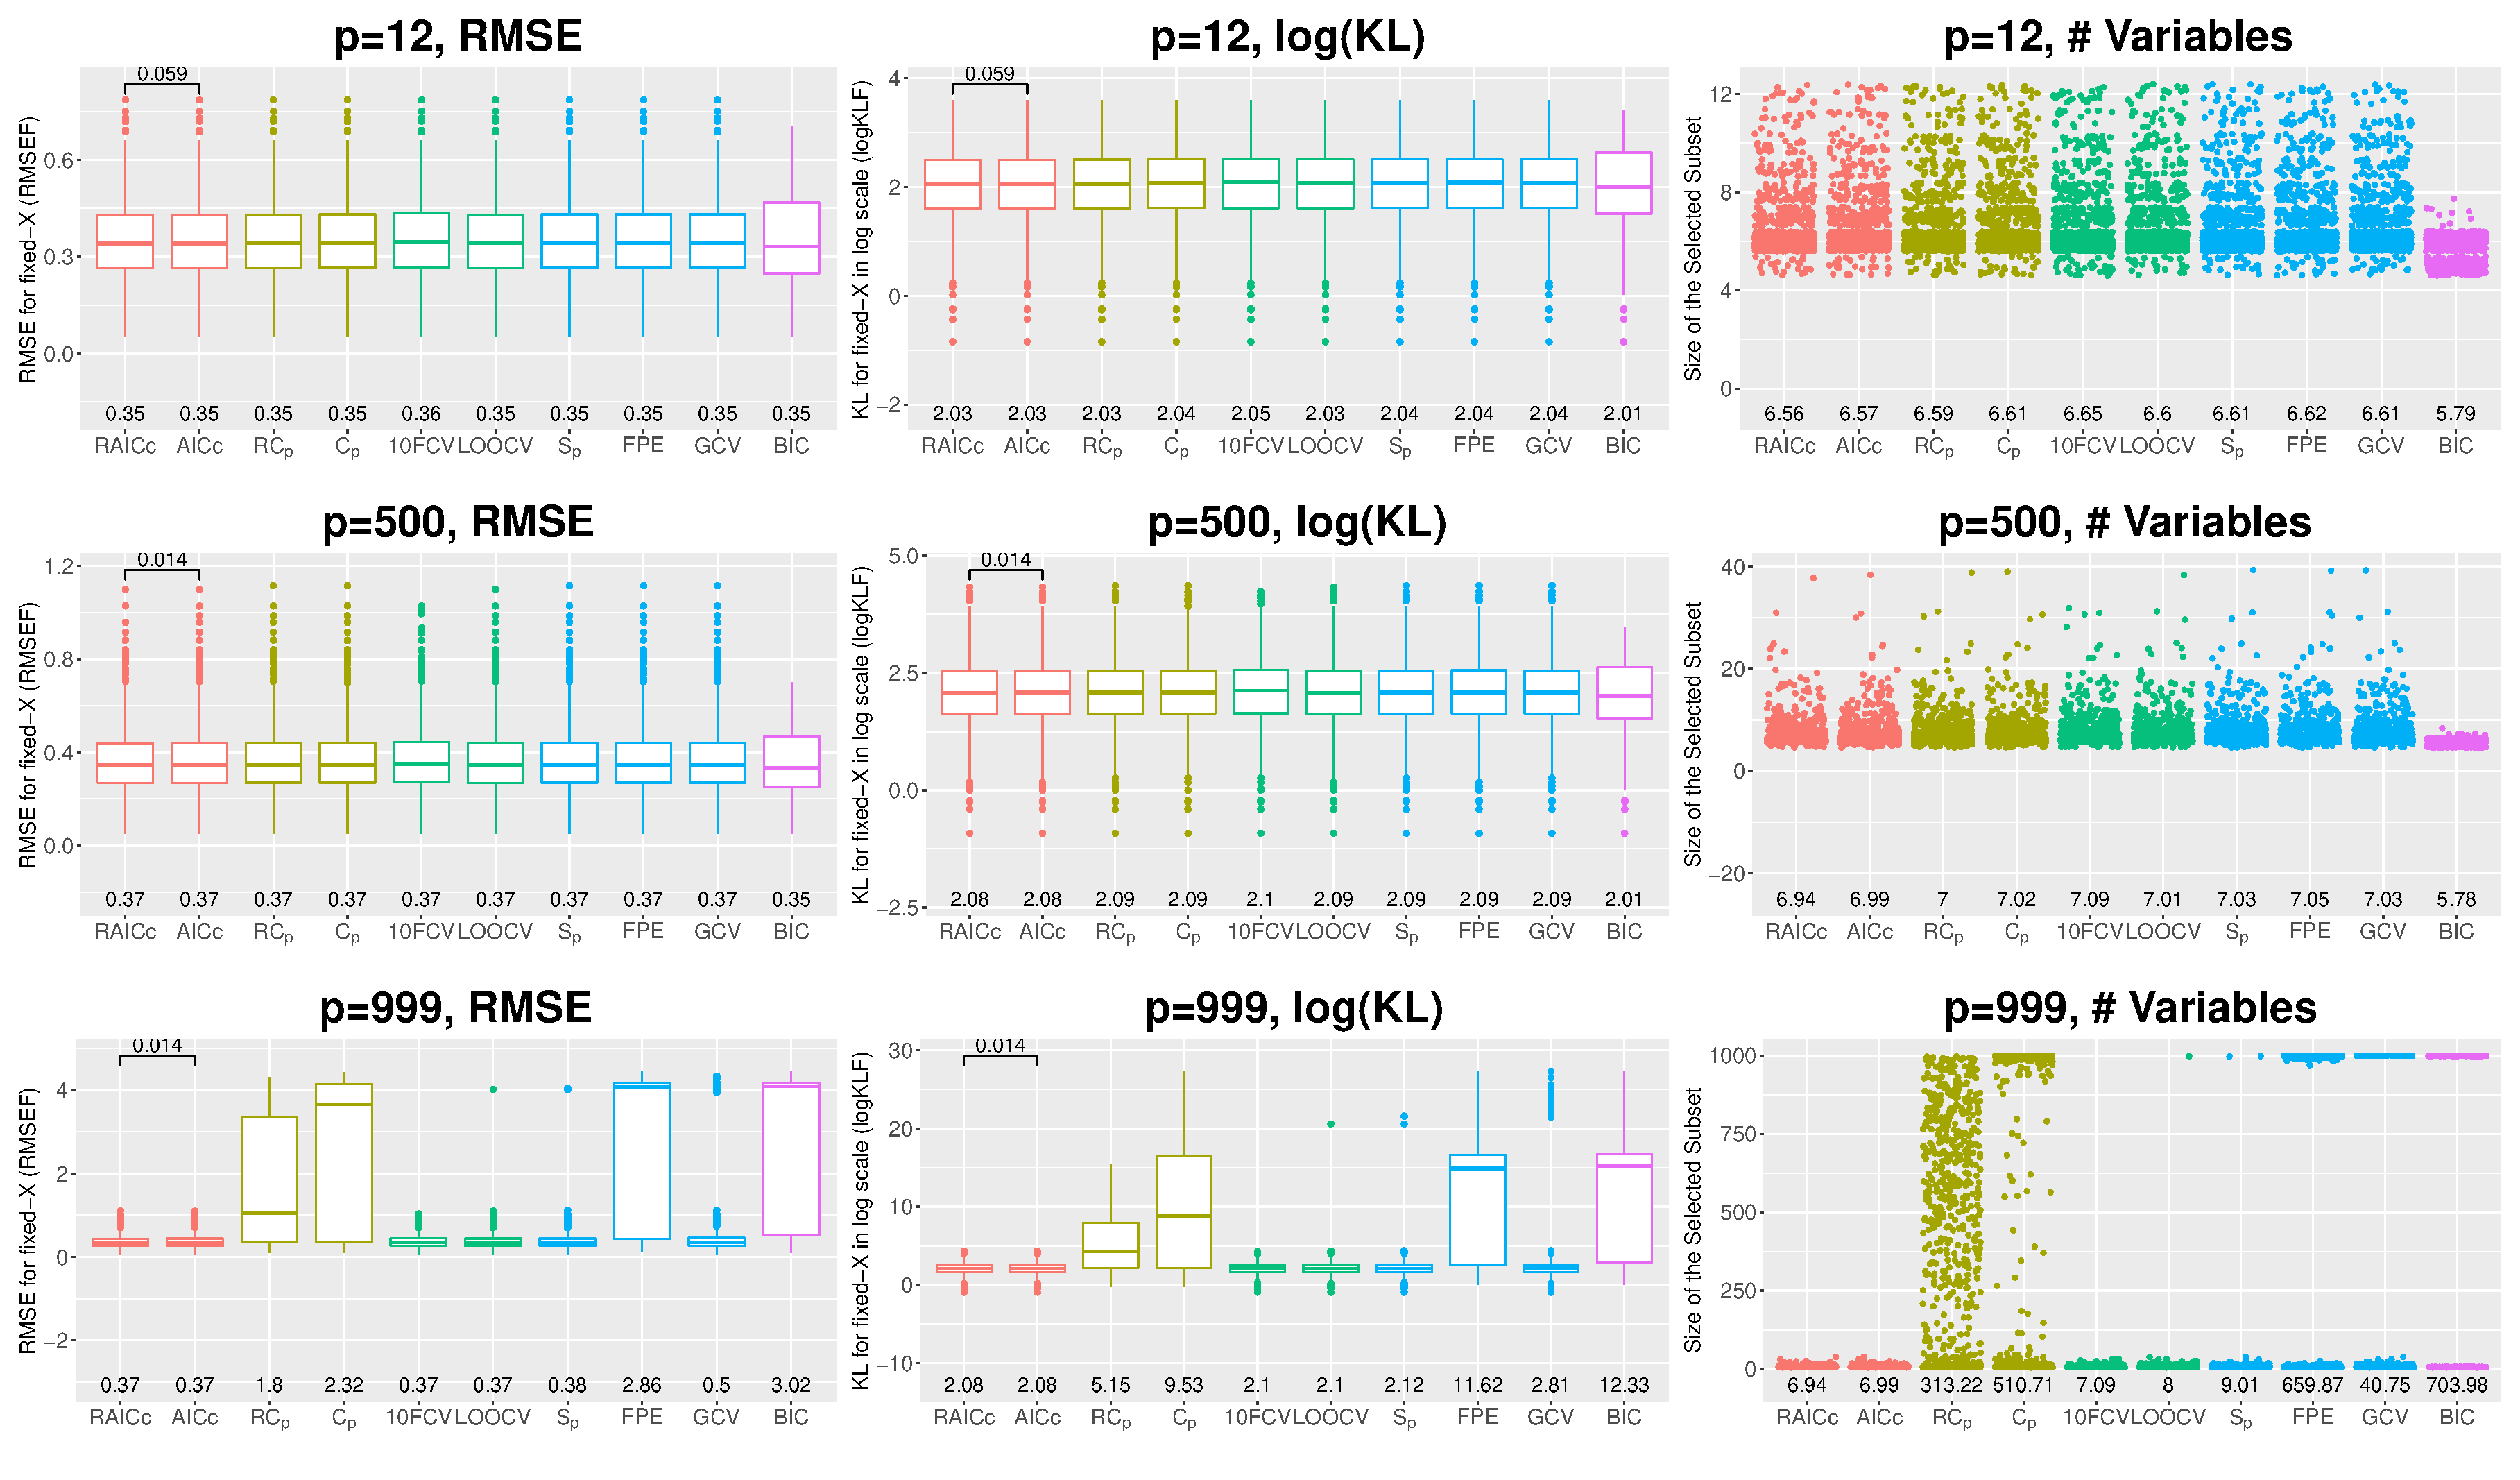
\includegraphics[width=\textwidth]{figures/supplement/fixedx_VS-Ex1_n1000_hsnr_rho09.eps}
\caption{VS-Ex1, $n=1000$, high signal, $\rho=0.9$, and Fixed-X.}
\end{figure}
\clearpage
\begin{figure}[!ht]
\centering
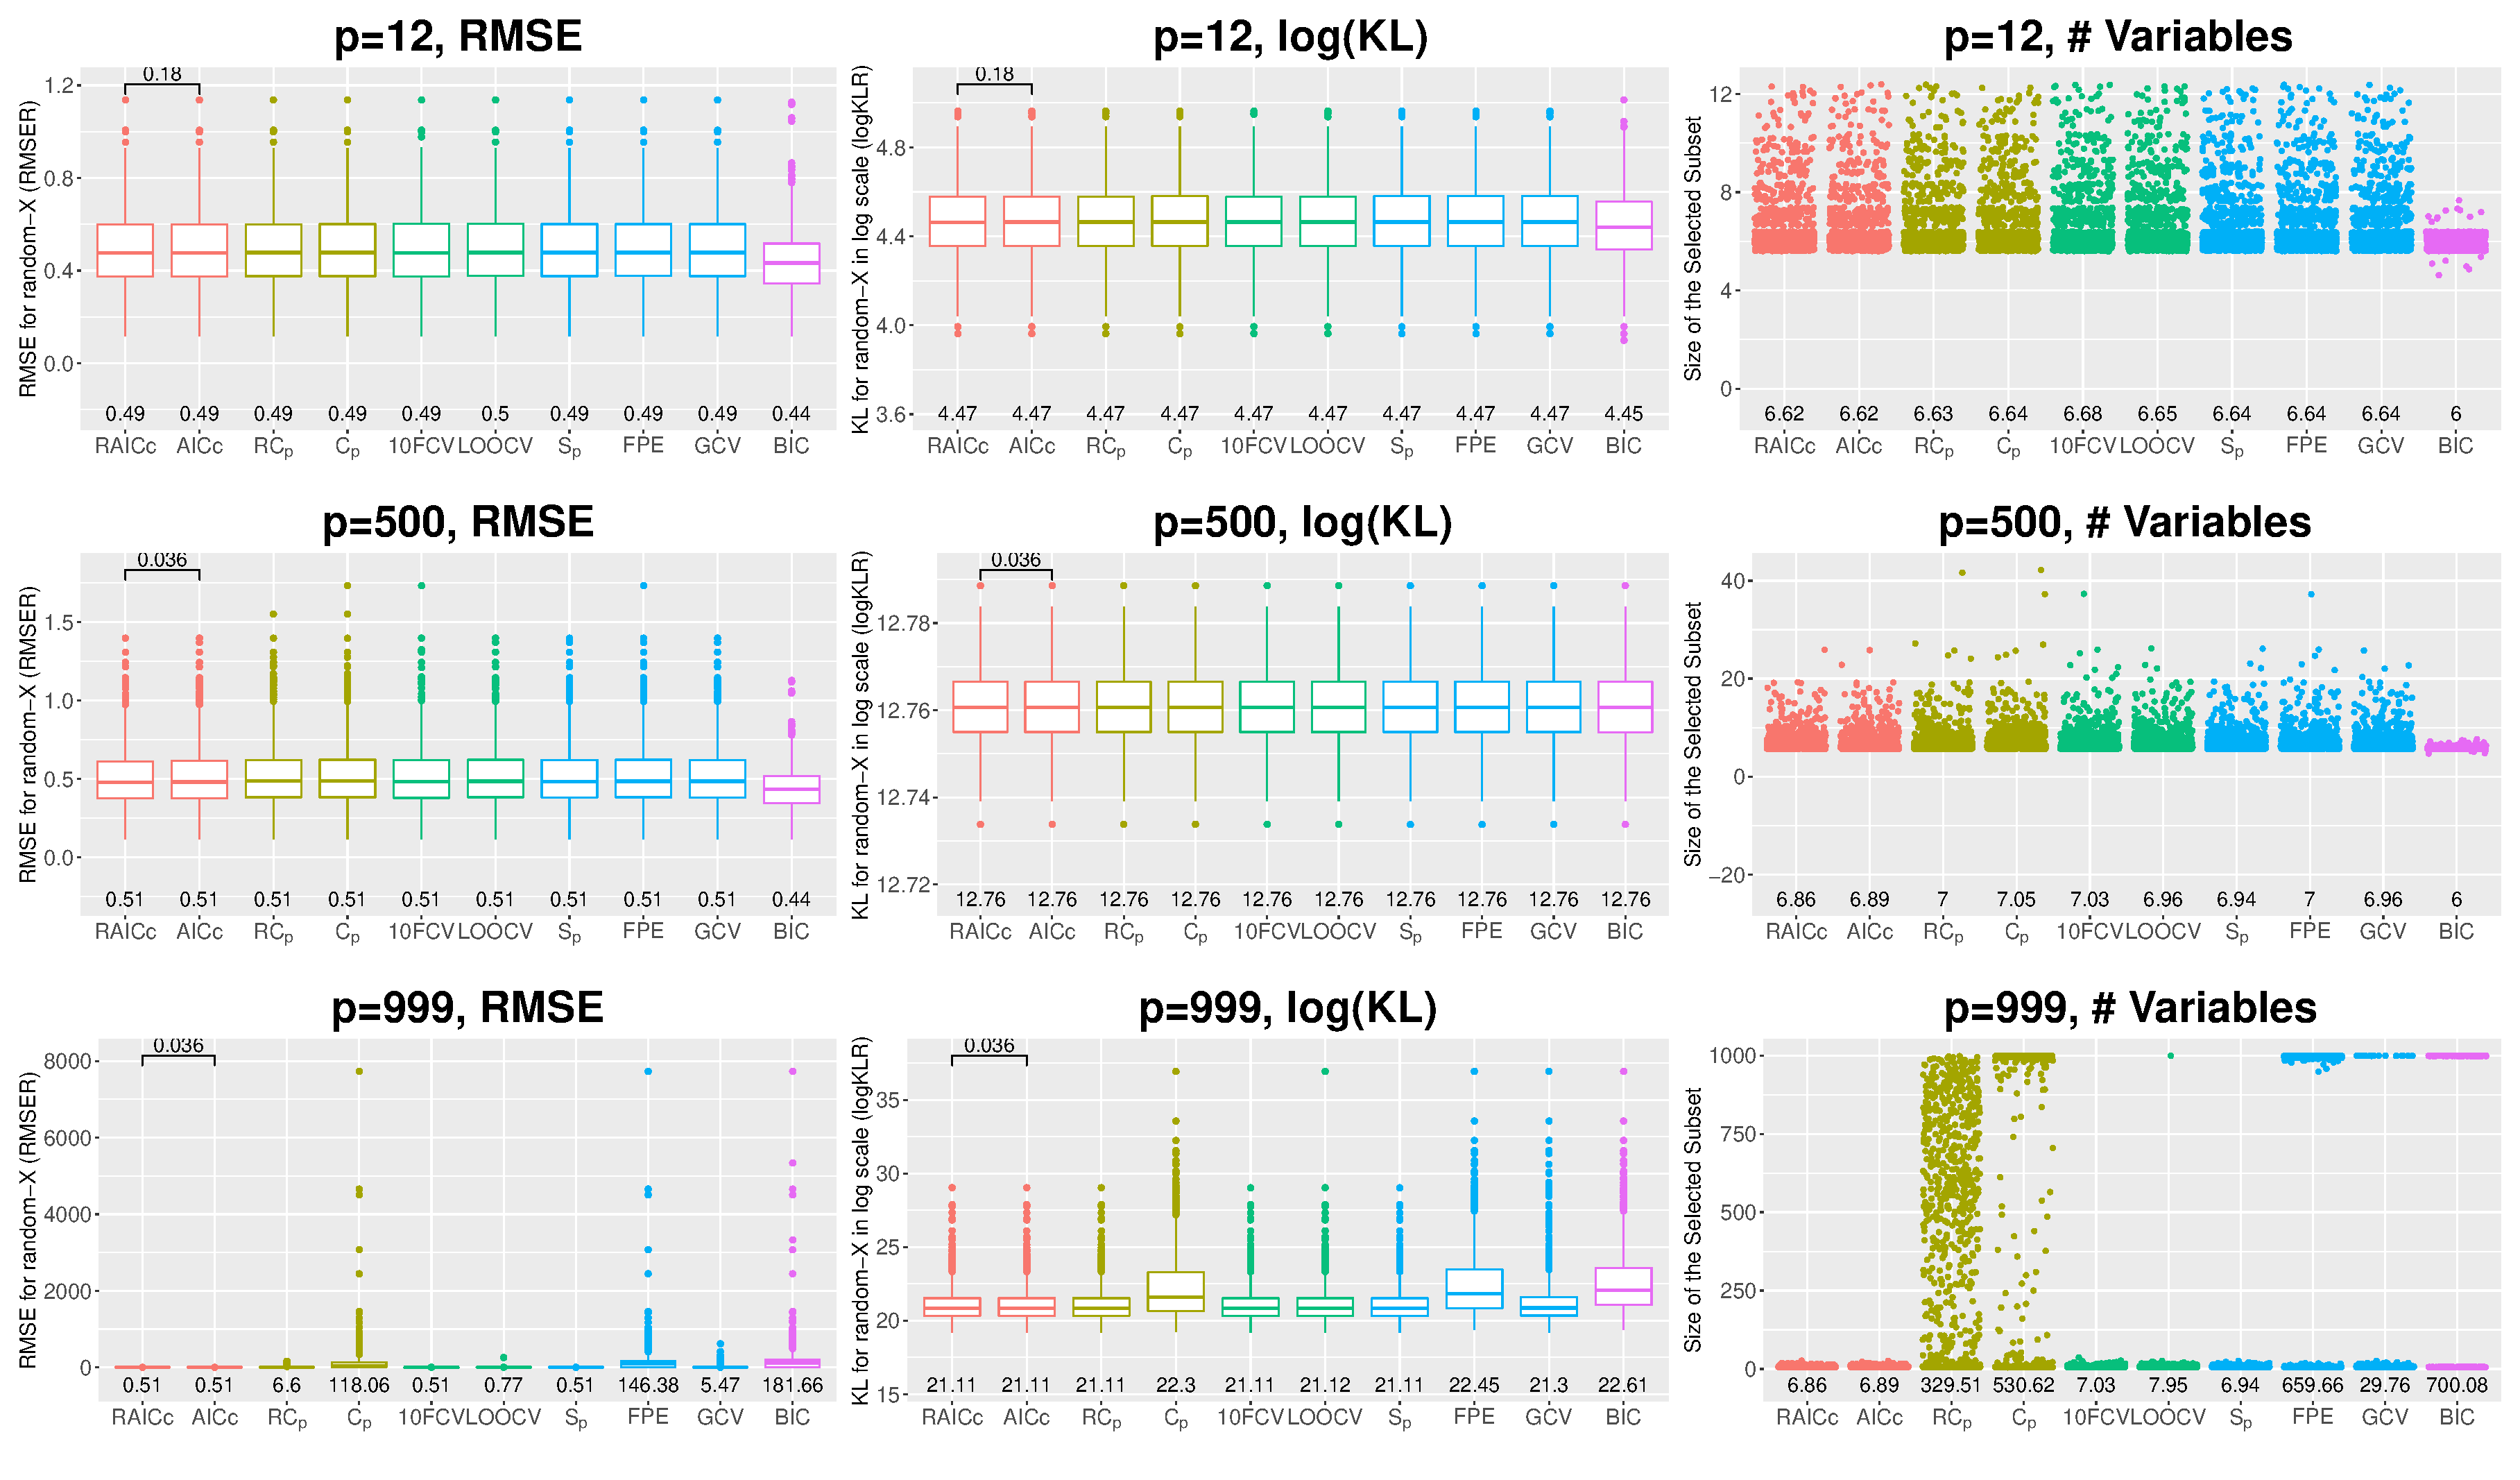
\includegraphics[width=\textwidth]{figures/supplement/randomx_VS-Ex1_n1000_msnr_rho0.eps}
\caption{VS-Ex1, $n=1000$, medium signal, $\rho=0$, and Random-X.}
\end{figure}
\begin{figure}[!ht]
\centering
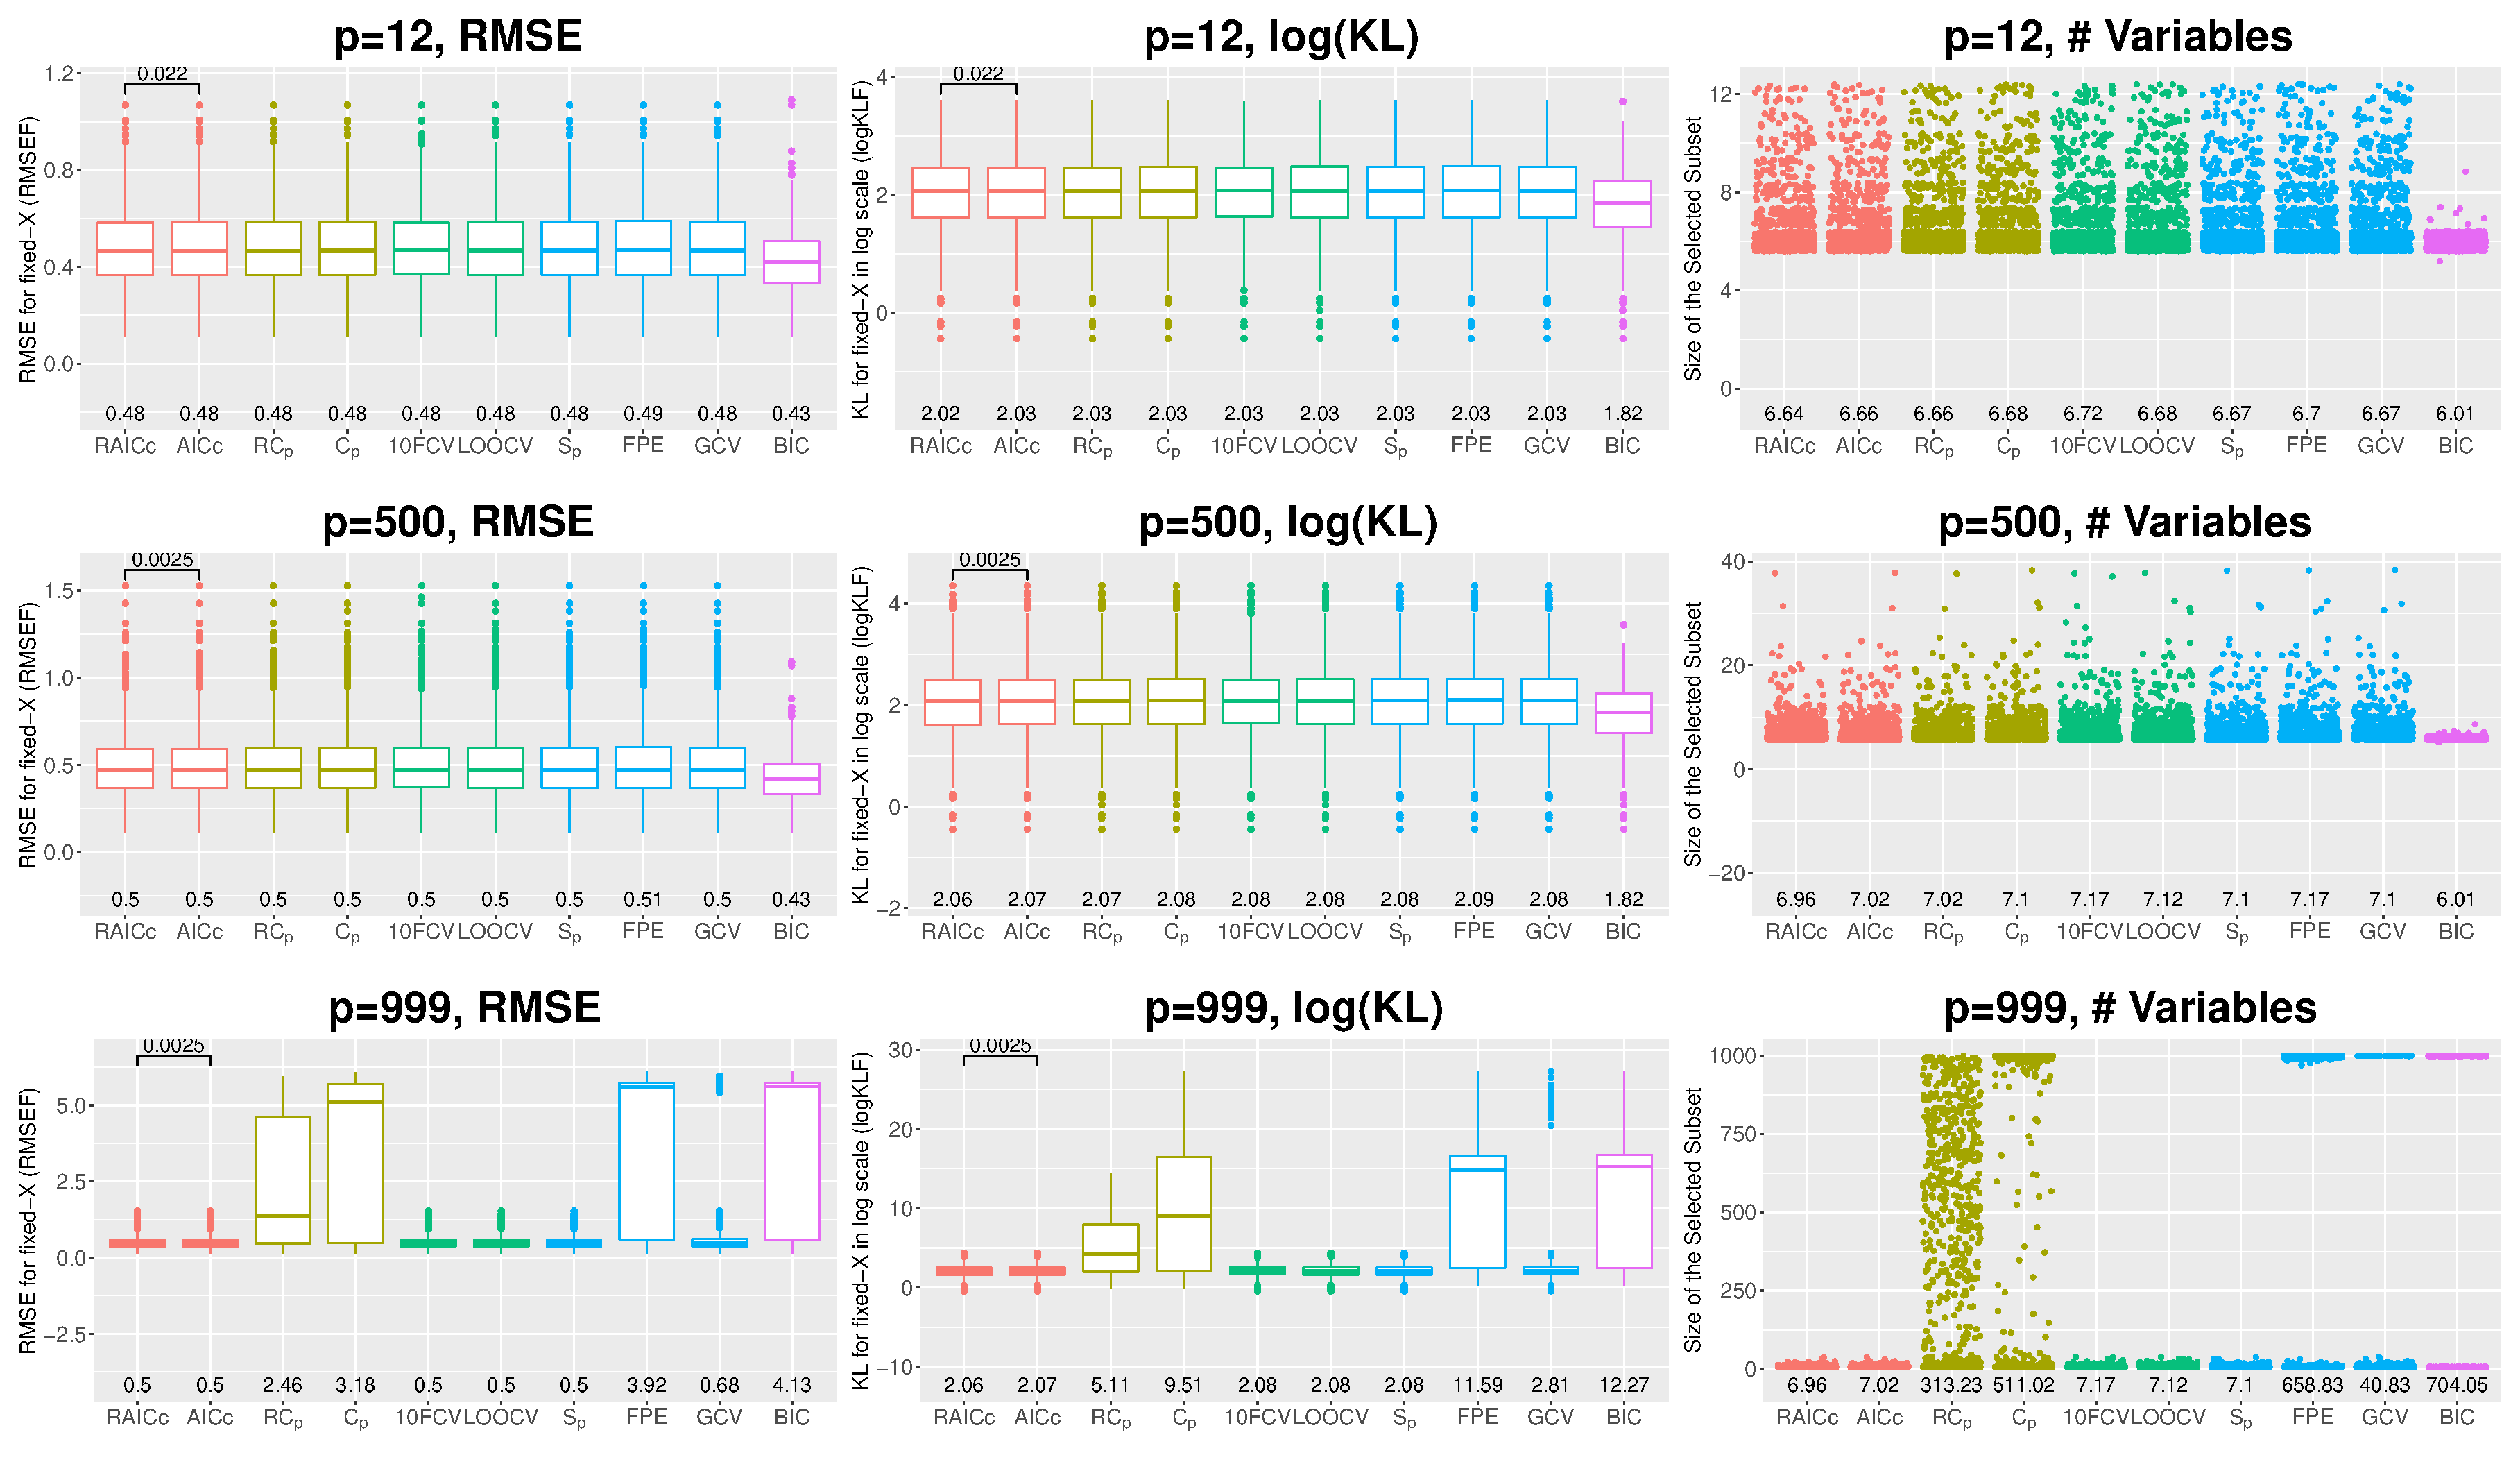
\includegraphics[width=\textwidth]{figures/supplement/fixedx_VS-Ex1_n1000_msnr_rho0.eps}
\caption{VS-Ex1, $n=1000$, medium signal, $\rho=0$, and Fixed-X.}
\end{figure}
\clearpage
\begin{figure}[!ht]
\centering
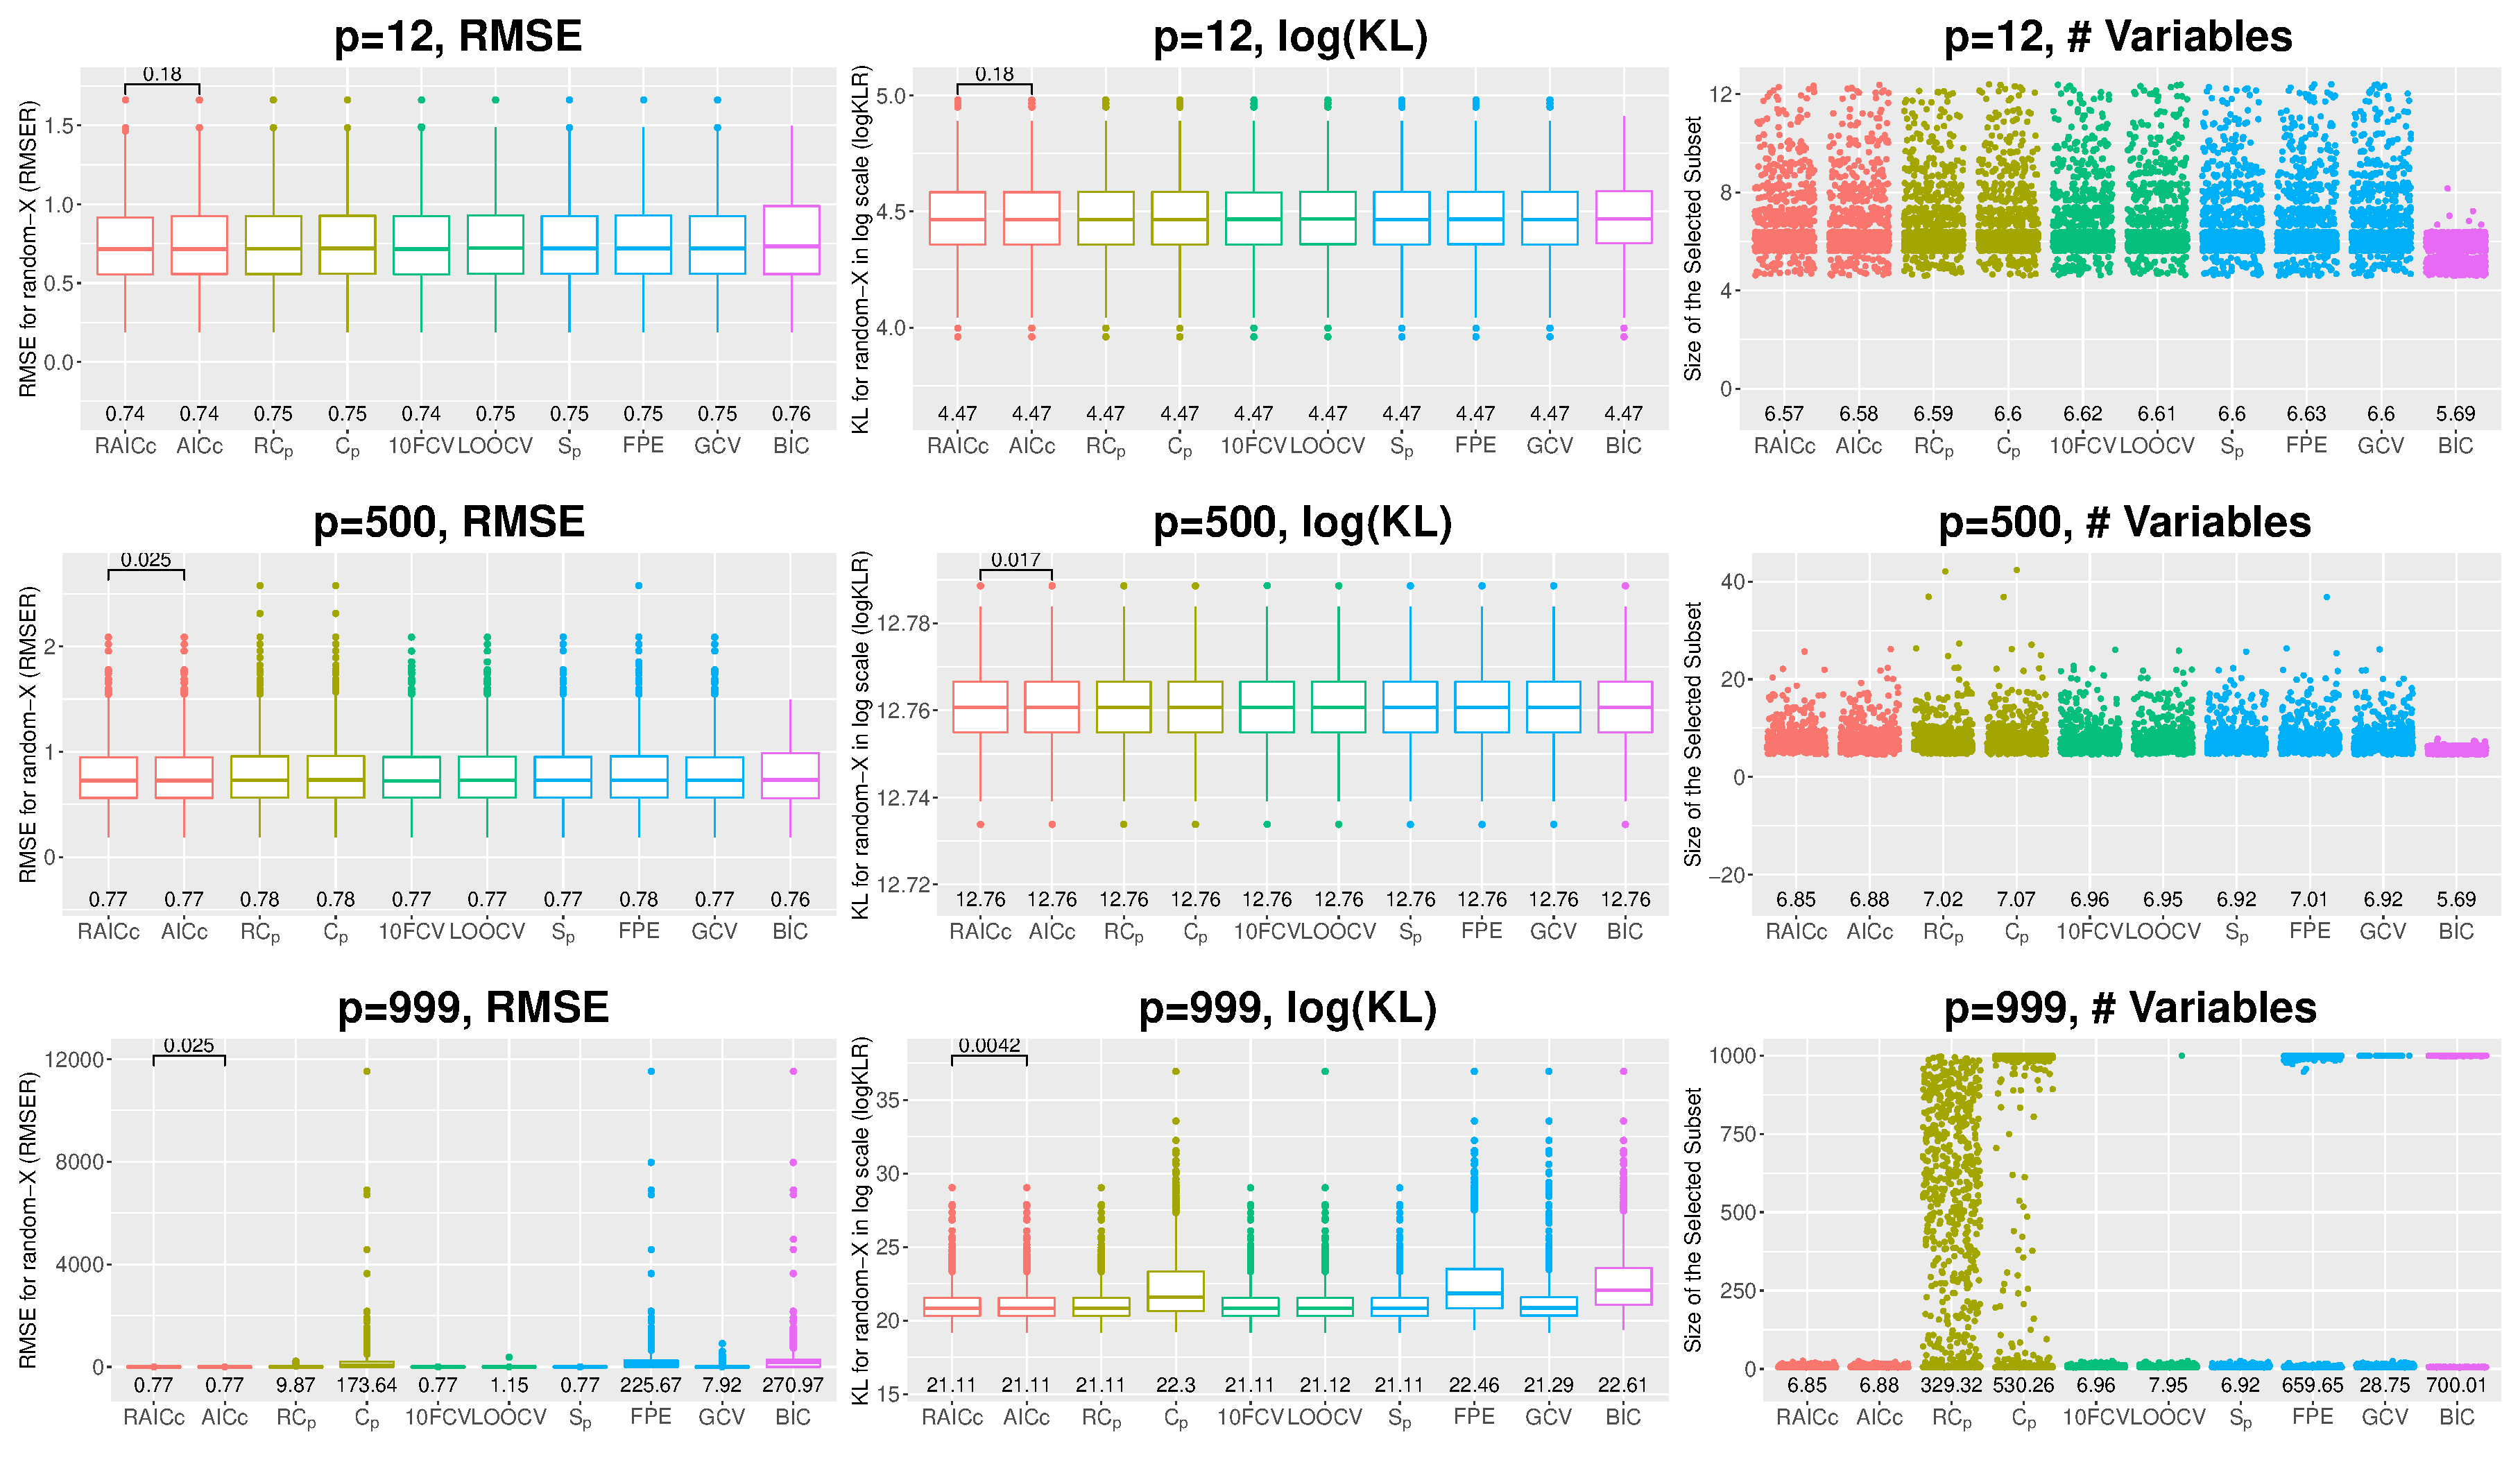
\includegraphics[width=\textwidth]{figures/supplement/randomx_VS-Ex1_n1000_msnr_rho05.eps}
\caption{VS-Ex1, $n=1000$, medium signal, $\rho=0.5$, and Random-X.}
\end{figure}
\begin{figure}[!ht]
\centering
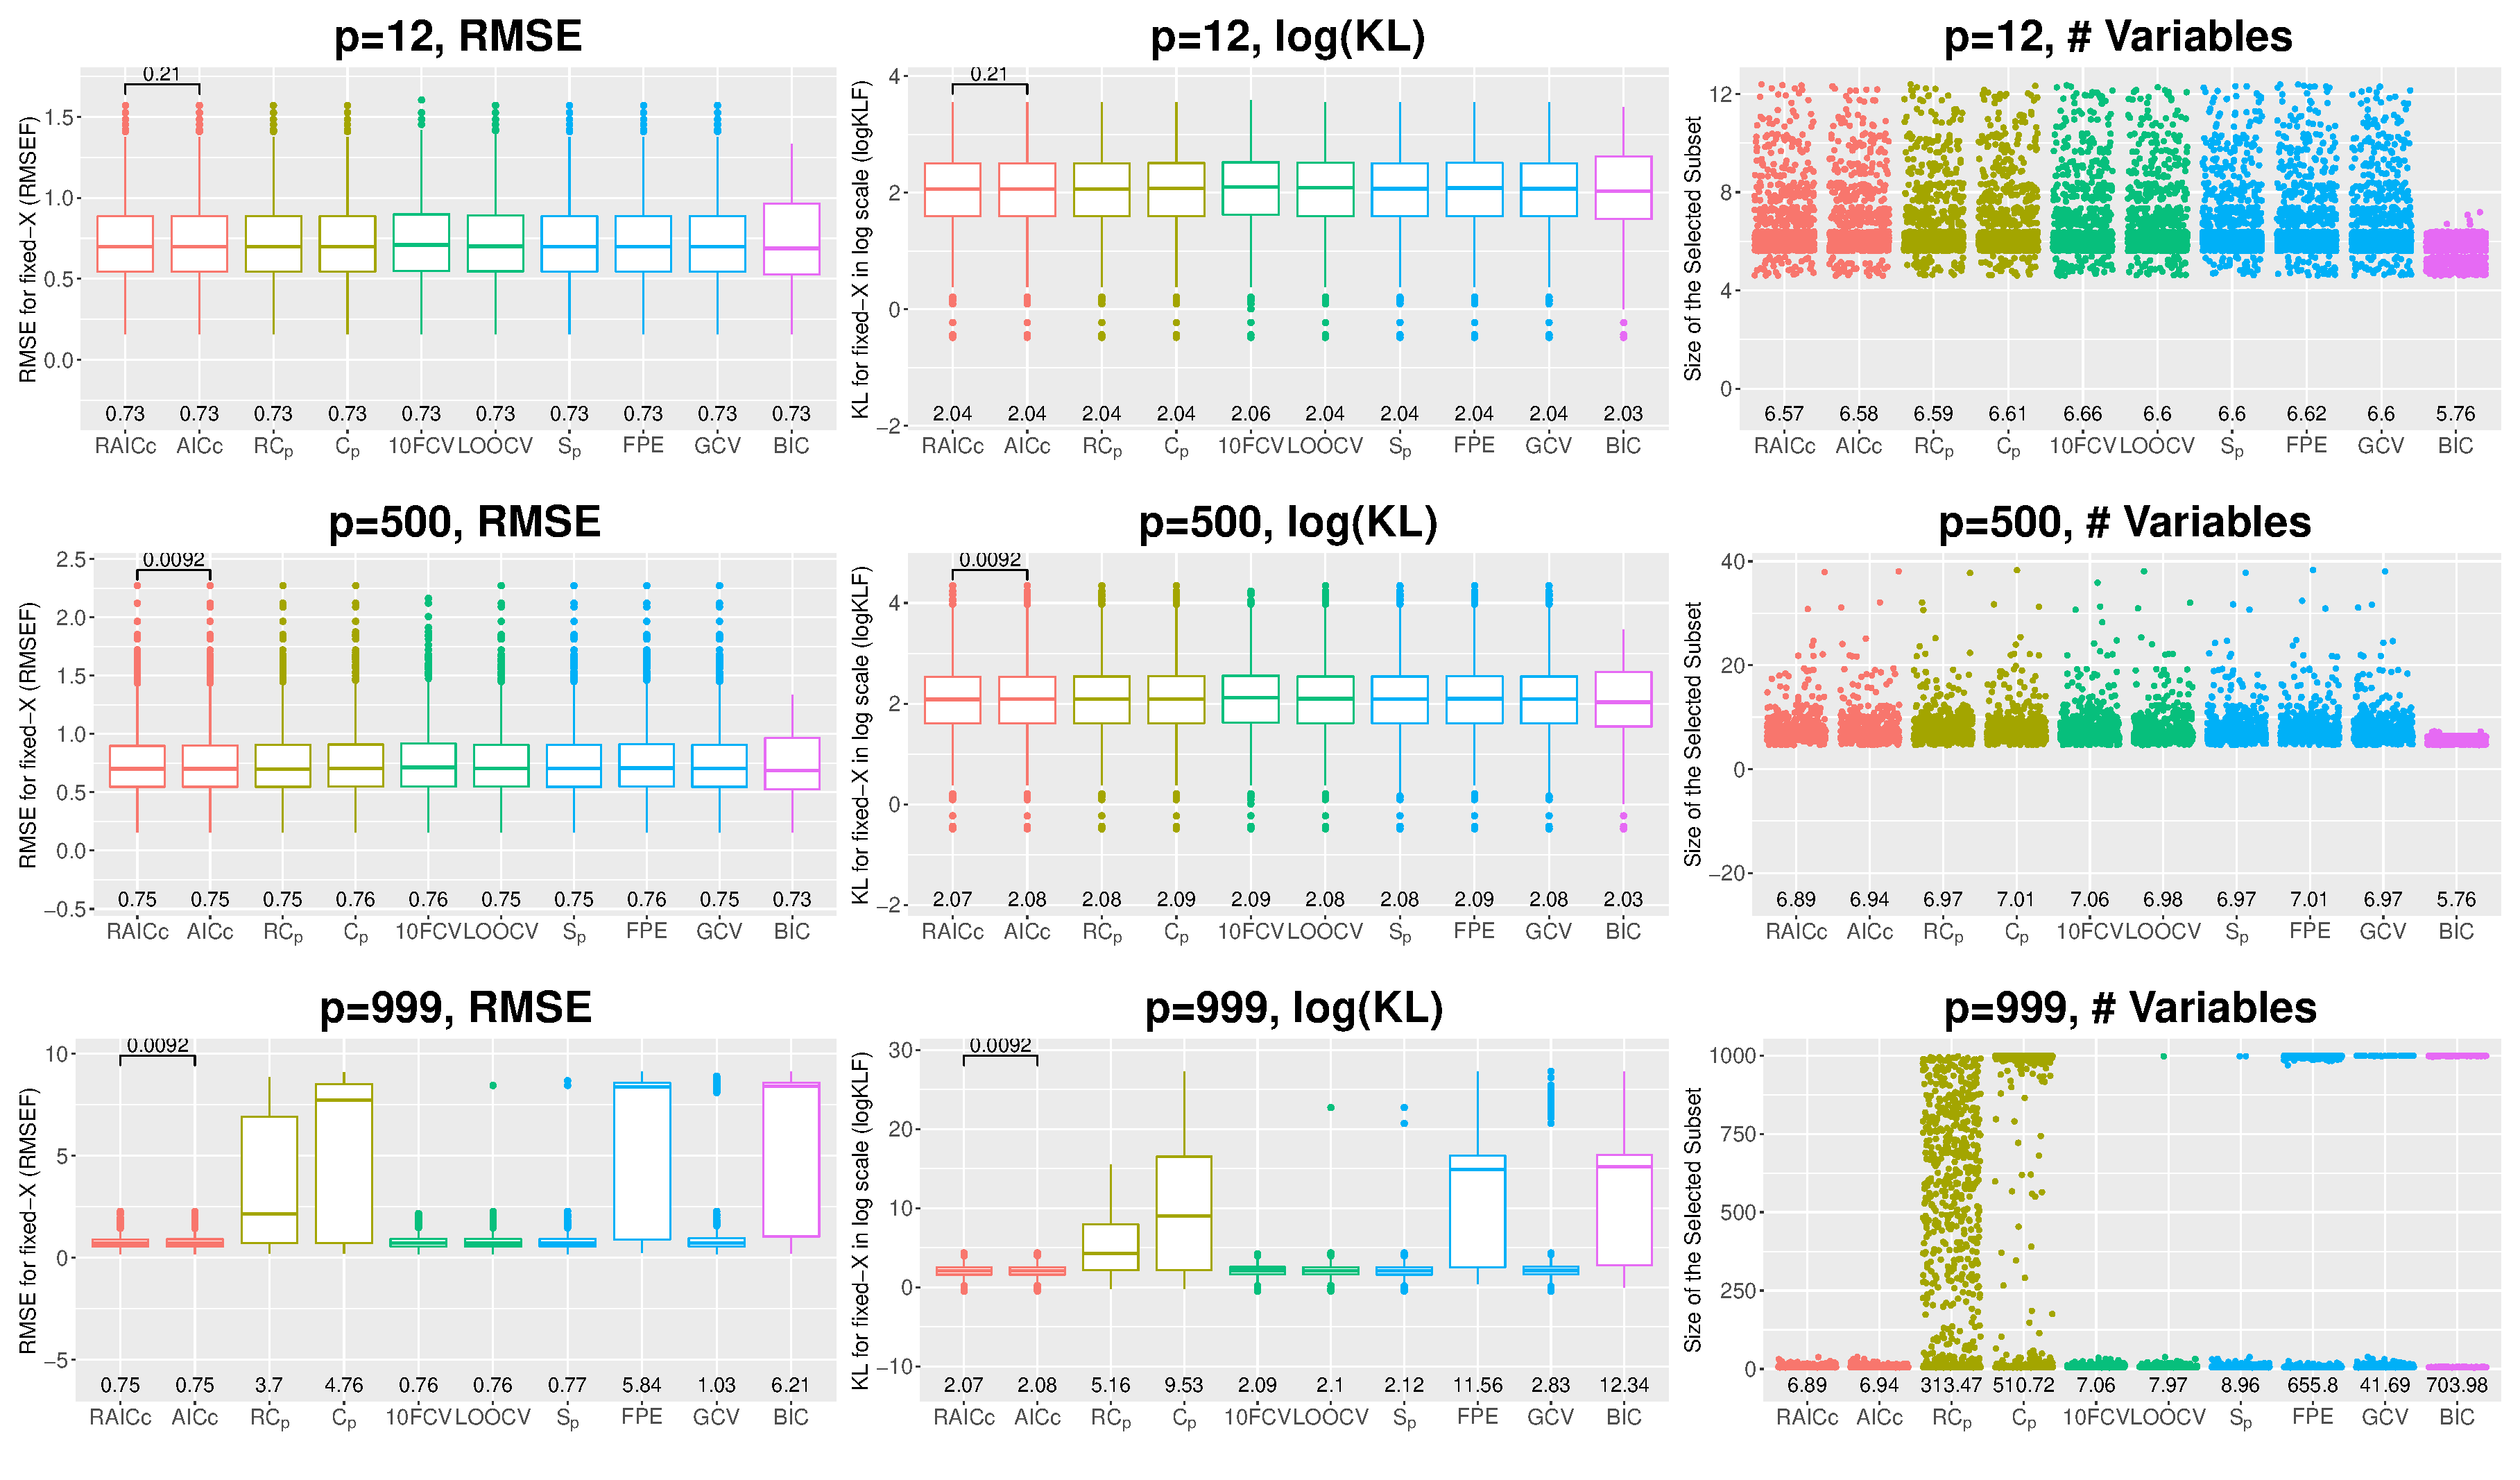
\includegraphics[width=\textwidth]{figures/supplement/fixedx_VS-Ex1_n1000_msnr_rho05.eps}
\caption{VS-Ex1, $n=1000$, medium signal, $\rho=0.5$, and Fixed-X.}
\end{figure}
\clearpage
\begin{figure}[!ht]
\centering
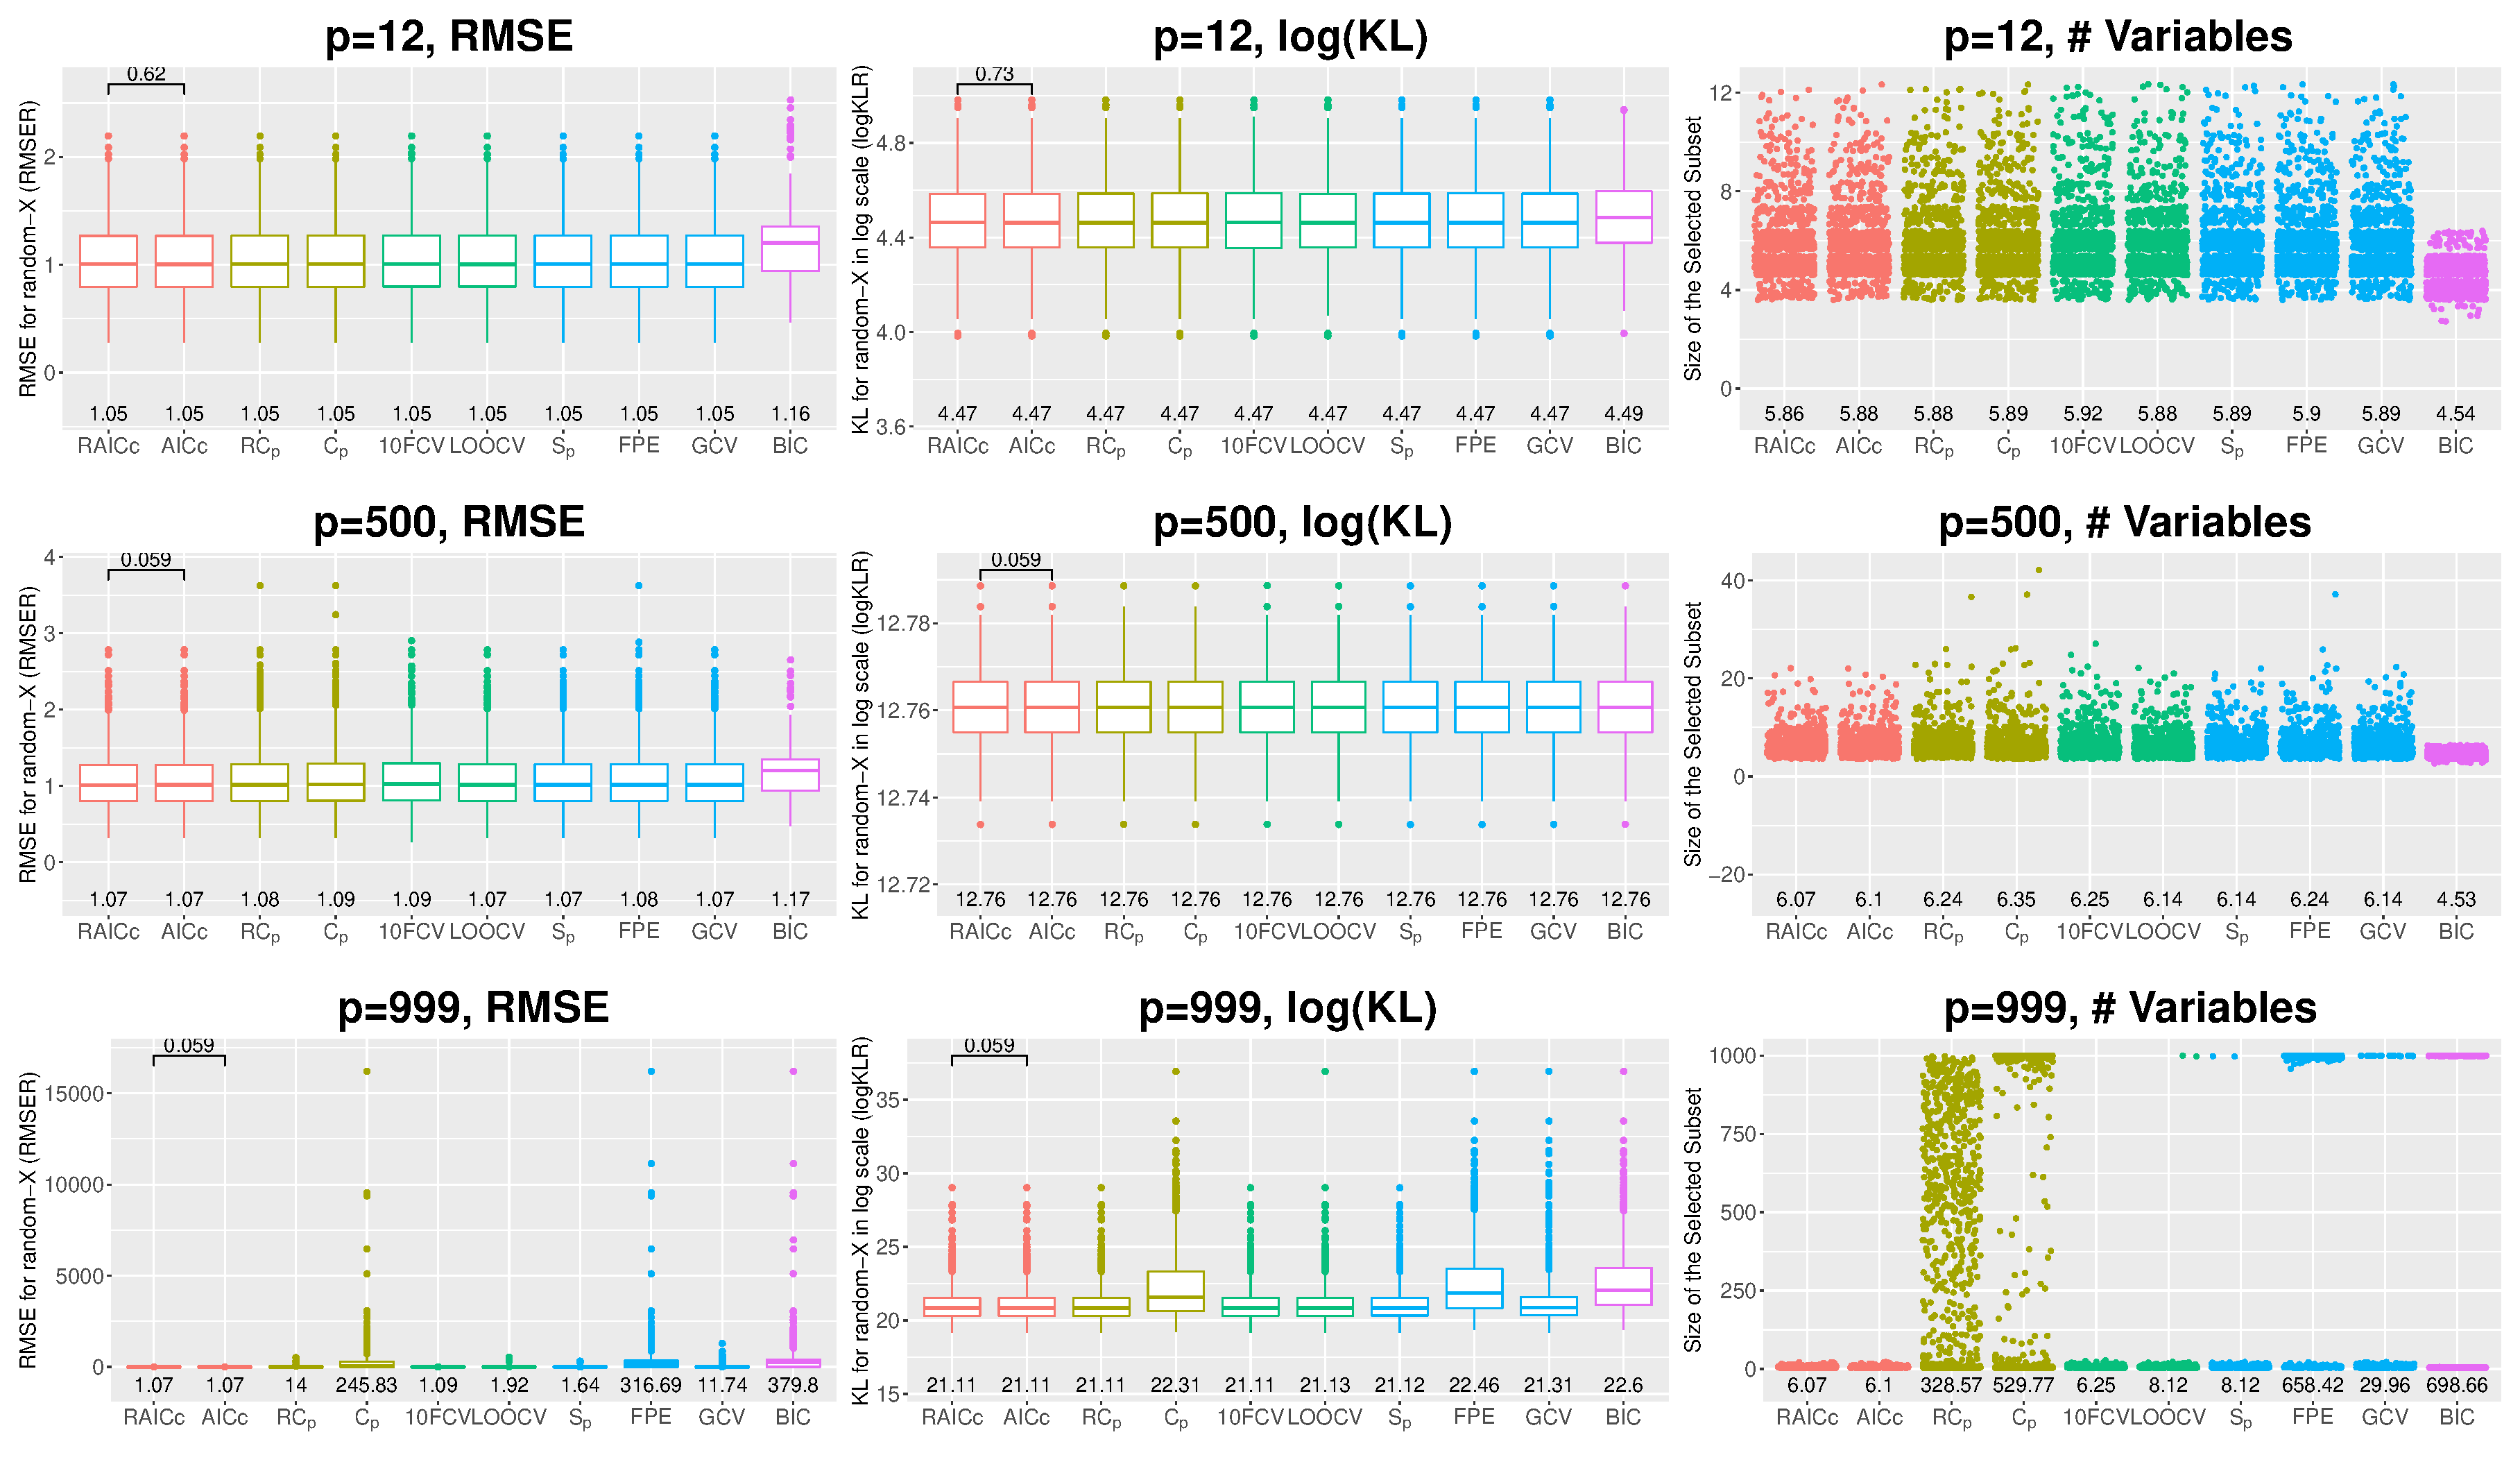
\includegraphics[width=\textwidth]{figures/supplement/randomx_VS-Ex1_n1000_msnr_rho09.eps}
\caption{VS-Ex1, $n=1000$, medium signal, $\rho=0.9$, and Random-X.}
\end{figure}
\begin{figure}[!ht]
\centering
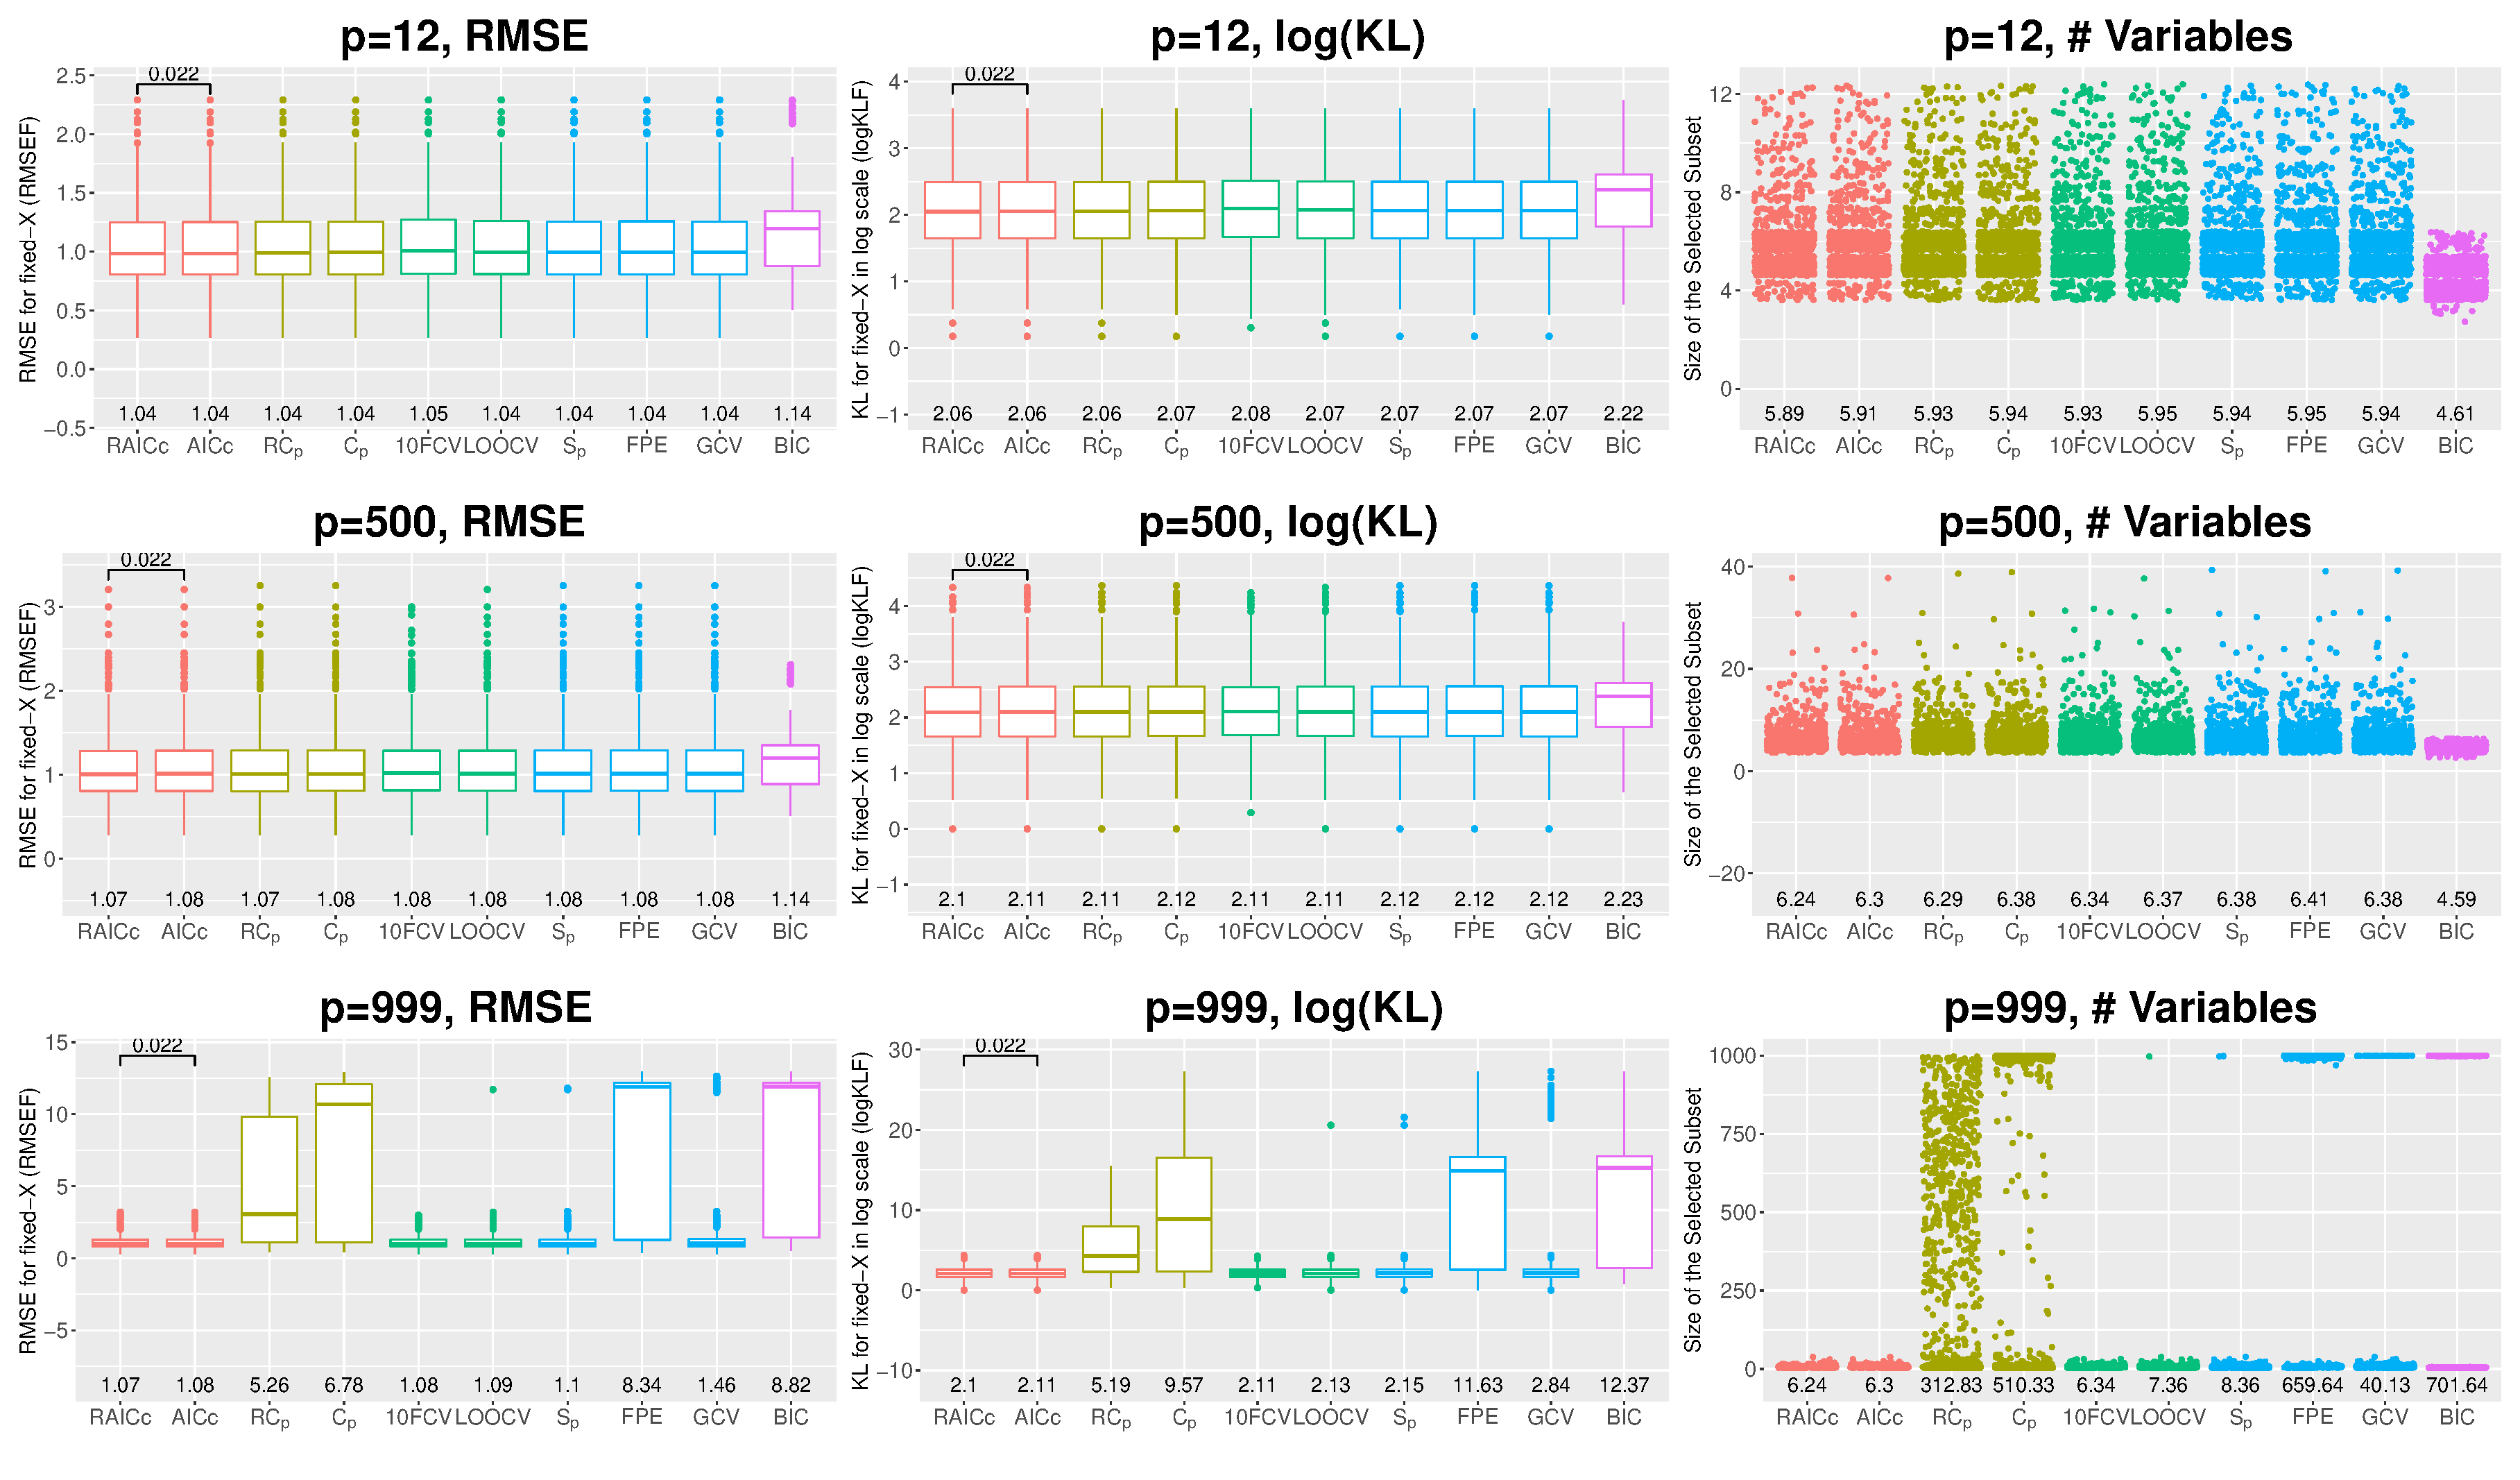
\includegraphics[width=\textwidth]{figures/supplement/fixedx_VS-Ex1_n1000_msnr_rho09.eps}
\caption{VS-Ex1, $n=1000$, medium signal, $\rho=0.9$, and Fixed-X.}
\end{figure}
\clearpage
\begin{figure}[!ht]
\centering
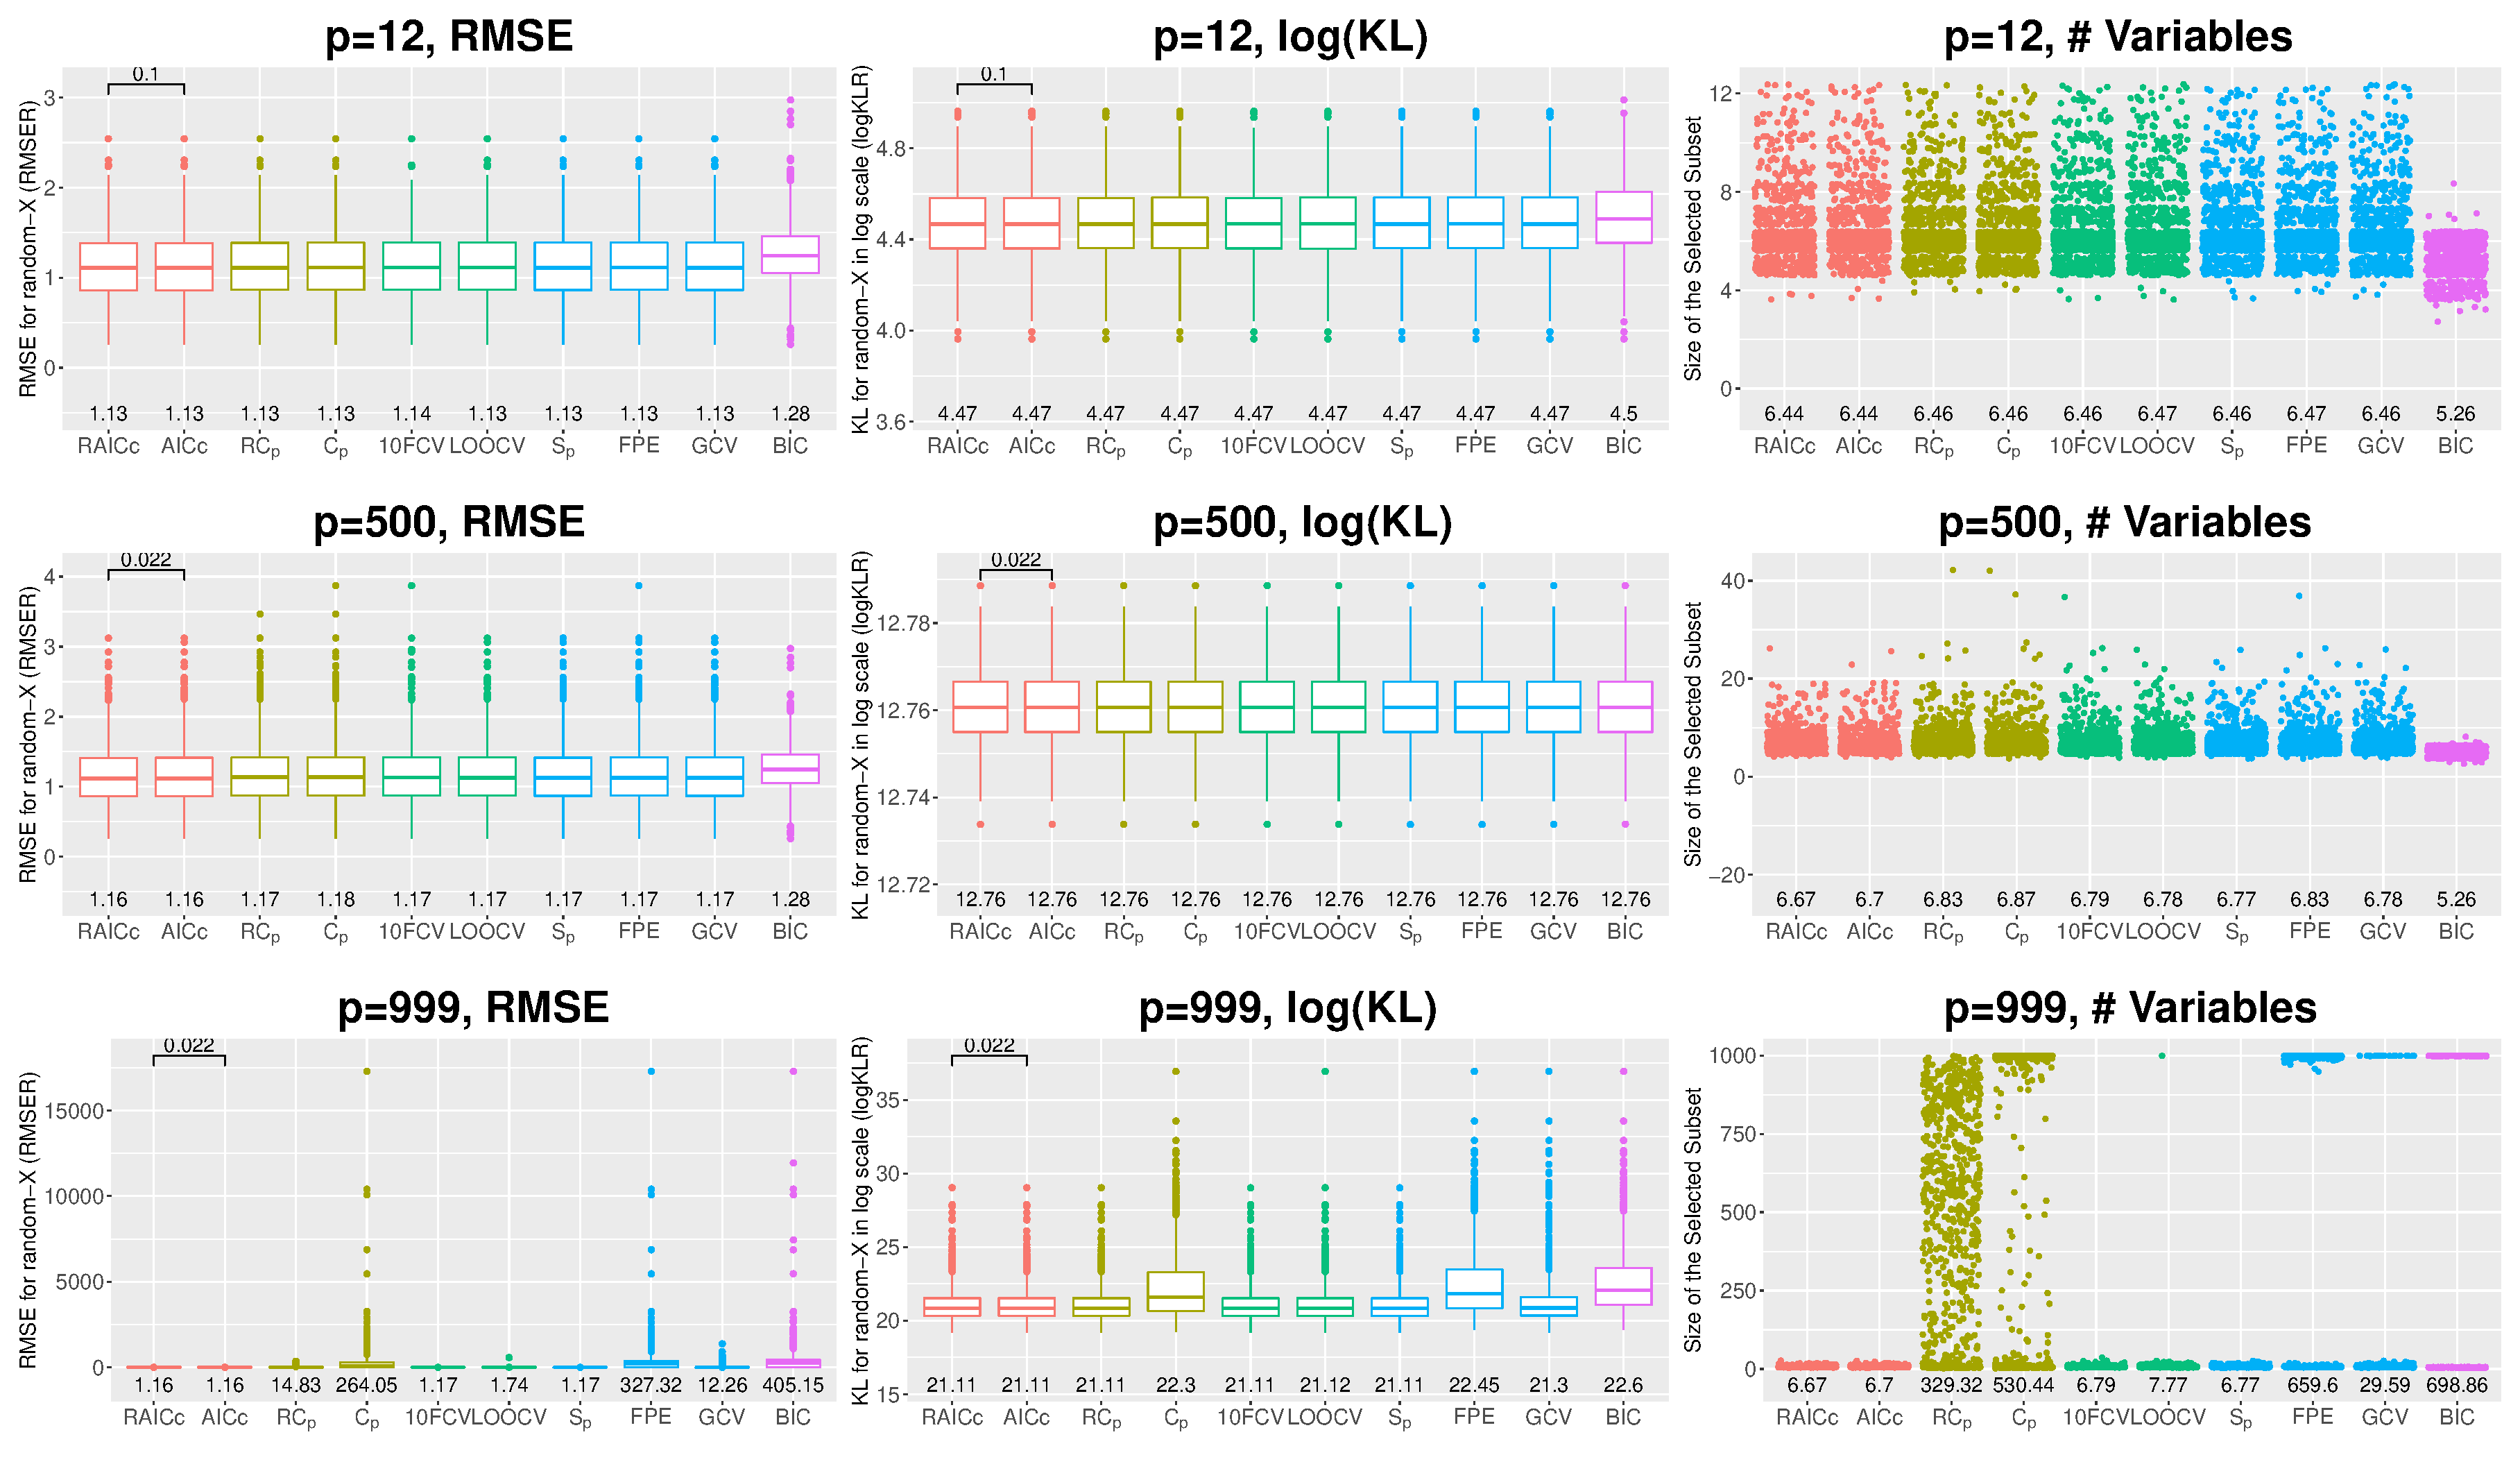
\includegraphics[width=\textwidth]{figures/supplement/randomx_VS-Ex1_n1000_lsnr_rho0.eps}
\caption{VS-Ex1, $n=1000$, low signal, $\rho=0$, and Random-X.}
\end{figure}
\begin{figure}[!ht]
\centering
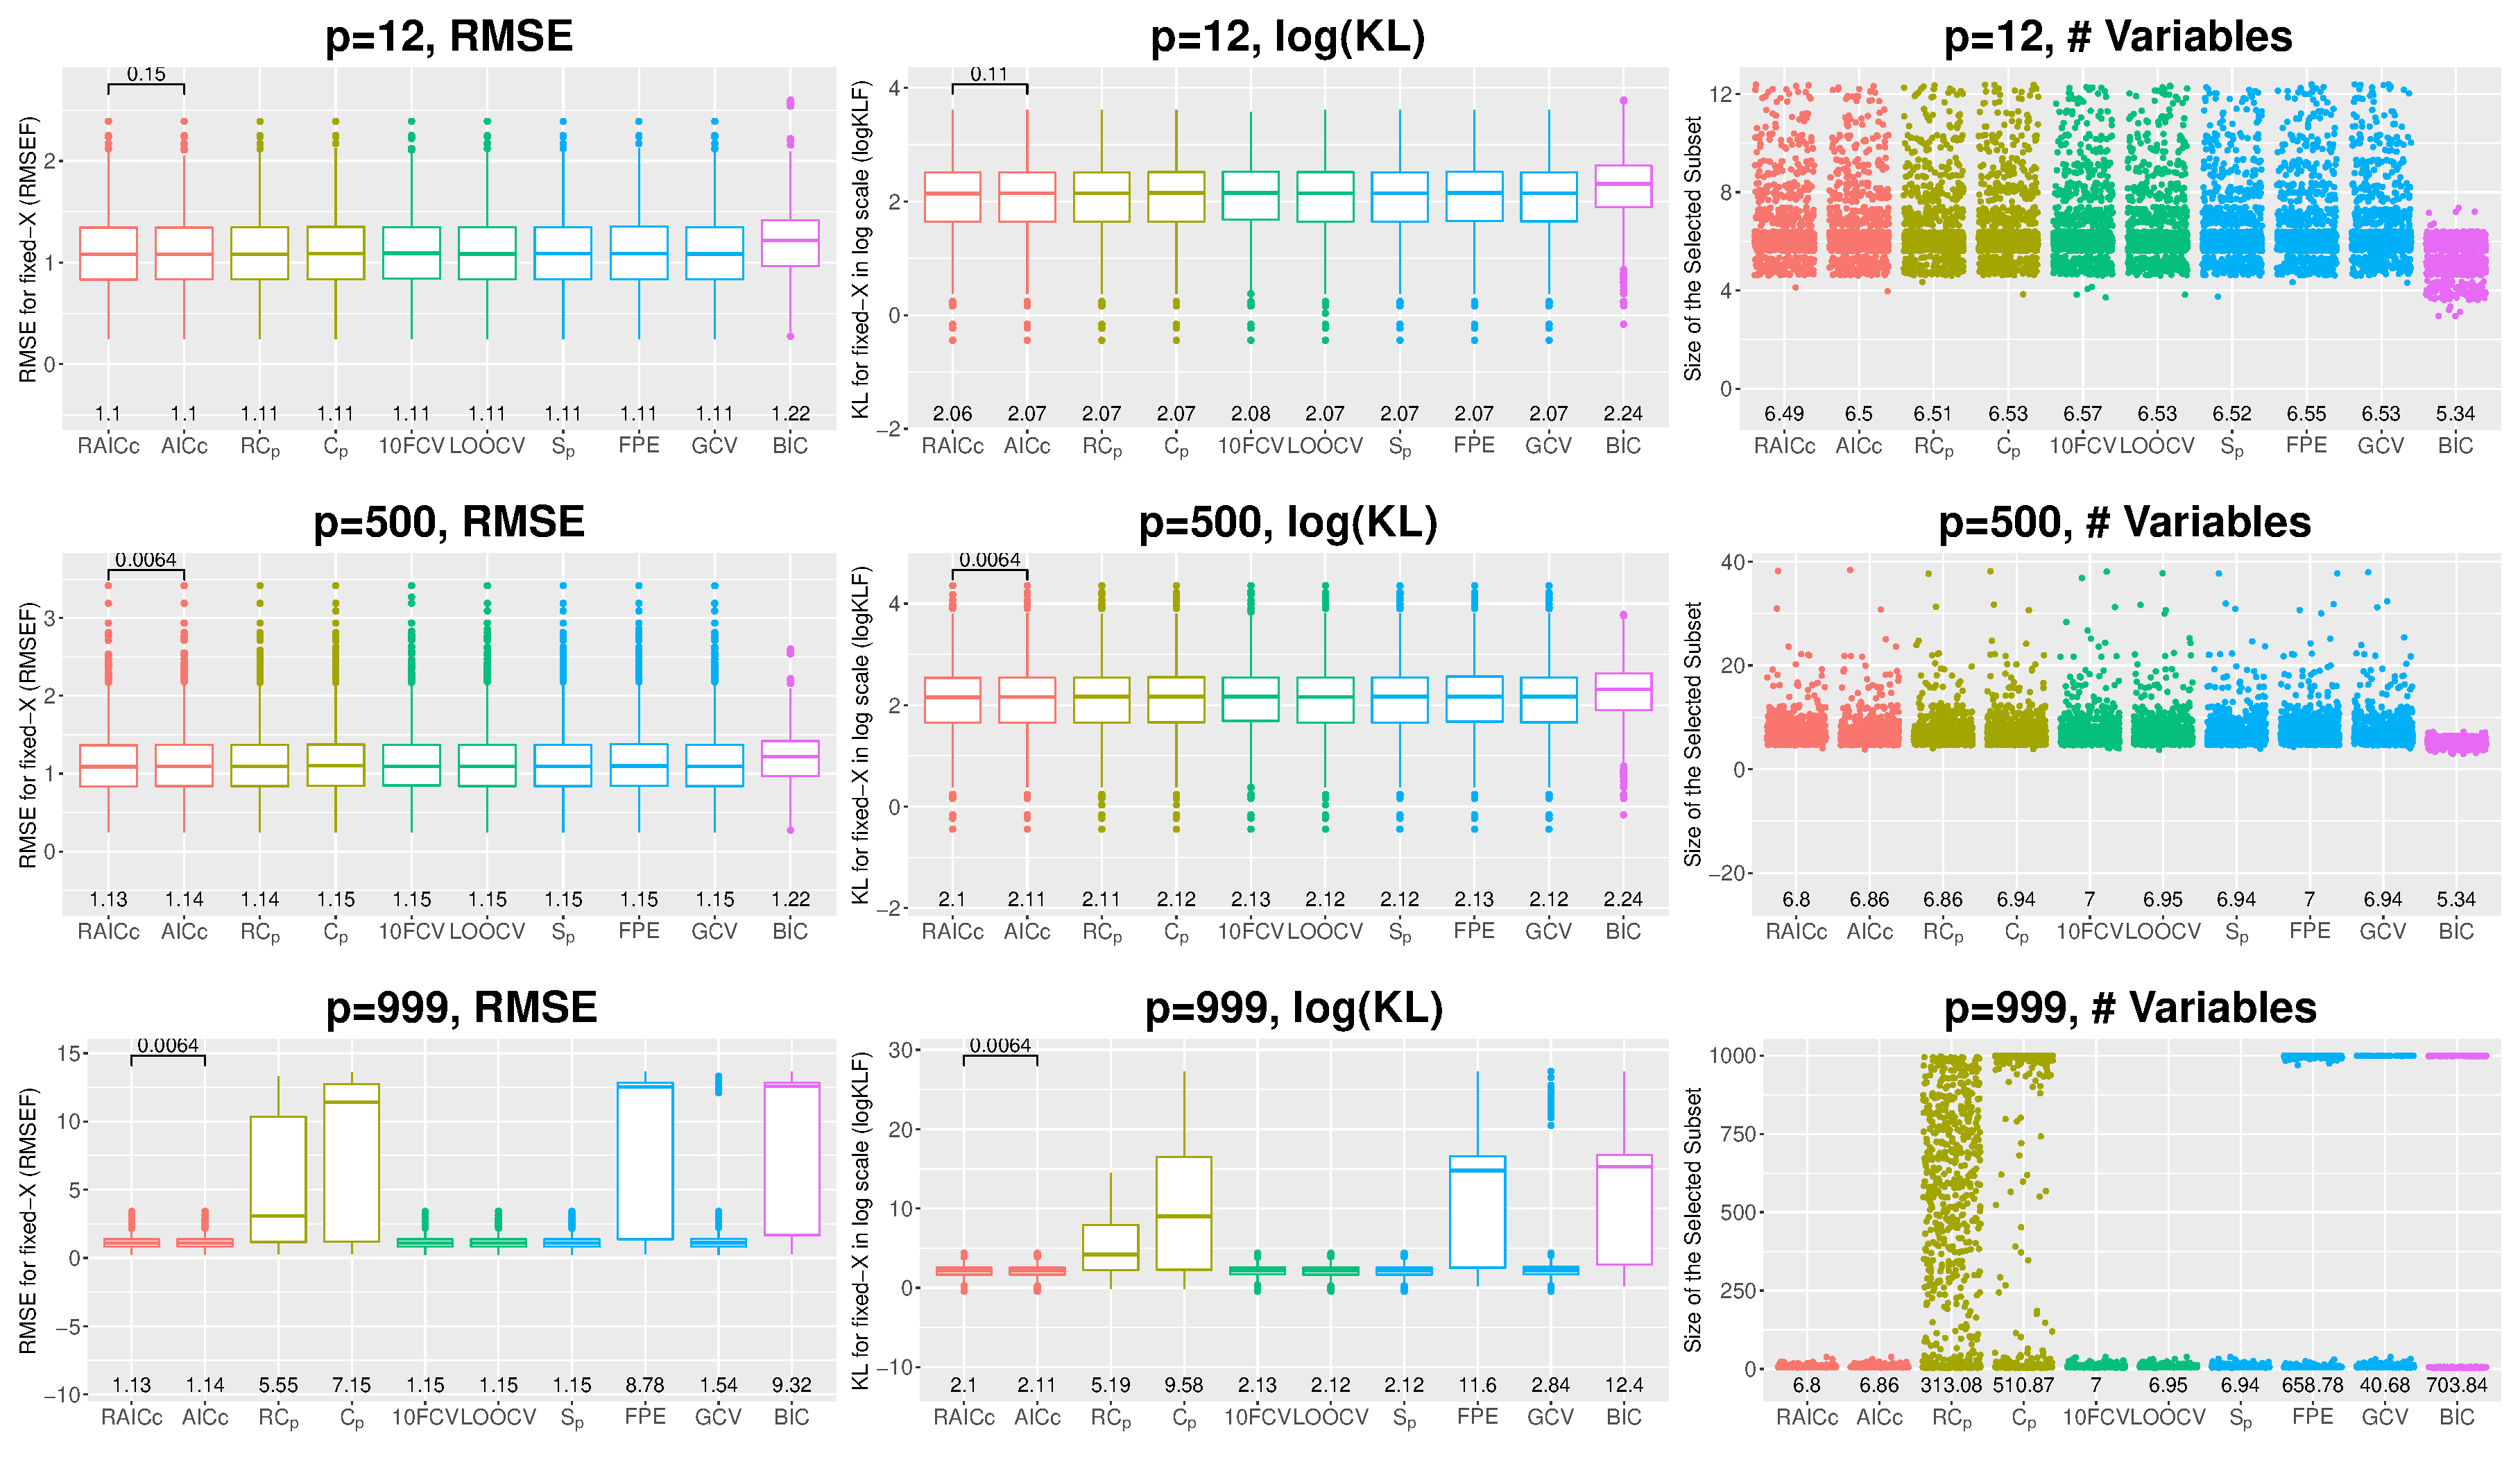
\includegraphics[width=\textwidth]{figures/supplement/fixedx_VS-Ex1_n1000_lsnr_rho0.eps}
\caption{VS-Ex1, $n=1000$, low signal, $\rho=0$, and Fixed-X.}
\end{figure}
\clearpage
\begin{figure}[!ht]
\centering
\includegraphics[width=\textwidth]{figures/supplement/randomx_VS-Ex1_n1000_lsnr_rho05.eps}
\caption{VS-Ex1, $n=1000$, low signal, $\rho=0.5$, and Random-X.}
\end{figure}
\begin{figure}[!ht]
\centering
\includegraphics[width=\textwidth]{figures/supplement/fixedx_VS-Ex1_n1000_lsnr_rho05.eps}
\caption{VS-Ex1, $n=1000$, low signal, $\rho=0.5$, and Fixed-X.}
\end{figure}
\clearpage
\begin{figure}[!ht]
\centering
\includegraphics[width=\textwidth]{figures/supplement/randomx_VS-Ex1_n1000_lsnr_rho09.eps}
\caption{VS-Ex1, $n=1000$, low signal, $\rho=0.9$, and Random-X.}
\end{figure}
\begin{figure}[!ht]
\centering
\includegraphics[width=\textwidth]{figures/supplement/fixedx_VS-Ex1_n1000_lsnr_rho09.eps}
\caption{VS-Ex1, $n=1000$, low signal, $\rho=0.9$, and Fixed-X.}
\end{figure}
\clearpage
\begin{figure}[!ht]
\centering
\includegraphics[width=\textwidth]{figures/supplement/randomx_VS-Ex2_n40_hsnr_rho0.eps}
\caption{VS-Ex2, $n=40$, high signal, $\rho=0$, and Random-X.}
\end{figure}
\begin{figure}[!ht]
\centering
\includegraphics[width=\textwidth]{figures/supplement/fixedx_VS-Ex2_n40_hsnr_rho0.eps}
\caption{VS-Ex2, $n=40$, high signal, $\rho=0$, and Fixed-X.}
\end{figure}
\clearpage
\begin{figure}[!ht]
\centering
\includegraphics[width=\textwidth]{figures/supplement/randomx_VS-Ex2_n40_hsnr_rho05.eps}
\caption{VS-Ex2, $n=40$, high signal, $\rho=0.5$, and Random-X.}
\end{figure}
\begin{figure}[!ht]
\centering
\includegraphics[width=\textwidth]{figures/supplement/fixedx_VS-Ex2_n40_hsnr_rho05.eps}
\caption{VS-Ex2, $n=40$, high signal, $\rho=0.5$, and Fixed-X.}
\end{figure}
\clearpage
\begin{figure}[!ht]
\centering
\includegraphics[width=\textwidth]{figures/supplement/randomx_VS-Ex2_n40_hsnr_rho09.eps}
\caption{VS-Ex2, $n=40$, high signal, $\rho=0.9$, and Random-X.}
\end{figure}
\begin{figure}[!ht]
\centering
\includegraphics[width=\textwidth]{figures/supplement/fixedx_VS-Ex2_n40_hsnr_rho09.eps}
\caption{VS-Ex2, $n=40$, high signal, $\rho=0.9$, and Fixed-X.}
\end{figure}
\clearpage
\begin{figure}[!ht]
\centering
\includegraphics[width=\textwidth]{figures/supplement/randomx_VS-Ex2_n40_msnr_rho0.eps}
\caption{VS-Ex2, $n=40$, medium signal, $\rho=0$, and Random-X.}
\end{figure}
\begin{figure}[!ht]
\centering
\includegraphics[width=\textwidth]{figures/supplement/fixedx_VS-Ex2_n40_msnr_rho0.eps}
\caption{VS-Ex2, $n=40$, medium signal, $\rho=0$, and Fixed-X.}
\end{figure}
\clearpage
\begin{figure}[!ht]
\centering
\includegraphics[width=\textwidth]{figures/supplement/randomx_VS-Ex2_n40_msnr_rho05.eps}
\caption{VS-Ex2, $n=40$, medium signal, $\rho=0.5$, and Random-X.}
\end{figure}
\begin{figure}[!ht]
\centering
\includegraphics[width=\textwidth]{figures/supplement/fixedx_VS-Ex2_n40_msnr_rho05.eps}
\caption{VS-Ex2, $n=40$, medium signal, $\rho=0.5$, and Fixed-X.}
\end{figure}
\clearpage
\begin{figure}[!ht]
\centering
\includegraphics[width=\textwidth]{figures/supplement/randomx_VS-Ex2_n40_msnr_rho09.eps}
\caption{VS-Ex2, $n=40$, medium signal, $\rho=0.9$, and Random-X.}
\end{figure}
\begin{figure}[!ht]
\centering
\includegraphics[width=\textwidth]{figures/supplement/fixedx_VS-Ex2_n40_msnr_rho09.eps}
\caption{VS-Ex2, $n=40$, medium signal, $\rho=0.9$, and Fixed-X.}
\end{figure}
\clearpage
\begin{figure}[!ht]
\centering
\includegraphics[width=\textwidth]{figures/supplement/randomx_VS-Ex2_n40_lsnr_rho0.eps}
\caption{VS-Ex2, $n=40$, low signal, $\rho=0$, and Random-X.}
\end{figure}
\begin{figure}[!ht]
\centering
\includegraphics[width=\textwidth]{figures/supplement/fixedx_VS-Ex2_n40_lsnr_rho0.eps}
\caption{VS-Ex2, $n=40$, low signal, $\rho=0$, and Fixed-X.}
\end{figure}
\clearpage
\begin{figure}[!ht]
\centering
\includegraphics[width=\textwidth]{figures/supplement/randomx_VS-Ex2_n40_lsnr_rho05.eps}
\caption{VS-Ex2, $n=40$, low signal, $\rho=0.5$, and Random-X.}
\end{figure}
\begin{figure}[!ht]
\centering
\includegraphics[width=\textwidth]{figures/supplement/fixedx_VS-Ex2_n40_lsnr_rho05.eps}
\caption{VS-Ex2, $n=40$, low signal, $\rho=0.5$, and Fixed-X.}
\end{figure}
\clearpage
\begin{figure}[!ht]
\centering
\includegraphics[width=\textwidth]{figures/supplement/randomx_VS-Ex2_n40_lsnr_rho09.eps}
\caption{VS-Ex2, $n=40$, low signal, $\rho=0.9$, and Random-X.}
\end{figure}
\begin{figure}[!ht]
\centering
\includegraphics[width=\textwidth]{figures/supplement/fixedx_VS-Ex2_n40_lsnr_rho09.eps}
\caption{VS-Ex2, $n=40$, low signal, $\rho=0.9$, and Fixed-X.}
\end{figure}
\clearpage
\begin{figure}[!ht]
\centering
\includegraphics[width=\textwidth]{figures/supplement/randomx_VS-Ex2_n200_hsnr_rho0.eps}
\caption{VS-Ex2, $n=200$, high signal, $\rho=0$, and Random-X.}
\end{figure}
\begin{figure}[!ht]
\centering
\includegraphics[width=\textwidth]{figures/supplement/fixedx_VS-Ex2_n200_hsnr_rho0.eps}
\caption{VS-Ex2, $n=200$, high signal, $\rho=0$, and Fixed-X.}
\end{figure}
\clearpage
\begin{figure}[!ht]
\centering
\includegraphics[width=\textwidth]{figures/supplement/randomx_VS-Ex2_n200_hsnr_rho05.eps}
\caption{VS-Ex2, $n=200$, high signal, $\rho=0.5$, and Random-X.}
\end{figure}
\begin{figure}[!ht]
\centering
\includegraphics[width=\textwidth]{figures/supplement/fixedx_VS-Ex2_n200_hsnr_rho05.eps}
\caption{VS-Ex2, $n=200$, high signal, $\rho=0.5$, and Fixed-X.}
\end{figure}
\clearpage
\begin{figure}[!ht]
\centering
\includegraphics[width=\textwidth]{figures/supplement/randomx_VS-Ex2_n200_hsnr_rho09.eps}
\caption{VS-Ex2, $n=200$, high signal, $\rho=0.9$, and Random-X.}
\end{figure}
\begin{figure}[!ht]
\centering
\includegraphics[width=\textwidth]{figures/supplement/fixedx_VS-Ex2_n200_hsnr_rho09.eps}
\caption{VS-Ex2, $n=200$, high signal, $\rho=0.9$, and Fixed-X.}
\end{figure}
\clearpage
\begin{figure}[!ht]
\centering
\includegraphics[width=\textwidth]{figures/supplement/randomx_VS-Ex2_n200_msnr_rho0.eps}
\caption{VS-Ex2, $n=200$, medium signal, $\rho=0$, and Random-X.}
\end{figure}
\begin{figure}[!ht]
\centering
\includegraphics[width=\textwidth]{figures/supplement/fixedx_VS-Ex2_n200_msnr_rho0.eps}
\caption{VS-Ex2, $n=200$, medium signal, $\rho=0$, and Fixed-X.}
\end{figure}
\clearpage
\begin{figure}[!ht]
\centering
\includegraphics[width=\textwidth]{figures/supplement/randomx_VS-Ex2_n200_msnr_rho05.eps}
\caption{VS-Ex2, $n=200$, medium signal, $\rho=0.5$, and Random-X.}
\end{figure}
\begin{figure}[!ht]
\centering
\includegraphics[width=\textwidth]{figures/supplement/fixedx_VS-Ex2_n200_msnr_rho05.eps}
\caption{VS-Ex2, $n=200$, medium signal, $\rho=0.5$, and Fixed-X.}
\end{figure}
\clearpage
\begin{figure}[!ht]
\centering
\includegraphics[width=\textwidth]{figures/supplement/randomx_VS-Ex2_n200_msnr_rho09.eps}
\caption{VS-Ex2, $n=200$, medium signal, $\rho=0.9$, and Random-X.}
\end{figure}
\begin{figure}[!ht]
\centering
\includegraphics[width=\textwidth]{figures/supplement/fixedx_VS-Ex2_n200_msnr_rho09.eps}
\caption{VS-Ex2, $n=200$, medium signal, $\rho=0.9$, and Fixed-X.}
\end{figure}
\clearpage
\begin{figure}[!ht]
\centering
\includegraphics[width=\textwidth]{figures/supplement/randomx_VS-Ex2_n200_lsnr_rho0.eps}
\caption{VS-Ex2, $n=200$, low signal, $\rho=0$, and Random-X.}
\end{figure}
\begin{figure}[!ht]
\centering
\includegraphics[width=\textwidth]{figures/supplement/fixedx_VS-Ex2_n200_lsnr_rho0.eps}
\caption{VS-Ex2, $n=200$, low signal, $\rho=0$, and Fixed-X.}
\end{figure}
\clearpage
\begin{figure}[!ht]
\centering
\includegraphics[width=\textwidth]{figures/supplement/randomx_VS-Ex2_n200_lsnr_rho05.eps}
\caption{VS-Ex2, $n=200$, low signal, $\rho=0.5$, and Random-X.}
\end{figure}
\begin{figure}[!ht]
\centering
\includegraphics[width=\textwidth]{figures/supplement/fixedx_VS-Ex2_n200_lsnr_rho05.eps}
\caption{VS-Ex2, $n=200$, low signal, $\rho=0.5$, and Fixed-X.}
\end{figure}
\clearpage
\begin{figure}[!ht]
\centering
\includegraphics[width=\textwidth]{figures/supplement/randomx_VS-Ex2_n200_lsnr_rho09.eps}
\caption{VS-Ex2, $n=200$, low signal, $\rho=0.9$, and Random-X.}
\end{figure}
\begin{figure}[!ht]
\centering
\includegraphics[width=\textwidth]{figures/supplement/fixedx_VS-Ex2_n200_lsnr_rho09.eps}
\caption{VS-Ex2, $n=200$, low signal, $\rho=0.9$, and Fixed-X.}
\end{figure}
\clearpage
\begin{figure}[!ht]
\centering
\includegraphics[width=\textwidth]{figures/supplement/randomx_VS-Ex2_n1000_hsnr_rho0.eps}
\caption{VS-Ex2, $n=1000$, high signal, $\rho=0$, and Random-X.}
\end{figure}
\begin{figure}[!ht]
\centering
\includegraphics[width=\textwidth]{figures/supplement/fixedx_VS-Ex2_n1000_hsnr_rho0.eps}
\caption{VS-Ex2, $n=1000$, high signal, $\rho=0$, and Fixed-X.}
\end{figure}
\clearpage
\begin{figure}[!ht]
\centering
\includegraphics[width=\textwidth]{figures/supplement/randomx_VS-Ex2_n1000_hsnr_rho05.eps}
\caption{VS-Ex2, $n=1000$, high signal, $\rho=0.5$, and Random-X.}
\end{figure}
\begin{figure}[!ht]
\centering
\includegraphics[width=\textwidth]{figures/supplement/fixedx_VS-Ex2_n1000_hsnr_rho05.eps}
\caption{VS-Ex2, $n=1000$, high signal, $\rho=0.5$, and Fixed-X.}
\end{figure}
\clearpage
\begin{figure}[!ht]
\centering
\includegraphics[width=\textwidth]{figures/supplement/randomx_VS-Ex2_n1000_hsnr_rho09.eps}
\caption{VS-Ex2, $n=1000$, high signal, $\rho=0.9$, and Random-X.}
\end{figure}
\begin{figure}[!ht]
\centering
\includegraphics[width=\textwidth]{figures/supplement/fixedx_VS-Ex2_n1000_hsnr_rho09.eps}
\caption{VS-Ex2, $n=1000$, high signal, $\rho=0.9$, and Fixed-X.}
\end{figure}
\clearpage
\begin{figure}[!ht]
\centering
\includegraphics[width=\textwidth]{figures/supplement/randomx_VS-Ex2_n1000_msnr_rho0.eps}
\caption{VS-Ex2, $n=1000$, medium signal, $\rho=0$, and Random-X.}
\end{figure}
\begin{figure}[!ht]
\centering
\includegraphics[width=\textwidth]{figures/supplement/fixedx_VS-Ex2_n1000_msnr_rho0.eps}
\caption{VS-Ex2, $n=1000$, medium signal, $\rho=0$, and Fixed-X.}
\end{figure}
\clearpage
\begin{figure}[!ht]
\centering
\includegraphics[width=\textwidth]{figures/supplement/randomx_VS-Ex2_n1000_msnr_rho05.eps}
\caption{VS-Ex2, $n=1000$, medium signal, $\rho=0.5$, and Random-X.}
\end{figure}
\begin{figure}[!ht]
\centering
\includegraphics[width=\textwidth]{figures/supplement/fixedx_VS-Ex2_n1000_msnr_rho05.eps}
\caption{VS-Ex2, $n=1000$, medium signal, $\rho=0.5$, and Fixed-X.}
\end{figure}
\clearpage
\begin{figure}[!ht]
\centering
\includegraphics[width=\textwidth]{figures/supplement/randomx_VS-Ex2_n1000_msnr_rho09.eps}
\caption{VS-Ex2, $n=1000$, medium signal, $\rho=0.9$, and Random-X.}
\end{figure}
\begin{figure}[!ht]
\centering
\includegraphics[width=\textwidth]{figures/supplement/fixedx_VS-Ex2_n1000_msnr_rho09.eps}
\caption{VS-Ex2, $n=1000$, medium signal, $\rho=0.9$, and Fixed-X.}
\end{figure}
\clearpage
\begin{figure}[!ht]
\centering
\includegraphics[width=\textwidth]{figures/supplement/randomx_VS-Ex2_n1000_lsnr_rho0.eps}
\caption{VS-Ex2, $n=1000$, low signal, $\rho=0$, and Random-X.}
\end{figure}
\begin{figure}[!ht]
\centering
\includegraphics[width=\textwidth]{figures/supplement/fixedx_VS-Ex2_n1000_lsnr_rho0.eps}
\caption{VS-Ex2, $n=1000$, low signal, $\rho=0$, and Fixed-X.}
\end{figure}
\clearpage
\begin{figure}[!ht]
\centering
\includegraphics[width=\textwidth]{figures/supplement/randomx_VS-Ex2_n1000_lsnr_rho05.eps}
\caption{VS-Ex2, $n=1000$, low signal, $\rho=0.5$, and Random-X.}
\end{figure}
\begin{figure}[!ht]
\centering
\includegraphics[width=\textwidth]{figures/supplement/fixedx_VS-Ex2_n1000_lsnr_rho05.eps}
\caption{VS-Ex2, $n=1000$, low signal, $\rho=0.5$, and Fixed-X.}
\end{figure}
\clearpage
\begin{figure}[!ht]
\centering
\includegraphics[width=\textwidth]{figures/supplement/randomx_VS-Ex2_n1000_lsnr_rho09.eps}
\caption{VS-Ex2, $n=1000$, low signal, $\rho=0.9$, and Random-X.}
\end{figure}
\begin{figure}[!ht]
\centering
\includegraphics[width=\textwidth]{figures/supplement/fixedx_VS-Ex2_n1000_lsnr_rho09.eps}
\caption{VS-Ex2, $n=1000$, low signal, $\rho=0.9$, and Fixed-X.}
\end{figure}
\clearpage
\begin{figure}[!ht]
\centering
\includegraphics[width=\textwidth]{figures/supplement/randomx_VS-Ex3_n40_hsnr_rho0.eps}
\caption{VS-Ex3, $n=40$, high signal, $\rho=0$, and Random-X.}
\end{figure}
\begin{figure}[!ht]
\centering
\includegraphics[width=\textwidth]{figures/supplement/fixedx_VS-Ex3_n40_hsnr_rho0.eps}
\caption{VS-Ex3, $n=40$, high signal, $\rho=0$, and Fixed-X.}
\end{figure}
\clearpage
\begin{figure}[!ht]
\centering
\includegraphics[width=\textwidth]{figures/supplement/randomx_VS-Ex3_n40_hsnr_rho05.eps}
\caption{VS-Ex3, $n=40$, high signal, $\rho=0.5$, and Random-X.}
\end{figure}
\begin{figure}[!ht]
\centering
\includegraphics[width=\textwidth]{figures/supplement/fixedx_VS-Ex3_n40_hsnr_rho05.eps}
\caption{VS-Ex3, $n=40$, high signal, $\rho=0.5$, and Fixed-X.}
\end{figure}
\clearpage
\begin{figure}[!ht]
\centering
\includegraphics[width=\textwidth]{figures/supplement/randomx_VS-Ex3_n40_hsnr_rho09.eps}
\caption{VS-Ex3, $n=40$, high signal, $\rho=0.9$, and Random-X.}
\end{figure}
\begin{figure}[!ht]
\centering
\includegraphics[width=\textwidth]{figures/supplement/fixedx_VS-Ex3_n40_hsnr_rho09.eps}
\caption{VS-Ex3, $n=40$, high signal, $\rho=0.9$, and Fixed-X.}
\end{figure}
\clearpage
\begin{figure}[!ht]
\centering
\includegraphics[width=\textwidth]{figures/supplement/randomx_VS-Ex3_n40_msnr_rho0.eps}
\caption{VS-Ex3, $n=40$, medium signal, $\rho=0$, and Random-X.}
\end{figure}
\begin{figure}[!ht]
\centering
\includegraphics[width=\textwidth]{figures/supplement/fixedx_VS-Ex3_n40_msnr_rho0.eps}
\caption{VS-Ex3, $n=40$, medium signal, $\rho=0$, and Fixed-X.}
\end{figure}
\clearpage
\begin{figure}[!ht]
\centering
\includegraphics[width=\textwidth]{figures/supplement/randomx_VS-Ex3_n40_msnr_rho05.eps}
\caption{VS-Ex3, $n=40$, medium signal, $\rho=0.5$, and Random-X.}
\end{figure}
\begin{figure}[!ht]
\centering
\includegraphics[width=\textwidth]{figures/supplement/fixedx_VS-Ex3_n40_msnr_rho05.eps}
\caption{VS-Ex3, $n=40$, medium signal, $\rho=0.5$, and Fixed-X.}
\end{figure}
\clearpage
\begin{figure}[!ht]
\centering
\includegraphics[width=\textwidth]{figures/supplement/randomx_VS-Ex3_n40_msnr_rho09.eps}
\caption{VS-Ex3, $n=40$, medium signal, $\rho=0.9$, and Random-X.}
\end{figure}
\begin{figure}[!ht]
\centering
\includegraphics[width=\textwidth]{figures/supplement/fixedx_VS-Ex3_n40_msnr_rho09.eps}
\caption{VS-Ex3, $n=40$, medium signal, $\rho=0.9$, and Fixed-X.}
\end{figure}
\clearpage
\begin{figure}[!ht]
\centering
\includegraphics[width=\textwidth]{figures/supplement/randomx_VS-Ex3_n40_lsnr_rho0.eps}
\caption{VS-Ex3, $n=40$, low signal, $\rho=0$, and Random-X.}
\end{figure}
\begin{figure}[!ht]
\centering
\includegraphics[width=\textwidth]{figures/supplement/fixedx_VS-Ex3_n40_lsnr_rho0.eps}
\caption{VS-Ex3, $n=40$, low signal, $\rho=0$, and Fixed-X.}
\end{figure}
\clearpage
\begin{figure}[!ht]
\centering
\includegraphics[width=\textwidth]{figures/supplement/randomx_VS-Ex3_n40_lsnr_rho05.eps}
\caption{VS-Ex3, $n=40$, low signal, $\rho=0.5$, and Random-X.}
\end{figure}
\begin{figure}[!ht]
\centering
\includegraphics[width=\textwidth]{figures/supplement/fixedx_VS-Ex3_n40_lsnr_rho05.eps}
\caption{VS-Ex3, $n=40$, low signal, $\rho=0.5$, and Fixed-X.}
\end{figure}
\clearpage
\begin{figure}[!ht]
\centering
\includegraphics[width=\textwidth]{figures/supplement/randomx_VS-Ex3_n40_lsnr_rho09.eps}
\caption{VS-Ex3, $n=40$, low signal, $\rho=0.9$, and Random-X.}
\end{figure}
\begin{figure}[!ht]
\centering
\includegraphics[width=\textwidth]{figures/supplement/fixedx_VS-Ex3_n40_lsnr_rho09.eps}
\caption{VS-Ex3, $n=40$, low signal, $\rho=0.9$, and Fixed-X.}
\end{figure}
\clearpage
\begin{figure}[!ht]
\centering
\includegraphics[width=\textwidth]{figures/supplement/randomx_VS-Ex3_n200_hsnr_rho0.eps}
\caption{VS-Ex3, $n=200$, high signal, $\rho=0$, and Random-X.}
\end{figure}
\begin{figure}[!ht]
\centering
\includegraphics[width=\textwidth]{figures/supplement/fixedx_VS-Ex3_n200_hsnr_rho0.eps}
\caption{VS-Ex3, $n=200$, high signal, $\rho=0$, and Fixed-X.}
\end{figure}
\clearpage
\begin{figure}[!ht]
\centering
\includegraphics[width=\textwidth]{figures/supplement/randomx_VS-Ex3_n200_hsnr_rho05.eps}
\caption{VS-Ex3, $n=200$, high signal, $\rho=0.5$, and Random-X.}
\end{figure}
\begin{figure}[!ht]
\centering
\includegraphics[width=\textwidth]{figures/supplement/fixedx_VS-Ex3_n200_hsnr_rho05.eps}
\caption{VS-Ex3, $n=200$, high signal, $\rho=0.5$, and Fixed-X.}
\end{figure}
\clearpage
\begin{figure}[!ht]
\centering
\includegraphics[width=\textwidth]{figures/supplement/randomx_VS-Ex3_n200_hsnr_rho09.eps}
\caption{VS-Ex3, $n=200$, high signal, $\rho=0.9$, and Random-X.}
\end{figure}
\begin{figure}[!ht]
\centering
\includegraphics[width=\textwidth]{figures/supplement/fixedx_VS-Ex3_n200_hsnr_rho09.eps}
\caption{VS-Ex3, $n=200$, high signal, $\rho=0.9$, and Fixed-X.}
\end{figure}
\clearpage
\begin{figure}[!ht]
\centering
\includegraphics[width=\textwidth]{figures/supplement/randomx_VS-Ex3_n200_msnr_rho0.eps}
\caption{VS-Ex3, $n=200$, medium signal, $\rho=0$, and Random-X.}
\end{figure}
\begin{figure}[!ht]
\centering
\includegraphics[width=\textwidth]{figures/supplement/fixedx_VS-Ex3_n200_msnr_rho0.eps}
\caption{VS-Ex3, $n=200$, medium signal, $\rho=0$, and Fixed-X.}
\end{figure}
\clearpage
\begin{figure}[!ht]
\centering
\includegraphics[width=\textwidth]{figures/supplement/randomx_VS-Ex3_n200_msnr_rho05.eps}
\caption{VS-Ex3, $n=200$, medium signal, $\rho=0.5$, and Random-X.}
\end{figure}
\begin{figure}[!ht]
\centering
\includegraphics[width=\textwidth]{figures/supplement/fixedx_VS-Ex3_n200_msnr_rho05.eps}
\caption{VS-Ex3, $n=200$, medium signal, $\rho=0.5$, and Fixed-X.}
\end{figure}
\clearpage
\begin{figure}[!ht]
\centering
\includegraphics[width=\textwidth]{figures/supplement/randomx_VS-Ex3_n200_msnr_rho09.eps}
\caption{VS-Ex3, $n=200$, medium signal, $\rho=0.9$, and Random-X.}
\end{figure}
\begin{figure}[!ht]
\centering
\includegraphics[width=\textwidth]{figures/supplement/fixedx_VS-Ex3_n200_msnr_rho09.eps}
\caption{VS-Ex3, $n=200$, medium signal, $\rho=0.9$, and Fixed-X.}
\end{figure}
\clearpage
\begin{figure}[!ht]
\centering
\includegraphics[width=\textwidth]{figures/supplement/randomx_VS-Ex3_n200_lsnr_rho0.eps}
\caption{VS-Ex3, $n=200$, low signal, $\rho=0$, and Random-X.}
\end{figure}
\begin{figure}[!ht]
\centering
\includegraphics[width=\textwidth]{figures/supplement/fixedx_VS-Ex3_n200_lsnr_rho0.eps}
\caption{VS-Ex3, $n=200$, low signal, $\rho=0$, and Fixed-X.}
\end{figure}
\clearpage
\begin{figure}[!ht]
\centering
\includegraphics[width=\textwidth]{figures/supplement/randomx_VS-Ex3_n200_lsnr_rho05.eps}
\caption{VS-Ex3, $n=200$, low signal, $\rho=0.5$, and Random-X.}
\end{figure}
\begin{figure}[!ht]
\centering
\includegraphics[width=\textwidth]{figures/supplement/fixedx_VS-Ex3_n200_lsnr_rho05.eps}
\caption{VS-Ex3, $n=200$, low signal, $\rho=0.5$, and Fixed-X.}
\end{figure}
\clearpage
\begin{figure}[!ht]
\centering
\includegraphics[width=\textwidth]{figures/supplement/randomx_VS-Ex3_n200_lsnr_rho09.eps}
\caption{VS-Ex3, $n=200$, low signal, $\rho=0.9$, and Random-X.}
\end{figure}
\begin{figure}[!ht]
\centering
\includegraphics[width=\textwidth]{figures/supplement/fixedx_VS-Ex3_n200_lsnr_rho09.eps}
\caption{VS-Ex3, $n=200$, low signal, $\rho=0.9$, and Fixed-X.}
\end{figure}
\clearpage
\begin{figure}[!ht]
\centering
\includegraphics[width=\textwidth]{figures/supplement/randomx_VS-Ex3_n1000_hsnr_rho0.eps}
\caption{VS-Ex3, $n=1000$, high signal, $\rho=0$, and Random-X.}
\end{figure}
\begin{figure}[!ht]
\centering
\includegraphics[width=\textwidth]{figures/supplement/fixedx_VS-Ex3_n1000_hsnr_rho0.eps}
\caption{VS-Ex3, $n=1000$, high signal, $\rho=0$, and Fixed-X.}
\end{figure}
\clearpage
\begin{figure}[!ht]
\centering
\includegraphics[width=\textwidth]{figures/supplement/randomx_VS-Ex3_n1000_hsnr_rho05.eps}
\caption{VS-Ex3, $n=1000$, high signal, $\rho=0.5$, and Random-X.}
\end{figure}
\begin{figure}[!ht]
\centering
\includegraphics[width=\textwidth]{figures/supplement/fixedx_VS-Ex3_n1000_hsnr_rho05.eps}
\caption{VS-Ex3, $n=1000$, high signal, $\rho=0.5$, and Fixed-X.}
\end{figure}
\clearpage
\begin{figure}[!ht]
\centering
\includegraphics[width=\textwidth]{figures/supplement/randomx_VS-Ex3_n1000_hsnr_rho09.eps}
\caption{VS-Ex3, $n=1000$, high signal, $\rho=0.9$, and Random-X.}
\end{figure}
\begin{figure}[!ht]
\centering
\includegraphics[width=\textwidth]{figures/supplement/fixedx_VS-Ex3_n1000_hsnr_rho09.eps}
\caption{VS-Ex3, $n=1000$, high signal, $\rho=0.9$, and Fixed-X.}
\end{figure}
\clearpage
\begin{figure}[!ht]
\centering
\includegraphics[width=\textwidth]{figures/supplement/randomx_VS-Ex3_n1000_msnr_rho0.eps}
\caption{VS-Ex3, $n=1000$, medium signal, $\rho=0$, and Random-X.}
\end{figure}
\begin{figure}[!ht]
\centering
\includegraphics[width=\textwidth]{figures/supplement/fixedx_VS-Ex3_n1000_msnr_rho0.eps}
\caption{VS-Ex3, $n=1000$, medium signal, $\rho=0$, and Fixed-X.}
\end{figure}
\clearpage
\begin{figure}[!ht]
\centering
\includegraphics[width=\textwidth]{figures/supplement/randomx_VS-Ex3_n1000_msnr_rho05.eps}
\caption{VS-Ex3, $n=1000$, medium signal, $\rho=0.5$, and Random-X.}
\end{figure}
\begin{figure}[!ht]
\centering
\includegraphics[width=\textwidth]{figures/supplement/fixedx_VS-Ex3_n1000_msnr_rho05.eps}
\caption{VS-Ex3, $n=1000$, medium signal, $\rho=0.5$, and Fixed-X.}
\end{figure}
\clearpage
\begin{figure}[!ht]
\centering
\includegraphics[width=\textwidth]{figures/supplement/randomx_VS-Ex3_n1000_msnr_rho09.eps}
\caption{VS-Ex3, $n=1000$, medium signal, $\rho=0.9$, and Random-X.}
\end{figure}
\begin{figure}[!ht]
\centering
\includegraphics[width=\textwidth]{figures/supplement/fixedx_VS-Ex3_n1000_msnr_rho09.eps}
\caption{VS-Ex3, $n=1000$, medium signal, $\rho=0.9$, and Fixed-X.}
\end{figure}
\clearpage
\begin{figure}[!ht]
\centering
\includegraphics[width=\textwidth]{figures/supplement/randomx_VS-Ex3_n1000_lsnr_rho0.eps}
\caption{VS-Ex3, $n=1000$, low signal, $\rho=0$, and Random-X.}
\end{figure}
\begin{figure}[!ht]
\centering
\includegraphics[width=\textwidth]{figures/supplement/fixedx_VS-Ex3_n1000_lsnr_rho0.eps}
\caption{VS-Ex3, $n=1000$, low signal, $\rho=0$, and Fixed-X.}
\end{figure}
\clearpage
\begin{figure}[!ht]
\centering
\includegraphics[width=\textwidth]{figures/supplement/randomx_VS-Ex3_n1000_lsnr_rho05.eps}
\caption{VS-Ex3, $n=1000$, low signal, $\rho=0.5$, and Random-X.}
\end{figure}
\begin{figure}[!ht]
\centering
\includegraphics[width=\textwidth]{figures/supplement/fixedx_VS-Ex3_n1000_lsnr_rho05.eps}
\caption{VS-Ex3, $n=1000$, low signal, $\rho=0.5$, and Fixed-X.}
\end{figure}
\clearpage
\begin{figure}[!ht]
\centering
\includegraphics[width=\textwidth]{figures/supplement/randomx_VS-Ex3_n1000_lsnr_rho09.eps}
\caption{VS-Ex3, $n=1000$, low signal, $\rho=0.9$, and Random-X.}
\end{figure}
\begin{figure}[!ht]
\centering
\includegraphics[width=\textwidth]{figures/supplement/fixedx_VS-Ex3_n1000_lsnr_rho09.eps}
\caption{VS-Ex3, $n=1000$, low signal, $\rho=0.9$, and Fixed-X.}
\end{figure}
\clearpage
\begin{figure}[!ht]
\centering
\includegraphics[width=\textwidth]{figures/supplement/randomx_GR-Ex1_n10_hsnr.eps}
\caption{GR-Ex1, $n=10$, high signal, and Random-X.}
\end{figure}
\begin{figure}[!ht]
\centering
\includegraphics[width=\textwidth]{figures/supplement/fixedx_GR-Ex1_n10_hsnr.eps}
\caption{GR-Ex1, $n=10$, high signal, and Fixed-X.}
\end{figure}
\clearpage
\begin{figure}[!ht]
\centering
\includegraphics[width=\textwidth]{figures/supplement/randomx_GR-Ex1_n10_msnr.eps}
\caption{GR-Ex1, $n=10$, medium signal, and Random-X.}
\end{figure}
\begin{figure}[!ht]
\centering
\includegraphics[width=\textwidth]{figures/supplement/fixedx_GR-Ex1_n10_msnr.eps}
\caption{GR-Ex1, $n=10$, medium signal, and Fixed-X.}
\end{figure}
\clearpage
\begin{figure}[!ht]
\centering
\includegraphics[width=\textwidth]{figures/supplement/randomx_GR-Ex1_n10_lsnr.eps}
\caption{GR-Ex1, $n=10$, low signal, and Random-X.}
\end{figure}
\begin{figure}[!ht]
\centering
\includegraphics[width=\textwidth]{figures/supplement/fixedx_GR-Ex1_n10_lsnr.eps}
\caption{GR-Ex1, $n=10$, low signal, and Fixed-X.}
\end{figure}
\clearpage
\begin{figure}[!ht]
\centering
\includegraphics[width=\textwidth]{figures/supplement/randomx_GR-Ex1_n40_hsnr.eps}
\caption{GR-Ex1, $n=40$, high signal, and Random-X.}
\end{figure}
\begin{figure}[!ht]
\centering
\includegraphics[width=\textwidth]{figures/supplement/fixedx_GR-Ex1_n40_hsnr.eps}
\caption{GR-Ex1, $n=40$, high signal, and Fixed-X.}
\end{figure}
\clearpage
\begin{figure}[!ht]
\centering
\includegraphics[width=\textwidth]{figures/supplement/randomx_GR-Ex1_n40_msnr.eps}
\caption{GR-Ex1, $n=40$, medium signal, and Random-X.}
\end{figure}
\begin{figure}[!ht]
\centering
\includegraphics[width=\textwidth]{figures/supplement/fixedx_GR-Ex1_n40_msnr.eps}
\caption{GR-Ex1, $n=40$, medium signal, and Fixed-X.}
\end{figure}
\clearpage
\begin{figure}[!ht]
\centering
\includegraphics[width=\textwidth]{figures/supplement/randomx_GR-Ex1_n40_lsnr.eps}
\caption{GR-Ex1, $n=40$, low signal, and Random-X.}
\end{figure}
\begin{figure}[!ht]
\centering
\includegraphics[width=\textwidth]{figures/supplement/fixedx_GR-Ex1_n40_lsnr.eps}
\caption{GR-Ex1, $n=40$, low signal, and Fixed-X.}
\end{figure}
\clearpage
\begin{figure}[!ht]
\centering
\includegraphics[width=\textwidth]{figures/supplement/randomx_GR-Ex2_n10_hsnr.eps}
\caption{GR-Ex2, $n=10$, high signal, and Random-X.}
\end{figure}
\begin{figure}[!ht]
\centering
\includegraphics[width=\textwidth]{figures/supplement/fixedx_GR-Ex2_n10_hsnr.eps}
\caption{GR-Ex2, $n=10$, high signal, and Fixed-X.}
\end{figure}
\clearpage
\begin{figure}[!ht]
\centering
\includegraphics[width=\textwidth]{figures/supplement/randomx_GR-Ex2_n10_msnr.eps}
\caption{GR-Ex2, $n=10$, medium signal, and Random-X.}
\end{figure}
\begin{figure}[!ht]
\centering
\includegraphics[width=\textwidth]{figures/supplement/fixedx_GR-Ex2_n10_msnr.eps}
\caption{GR-Ex2, $n=10$, medium signal, and Fixed-X.}
\end{figure}
\clearpage
\begin{figure}[!ht]
\centering
\includegraphics[width=\textwidth]{figures/supplement/randomx_GR-Ex2_n10_lsnr.eps}
\caption{GR-Ex2, $n=10$, low signal, and Random-X.}
\end{figure}
\begin{figure}[!ht]
\centering
\includegraphics[width=\textwidth]{figures/supplement/fixedx_GR-Ex2_n10_lsnr.eps}
\caption{GR-Ex2, $n=10$, low signal, and Fixed-X.}
\end{figure}
\clearpage
\begin{figure}[!ht]
\centering
\includegraphics[width=\textwidth]{figures/supplement/randomx_GR-Ex2_n40_hsnr.eps}
\caption{GR-Ex2, $n=40$, high signal, and Random-X.}
\end{figure}
\begin{figure}[!ht]
\centering
\includegraphics[width=\textwidth]{figures/supplement/fixedx_GR-Ex2_n40_hsnr.eps}
\caption{GR-Ex2, $n=40$, high signal, and Fixed-X.}
\end{figure}
\clearpage
\begin{figure}[!ht]
\centering
\includegraphics[width=\textwidth]{figures/supplement/randomx_GR-Ex2_n40_msnr.eps}
\caption{GR-Ex2, $n=40$, medium signal, and Random-X.}
\end{figure}
\begin{figure}[!ht]
\centering
\includegraphics[width=\textwidth]{figures/supplement/fixedx_GR-Ex2_n40_msnr.eps}
\caption{GR-Ex2, $n=40$, medium signal, and Fixed-X.}
\end{figure}
\clearpage
\begin{figure}[!ht]
\centering
\includegraphics[width=\textwidth]{figures/supplement/randomx_GR-Ex2_n40_lsnr.eps}
\caption{GR-Ex2, $n=40$, low signal, and Random-X.}
\end{figure}
\begin{figure}[!ht]
\centering
\includegraphics[width=\textwidth]{figures/supplement/fixedx_GR-Ex2_n40_lsnr.eps}
\caption{GR-Ex2, $n=40$, low signal, and Fixed-X.}
\end{figure}
\clearpage
\begin{figure}[!ht]
\centering
\includegraphics[width=\textwidth]{figures/supplement/randomx_GR-Ex3_n10_hsnr.eps}
\caption{GR-Ex3, $n=10$, high signal, and Random-X.}
\end{figure}
\begin{figure}[!ht]
\centering
\includegraphics[width=\textwidth]{figures/supplement/fixedx_GR-Ex3_n10_hsnr.eps}
\caption{GR-Ex3, $n=10$, high signal, and Fixed-X.}
\end{figure}
\clearpage
\begin{figure}[!ht]
\centering
\includegraphics[width=\textwidth]{figures/supplement/randomx_GR-Ex3_n10_msnr.eps}
\caption{GR-Ex3, $n=10$, medium signal, and Random-X.}
\end{figure}
\begin{figure}[!ht]
\centering
\includegraphics[width=\textwidth]{figures/supplement/fixedx_GR-Ex3_n10_msnr.eps}
\caption{GR-Ex3, $n=10$, medium signal, and Fixed-X.}
\end{figure}
\clearpage
\begin{figure}[!ht]
\centering
\includegraphics[width=\textwidth]{figures/supplement/randomx_GR-Ex3_n10_lsnr.eps}
\caption{GR-Ex3, $n=10$, low signal, and Random-X.}
\end{figure}
\begin{figure}[!ht]
\centering
\includegraphics[width=\textwidth]{figures/supplement/fixedx_GR-Ex3_n10_lsnr.eps}
\caption{GR-Ex3, $n=10$, low signal, and Fixed-X.}
\end{figure}
\clearpage
\begin{figure}[!ht]
\centering
\includegraphics[width=\textwidth]{figures/supplement/randomx_GR-Ex3_n40_hsnr.eps}
\caption{GR-Ex3, $n=40$, high signal, and Random-X.}
\end{figure}
\begin{figure}[!ht]
\centering
\includegraphics[width=\textwidth]{figures/supplement/fixedx_GR-Ex3_n40_hsnr.eps}
\caption{GR-Ex3, $n=40$, high signal, and Fixed-X.}
\end{figure}
\clearpage
\begin{figure}[!ht]
\centering
\includegraphics[width=\textwidth]{figures/supplement/randomx_GR-Ex3_n40_msnr.eps}
\caption{GR-Ex3, $n=40$, medium signal, and Random-X.}
\end{figure}
\begin{figure}[!ht]
\centering
\includegraphics[width=\textwidth]{figures/supplement/fixedx_GR-Ex3_n40_msnr.eps}
\caption{GR-Ex3, $n=40$, medium signal, and Fixed-X.}
\end{figure}
\clearpage
\begin{figure}[!ht]
\centering
\includegraphics[width=\textwidth]{figures/supplement/randomx_GR-Ex3_n40_lsnr.eps}
\caption{GR-Ex3, $n=40$, low signal, and Random-X.}
\end{figure}
\begin{figure}[!ht]
\centering
\includegraphics[width=\textwidth]{figures/supplement/fixedx_GR-Ex3_n40_lsnr.eps}
\caption{GR-Ex3, $n=40$, low signal, and Fixed-X.}
\end{figure}
\clearpage
\begin{figure}[!ht]
\centering
\includegraphics[width=\textwidth]{figures/supplement/randomx_GR-Ex4_n40_hsnr_rho0.eps}
\caption{GR-Ex4, $n=40$, high signal, $\rho=0$, and Random-X.}
\end{figure}
\begin{figure}[!ht]
\centering
\includegraphics[width=\textwidth]{figures/supplement/fixedx_GR-Ex4_n40_hsnr_rho0.eps}
\caption{GR-Ex4, $n=40$, high signal, $\rho=0$, and Fixed-X.}
\end{figure}
\clearpage
\begin{figure}[!ht]
\centering
\includegraphics[width=\textwidth]{figures/supplement/randomx_GR-Ex4_n40_hsnr_rho05.eps}
\caption{GR-Ex4, $n=40$, high signal, $\rho=0.5$, and Random-X.}
\end{figure}
\begin{figure}[!ht]
\centering
\includegraphics[width=\textwidth]{figures/supplement/fixedx_GR-Ex4_n40_hsnr_rho05.eps}
\caption{GR-Ex4, $n=40$, high signal, $\rho=0.5$, and Fixed-X.}
\end{figure}
\clearpage
\begin{figure}[!ht]
\centering
\includegraphics[width=\textwidth]{figures/supplement/randomx_GR-Ex4_n40_hsnr_rho09.eps}
\caption{GR-Ex4, $n=40$, high signal, $\rho=0.9$, and Random-X.}
\end{figure}
\begin{figure}[!ht]
\centering
\includegraphics[width=\textwidth]{figures/supplement/fixedx_GR-Ex4_n40_hsnr_rho09.eps}
\caption{GR-Ex4, $n=40$, high signal, $\rho=0.9$, and Fixed-X.}
\end{figure}
\clearpage
\begin{figure}[!ht]
\centering
\includegraphics[width=\textwidth]{figures/supplement/randomx_GR-Ex4_n40_msnr_rho0.eps}
\caption{GR-Ex4, $n=40$, medium signal, $\rho=0$, and Random-X.}
\end{figure}
\begin{figure}[!ht]
\centering
\includegraphics[width=\textwidth]{figures/supplement/fixedx_GR-Ex4_n40_msnr_rho0.eps}
\caption{GR-Ex4, $n=40$, medium signal, $\rho=0$, and Fixed-X.}
\end{figure}
\clearpage
\begin{figure}[!ht]
\centering
\includegraphics[width=\textwidth]{figures/supplement/randomx_GR-Ex4_n40_msnr_rho05.eps}
\caption{GR-Ex4, $n=40$, medium signal, $\rho=0.5$, and Random-X.}
\end{figure}
\begin{figure}[!ht]
\centering
\includegraphics[width=\textwidth]{figures/supplement/fixedx_GR-Ex4_n40_msnr_rho05.eps}
\caption{GR-Ex4, $n=40$, medium signal, $\rho=0.5$, and Fixed-X.}
\end{figure}
\clearpage
\begin{figure}[!ht]
\centering
\includegraphics[width=\textwidth]{figures/supplement/randomx_GR-Ex4_n40_msnr_rho09.eps}
\caption{GR-Ex4, $n=40$, medium signal, $\rho=0.9$, and Random-X.}
\end{figure}
\begin{figure}[!ht]
\centering
\includegraphics[width=\textwidth]{figures/supplement/fixedx_GR-Ex4_n40_msnr_rho09.eps}
\caption{GR-Ex4, $n=40$, medium signal, $\rho=0.9$, and Fixed-X.}
\end{figure}
\clearpage
\begin{figure}[!ht]
\centering
\includegraphics[width=\textwidth]{figures/supplement/randomx_GR-Ex4_n40_lsnr_rho0.eps}
\caption{GR-Ex4, $n=40$, low signal, $\rho=0$, and Random-X.}
\end{figure}
\begin{figure}[!ht]
\centering
\includegraphics[width=\textwidth]{figures/supplement/fixedx_GR-Ex4_n40_lsnr_rho0.eps}
\caption{GR-Ex4, $n=40$, low signal, $\rho=0$, and Fixed-X.}
\end{figure}
\clearpage
\begin{figure}[!ht]
\centering
\includegraphics[width=\textwidth]{figures/supplement/randomx_GR-Ex4_n40_lsnr_rho05.eps}
\caption{GR-Ex4, $n=40$, low signal, $\rho=0.5$, and Random-X.}
\end{figure}
\begin{figure}[!ht]
\centering
\includegraphics[width=\textwidth]{figures/supplement/fixedx_GR-Ex4_n40_lsnr_rho05.eps}
\caption{GR-Ex4, $n=40$, low signal, $\rho=0.5$, and Fixed-X.}
\end{figure}
\clearpage
\begin{figure}[!ht]
\centering
\includegraphics[width=\textwidth]{figures/supplement/randomx_GR-Ex4_n40_lsnr_rho09.eps}
\caption{GR-Ex4, $n=40$, low signal, $\rho=0.9$, and Random-X.}
\end{figure}
\begin{figure}[!ht]
\centering
\includegraphics[width=\textwidth]{figures/supplement/fixedx_GR-Ex4_n40_lsnr_rho09.eps}
\caption{GR-Ex4, $n=40$, low signal, $\rho=0.9$, and Fixed-X.}
\end{figure}
\clearpage
\begin{figure}[!ht]
\centering
\includegraphics[width=\textwidth]{figures/supplement/randomx_GR-Ex4_n200_hsnr_rho0.eps}
\caption{GR-Ex4, $n=200$, high signal, $\rho=0$, and Random-X.}
\end{figure}
\begin{figure}[!ht]
\centering
\includegraphics[width=\textwidth]{figures/supplement/fixedx_GR-Ex4_n200_hsnr_rho0.eps}
\caption{GR-Ex4, $n=200$, high signal, $\rho=0$, and Fixed-X.}
\end{figure}
\clearpage
\begin{figure}[!ht]
\centering
\includegraphics[width=\textwidth]{figures/supplement/randomx_GR-Ex4_n200_hsnr_rho05.eps}
\caption{GR-Ex4, $n=200$, high signal, $\rho=0.5$, and Random-X.}
\end{figure}
\begin{figure}[!ht]
\centering
\includegraphics[width=\textwidth]{figures/supplement/fixedx_GR-Ex4_n200_hsnr_rho05.eps}
\caption{GR-Ex4, $n=200$, high signal, $\rho=0.5$, and Fixed-X.}
\end{figure}
\clearpage
\begin{figure}[!ht]
\centering
\includegraphics[width=\textwidth]{figures/supplement/randomx_GR-Ex4_n200_hsnr_rho09.eps}
\caption{GR-Ex4, $n=200$, high signal, $\rho=0.9$, and Random-X.}
\end{figure}
\begin{figure}[!ht]
\centering
\includegraphics[width=\textwidth]{figures/supplement/fixedx_GR-Ex4_n200_hsnr_rho09.eps}
\caption{GR-Ex4, $n=200$, high signal, $\rho=0.9$, and Fixed-X.}
\end{figure}
\clearpage
\begin{figure}[!ht]
\centering
\includegraphics[width=\textwidth]{figures/supplement/randomx_GR-Ex4_n200_msnr_rho0.eps}
\caption{GR-Ex4, $n=200$, medium signal, $\rho=0$, and Random-X.}
\end{figure}
\begin{figure}[!ht]
\centering
\includegraphics[width=\textwidth]{figures/supplement/fixedx_GR-Ex4_n200_msnr_rho0.eps}
\caption{GR-Ex4, $n=200$, medium signal, $\rho=0$, and Fixed-X.}
\end{figure}
\clearpage
\begin{figure}[!ht]
\centering
\includegraphics[width=\textwidth]{figures/supplement/randomx_GR-Ex4_n200_msnr_rho05.eps}
\caption{GR-Ex4, $n=200$, medium signal, $\rho=0.5$, and Random-X.}
\end{figure}
\begin{figure}[!ht]
\centering
\includegraphics[width=\textwidth]{figures/supplement/fixedx_GR-Ex4_n200_msnr_rho05.eps}
\caption{GR-Ex4, $n=200$, medium signal, $\rho=0.5$, and Fixed-X.}
\end{figure}
\clearpage
\begin{figure}[!ht]
\centering
\includegraphics[width=\textwidth]{figures/supplement/randomx_GR-Ex4_n200_msnr_rho09.eps}
\caption{GR-Ex4, $n=200$, medium signal, $\rho=0.9$, and Random-X.}
\end{figure}
\begin{figure}[!ht]
\centering
\includegraphics[width=\textwidth]{figures/supplement/fixedx_GR-Ex4_n200_msnr_rho09.eps}
\caption{GR-Ex4, $n=200$, medium signal, $\rho=0.9$, and Fixed-X.}
\end{figure}
\clearpage
\begin{figure}[!ht]
\centering
\includegraphics[width=\textwidth]{figures/supplement/randomx_GR-Ex4_n200_lsnr_rho0.eps}
\caption{GR-Ex4, $n=200$, low signal, $\rho=0$, and Random-X.}
\end{figure}
\begin{figure}[!ht]
\centering
\includegraphics[width=\textwidth]{figures/supplement/fixedx_GR-Ex4_n200_lsnr_rho0.eps}
\caption{GR-Ex4, $n=200$, low signal, $\rho=0$, and Fixed-X.}
\end{figure}
\clearpage
\begin{figure}[!ht]
\centering
\includegraphics[width=\textwidth]{figures/supplement/randomx_GR-Ex4_n200_lsnr_rho05.eps}
\caption{GR-Ex4, $n=200$, low signal, $\rho=0.5$, and Random-X.}
\end{figure}
\begin{figure}[!ht]
\centering
\includegraphics[width=\textwidth]{figures/supplement/fixedx_GR-Ex4_n200_lsnr_rho05.eps}
\caption{GR-Ex4, $n=200$, low signal, $\rho=0.5$, and Fixed-X.}
\end{figure}
\clearpage
\begin{figure}[!ht]
\centering
\includegraphics[width=\textwidth]{figures/supplement/randomx_GR-Ex4_n200_lsnr_rho09.eps}
\caption{GR-Ex4, $n=200$, low signal, $\rho=0.9$, and Random-X.}
\end{figure}
\begin{figure}[!ht]
\centering
\includegraphics[width=\textwidth]{figures/supplement/fixedx_GR-Ex4_n200_lsnr_rho09.eps}
\caption{GR-Ex4, $n=200$, low signal, $\rho=0.9$, and Fixed-X.}
\end{figure}
\clearpage
\begin{figure}[!ht]
\centering
\includegraphics[width=\textwidth]{figures/supplement/randomx_GR-Ex4_n1000_hsnr_rho0.eps}
\caption{GR-Ex4, $n=1000$, high signal, $\rho=0$, and Random-X.}
\end{figure}
\begin{figure}[!ht]
\centering
\includegraphics[width=\textwidth]{figures/supplement/fixedx_GR-Ex4_n1000_hsnr_rho0.eps}
\caption{GR-Ex4, $n=1000$, high signal, $\rho=0$, and Fixed-X.}
\end{figure}
\clearpage
\begin{figure}[!ht]
\centering
\includegraphics[width=\textwidth]{figures/supplement/randomx_GR-Ex4_n1000_hsnr_rho05.eps}
\caption{GR-Ex4, $n=1000$, high signal, $\rho=0.5$, and Random-X.}
\end{figure}
\begin{figure}[!ht]
\centering
\includegraphics[width=\textwidth]{figures/supplement/fixedx_GR-Ex4_n1000_hsnr_rho05.eps}
\caption{GR-Ex4, $n=1000$, high signal, $\rho=0.5$, and Fixed-X.}
\end{figure}
\clearpage
\begin{figure}[!ht]
\centering
\includegraphics[width=\textwidth]{figures/supplement/randomx_GR-Ex4_n1000_hsnr_rho09.eps}
\caption{GR-Ex4, $n=1000$, high signal, $\rho=0.9$, and Random-X.}
\end{figure}
\begin{figure}[!ht]
\centering
\includegraphics[width=\textwidth]{figures/supplement/fixedx_GR-Ex4_n1000_hsnr_rho09.eps}
\caption{GR-Ex4, $n=1000$, high signal, $\rho=0.9$, and Fixed-X.}
\end{figure}
\clearpage
\begin{figure}[!ht]
\centering
\includegraphics[width=\textwidth]{figures/supplement/randomx_GR-Ex4_n1000_msnr_rho0.eps}
\caption{GR-Ex4, $n=1000$, medium signal, $\rho=0$, and Random-X.}
\end{figure}
\begin{figure}[!ht]
\centering
\includegraphics[width=\textwidth]{figures/supplement/fixedx_GR-Ex4_n1000_msnr_rho0.eps}
\caption{GR-Ex4, $n=1000$, medium signal, $\rho=0$, and Fixed-X.}
\end{figure}
\clearpage
\begin{figure}[!ht]
\centering
\includegraphics[width=\textwidth]{figures/supplement/randomx_GR-Ex4_n1000_msnr_rho05.eps}
\caption{GR-Ex4, $n=1000$, medium signal, $\rho=0.5$, and Random-X.}
\end{figure}
\begin{figure}[!ht]
\centering
\includegraphics[width=\textwidth]{figures/supplement/fixedx_GR-Ex4_n1000_msnr_rho05.eps}
\caption{GR-Ex4, $n=1000$, medium signal, $\rho=0.5$, and Fixed-X.}
\end{figure}
\clearpage
\begin{figure}[!ht]
\centering
\includegraphics[width=\textwidth]{figures/supplement/randomx_GR-Ex4_n1000_msnr_rho09.eps}
\caption{GR-Ex4, $n=1000$, medium signal, $\rho=0.9$, and Random-X.}
\end{figure}
\begin{figure}[!ht]
\centering
\includegraphics[width=\textwidth]{figures/supplement/fixedx_GR-Ex4_n1000_msnr_rho09.eps}
\caption{GR-Ex4, $n=1000$, medium signal, $\rho=0.9$, and Fixed-X.}
\end{figure}
\clearpage
\begin{figure}[!ht]
\centering
\includegraphics[width=\textwidth]{figures/supplement/randomx_GR-Ex4_n1000_lsnr_rho0.eps}
\caption{GR-Ex4, $n=1000$, low signal, $\rho=0$, and Random-X.}
\end{figure}
\begin{figure}[!ht]
\centering
\includegraphics[width=\textwidth]{figures/supplement/fixedx_GR-Ex4_n1000_lsnr_rho0.eps}
\caption{GR-Ex4, $n=1000$, low signal, $\rho=0$, and Fixed-X.}
\end{figure}
\clearpage
\begin{figure}[!ht]
\centering
\includegraphics[width=\textwidth]{figures/supplement/randomx_GR-Ex4_n1000_lsnr_rho05.eps}
\caption{GR-Ex4, $n=1000$, low signal, $\rho=0.5$, and Random-X.}
\end{figure}
\begin{figure}[!ht]
\centering
\includegraphics[width=\textwidth]{figures/supplement/fixedx_GR-Ex4_n1000_lsnr_rho05.eps}
\caption{GR-Ex4, $n=1000$, low signal, $\rho=0.5$, and Fixed-X.}
\end{figure}
\clearpage
\begin{figure}[!ht]
\centering
\includegraphics[width=\textwidth]{figures/supplement/randomx_GR-Ex4_n1000_lsnr_rho09.eps}
\caption{GR-Ex4, $n=1000$, low signal, $\rho=0.9$, and Random-X.}
\end{figure}
\begin{figure}[!ht]
\centering
\includegraphics[width=\textwidth]{figures/supplement/fixedx_GR-Ex4_n1000_lsnr_rho09.eps}
\caption{GR-Ex4, $n=1000$, low signal, $\rho=0.9$, and Fixed-X.}
\end{figure}
\clearpage
\begin{figure}[!ht]
\centering
\includegraphics[width=\textwidth]{figures/supplement/randomx_GR-Ex5_n40_hsnr_rho0.eps}
\caption{GR-Ex5, $n=40$, high signal, $\rho=0$, and Random-X.}
\end{figure}
\begin{figure}[!ht]
\centering
\includegraphics[width=\textwidth]{figures/supplement/fixedx_GR-Ex5_n40_hsnr_rho0.eps}
\caption{GR-Ex5, $n=40$, high signal, $\rho=0$, and Fixed-X.}
\end{figure}
\clearpage
\begin{figure}[!ht]
\centering
\includegraphics[width=\textwidth]{figures/supplement/randomx_GR-Ex5_n40_hsnr_rho05.eps}
\caption{GR-Ex5, $n=40$, high signal, $\rho=0.5$, and Random-X.}
\end{figure}
\begin{figure}[!ht]
\centering
\includegraphics[width=\textwidth]{figures/supplement/fixedx_GR-Ex5_n40_hsnr_rho05.eps}
\caption{GR-Ex5, $n=40$, high signal, $\rho=0.5$, and Fixed-X.}
\end{figure}
\clearpage
\begin{figure}[!ht]
\centering
\includegraphics[width=\textwidth]{figures/supplement/randomx_GR-Ex5_n40_hsnr_rho09.eps}
\caption{GR-Ex5, $n=40$, high signal, $\rho=0.9$, and Random-X.}
\end{figure}
\begin{figure}[!ht]
\centering
\includegraphics[width=\textwidth]{figures/supplement/fixedx_GR-Ex5_n40_hsnr_rho09.eps}
\caption{GR-Ex5, $n=40$, high signal, $\rho=0.9$, and Fixed-X.}
\end{figure}
\clearpage
\begin{figure}[!ht]
\centering
\includegraphics[width=\textwidth]{figures/supplement/randomx_GR-Ex5_n40_msnr_rho0.eps}
\caption{GR-Ex5, $n=40$, medium signal, $\rho=0$, and Random-X.}
\end{figure}
\begin{figure}[!ht]
\centering
\includegraphics[width=\textwidth]{figures/supplement/fixedx_GR-Ex5_n40_msnr_rho0.eps}
\caption{GR-Ex5, $n=40$, medium signal, $\rho=0$, and Fixed-X.}
\end{figure}
\clearpage
\begin{figure}[!ht]
\centering
\includegraphics[width=\textwidth]{figures/supplement/randomx_GR-Ex5_n40_msnr_rho05.eps}
\caption{GR-Ex5, $n=40$, medium signal, $\rho=0.5$, and Random-X.}
\end{figure}
\begin{figure}[!ht]
\centering
\includegraphics[width=\textwidth]{figures/supplement/fixedx_GR-Ex5_n40_msnr_rho05.eps}
\caption{GR-Ex5, $n=40$, medium signal, $\rho=0.5$, and Fixed-X.}
\end{figure}
\clearpage
\begin{figure}[!ht]
\centering
\includegraphics[width=\textwidth]{figures/supplement/randomx_GR-Ex5_n40_msnr_rho09.eps}
\caption{GR-Ex5, $n=40$, medium signal, $\rho=0.9$, and Random-X.}
\end{figure}
\begin{figure}[!ht]
\centering
\includegraphics[width=\textwidth]{figures/supplement/fixedx_GR-Ex5_n40_msnr_rho09.eps}
\caption{GR-Ex5, $n=40$, medium signal, $\rho=0.9$, and Fixed-X.}
\end{figure}
\clearpage
\begin{figure}[!ht]
\centering
\includegraphics[width=\textwidth]{figures/supplement/randomx_GR-Ex5_n40_lsnr_rho0.eps}
\caption{GR-Ex5, $n=40$, low signal, $\rho=0$, and Random-X.}
\end{figure}
\begin{figure}[!ht]
\centering
\includegraphics[width=\textwidth]{figures/supplement/fixedx_GR-Ex5_n40_lsnr_rho0.eps}
\caption{GR-Ex5, $n=40$, low signal, $\rho=0$, and Fixed-X.}
\end{figure}
\clearpage
\begin{figure}[!ht]
\centering
\includegraphics[width=\textwidth]{figures/supplement/randomx_GR-Ex5_n40_lsnr_rho05.eps}
\caption{GR-Ex5, $n=40$, low signal, $\rho=0.5$, and Random-X.}
\end{figure}
\begin{figure}[!ht]
\centering
\includegraphics[width=\textwidth]{figures/supplement/fixedx_GR-Ex5_n40_lsnr_rho05.eps}
\caption{GR-Ex5, $n=40$, low signal, $\rho=0.5$, and Fixed-X.}
\end{figure}
\clearpage
\begin{figure}[!ht]
\centering
\includegraphics[width=\textwidth]{figures/supplement/randomx_GR-Ex5_n40_lsnr_rho09.eps}
\caption{GR-Ex5, $n=40$, low signal, $\rho=0.9$, and Random-X.}
\end{figure}
\begin{figure}[!ht]
\centering
\includegraphics[width=\textwidth]{figures/supplement/fixedx_GR-Ex5_n40_lsnr_rho09.eps}
\caption{GR-Ex5, $n=40$, low signal, $\rho=0.9$, and Fixed-X.}
\end{figure}
\clearpage
\begin{figure}[!ht]
\centering
\includegraphics[width=\textwidth]{figures/supplement/randomx_GR-Ex5_n200_hsnr_rho0.eps}
\caption{GR-Ex5, $n=200$, high signal, $\rho=0$, and Random-X.}
\end{figure}
\begin{figure}[!ht]
\centering
\includegraphics[width=\textwidth]{figures/supplement/fixedx_GR-Ex5_n200_hsnr_rho0.eps}
\caption{GR-Ex5, $n=200$, high signal, $\rho=0$, and Fixed-X.}
\end{figure}
\clearpage
\begin{figure}[!ht]
\centering
\includegraphics[width=\textwidth]{figures/supplement/randomx_GR-Ex5_n200_hsnr_rho05.eps}
\caption{GR-Ex5, $n=200$, high signal, $\rho=0.5$, and Random-X.}
\end{figure}
\begin{figure}[!ht]
\centering
\includegraphics[width=\textwidth]{figures/supplement/fixedx_GR-Ex5_n200_hsnr_rho05.eps}
\caption{GR-Ex5, $n=200$, high signal, $\rho=0.5$, and Fixed-X.}
\end{figure}
\clearpage
\begin{figure}[!ht]
\centering
\includegraphics[width=\textwidth]{figures/supplement/randomx_GR-Ex5_n200_hsnr_rho09.eps}
\caption{GR-Ex5, $n=200$, high signal, $\rho=0.9$, and Random-X.}
\end{figure}
\begin{figure}[!ht]
\centering
\includegraphics[width=\textwidth]{figures/supplement/fixedx_GR-Ex5_n200_hsnr_rho09.eps}
\caption{GR-Ex5, $n=200$, high signal, $\rho=0.9$, and Fixed-X.}
\end{figure}
\clearpage
\begin{figure}[!ht]
\centering
\includegraphics[width=\textwidth]{figures/supplement/randomx_GR-Ex5_n200_msnr_rho0.eps}
\caption{GR-Ex5, $n=200$, medium signal, $\rho=0$, and Random-X.}
\end{figure}
\begin{figure}[!ht]
\centering
\includegraphics[width=\textwidth]{figures/supplement/fixedx_GR-Ex5_n200_msnr_rho0.eps}
\caption{GR-Ex5, $n=200$, medium signal, $\rho=0$, and Fixed-X.}
\end{figure}
\clearpage
\begin{figure}[!ht]
\centering
\includegraphics[width=\textwidth]{figures/supplement/randomx_GR-Ex5_n200_msnr_rho05.eps}
\caption{GR-Ex5, $n=200$, medium signal, $\rho=0.5$, and Random-X.}
\end{figure}
\begin{figure}[!ht]
\centering
\includegraphics[width=\textwidth]{figures/supplement/fixedx_GR-Ex5_n200_msnr_rho05.eps}
\caption{GR-Ex5, $n=200$, medium signal, $\rho=0.5$, and Fixed-X.}
\end{figure}
\clearpage
\begin{figure}[!ht]
\centering
\includegraphics[width=\textwidth]{figures/supplement/randomx_GR-Ex5_n200_msnr_rho09.eps}
\caption{GR-Ex5, $n=200$, medium signal, $\rho=0.9$, and Random-X.}
\end{figure}
\begin{figure}[!ht]
\centering
\includegraphics[width=\textwidth]{figures/supplement/fixedx_GR-Ex5_n200_msnr_rho09.eps}
\caption{GR-Ex5, $n=200$, medium signal, $\rho=0.9$, and Fixed-X.}
\end{figure}
\clearpage
\begin{figure}[!ht]
\centering
\includegraphics[width=\textwidth]{figures/supplement/randomx_GR-Ex5_n200_lsnr_rho0.eps}
\caption{GR-Ex5, $n=200$, low signal, $\rho=0$, and Random-X.}
\end{figure}
\begin{figure}[!ht]
\centering
\includegraphics[width=\textwidth]{figures/supplement/fixedx_GR-Ex5_n200_lsnr_rho0.eps}
\caption{GR-Ex5, $n=200$, low signal, $\rho=0$, and Fixed-X.}
\end{figure}
\clearpage
\begin{figure}[!ht]
\centering
\includegraphics[width=\textwidth]{figures/supplement/randomx_GR-Ex5_n200_lsnr_rho05.eps}
\caption{GR-Ex5, $n=200$, low signal, $\rho=0.5$, and Random-X.}
\end{figure}
\begin{figure}[!ht]
\centering
\includegraphics[width=\textwidth]{figures/supplement/fixedx_GR-Ex5_n200_lsnr_rho05.eps}
\caption{GR-Ex5, $n=200$, low signal, $\rho=0.5$, and Fixed-X.}
\end{figure}
\clearpage
\begin{figure}[!ht]
\centering
\includegraphics[width=\textwidth]{figures/supplement/randomx_GR-Ex5_n200_lsnr_rho09.eps}
\caption{GR-Ex5, $n=200$, low signal, $\rho=0.9$, and Random-X.}
\end{figure}
\begin{figure}[!ht]
\centering
\includegraphics[width=\textwidth]{figures/supplement/fixedx_GR-Ex5_n200_lsnr_rho09.eps}
\caption{GR-Ex5, $n=200$, low signal, $\rho=0.9$, and Fixed-X.}
\end{figure}
\clearpage
\begin{figure}[!ht]
\centering
\includegraphics[width=\textwidth]{figures/supplement/randomx_GR-Ex5_n1000_hsnr_rho0.eps}
\caption{GR-Ex5, $n=1000$, high signal, $\rho=0$, and Random-X.}
\end{figure}
\begin{figure}[!ht]
\centering
\includegraphics[width=\textwidth]{figures/supplement/fixedx_GR-Ex5_n1000_hsnr_rho0.eps}
\caption{GR-Ex5, $n=1000$, high signal, $\rho=0$, and Fixed-X.}
\end{figure}
\clearpage
\begin{figure}[!ht]
\centering
\includegraphics[width=\textwidth]{figures/supplement/randomx_GR-Ex5_n1000_hsnr_rho05.eps}
\caption{GR-Ex5, $n=1000$, high signal, $\rho=0.5$, and Random-X.}
\end{figure}
\begin{figure}[!ht]
\centering
\includegraphics[width=\textwidth]{figures/supplement/fixedx_GR-Ex5_n1000_hsnr_rho05.eps}
\caption{GR-Ex5, $n=1000$, high signal, $\rho=0.5$, and Fixed-X.}
\end{figure}
\clearpage
\begin{figure}[!ht]
\centering
\includegraphics[width=\textwidth]{figures/supplement/randomx_GR-Ex5_n1000_hsnr_rho09.eps}
\caption{GR-Ex5, $n=1000$, high signal, $\rho=0.9$, and Random-X.}
\end{figure}
\begin{figure}[!ht]
\centering
\includegraphics[width=\textwidth]{figures/supplement/fixedx_GR-Ex5_n1000_hsnr_rho09.eps}
\caption{GR-Ex5, $n=1000$, high signal, $\rho=0.9$, and Fixed-X.}
\end{figure}
\clearpage
\begin{figure}[!ht]
\centering
\includegraphics[width=\textwidth]{figures/supplement/randomx_GR-Ex5_n1000_msnr_rho0.eps}
\caption{GR-Ex5, $n=1000$, medium signal, $\rho=0$, and Random-X.}
\end{figure}
\begin{figure}[!ht]
\centering
\includegraphics[width=\textwidth]{figures/supplement/fixedx_GR-Ex5_n1000_msnr_rho0.eps}
\caption{GR-Ex5, $n=1000$, medium signal, $\rho=0$, and Fixed-X.}
\end{figure}
\clearpage
\begin{figure}[!ht]
\centering
\includegraphics[width=\textwidth]{figures/supplement/randomx_GR-Ex5_n1000_msnr_rho05.eps}
\caption{GR-Ex5, $n=1000$, medium signal, $\rho=0.5$, and Random-X.}
\end{figure}
\begin{figure}[!ht]
\centering
\includegraphics[width=\textwidth]{figures/supplement/fixedx_GR-Ex5_n1000_msnr_rho05.eps}
\caption{GR-Ex5, $n=1000$, medium signal, $\rho=0.5$, and Fixed-X.}
\end{figure}
\clearpage
\begin{figure}[!ht]
\centering
\includegraphics[width=\textwidth]{figures/supplement/randomx_GR-Ex5_n1000_msnr_rho09.eps}
\caption{GR-Ex5, $n=1000$, medium signal, $\rho=0.9$, and Random-X.}
\end{figure}
\begin{figure}[!ht]
\centering
\includegraphics[width=\textwidth]{figures/supplement/fixedx_GR-Ex5_n1000_msnr_rho09.eps}
\caption{GR-Ex5, $n=1000$, medium signal, $\rho=0.9$, and Fixed-X.}
\end{figure}
\clearpage
\begin{figure}[!ht]
\centering
\includegraphics[width=\textwidth]{figures/supplement/randomx_GR-Ex5_n1000_lsnr_rho0.eps}
\caption{GR-Ex5, $n=1000$, low signal, $\rho=0$, and Random-X.}
\end{figure}
\begin{figure}[!ht]
\centering
\includegraphics[width=\textwidth]{figures/supplement/fixedx_GR-Ex5_n1000_lsnr_rho0.eps}
\caption{GR-Ex5, $n=1000$, low signal, $\rho=0$, and Fixed-X.}
\end{figure}
\clearpage
\begin{figure}[!ht]
\centering
\includegraphics[width=\textwidth]{figures/supplement/randomx_GR-Ex5_n1000_lsnr_rho05.eps}
\caption{GR-Ex5, $n=1000$, low signal, $\rho=0.5$, and Random-X.}
\end{figure}
\begin{figure}[!ht]
\centering
\includegraphics[width=\textwidth]{figures/supplement/fixedx_GR-Ex5_n1000_lsnr_rho05.eps}
\caption{GR-Ex5, $n=1000$, low signal, $\rho=0.5$, and Fixed-X.}
\end{figure}
\clearpage
\begin{figure}[!ht]
\centering
\includegraphics[width=\textwidth]{figures/supplement/randomx_GR-Ex5_n1000_lsnr_rho09.eps}
\caption{GR-Ex5, $n=1000$, low signal, $\rho=0.9$, and Random-X.}
\end{figure}
\begin{figure}[!ht]
\centering
\includegraphics[width=\textwidth]{figures/supplement/fixedx_GR-Ex5_n1000_lsnr_rho09.eps}
\caption{GR-Ex5, $n=1000$, low signal, $\rho=0.9$, and Fixed-X.}
\end{figure}
\clearpage
\begin{figure}[!ht]
\centering
\includegraphics[width=\textwidth]{figures/supplement/randomx_GR-Ex6_n40_hsnr_rho0.eps}
\caption{GR-Ex6, $n=40$, high signal, $\rho=0$, and Random-X.}
\end{figure}
\begin{figure}[!ht]
\centering
\includegraphics[width=\textwidth]{figures/supplement/fixedx_GR-Ex6_n40_hsnr_rho0.eps}
\caption{GR-Ex6, $n=40$, high signal, $\rho=0$, and Fixed-X.}
\end{figure}
\clearpage
\begin{figure}[!ht]
\centering
\includegraphics[width=\textwidth]{figures/supplement/randomx_GR-Ex6_n40_hsnr_rho05.eps}
\caption{GR-Ex6, $n=40$, high signal, $\rho=0.5$, and Random-X.}
\end{figure}
\begin{figure}[!ht]
\centering
\includegraphics[width=\textwidth]{figures/supplement/fixedx_GR-Ex6_n40_hsnr_rho05.eps}
\caption{GR-Ex6, $n=40$, high signal, $\rho=0.5$, and Fixed-X.}
\end{figure}
\clearpage
\begin{figure}[!ht]
\centering
\includegraphics[width=\textwidth]{figures/supplement/randomx_GR-Ex6_n40_hsnr_rho09.eps}
\caption{GR-Ex6, $n=40$, high signal, $\rho=0.9$, and Random-X.}
\end{figure}
\begin{figure}[!ht]
\centering
\includegraphics[width=\textwidth]{figures/supplement/fixedx_GR-Ex6_n40_hsnr_rho09.eps}
\caption{GR-Ex6, $n=40$, high signal, $\rho=0.9$, and Fixed-X.}
\end{figure}
\clearpage
\begin{figure}[!ht]
\centering
\includegraphics[width=\textwidth]{figures/supplement/randomx_GR-Ex6_n40_msnr_rho0.eps}
\caption{GR-Ex6, $n=40$, medium signal, $\rho=0$, and Random-X.}
\end{figure}
\begin{figure}[!ht]
\centering
\includegraphics[width=\textwidth]{figures/supplement/fixedx_GR-Ex6_n40_msnr_rho0.eps}
\caption{GR-Ex6, $n=40$, medium signal, $\rho=0$, and Fixed-X.}
\end{figure}
\clearpage
\begin{figure}[!ht]
\centering
\includegraphics[width=\textwidth]{figures/supplement/randomx_GR-Ex6_n40_msnr_rho05.eps}
\caption{GR-Ex6, $n=40$, medium signal, $\rho=0.5$, and Random-X.}
\end{figure}
\begin{figure}[!ht]
\centering
\includegraphics[width=\textwidth]{figures/supplement/fixedx_GR-Ex6_n40_msnr_rho05.eps}
\caption{GR-Ex6, $n=40$, medium signal, $\rho=0.5$, and Fixed-X.}
\end{figure}
\clearpage
\begin{figure}[!ht]
\centering
\includegraphics[width=\textwidth]{figures/supplement/randomx_GR-Ex6_n40_msnr_rho09.eps}
\caption{GR-Ex6, $n=40$, medium signal, $\rho=0.9$, and Random-X.}
\end{figure}
\begin{figure}[!ht]
\centering
\includegraphics[width=\textwidth]{figures/supplement/fixedx_GR-Ex6_n40_msnr_rho09.eps}
\caption{GR-Ex6, $n=40$, medium signal, $\rho=0.9$, and Fixed-X.}
\end{figure}
\clearpage
\begin{figure}[!ht]
\centering
\includegraphics[width=\textwidth]{figures/supplement/randomx_GR-Ex6_n40_lsnr_rho0.eps}
\caption{GR-Ex6, $n=40$, low signal, $\rho=0$, and Random-X.}
\end{figure}
\begin{figure}[!ht]
\centering
\includegraphics[width=\textwidth]{figures/supplement/fixedx_GR-Ex6_n40_lsnr_rho0.eps}
\caption{GR-Ex6, $n=40$, low signal, $\rho=0$, and Fixed-X.}
\end{figure}
\clearpage
\begin{figure}[!ht]
\centering
\includegraphics[width=\textwidth]{figures/supplement/randomx_GR-Ex6_n40_lsnr_rho05.eps}
\caption{GR-Ex6, $n=40$, low signal, $\rho=0.5$, and Random-X.}
\end{figure}
\begin{figure}[!ht]
\centering
\includegraphics[width=\textwidth]{figures/supplement/fixedx_GR-Ex6_n40_lsnr_rho05.eps}
\caption{GR-Ex6, $n=40$, low signal, $\rho=0.5$, and Fixed-X.}
\end{figure}
\clearpage
\begin{figure}[!ht]
\centering
\includegraphics[width=\textwidth]{figures/supplement/randomx_GR-Ex6_n40_lsnr_rho09.eps}
\caption{GR-Ex6, $n=40$, low signal, $\rho=0.9$, and Random-X.}
\end{figure}
\begin{figure}[!ht]
\centering
\includegraphics[width=\textwidth]{figures/supplement/fixedx_GR-Ex6_n40_lsnr_rho09.eps}
\caption{GR-Ex6, $n=40$, low signal, $\rho=0.9$, and Fixed-X.}
\end{figure}
\clearpage
\begin{figure}[!ht]
\centering
\includegraphics[width=\textwidth]{figures/supplement/randomx_GR-Ex6_n200_hsnr_rho0.eps}
\caption{GR-Ex6, $n=200$, high signal, $\rho=0$, and Random-X.}
\end{figure}
\begin{figure}[!ht]
\centering
\includegraphics[width=\textwidth]{figures/supplement/fixedx_GR-Ex6_n200_hsnr_rho0.eps}
\caption{GR-Ex6, $n=200$, high signal, $\rho=0$, and Fixed-X.}
\end{figure}
\clearpage
\begin{figure}[!ht]
\centering
\includegraphics[width=\textwidth]{figures/supplement/randomx_GR-Ex6_n200_hsnr_rho05.eps}
\caption{GR-Ex6, $n=200$, high signal, $\rho=0.5$, and Random-X.}
\end{figure}
\begin{figure}[!ht]
\centering
\includegraphics[width=\textwidth]{figures/supplement/fixedx_GR-Ex6_n200_hsnr_rho05.eps}
\caption{GR-Ex6, $n=200$, high signal, $\rho=0.5$, and Fixed-X.}
\end{figure}
\clearpage
\begin{figure}[!ht]
\centering
\includegraphics[width=\textwidth]{figures/supplement/randomx_GR-Ex6_n200_hsnr_rho09.eps}
\caption{GR-Ex6, $n=200$, high signal, $\rho=0.9$, and Random-X.}
\end{figure}
\begin{figure}[!ht]
\centering
\includegraphics[width=\textwidth]{figures/supplement/fixedx_GR-Ex6_n200_hsnr_rho09.eps}
\caption{GR-Ex6, $n=200$, high signal, $\rho=0.9$, and Fixed-X.}
\end{figure}
\clearpage
\begin{figure}[!ht]
\centering
\includegraphics[width=\textwidth]{figures/supplement/randomx_GR-Ex6_n200_msnr_rho0.eps}
\caption{GR-Ex6, $n=200$, medium signal, $\rho=0$, and Random-X.}
\end{figure}
\begin{figure}[!ht]
\centering
\includegraphics[width=\textwidth]{figures/supplement/fixedx_GR-Ex6_n200_msnr_rho0.eps}
\caption{GR-Ex6, $n=200$, medium signal, $\rho=0$, and Fixed-X.}
\end{figure}
\clearpage
\begin{figure}[!ht]
\centering
\includegraphics[width=\textwidth]{figures/supplement/randomx_GR-Ex6_n200_msnr_rho05.eps}
\caption{GR-Ex6, $n=200$, medium signal, $\rho=0.5$, and Random-X.}
\end{figure}
\begin{figure}[!ht]
\centering
\includegraphics[width=\textwidth]{figures/supplement/fixedx_GR-Ex6_n200_msnr_rho05.eps}
\caption{GR-Ex6, $n=200$, medium signal, $\rho=0.5$, and Fixed-X.}
\end{figure}
\clearpage
\begin{figure}[!ht]
\centering
\includegraphics[width=\textwidth]{figures/supplement/randomx_GR-Ex6_n200_msnr_rho09.eps}
\caption{GR-Ex6, $n=200$, medium signal, $\rho=0.9$, and Random-X.}
\end{figure}
\begin{figure}[!ht]
\centering
\includegraphics[width=\textwidth]{figures/supplement/fixedx_GR-Ex6_n200_msnr_rho09.eps}
\caption{GR-Ex6, $n=200$, medium signal, $\rho=0.9$, and Fixed-X.}
\end{figure}
\clearpage
\begin{figure}[!ht]
\centering
\includegraphics[width=\textwidth]{figures/supplement/randomx_GR-Ex6_n200_lsnr_rho0.eps}
\caption{GR-Ex6, $n=200$, low signal, $\rho=0$, and Random-X.}
\end{figure}
\begin{figure}[!ht]
\centering
\includegraphics[width=\textwidth]{figures/supplement/fixedx_GR-Ex6_n200_lsnr_rho0.eps}
\caption{GR-Ex6, $n=200$, low signal, $\rho=0$, and Fixed-X.}
\end{figure}
\clearpage
\begin{figure}[!ht]
\centering
\includegraphics[width=\textwidth]{figures/supplement/randomx_GR-Ex6_n200_lsnr_rho05.eps}
\caption{GR-Ex6, $n=200$, low signal, $\rho=0.5$, and Random-X.}
\end{figure}
\begin{figure}[!ht]
\centering
\includegraphics[width=\textwidth]{figures/supplement/fixedx_GR-Ex6_n200_lsnr_rho05.eps}
\caption{GR-Ex6, $n=200$, low signal, $\rho=0.5$, and Fixed-X.}
\end{figure}
\clearpage
\begin{figure}[!ht]
\centering
\includegraphics[width=\textwidth]{figures/supplement/randomx_GR-Ex6_n200_lsnr_rho09.eps}
\caption{GR-Ex6, $n=200$, low signal, $\rho=0.9$, and Random-X.}
\end{figure}
\begin{figure}[!ht]
\centering
\includegraphics[width=\textwidth]{figures/supplement/fixedx_GR-Ex6_n200_lsnr_rho09.eps}
\caption{GR-Ex6, $n=200$, low signal, $\rho=0.9$, and Fixed-X.}
\end{figure}
\clearpage
\begin{figure}[!ht]
\centering
\includegraphics[width=\textwidth]{figures/supplement/randomx_GR-Ex6_n1000_hsnr_rho0.eps}
\caption{GR-Ex6, $n=1000$, high signal, $\rho=0$, and Random-X.}
\end{figure}
\begin{figure}[!ht]
\centering
\includegraphics[width=\textwidth]{figures/supplement/fixedx_GR-Ex6_n1000_hsnr_rho0.eps}
\caption{GR-Ex6, $n=1000$, high signal, $\rho=0$, and Fixed-X.}
\end{figure}
\clearpage
\begin{figure}[!ht]
\centering
\includegraphics[width=\textwidth]{figures/supplement/randomx_GR-Ex6_n1000_hsnr_rho05.eps}
\caption{GR-Ex6, $n=1000$, high signal, $\rho=0.5$, and Random-X.}
\end{figure}
\begin{figure}[!ht]
\centering
\includegraphics[width=\textwidth]{figures/supplement/fixedx_GR-Ex6_n1000_hsnr_rho05.eps}
\caption{GR-Ex6, $n=1000$, high signal, $\rho=0.5$, and Fixed-X.}
\end{figure}
\clearpage
\begin{figure}[!ht]
\centering
\includegraphics[width=\textwidth]{figures/supplement/randomx_GR-Ex6_n1000_hsnr_rho09.eps}
\caption{GR-Ex6, $n=1000$, high signal, $\rho=0.9$, and Random-X.}
\end{figure}
\begin{figure}[!ht]
\centering
\includegraphics[width=\textwidth]{figures/supplement/fixedx_GR-Ex6_n1000_hsnr_rho09.eps}
\caption{GR-Ex6, $n=1000$, high signal, $\rho=0.9$, and Fixed-X.}
\end{figure}
\clearpage
\begin{figure}[!ht]
\centering
\includegraphics[width=\textwidth]{figures/supplement/randomx_GR-Ex6_n1000_msnr_rho0.eps}
\caption{GR-Ex6, $n=1000$, medium signal, $\rho=0$, and Random-X.}
\end{figure}
\begin{figure}[!ht]
\centering
\includegraphics[width=\textwidth]{figures/supplement/fixedx_GR-Ex6_n1000_msnr_rho0.eps}
\caption{GR-Ex6, $n=1000$, medium signal, $\rho=0$, and Fixed-X.}
\end{figure}
\clearpage
\begin{figure}[!ht]
\centering
\includegraphics[width=\textwidth]{figures/supplement/randomx_GR-Ex6_n1000_msnr_rho05.eps}
\caption{GR-Ex6, $n=1000$, medium signal, $\rho=0.5$, and Random-X.}
\end{figure}
\begin{figure}[!ht]
\centering
\includegraphics[width=\textwidth]{figures/supplement/fixedx_GR-Ex6_n1000_msnr_rho05.eps}
\caption{GR-Ex6, $n=1000$, medium signal, $\rho=0.5$, and Fixed-X.}
\end{figure}
\clearpage
\begin{figure}[!ht]
\centering
\includegraphics[width=\textwidth]{figures/supplement/randomx_GR-Ex6_n1000_msnr_rho09.eps}
\caption{GR-Ex6, $n=1000$, medium signal, $\rho=0.9$, and Random-X.}
\end{figure}
\begin{figure}[!ht]
\centering
\includegraphics[width=\textwidth]{figures/supplement/fixedx_GR-Ex6_n1000_msnr_rho09.eps}
\caption{GR-Ex6, $n=1000$, medium signal, $\rho=0.9$, and Fixed-X.}
\end{figure}
\clearpage
\begin{figure}[!ht]
\centering
\includegraphics[width=\textwidth]{figures/supplement/randomx_GR-Ex6_n1000_lsnr_rho0.eps}
\caption{GR-Ex6, $n=1000$, low signal, $\rho=0$, and Random-X.}
\end{figure}
\begin{figure}[!ht]
\centering
\includegraphics[width=\textwidth]{figures/supplement/fixedx_GR-Ex6_n1000_lsnr_rho0.eps}
\caption{GR-Ex6, $n=1000$, low signal, $\rho=0$, and Fixed-X.}
\end{figure}
\clearpage
\begin{figure}[!ht]
\centering
\includegraphics[width=\textwidth]{figures/supplement/randomx_GR-Ex6_n1000_lsnr_rho05.eps}
\caption{GR-Ex6, $n=1000$, low signal, $\rho=0.5$, and Random-X.}
\end{figure}
\begin{figure}[!ht]
\centering
\includegraphics[width=\textwidth]{figures/supplement/fixedx_GR-Ex6_n1000_lsnr_rho05.eps}
\caption{GR-Ex6, $n=1000$, low signal, $\rho=0.5$, and Fixed-X.}
\end{figure}
\clearpage
\begin{figure}[!ht]
\centering
\includegraphics[width=\textwidth]{figures/supplement/randomx_GR-Ex6_n1000_lsnr_rho09.eps}
\caption{GR-Ex6, $n=1000$, low signal, $\rho=0.9$, and Random-X.}
\end{figure}
\begin{figure}[!ht]
\centering
\includegraphics[width=\textwidth]{figures/supplement/fixedx_GR-Ex6_n1000_lsnr_rho09.eps}
\caption{GR-Ex6, $n=1000$, low signal, $\rho=0.9$, and Fixed-X.}
\end{figure}
\clearpage


\iffalse
\clearpage 
\bibliographystyle{chicago}
\bibliography{raicc.bib}
\fi

\end{document}